%File: anonymous-submission-latex-2024.tex
\documentclass[letterpaper]{article} % DO NOT CHANGE THIS
\usepackage{aaai24}  % DO NOT CHANGE THIS
\usepackage{times}  % DO NOT CHANGE THIS
\usepackage{helvet}  % DO NOT CHANGE THIS
\usepackage{courier}  % DO NOT CHANGE THIS
\usepackage[hyphens]{url}  % DO NOT CHANGE THIS
\usepackage{graphicx} % DO NOT CHANGE THIS
\urlstyle{rm} % DO NOT CHANGE THIS
\def\UrlFont{\rm}  % DO NOT CHANGE THIS
\usepackage{natbib}  % DO NOT CHANGE THIS AND DO NOT ADD ANY OPTIONS TO IT
\usepackage{caption} % DO NOT CHANGE THIS AND DO NOT ADD ANY OPTIONS TO IT
\frenchspacing  % DO NOT CHANGE THIS
\setlength{\pdfpagewidth}{8.5in} % DO NOT CHANGE THIS
\setlength{\pdfpageheight}{11in} % DO NOT CHANGE THIS
%
% These are recommended to typeset algorithms but not required. See the subsubsection on algorithms. Remove them if you don't have algorithms in your paper.
%\usepackage{algorithm}
%\usepackage{algorithmic}

%\usepackage{wrapfig} ## Not allowed for AAAI see list of DISALLOWED PACKAGES below 
\usepackage[dvipsnames]{xcolor}
\usepackage{paralist}
\usepackage{enumitem}
\usepackage{multirow}
\usepackage{amsmath}
\usepackage{amsthm}
\usepackage{amssymb}
\usepackage{graphicx}
\usepackage{subcaption}
\usepackage{comment}
\usepackage{nicefrac}
%\usepackage[normalem]{ulem} ## Not allowed for AAAI see list of DISALLOWED PACKAGES below 
\usepackage{booktabs}
\newtheorem{prop}{Proposition}
\newtheorem{thm}{Theorem}
\allowdisplaybreaks

\input{math_commands.tex}
\def\R{\mathbb{R}}
\def\ba{\mathbf{a}}
\newcommand{\abs}[1]{\left|#1\right|}
\newcommand{\norm}[1]{\left\|#1\right\|}
\newcommand{\prob}[1]{\operatorname{Pr}\left(#1\right)}
\newcommand{\expec}[1]{\operatorname{E}\left[#1\right]}
\newcommand{\size}[1]{\left|#1\right|}
\newcommand{\inner}[2]{\left\langle #1, #2\right\rangle}


\begin{comment}
%
% These are are recommended to typeset listings but not required. See the subsubsection on listing. Remove this block if you don't have listings in your paper.
\usepackage{newfloat}
\usepackage{listings}
\DeclareCaptionStyle{ruled}{labelfont=normalfont,labelsep=colon,strut=off} % DO NOT CHANGE THIS
\lstset{%
	basicstyle={\footnotesize\ttfamily},% footnotesize acceptable for monospace
	numbers=left,numberstyle=\footnotesize,xleftmargin=2em,% show line numbers, remove this entire line if you don't want the numbers.
	aboveskip=0pt,belowskip=0pt,%
	showstringspaces=false,tabsize=2,breaklines=true}
\floatstyle{ruled}
\newfloat{listing}{tb}{lst}{}
\floatname{listing}{Listing}
\end{comment}

%
% Keep the \pdfinfo as shown here. There's no need
% for you to add the /Title and /Author tags.
\pdfinfo{
/TemplateVersion (2024.1)
}

% DISALLOWED PACKAGES
% \usepackage{authblk} -- This package is specifically forbidden
% \usepackage{balance} -- This package is specifically forbidden
% \usepackage{color (if used in text)
% \usepackage{CJK} -- This package is specifically forbidden
% \usepackage{float} -- This package is specifically forbidden
% \usepackage{flushend} -- This package is specifically forbidden
% \usepackage{fontenc} -- This package is specifically forbidden
% \usepackage{fullpage} -- This package is specifically forbidden
% \usepackage{geometry} -- This package is specifically forbidden
% \usepackage{grffile} -- This package is specifically forbidden
% \usepackage{hyperref} -- This package is specifically forbidden
% \usepackage{navigator} -- This package is specifically forbidden
% (or any other package that embeds links such as navigator or hyperref)
% \indentfirst} -- This package is specifically forbidden
% \layout} -- This package is specifically forbidden
% \multicol} -- This package is specifically forbidden
% \nameref} -- This package is specifically forbidden
% \usepackage{savetrees} -- This package is specifically forbidden
% \usepackage{setspace} -- This package is specifically forbidden
% \usepackage{stfloats} -- This package is specifically forbidden
% \usepackage{tabu} -- This package is specifically forbidden
% \usepackage{titlesec} -- This package is specifically forbidden
% \usepackage{tocbibind} -- This package is specifically forbidden
% \usepackage{ulem} -- This package is specifically forbidden
% \usepackage{wrapfig} -- This package is specifically forbidden
% DISALLOWED COMMANDS
% \nocopyright -- Your paper will not be published if you use this command
% \addtolength -- This command may not be used
% \balance -- This command may not be used
% \baselinestretch -- Your paper will not be published if you use this command
% \clearpage -- No page breaks of any kind may be used for the final version of your paper
% \columnsep -- This command may not be used
% \newpage -- No page breaks of any kind may be used for the final version of your paper
% \pagebreak -- No page breaks of any kind may be used for the final version of your paperr
% \pagestyle -- This command may not be used
% \tiny -- This is not an acceptable font size.
% \vspace{- -- No negative value may be used in proximity of a caption, figure, table, section, subsection, subsubsection, or reference
% \vskip{- -- No negative value may be used to alter spacing above or below a caption, figure, table, section, subsection, subsubsection, or reference

\setcounter{secnumdepth}{2} %May be changed to 1 or 2 if section numbers are desired.

% The file aaai24.sty is the style file for AAAI Press
% proceedings, working notes, and technical reports.
%

% Title

% Your title must be in mixed case, not sentence case.
% That means all verbs (including short verbs like be, is, using,and go),
% nouns, adverbs, adjectives should be capitalized, including both words in hyphenated terms, while
% articles, conjunctions, and prepositions are lower case unless they
% directly follow a colon or long dash
\iffalse
%\title{Rethinking Attributional Robustness via Stronger Metrics, Methods and Models}
\title{Rethinking Robustness of Model Attributions}
\author{
    %Authors
    % All authors must be in the same font size and format.
    Sandesh Kamath,
    Sankalp Mittal,\\
    Amit Deshpande,
    Vineeth Balasubramanian
}
\affiliations{
    %Afiliations
    \textsuperscript{\rm 1}Indian Institute of Technology, Hyderabad\\
    \textsuperscript{\rm 2}Microsoft Research, Bengaluru\\
    % If you have multiple authors and multiple affiliations
    % use superscripts in text and roman font to identify them.
    % For example,

    Sandesh Kamath\textsuperscript{\rm 1},
    Sankalp Mittal\textsuperscript{\rm 1},
    Amit Deshpande\textsuperscript{\rm 2},
    Vineeth N Balasubramanian\textsuperscript{\rm 1}
    % Note that the comma should be placed after the superscript    
    % email address must be in roman text type, not monospace or sans serif
    sandesh.kamath@gmail.com
%
% See more examples next
}
\fi 

%Example, Single Author, ->> remove \iffalse,\fi and place them surrounding AAAI title to use it
\iffalse
\title{My Publication Title --- Single Author}
\author {
    Author Name
}
\affiliations{
    Affiliation\\
    Affiliation Line 2\\
    name@example.com
}
\fi

%\iffalse
%Example, Multiple Authors, ->> remove \iffalse,\fi and place them surrounding AAAI title to use it
\title{Rethinking Robustness of Model Attributions}
\author {
    % Authors
    Sandesh Kamath\textsuperscript{\rm 1},
    Sankalp Mittal\textsuperscript{\rm 1},
    Amit Deshpande\textsuperscript{\rm 2},
    Vineeth N Balasubramanian\textsuperscript{\rm 1}
}
\affiliations {
    % Affiliations
    \textsuperscript{\rm 1}Indian Institute of Technology, Hyderabad\\
    \textsuperscript{\rm 2}Microsoft Research, Bengaluru\\
    sandesh.kamath@gmail.com,
}
%\fi


% REMOVE THIS: bibentry
% This is only needed to show inline citations in the guidelines document. You should not need it and can safely delete it.
%\usepackage{bibentry}
% END REMOVE bibentry

\begin{document}

\maketitle

\begin{abstract}
% attributions are fragile
%For machine learning models to be reliable and trustworthy, their decisions must be interpretable. As these models find increasing use in safety-critical applications, it is of consequential importance that model explanations (or attributions) are also robust to human-imperceptible input perturbations. While adversarial robustness has been well-studied over the last few years, there have been fewer efforts on attributional robustness -- a topic that has however gained importance in recent years. Existing efforts on attributional robustness use metrics such as top-$k$ intersection, Spearman correlation or Kendall correlation to assess the change in feature attributions under input perturbation. We note however that under such metrics, a simple random attack can be as significant as more principled attributional attack methods. We instead propose a locality-sensitive rank overlap metric that respects local stability over existing point-wise rank correlation metrics, and observe that attribution methods exhibit significantly better robustness under the proposed metric. Our analysis also shows that the proposed metric can help provide tighter bounds on robustness. We also show that methods that exhibited reasonable attributional robustness at this time also reflected this premise in their method, thus highlighting the need for this metric for progress in the field. Our results on well-known benchmark datasets using well-known models support our observations and conclusions in this work.
%
% Edited version below --
%For machine learning models to be reliable and trustworthy, their decisions must be interpretable. As these models find increasing use in safety-critical applications, it is important that not just the model predictions but also their explanations (as feature attributions) be robust to small human-imperceptible input perturbations. Recent works have shown that many attribution methods are fragile and have proposed improvements in either the attribution methods or the model training. Existing works measure attributional robustness by metrics such as top-$k$ intersection, Spearman's rank-order correlation (or Spearman's $\rho$) or Kendall's rank-order correlation (or Kendall's $\tau$) to quantify the change in feature attributions under input perturbation. However, we show that these metrics are fragile. That is, under such metrics, a simple random perturbation attack can seem to be as significant as more principled attributional attacks. We instead propose Locality-sENSitive (LENS) improvements of the above metrics, namely, LENS-top-$k$, LENS-Spearman and LENS-Kendall, that incorporate the locality of attributions along with their rank order. Our locality-sensitive metrics provide tighter bounds on attributional robustness and do not disproportionately penalize attribution methods for reasonable local changes. We show that the robust attribution methods proposed in recent works also reflect this premise of locality, thus highlighting the need for a locality-sensitive metric for progress in the field. Our empirical results on well-known benchmark datasets using well-known models and attribution methods support our observations and conclusions in this work.
%
%\textcolor{red}{For machine learning models to be reliable and trustworthy, their decisions must be interpretable. As these models find increasing use in safety-critical applications, it is important that not just the model predictions but also their explanations (as feature attributions) be robust to small human-imperceptible input perturbations. Recent works have shown that many attribution methods are fragile and have proposed improvements in either these methods or the model training. We observe two main causes for fragile attributions: first, the existing metrics of robustness (e.g., top-$k$ intersection) overpenalize even reasonable local shifts in attribution \textcolor{blue}{, thereby making random perturbations to appear as a strong attack}, and second, the attribution can be concentrated in a small region even when there are multiple important parts in an image. To rectify this, we propose simple ways to strengthen existing metrics and attribution methods that incorporate locality of pixels in robustness metrics and diversity of pixel locations in attributions. Towards the role of model training in attributional robustness, we empirically show that adversarially trained models have more robust attributions.}\textcolor{blue}{We empirically observe that adversarially trained models and models trained for robust attributions to have a boosted robustness under locality and diversity indicating these properties indeed capture right objectives for attributional robustness of images. Wherein, the attacker's attempt of perturbing the input could only lead to a restricted local change in the attribution map tolerable to the user which we support with a human study.} \textcolor{green}{Trying to express that topk is a hard requirement for attributional robustness which could lead to a wrong sense of robustness or does not capture various simple changes to the map rather including locality and diversity are a better indicators of robustness.}
%
For machine learning models to be reliable and trustworthy, their decisions must be interpretable. As these models find increasing use in safety-critical applications, it is important that not just the model predictions but also their explanations (as feature attributions) be robust to small human-imperceptible input perturbations. Recent works have shown that many attribution methods are fragile and have proposed improvements in either these methods or the model training. We observe two main causes for fragile attributions: first, the existing metrics of robustness (e.g., top-$k$ intersection) overpenalize even reasonable local shifts in attribution, thereby making random perturbations to appear as a strong attack, and second, the attribution can be concentrated in a small region even when there are multiple important parts in an image. To rectify this, we propose simple ways to strengthen existing metrics and attribution methods that incorporate locality of pixels in robustness metrics and diversity of pixel locations in attributions. Towards the role of model training in attributional robustness, we empirically observe that adversarially trained models have more robust attributions on smaller datasets, however, this advantage disappears in larger datasets. Code is made available\footnote{https://github.com/ksandeshk/LENS}.

%In this paper, we show how attributions of a neural network model are extremely fragile -- in particular, a random perturbation can alter the top-k attributions in gradient-based interpretations of test samples for well-known models. We observe that this fragility is a weakness of the current metric of attributional robustness, so we propose a better metric based on locality of the top attributions. \textcolor{red}{Can we think of a nice name for the metric and its locality property?} While the fragility of attributions can have serious implications in risk-sensitive domains, a remedy for this fragility may already be well-known. We show that adversarial training improves not only the adversarial robustness of a model but its attributional robustness too, both empirically and theoretically. Our results on well-known benchmark datasets using well-known models support our observations and conclusions in this work.
%
%When we think of interpretability and robustness together, robustness of commonly used gradient-based interpretations or attribution maps is an important concern. In this paper, we show how adversarial training improves not only the adversarial robustness but the attributional robustness too, both empirically and theoretically. However, attributional robustness can be more subtle and dissimilar to adversarial robustness. We show that a single, universal random perturbation is completely innocuous as an adversarial attack but can significantly alter gradient-based interpretations of state-of-the-art models on real-world datasets.
%
%\textcolor{red}{Attributional robustness to random noise and \citep{ghorbani2018interpretation} attack. We study the impact of single random noise and adversarial training on attribution robustness (under \citep{ghorbani2018interpretation} attack ) for gradient based methods like IG(Integrated Gradients), simple gradients, smoothgrad and CAM.} 
%
%\textcolor{violet}{Keywords : Attributional Robustness, Adversarial Robustness, Interpretability, Neural Networks}\\
%
%\textcolor{orange}{TL;DR: Interpretability of a network is very fragile that a random perturbation can universally alter gradient-based interpretations. Existing adversarial training could very well solve this issue too.}
\end{abstract}

%\vspace{-8pt}
\section{Introduction}
\label{sec_intro}
%\vspace{-8pt}
%\textcolor{green}{Growing use of explanations in ML/NN models across application domains -> hence, important need for robustness of explanations. (Maybe, as Amit mentioned, good to provide samples of applications where this is important \\
The explosive increase in the use of deep neural network (DNN)-based models for applications across domains has resulted in a very strong need to find ways to interpret the decisions made by these models \citep{GadeGKMT20,Tang2021shap,Yap2021rna,Oviedo2022,OhJ20a}. Interpretability is an important aspect of responsible and trustworthy AI, and model explanation methods (also known as attribution methods) are an important aspect of the community's efforts towards explaining and debugging real-world AI/ML systems. %Attribution methods are used across application domains today \citep{GadeGKMT20,Tang2021shap,Yap2021rna,Oviedo2022,OhJ20a}, despite their limitations. %Instead of using the model as a black box, efforts have been made to find approaches to explain the decisions made by these models
Attribution methods \citep{zeiler2015deconv,simonyan2014deep,bach2015lrp,Selvaraju_2019,Chattopadhay_2018,SundararajanTY17,shrikumar2017just,smilkov2017smoothgrad,lundberg2017unified} attempt to explain the decisions made by DNN models through input-output attributions or saliency maps. \citep{lipton2018mythos,samek_explainable_2019,fan_interpretability_2021,zhang_survey_2020} present detailed surveys on these methods. %, instead of using them as a black box. 
Recently, the growing numbers of attribution methods has led to a concerted focus on studying the robustness of attributions to input perturbations to handle potential security hazards \citep{chen2019robust,sarkar2020enhanced, Wang22Kendall, agarwal2022rethinking}. One could view these efforts as akin to adversarial robustness that focuses on defending against attacks on model predictions, whereas \textit{attributional robustness} focuses on defending against attacks on model explanations.
%This requires that the model explanations (also known as attributions) do not change with human-imperceptible changes in input . 
For example, an explanation for a predicted credit card failure cannot change significantly for a small human-imperceptible change in input features, or the saliency maps explaining the COVID risk prediction from a chest X-ray should not change significantly with a minor human-imperceptible change in the image. %This is referred to as attributional robustness.

% \begin{figure}[!ht]
% \centering
%     \includegraphics[width=0.22\textwidth]{./images/flower_12_image.pdf}
%     \includegraphics[width=0.22\textwidth]{./images/flower_12_topk_nat_orig.pdf}
%     \includegraphics[width=0.22\textwidth]{./images/flower_12_image_pert.pdf}
%     \includegraphics[width=0.22\textwidth]{./images/flower_12_topk_nat_pert.pdf}\\
%     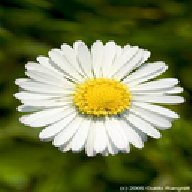
\includegraphics[width=0.22\textwidth]{./images/flower_19_image.pdf}
%     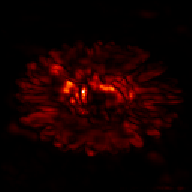
\includegraphics[width=0.22\textwidth]{./images/flower_19_topk_nat_orig.pdf}
%     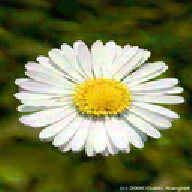
\includegraphics[width=0.22\textwidth]{./images/flower_19_image_pert.pdf}
%     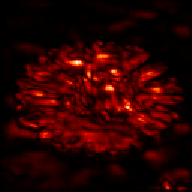
\includegraphics[width=0.22\textwidth]{./images/flower_19_topk_nat_pert.pdf}\\
%     \includegraphics[width=0.22\textwidth]{./images/flower_20_image.pdf}
%     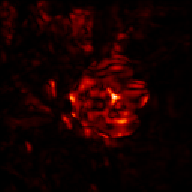
\includegraphics[width=0.22\textwidth]{./images/flower_20_topk_nat_orig.pdf}
%     \includegraphics[width=0.22\textwidth]{./images/flower_20_image_pert.pdf}
%     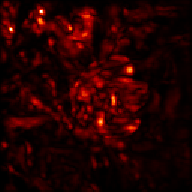
\includegraphics[width=0.22\textwidth]{./images/flower_20_topk_nat_pert.pdf}\\
%     \includegraphics[width=0.22\textwidth]{./images/flower_26_image.pdf}
%     \includegraphics[width=0.22\textwidth]{./images/flower_26_topk_nat_orig.pdf}
%     \includegraphics[width=0.22\textwidth]{./images/flower_26_image_pert.pdf}
%     \includegraphics[width=0.22\textwidth]{./images/flower_26_topk_nat_pert.pdf}\\
% \caption{Sample images from Flower dataset attributionally attack using \citet{ghorbani2018interpretation} method. Results obtained using a ResNet model.}
% \label{flower-samp-gh-nat}     
% \end{figure}
%
%For example for the image classification task, algorithms like Integrated Gradients\citep{x}, SmoothGrad, etc. based on the gradient of the loss function wrt the input obtain an explanation map which highlighs the parts of the image towards which importance is ``attributed'' by the model while classifying the image to a class. 
%This map which specifies which parts of the image the network focused on to take a decision, is expected to be in easy human interpretable form. These methods are largely known as ``post-hoc'' methods as an existing trained model's weights are used to find the explanation maps. \textcolor{blue}{Add more examples.} 
%
%While adversarial robustness has been very well-studied (Cite and summarize), the efforts on attributional robustness are far fewer (Cite and summarize). End with the motivation to embark on a work as what we have here.  \\
DNN-based models are known to have a vulnerability to imperceptible adversarial perturbations \citep{Biggio_2013,szegedy2014intriguing,goodfellow15fgsm}, which make them misclassify input images. %These small imperceptible perturbations are constructed using techniques like Fast Gradient Signed Method (FGSM) \citep{goodfellow15fgsm} and Projected Gradient Descent (PGD) \citep{madry2019deep}. %PGD \citep{madry2019deep} is currently the strongest adversarial attack. 
Adversarial training \citep{madry2019deep} is widely understood to provide a reasonable degree of robustness to such perturbation attacks. 
While adversarial robustness has received significant attention over the last few years \citep{ozdag2018advsurvey,silva2020advrobustsurvey}, the need for stable and robust attributions, corresponding explanation methods and their awareness are still in their early stages at this time \citep{ghorbani2018interpretation,chen2019robust,slack2020fooling,sarkar2020enhanced,lakkaraju2020icml,slack2021neurips-a,slack2021neurips-b}. In an early effort, \citep{ghorbani2018interpretation} provided a method to construct a small imperceptible perturbation which when added to an input $x$ results in a change in attribution map of the original map to that of the perturbed image. This is measured through top-$k$ intersection, Spearman's rank-order correlation or Kendall's rank-order correlation between the two attribution maps (of original and perturbed images). See Figure \ref{fig_intro} for an example. Defenses proposed against such attributional attacks %have also been proposed by regularizing the loss function or by using smoothing techniques on gradients 
\citep{chen2019robust,singh2020attributional,wang2020smoothed,sarkar2020enhanced}
%, which focus on regularizing the loss function \citep{chen2019robust,singh2020attributional,sarkar2020enhanced} or use smoothing techniques on gradients \citep{wang2020smoothed} to reduce the impact of the attack. 
also leverage the same metrics to evaluate the robustness of attribution methods.
%One of the earliest attacks on DNN model explanations or attributions was proposed in  \citep{ghorbani2018interpretation}, which is largely followed to the day. Example in Figure \ref{flower-samp-gh-nat}. 
%\begin{figure}[!ht]
%%\begin{wrapfigure}[21]{r}{0.5\textwidth}
%%\vspace{-10pt}
%  \begin{center}
%    % \includegraphics[width=0.12\textwidth]{./images/flower_12_image.pdf}
%    % \includegraphics[width=0.12\textwidth]{./images/flower_12_topk_nat_orig.pdf}
%    % \includegraphics[width=0.12\textwidth]{./images/flower_12_image_pert.pdf}
%    % \includegraphics[width=0.12\textwidth]{./images/flower_12_topk_nat_pert.pdf}\\
%    \includegraphics[width=0.11\textwidth]{./images/flower_20_image.pdf}
%    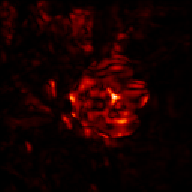
\includegraphics[width=0.11\textwidth]{./images/flower_20_topk_nat_orig.pdf}
%    \includegraphics[width=0.11\textwidth]{./images/flower_20_image_pert.pdf}
%    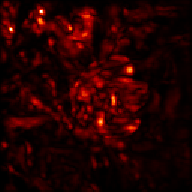
\includegraphics[width=0.11\textwidth]{./images/flower_20_topk_nat_pert.pdf}\\
%    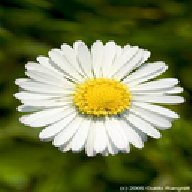
\includegraphics[width=0.11\textwidth]{./images/flower_19_image.pdf}
%    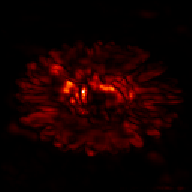
\includegraphics[width=0.11\textwidth]{./images/flower_19_topk_nat_orig.pdf}
%    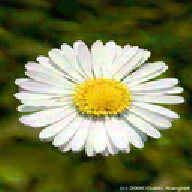
\includegraphics[width=0.11\textwidth]{./images/flower_19_image_pert.pdf}
%    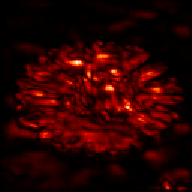
\includegraphics[width=0.11\textwidth]{./images/flower_19_topk_nat_pert.pdf}\\
%    % \includegraphics[width=0.12\textwidth]{./images/flower_26_image.pdf}
%    % \includegraphics[width=0.12\textwidth]{./images/flower_26_topk_nat_orig.pdf}
%    % \includegraphics[width=0.12\textwidth]{./images/flower_26_image_pert.pdf}
%    % \includegraphics[width=0.12\textwidth]{./images/flower_26_topk_nat_pert.pdf}\\
%  \end{center}
%  %\vspace{-10pt}
%  \caption{\footnotesize Attributional attack on Flower dataset using \citet{ghorbani2018interpretation} method on a ResNet model. Columns 1 and 3 show the image before and after an imperceptible perturbation; Columns 2 and 4 show the corresponding attributions. Note the change in attributions despite no perceptible change in input. \textbf{Row 1} shows a distinct change in top-$k$ pixels with the highest attribution; \textbf{Row 2} shows only a \textit{local change} in top-$k$ pixels with the highest attribution still within the object. The intersection between the top-$1000$ pixels before and after perturbation is less than $0.16$ in both the cases; thus, as a metric it cannot really distinguish the two. \textcolor{orange}{Image, top-1000, LENS, LENS-div}}
%  \label{fig_intro}
%%\end{wrapfigure}
%\end{figure}
%
\begin{figure}[!ht]
%\begin{wrapfigure}[21]{r}{0.5\textwidth}
%\vspace{-10pt}
  \begin{center}
    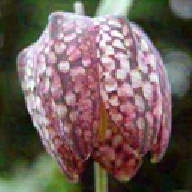
\includegraphics[width=0.15\textwidth]{./images/flower_10_image_pert.pdf}
    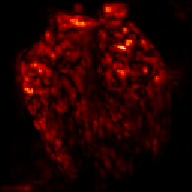
\includegraphics[width=0.15\textwidth]{./images/flower_10_topk_nat_orig.pdf}
    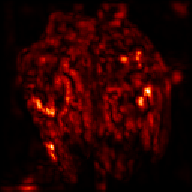
\includegraphics[width=0.15\textwidth]{./images/flower_10_topk_nat_pert.pdf}\\    
    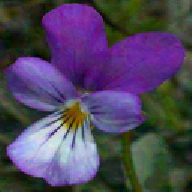
\includegraphics[width=0.15\textwidth]{./images/flower_4_image_pert.pdf}
    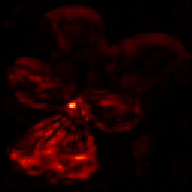
\includegraphics[width=0.15\textwidth]{./images/flower_4_topk_nat_orig.pdf}
    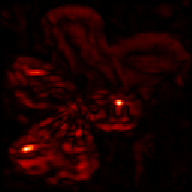
\includegraphics[width=0.15\textwidth]{./images/flower_4_topk_nat_pert.pdf}\\
    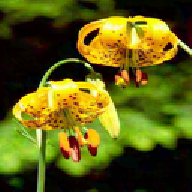
\includegraphics[width=0.15\textwidth]{./images/flower_18_image_pert.pdf}
    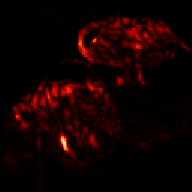
\includegraphics[width=0.15\textwidth]{./images/flower_18_topk_nat_orig.pdf}
    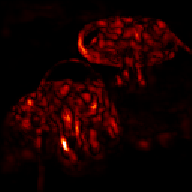
\includegraphics[width=0.15\textwidth]{./images/flower_18_topk_nat_pert.pdf}
  \end{center}
  \caption{Sample images from Flower dataset with Integrated Gradients (IG) before and after attributional attack. The attack used here is the top-$k$ attributional attack of \citet{ghorbani2018interpretation} on a ResNet model. Robustness of attribution measured by top-$k$ intersection is small, and ranges from 0.04 (first image) to 0.45 (third image) as it penalizes for both local changes in attribution and concentration of top pixels in a small region. Visually, we can observe that such overpenalization leads to a wrong sense of robustness as the changes are within the object of importance.}  
    %Column 3 shows a larger overlap in the union of $5 \times 5$-pixel neighborhoods around top-$k$ pixels, reflected in our locality-sensitive metrics 2-LENS-prec@$k$, 2-LENS-recall@$k$ valued 0.63 and 0.46, respectively. Column 4 shows an even larger overlap in the union of $5 \times 5$-pixel neighborhoods around the top-$k$ diverse pixels, reflected in our final metrics 2-LENS-pre@$k$-div and 2-LENS-recall@$k$-div valued 0.95 and 0.96, respectively. Note that only using top-$k$ diverse pixels and a metric that does not overpenalize local changes within $5 \times 5$-pixel neighborhood, the evaluation of robustness has changed from 0.13 to 0.96. Sample image from Flower dataset. (row 1) topk=0.31, 2-LEN 0.64,0.79, div 0.95,0.96, (row 2) topk=0.04, 2-LEN 0.25,0.23, div 0.96,0.96, (row 3) topk=0.45, 2-LEN 0.73,0.84, div 0.95,0.96.}
    %\caption{\footnotesize For $k=1000$, column 1 shows a sample image from Flower dataset before (top) and after (bottom) the top-$k$ attributional attack of \citet{ghorbani2018interpretation} on a ResNet model. Column 2 shows top-$k$ pixels for both images using Integrated Gradients (IG); the top-$k$ intersection is only 0.13 as it penalizes IG for both local changes in attribution and concentration of top pixels in a small region.  %Note the change in attributions despite no perceptible change in input. %\textbf{Row 1} shows a distinct change in top-$k$ pixels with the highest attribution; 
    %\textbf{Column 2} we observe only a \textit{local change} in top-$k$ pixels with the highest attribution still within the object. The intersection between the top-$1000$ pixels before and after perturbation is less than $0.14$; thus, as a metric top-$k$ intersection cannot really distinguish the two. 
    %Column 3 shows a larger overlap in the union of $5 \times 5$-pixel neighborhoods around top-$k$ pixels, reflected in our locality-sensitive metrics 2-LENS-prec@$k$, 2-LENS-recall@$k$ valued 0.63 and 0.46, respectively. Column 4 shows an even larger overlap in the union of $5 \times 5$-pixel neighborhoods around the top-$k$ diverse pixels, reflected in our final metrics 2-LENS-pre@$k$-div and 2-LENS-recall@$k$-div valued 0.95 and 0.96, respectively. Note that only using top-$k$ diverse pixels and a metric that does not overpenalize local changes within $5 \times 5$-pixel neighborhood, the evaluation of robustness has changed from 0.13 to 0.96. Sample image from Flower dataset. (row 1) topk=0.31, 2-LEN 0.64,0.79, div 0.95,0.96, (row 2) topk=0.04, 2-LEN 0.25,0.23, div 0.96,0.96, (row 3) topk=0.45, 2-LEN 0.73,0.84, div 0.95,0.96.}
  \label{fig_intro}
%\end{wrapfigure}
\end{figure}

%Across all the efforts so far \citep{ghorbani2018interpretation,chen2019robust,singh2020attributional,wang2020smoothed,sarkar2020enhanced}, the robustness of attributions on input perturbation is measured using metrics such as top-$k$ intersection, and rank correlations like Spearman's $\rho$ and Kendall' $\tau$ to estimate the quality of the attack. 
While these efforts have showcased the need and importance of studying the robustness of attribution methods, we note in this work that the metrics used, and hence the methods, can be highly sensitive to minor local changes in attributions (see Fig \ref{fig_intro} \textit{row 2}).
%such metrics give a reasonable estimate when there are significant changes in attributions, %(see Figure \ref{fig_intro} \textit{row 1})
We, in fact, show (in Appendix \ref{app:subsec:rand-vec}) that under existing metrics to evaluate robustness of attributions, a random perturbation can be as strong an attributional attack as existing benchmark methods. This may not be a true indicator of the robustness of a model's attributions, and can mislead further research efforts in the community. We hence focus our efforts in this work on rethinking metrics and methods to study the robustness of model attributions (in particular, we study image-based attribution methods to have a focused discussion and analysis). Beyond highlighting this important issue, we propose locality-sensitive improvements of the above metrics that incorporate the locality of attributions along with their rank order. We show that such a locality-sensitive distance is upper-bounded by a metric based on symmetric set difference. We also introduce a new measure {\bf top-$k$-div} that incorporates diversity of a model's attributions. % in the top-$k$ pixels picked. And show that infusing diversity and locality to observe the change between the explanation maps could be a better approach, thus providing an improved sense of attribution robustness. %One could also view existing methods that attempt to achieve attributional robusthe robust attribution methods proposed in recent works also reflect this premise of locality, thus highlighting the need for a locality-sensitive metric for progress in the field. %Our empirical results on well-known benchmark datasets using well-known models and attribution methods support our observations and conclusions in this work.
Our key contributions are summarized below:
%\vspace{-7pt}
%\noindent\textit{Our Results:}
\begin{itemize}[leftmargin=*]
\setlength\itemsep{-0.06em}
\item Firstly, we observe that existing robustness metrics for model attributions overpenalize minor drifts in attribution, leading to a false sense of fragility. %We go on to show that under existing such metrics, a random perturbation is as good an attack as principled methods like \citet{ghorbani2018interpretation}.
\item In order to address this issue, we propose Locality-sENSitive (LENS) improvements of existing metrics, namely, LENS-top-$k$, LENS-Spearman and LENS-Kendall, that incorporate the locality of attributions along with their rank order. Besides avoiding overpenalizing attribution methods for minor local drifts, we show that our proposed LENS variants are well-motivated by metrics defined on the space of attributions. %, and provide tighter bounds on the attributional robustness of already known improvements in attribution methods and model training designed for better attributions.
\item We subsequently introduce a second measure based on diversity that enriches model attributions by preventing the localized grouping of top model attributions. LENS can be naturally applied to this measure, thereby giving a method to incorporate both diversity and locality in measuring attributional robustness. 
\item Our comprehensive empirical results on benchmark datasets and models used in existing work clearly support our aforementioned observations, as well as the need to rethink the evaluation of the robustness of model attributions using locality and diversity. 
\item Finally, we also show that existing methods for robust attributions implicitly support such a locality-sensitive metric for evaluating progress in the field. 
%\item We show that the well established adversarial training with PGD for adversarial robustness could very well provide attributional robustness for free. \textcolor{blue}{Should we include this previously commented statement on PGD here. }
% \item Our metric for attributional robustness shows that random perturbation is not a strong attributional attack. We show the inherent fragility of attributions by showing it is vulnerable to even simple universal perturbation attack where a single random perturbation is added to all the samples is due to the local property not captured by previous metrics.
%\item \textcolor{red}{fragility of attributions, universal random perturbation attack}
%\item \textcolor{red}{adversarial robustness improves attributional robustness}
\end{itemize}
%
 %\vspace{-7pt}
\section{Background and Related Work}
\label{sec_related_work}
%\vspace{-7pt}
We herein discuss background literature from three different perspectives that may be related to our work: model explanation/attribution methods, efforts on attributional robustness (both attacks and defenses), and other recent related work.
%
\noindent \textbf{Attribution Methods.} Existing efforts on explainability in DNN models can be broadly categorized as: local and global methods, model-agnostic and model-specific methods, or as post-hoc and ante-hoc (intrinsically interpretable) methods \citep{molnar2019,xaitutorial}. Most existing methods in use today -- including methods to visualize weights and neurons \citep{simonyan2014deep,ZeilerF14}, guided backpropagation \citep{springenberg2015striving}, CAM \citep{ZhouKLOT16}, GradCAM \citep{Selvaraju_2019}, Grad-CAM++ \citep{Chattopadhay_2018}, LIME \citep{ribeiro2016why}, DeepLIFT \citep{shrikumar2017just,shrikumar2019learning}, LRP \citep{bach2015lrp}, Integrated Gradients \citep{SundararajanTY17}, SmoothGrad \citep{smilkov2017smoothgrad}), DeepSHAP \citep{lundberg2017unified} and TCAV \citep{kim2018interpretability} -- are post-hoc methods, which are used on top of a pre-trained DNN model to explain its predictions. We focus on such post-hoc attribution methods in this work. For a more detailed survey of explainability methods for DNN models, please see \citep{xaitutorial,molnar2019,samek_explainable_2019}. 
%
%\noindent \textbf{Strategies/Metrics for Evaluation of Attribution Methods on Images.}

\noindent \textbf{Robustness of Attributions.} The growing numbers of attribution methods proposed has also led to efforts on identifying the desirable characteristics of such methods \citep{alvarez2018robustness,AdebayoGMGHK18,yeh2019fidelity,ChalasaniC00J20,TomsettHCGP20,Boggust22Faithful,agarwal2022rethinking}. A key desired trait that has been highlighted by many of these efforts is robustness or stability of attributions, i.e., the explanation should not vary significantly within a small local neighborhood of the input \citep{alvarez2018robustness,ChalasaniC00J20}. \citet{ghorbani2018interpretation} showed that well-known methods such as gradient-based attributions, DeepLIFT \citep{shrikumar2019learning} and Integrated Gradients (IG) \citep{SundararajanTY17} are vulnerable to such input perturbations, and also provided an algorithm to construct a small imperceptible perturbation which when added to the input results in changes in the attribution.  \citet{slack2020fooling} later showed that methods like LIME \citep{ribeiro2016why} and DeepSHAP \citep{lundberg2017unified} are also vulnerable to such manipulations. The identification of such vulnerability and potential for attributional attacks has since led to multiple research efforts to make a model's attributions robust. \citet{chen2019robust} proposed a regularization-based approach, where an explicit regularizer term is added to the loss function to maintain the model gradient across input (IG, in particular) while training the DNN model. This was subsequently extended by \citep{sarkar2020enhanced,singh2020attributional,wang2020smoothed}, all of whom provide different training strategies and regularizers to improve attributional robustness of models. Each of these methods including \citet{ghorbani2018interpretation} measures change in attribution before and after input perturbation using the same metrics: top-$k$ intersection, and/or rank correlations like Spearman's $\rho$ and Kendall' $\tau$. Such metrics have recently, in fact, further been used to understand issues surrounding attributional robustness \citep{Wang22Kendall}. Other efforts that quantify stability of attributions in tabular data also use Euclidean distance (or its variants) between the original and perturbed attribution maps  \citep{alvarez2018robustness,yeh2019fidelity,agarwal2022rethinking}. Each of these metrics look for dimension-wise correlation or pixel-level matching between attribution maps before and after perturbation, and thus penalize even a minor change in attribution (say, even by one pixel coordinate location). This results in a false sense of fragility, and could even be misleading. In this work, we highlight the need to revisit such metrics, and propose variants based on locality and diversity that can be easily integrated into existing metrics. 

\noindent \textbf{Other Related Work.} In other related efforts that have studied similar properties of attribution-based explanations, \citep{carvalho2019machine,bhatt2020evaluating} stated that stable explanations should not vary too much between similar input samples, unless the model's prediction changes drastically. The abovementioned attributional attacks and defense methods \citep{ghorbani2018interpretation,sarkar2020enhanced,singh2020attributional,wang2020smoothed} maintain this property, since they focus on input perturbations that change the attribution without changing the model prediction itself. Similarly, \citet{arun2020assessing} and \citet{fel2022good} introduced the notions of repeatability/reproducibility and generalizability respectively, both of which focus on the desired property that a trustworthy explanation must point to similar evidence across similar input images. In this work, we provide a practical metric to study this notion of similarity by considering locality-sensitive metrics.
%
\section{{\bf L}ocality-s{\bf ENS}itive Metrics (LENS) for Attributional Robustness} \label{sec:lens}
%\vspace{-5pt}
 \begin{figure}[h]
 \centering
     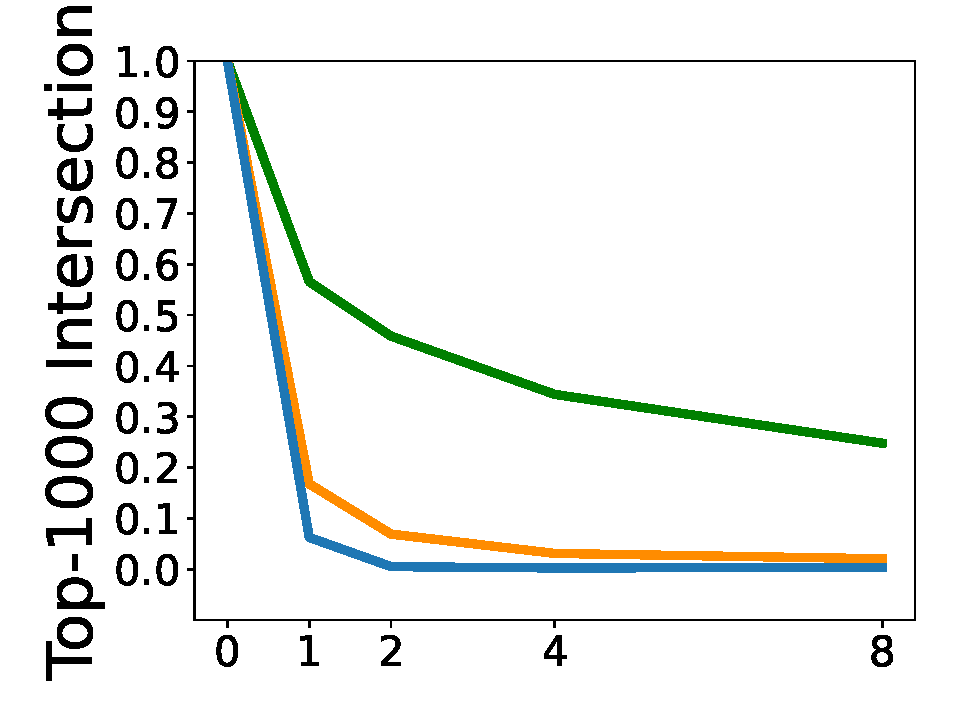
\includegraphics[width=0.22\textwidth]{./plots/imagenet_gh_lens_sg_orig_pert_all.pdf}
     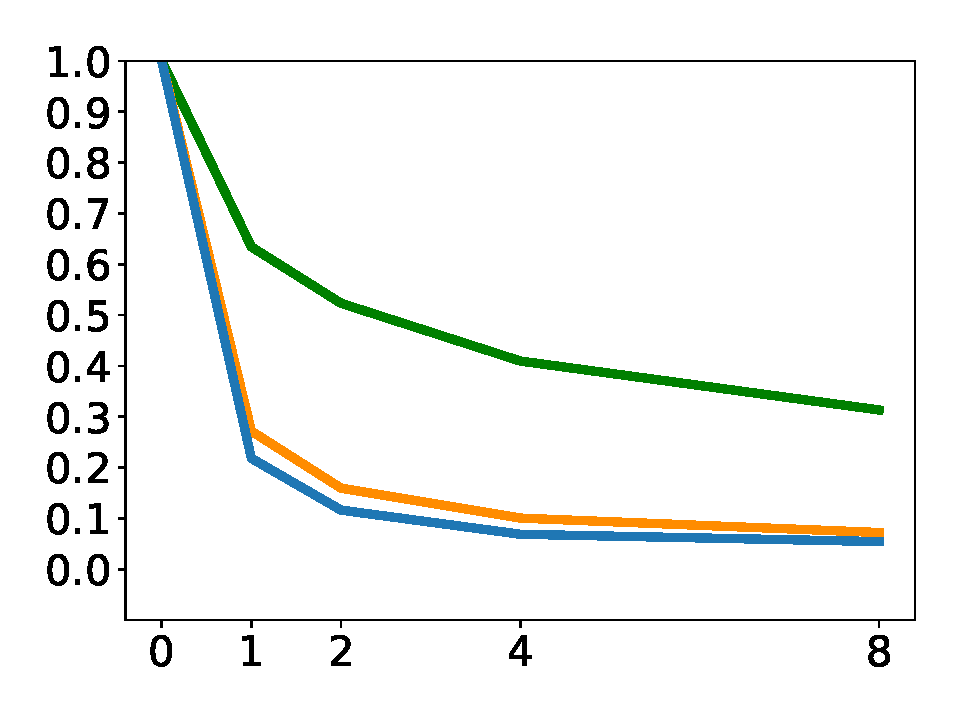
\includegraphics[width=0.22\textwidth]{./plots/imagenet_gh_lens_ig_orig_pert_all.pdf}\\
     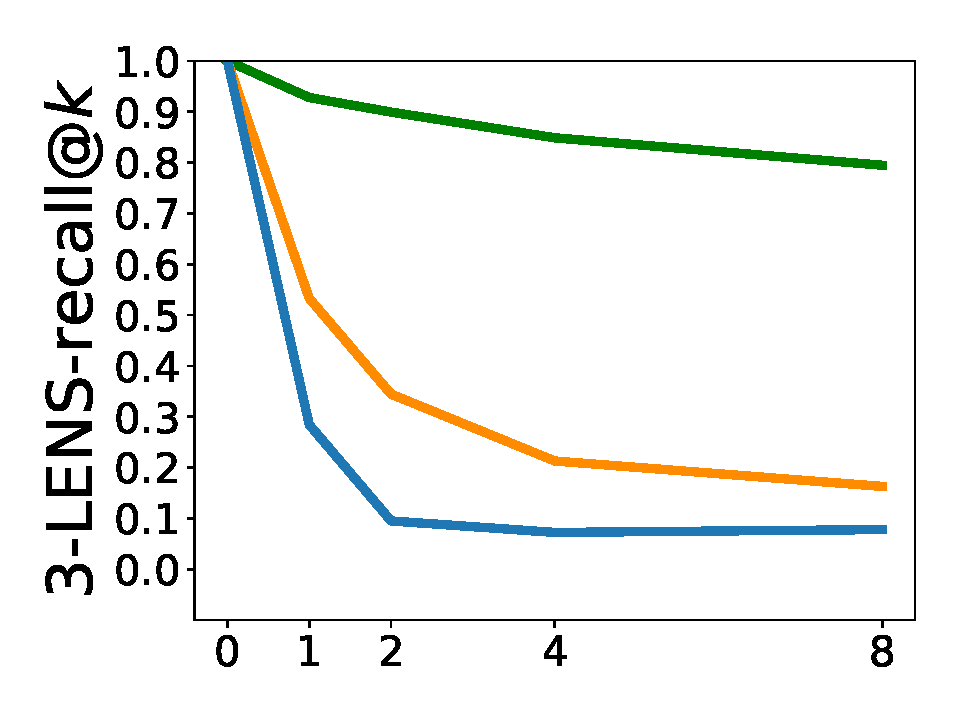
\includegraphics[width=0.22\textwidth]{./plots/imagenet_gh_lens_sg_orig_pert_all_lens.pdf}
     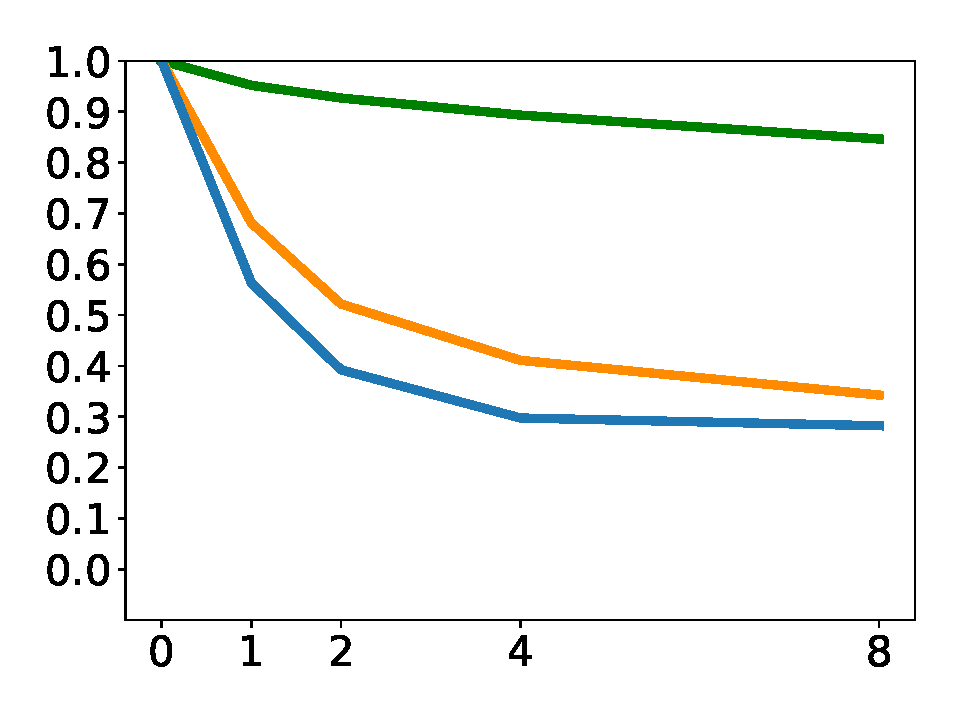
\includegraphics[width=0.22\textwidth]{./plots/imagenet_gh_lens_ig_orig_pert_all_lens.pdf}\\         
     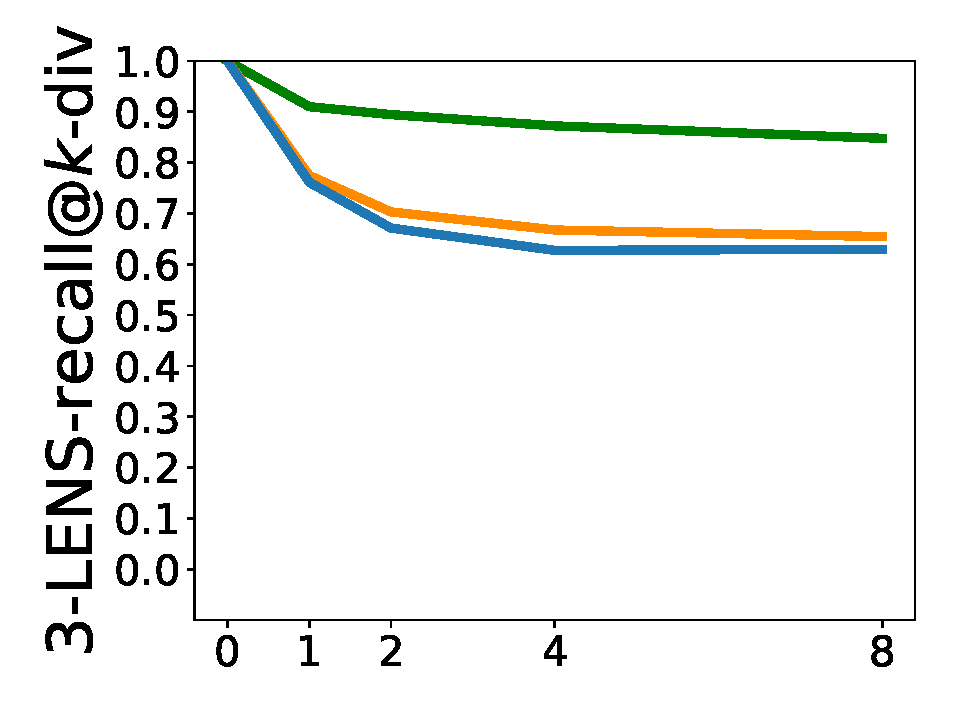
\includegraphics[width=0.22\textwidth]{./plots/imagenet_gh_lens_sg_orig_pert_all_div.pdf}
     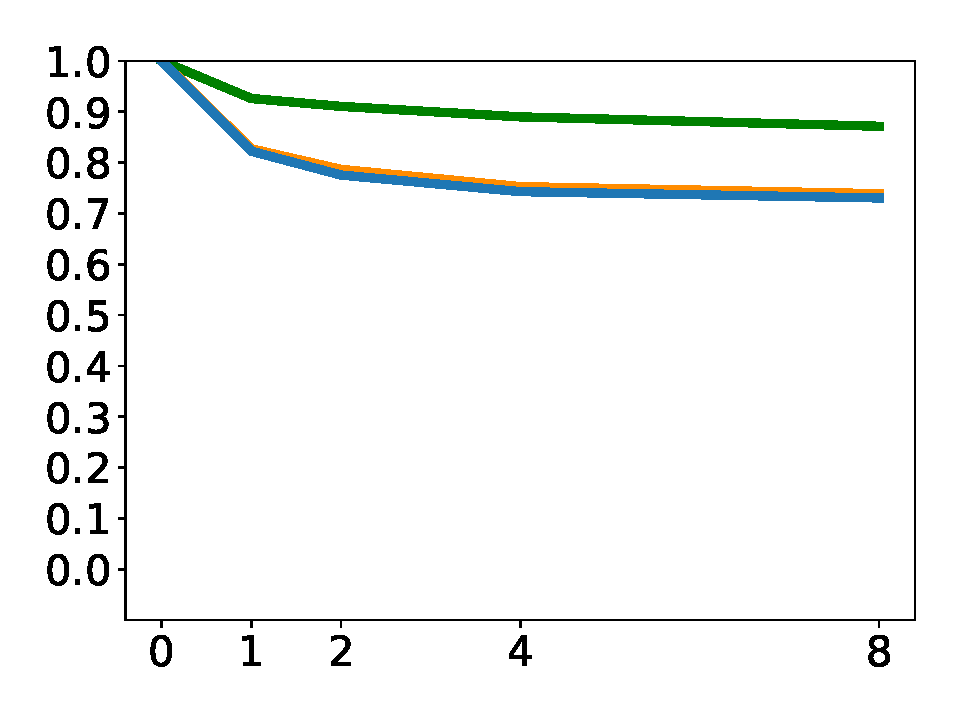
\includegraphics[width=0.22\textwidth]{./plots/imagenet_gh_lens_ig_orig_pert_all_div.pdf}    
    \caption{From top to bottom, we plot average top-$k$ intersection (currently used metric), $3$-LENS-recall@$k$ and $3$-LENS-recall@$k$-div (proposed metrics) against the $\ell_{\infty}$-norm of  attributional attack perturbations for Simple Gradients (SG) (left) and Integrated Gradients (IG) (right) of a SqueezeNet model on Imagenet. We use $k=1000$ and three attributional attack variants proposed by \citet{ghorbani2018interpretation}. Evidently, the proposed metrics show more robustness under the same attacks.}
\label{imagenet-ghorbani-with-lens-div}     
\end{figure}

As a motivating example, Figure \ref{imagenet-ghorbani-with-lens-div} presents the results obtained using \cite{ghorbani2018interpretation} with Simple Gradients (SG) and Integrated Gradients (IG) of an NN model trained on ImageNet. The top row, which reports the currently followed top-$k$ intersection measure of attribution robustness, shows a significant drop in robustness performance even for the random sign attack (green line). The subsequent rows, which report our metrics for the same experiments, show significant improvements in robustness -- especially when combining the notions of locality and diversity. Observations made on current metrics could lead to a false sense of fragility, which overpenalizes even an attribution shift by 1-2 pixels. A detailed description of our experimental setup for these results is available in Appendix \ref{app:exp-setup}. Motivated by these observations, we explore improved measures for attributional robustness that maintain the overall requirements of robustness, but do not overpenalize minor deviations.
%
%Note that the green line for random sign attack at $\epsilon=8/255$ in the top row indicates is close to top-$k$ and center of mass attacks indicating that under top-$k$ intersection measure of attribution robustness random could very well be a strong attack. These observations raises a strong need to look beyond current metrics used to study attributional robustness. Current analyses of attributional attacks use similarity measures such as top-$k$ intersection and rank correlation metrics such as Spearman's $\rho$, Kendall's $\tau$ that ignore where the top attributions are located in the image. As an aside, these are not \emph{metrics} in the mathematical sense but theoretically interesting metrics have been derived from them in the ranking literature \citep{fagin2003comparing}. This motivates us to explore to find a better measure of robustness which could incorporate more properties in the robustness measurement. This is precisely our we aim, to incorporate properties like locality and diversity into the robustness measure. We introduce LENS in this section for locality and top-$k$-div in Section \ref{sec:div-lens} incorporating diversity. Figure \ref{imagenet-ghorbani-with-lens-div} plots the improvement in attributional robustness with LENS and top-$k$-div. Figure \ref{fig_intro} provide sample visualization which aids us to reason why LENS and top-$k$-div are a strong impovement on the current top-$k$ intersection measure. 
%
%\textcolor{blue}{We conducted a survey to understand how well-aligned are the existing metrics with human perception. In Appendix \ref{app:survey-human}, we discuss the results of a survey which adds a new dimension to our study previously unexplored. We perform a survey to understand human perception of attribution maps along with the original image. We compare how much our new metric relates to human interpretation of attribution maps.}
%
\begin{figure}[!ht]
%\begin{wrapfigure}[21]{r}{0.5\textwidth}
%\vspace{-10pt}
  \begin{center}
    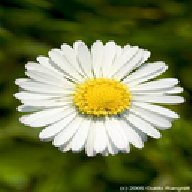
\includegraphics[width=0.11\textwidth]{./images/flower_19_image.pdf}
    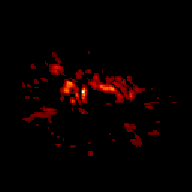
\includegraphics[width=0.11\textwidth]{./images/flower_19_topk_nat_orig_orig.pdf}
    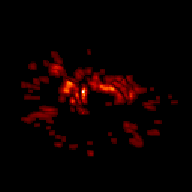
\includegraphics[width=0.11\textwidth]{./images/flower_19_topk_nat_orig_lens_rec.pdf}
    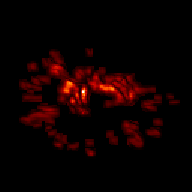
\includegraphics[width=0.11\textwidth]{./images/flower_19_topk_nat_orig_2lens_rec.pdf}\\
    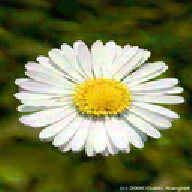
\includegraphics[width=0.11\textwidth]{./images/flower_19_image_pert.pdf}
    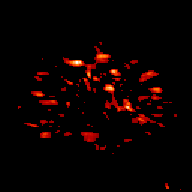
\includegraphics[width=0.11\textwidth]{./images/flower_19_topk_nat_orig_pert.pdf}
    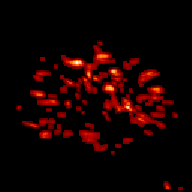
\includegraphics[width=0.11\textwidth]{./images/flower_19_topk_nat_orig_lens_pre.pdf}
    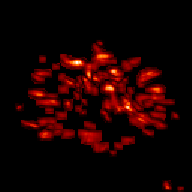
\includegraphics[width=0.11\textwidth]{./images/flower_19_topk_nat_orig_2lens_pre.pdf}\\
  \end{center}
  %\vspace{-10pt}
      \caption{A sample image from Flower dataset before (top) and after (bottom) the top-$k$ attributional attack of \cite{ghorbani2018interpretation} on a ResNet model for Integrated Gradients (IG) attribution method. From left to right: the image, its top-$k$ pixels as per IG, the union of the $3 \times 3$-pixel neighborhoods and $5 \times 5$-pixel neighborhoods of the top-$k$ pixels, respectively, for $k=1000$. Quantitatively, top-$k$ intersection: 0.14, 1-LENS-recall@$k$: 0.25, 1-LENS-pre@$k$: 0.37, 2-LENS-recall@$k$: 0.40, 2-LENS-pre@$k$: 0.62.} %\textit{Zoom images for finer details.}}
    \label{fig_intro_lens-19}
%\end{wrapfigure}
\end{figure}
%
%
%\vspace{-5pt}
\subsection{Defining LENS Metrics for Attributions} \label{subsec:define-lens}
%\subsection{Defining {\bf L}ocality-s{\bf ENS}itive Metrics for Attributions / Defining LENS for Attributions}
%\vspace{-5pt}
To begin with, we propose an extension of existing similarity measures to incorporate the locality of pixel attributions in images to derive more practical and useful measures of attributional robustness. Let $a_{ij}(x)$ denote the attribution value or importance assigned to the $(i, j)$-th pixel in an input image $x$, and let $S_{k}(x)$ denote the set of $k$ pixel positions with the largest attribution values. Let $N_{w}(i, j) = \{(p, q) \;:\; i-w \leq p \leq i+w,~ j-w \leq q \leq j+w\}$ be the neighboring pixel positions within a $(2w+1) \times (2w+1)$ window around the $(i, j)$-th pixel. By a slight abuse of notation, we use $N_{w}(S_{k}(x))$ to denote $\bigcup_{(i, j) \in S_{k}(x)} N_{w}(i, j)$, that is, the set of all pixel positions that lie in the union of $(2w+1) \times (2w+1)$ windows around the top-$k$ pixels. 

For a given attributional perturbation $\mathrm{Att}(\cdot)$, let $T_{k} = S_{k}(x + \mathrm{Att}(x))$ denote the top-$k$ pixels in attribution values after applying the attributional perturbation $\mathrm{Att}(x)$. The currently used top-$k$ intersection metric is then computed as: $\size{S_{k}(x) \cap T_{k}(x)}/k$. To address the abovementioned issues, we instead propose \emph{Locality-sENSitive top-$k$} metrics (LENS-top-$k$) as $\size{N_{w}(S_{k}(x)) \cap T_{k}(x)}/k$ and $\size{S_{k}(x) \cap N_{w}(T_{k}(x))}/k$, which are also closer to more widely used metrics such as precision and recall in ranking methods. We simiarly define Locality-sENSitive Spearman's $\rho$ (LENS-Spearman) and Locality-sENSitive Kendall's $\tau$ (LENS-Kendall) metrics as rank correlation coefficients for the smoothed ranking orders according to $\tilde{a}_{ij}(x)$'s and $\tilde{a}_{ij}(x + \mathrm{Att}(x))$'s, respectively. These can be used to compare two different attributions for the same image, the same attribution method on two different images, or even two different attributions on two different images, as long as the attribution vectors lie in the same space, e.g., images of the same dimensions where attributions assign importance values to pixels. Figure \ref{fig_intro_lens-19} provides the visualization of the explanation map of a sample from the Flower dataset with the top-1000 pixels followed by the corresponding maps with 1-LENS@$k$ and 2-LENS@$k$.

We show that the proposed locality-sensitive variants of the robustness metrics also possess some theoretically interesting properties. Let $\ba_{1}$ and $\ba_{2}$ be two attribution vectors for two images, and let $S_{k}$ and $T_{k}$ be the set of top $k$ pixels in these images according to $\ba_{1}$ and $\ba_{2}$, respectively. We define a locality-sensitive top-$k$ distance between two attribution vectors $\ba_{1}$ and $\ba_{2}$ as $d_{k}^{(w)}(\ba_{1}, \ba_{2})\overset{\text{def}}{=} \text{prec}_{k}^{(w)}(\ba_{1}, \ba_{2}) + \text{recall}_{k}^{(w)}(\ba_{1}, \ba_{2})$, where
$
%\vspace{-2pt}
\text{prec}_{k}^{(w)}(\ba_{1}, \ba_{2}) \overset{\text{def}}{=} \frac{\size{S_{k} \setminus N_{w}(T_{k})}}{k} \quad \text{and} 
$
$
\quad \text{recall}_{k}^{(w)}(\ba_{1}, \ba_{2}) \overset{\text{def}}{=} \frac{\size{T_{k} \setminus N_{w}(S_{k})}}{k},
$
similar to precision and recall used in ranking literature, with the key difference being the inclusion of neighborhood items based on locality. Below we state a monotonicity property of $d_{k}^{(w)}(\ba_{1}, \ba_{2})$ and upper bound it in terms of the symmetric set difference of top-$k$ attributions. 
\begin{prop} \label{prop:monotone}
For any $w_{1} \leq w_{2}$, we have $d_{k}^{(w_{2})}(\ba_{1}, \ba_{2}) \leq d_{k}^{(w_{1})}(\ba_{1}, \ba_{2}) \leq \size{S_{k} \triangle T_{k}}/k$, where $\triangle$ denotes the symmetric set difference, i.e., $A \triangle B = (A \setminus B) \cup (B \setminus A)$.
\end{prop}
%\begin{proof}
%The inequalities follows immediately using $S \subseteq N_{w_{1}}(S) \subseteq N_{w_{2}}(S)$, for any $S$, and hence, $\size{S \setminus N_{w}(T)} \leq \size{S \setminus T}$, for any $S, T$ and $w$.
%\end{proof}
Combining $d_{k}^{(w)}(\ba_{1}, \ba_{2})$ across different values of $k$ and $w$, we can define a distance 
\[
%\vspace{-2pt}
d(\ba_{1}, \ba_{2}) = \sum_{k=1}^{\infty} \alpha_{k} \sum_{w=0}^{\infty} \beta_{w}~ d_{k}^{(w)}(\ba_{1}, \ba_{2}),
\] 
where $\alpha_{k}$ and $\beta_{w}$ be non-negative weights, monotonically decreasing in $k$ and $w$, respectively, such that $\sum_{k} \alpha_{k} < \infty$ and $\sum_{w} \beta_{w} < \infty$. We show that the distance defined above is upper-bounded by a metric similar to those proposed in \cite{fagin2003comparing} based on symmetric set difference of top-$k$ ranks to compare two rankings.
%\begin{prop}
%Let $\ba_{1}, \ba_{2}, \ba_{3} \in \R^{n \times n}$ be three attribution vectors, e.g., vectors of attribution values for pixels in three $n \times n$ images, respectively, and possibly obtained by three different attribution methods. Let $S_{k}, T_{k}, U_{k}$ be the set of top $k$ pixels in $\ba_{1}, \ba_{2}, \ba_{3}$, respectively. Then, assuming $1 \leq w \ll k$, the relative set differences over neighborhoods $N_{w}(S_{k}), N_{w}(T_{k})$ and $N_{w}(U_{k})$ satisfies a weak triangle inequality, namely,
%\[
%\frac{\size{N_{w}(S_{k}) \triangle N_{w}(U_{k})}}{\size{N_{w}(S_{k}) \cup N_{w}(U_{k})}} \leq 10w^{2} \left(\frac{\size{N_{w}(S_{k}) \triangle N_{w}(T_{k})}}{\size{N_{w}(S_{k}) \cup N_{w}(T_{k})}} + \frac{\size{N_{w}(T_{k}) \triangle N_{w}(U_{k})}}{\size{N_{w}(T_{k}) \cup N_{w}(U)}}\right).
%\]
%\end{prop}
%\begin{proof}
%\begin{align*}
%\frac{\size{N_{w}(S_{k}) \triangle N_{w}(U_{k})}}{\size{N_{w}(S_{k}) \cup N_{w}(U_{k})}} & \leq \frac{\size{N_{w}(S_{k}) \triangle N_{w}(U_{k})}}{(2w+1)^{2} k - (2w-1)(2w+1) k} \\
%& \qquad \qquad \qquad \text{because $\size{N_{w}(S_{k}) \cup N_{w}(U_{k})} \geq \size{N_{w}(S_{k})} = \bigcup_{(i, j) \in S_{k}} N_{w}(i, j)$} \\
%& \qquad \qquad \qquad \text{and $\bigcup_{(i, j) \in S_{k}} N_{w}(i, j) \geq (2w+\sqrt{k})^{2}$; the lower bound is} \\
%& \qquad \qquad \qquad \text{attained when all $k$ pixels in $S_{k}$ form a $\sqrt{k} \times \sqrt{k}$ grid} \\
%& \leq \frac{\size{N_{w}(S_{k}) \triangle N_{w}(T_{k})} + \size{N_{w}(T_{k}) \triangle N_{w}(U_{k})}}{(2w+\sqrt{k})^{2}} \\
%& \qquad \qquad \text{by the triangle inequality of symmetric set difference metric} \\
%& \leq \frac{(2w+1)^{2}}{\left(1 + \nicefrac{2w}{\sqrt{k}}\right)^{2}} \left(\frac{\size{N_{w}(S_{k}) \triangle N_{w}(T_{k})}}{(2w+1)^{2} k} + \frac{\size{N_{w}(T_{k}) \triangle N_{w}(U_{k})}}{(2w+1)^{2} k}\right) \\
%& \leq 10w^{2} \left(\frac{\size{N_{w}(S_{k}) \triangle N_{w}(T_{k})}}{\size{N_{w}(S_{k}) \cup N_{w}(T_{k})}} + \frac{\size{N_{w}(T_{k}) \triangle N_{w}(U_{k})}}{\size{N_{w}(T_{k}) \cup N_{w}(U_{k})}}\right) \quad \text{for $1 \leq w \ll k$}.
%\end{align*}
%\end{proof}
\begin{prop} \label{prop:metric}
$d(\ba_{1}, \ba_{2})$ defined above is upper-bounded by $u(\ba_{1}, \ba_{2})$ given by
\[
%\vspace{-2pt} 
u(\ba_{1}, \ba_{2}) = \sum_{k=1}^{\infty} \alpha_{k} \sum_{w=0}^{\infty} \beta_{w}~ \frac{\size{S_{k} \triangle T_{k}}}{k},
\]
and $u(\ba_{1}, \ba_{2})$ defines a bounded metric on the space of attribution vectors.
\end{prop}
%\begin{proof}
%Proof follows from Proposition \ref{prop:monotone} and using %the fact that symmetric set difference satisfies triangle %inequality.
%\end{proof}
Note that top-$k$ intersection, Spearman's $\rho$ and Kendall's $\tau$ do not take the attribution values $a_{ij}(x)$'s into account but only the rank order of pixels according to these values. We also define a locality-sensitive $w$-smoothed attribution as follows.
\[
%\vspace{-2pt}
\tilde{a}_{ij}^{(w)}(x) = \frac{1}{(2w+1)^{2}} \sum_{\substack{(p, q) \in N_{w}(i, j), \\ 1 \leq p, q \leq n}} a_{pq}(x)
\]
We show that the $w$-smoothed attribution leads to a contraction in the $\ell_{2}$ norm commonly used in theoretical analysis of simple gradients as attributions. 
\begin{prop} \label{prop:w-smoothed}
For any inputs $x, y$ and any $w \geq 0$, $\norm{\tilde{\ba}^{(w)}(x) - \tilde{\ba}^{(w)}(y)}_{2} \leq \norm{\ba(x) - \ba(y)}_{2}$.
\end{prop}
%\begin{proof}
%\begin{align*}
%\norm{\tilde{\ba}^{(w)}(x) - \tilde{\ba}^{(w)}(y)}_{2}^{2} & = \sum_{1 \leq i, j \leq n} \left(\tilde{a}_{ij}^{(w)}(x) - \tilde{a}_{ij}^{(w)}(y)\right)^{2} \\ 
%& = \sum_{1 \leq i, j \leq n} \frac{1}{(2w+1)^{4}} \left(\sum_{\substack{(p, q) \in N_{w}(i, j), \\ 1 \leq p, q \leq n}} \left(a_{pq}(x) - a_{pq}(y)\right)\right)^{2} \\
%& \leq \sum_{1 \leq i, j \leq n} \frac{(2w+1)^{2}}{(2w+1)^{4}} \sum_{\substack{(p, q) \in N_{w}(i, j), \\ 1 \leq p, q \leq n}} \left(a_{pq}(x) - a_{pq}(y)\right)^{2}~ \text{by Cauchy-Schwarz inequality} \\
%& = \frac{1}{(2w+1)^{2}} \sum_{1 \leq i, j \leq n} \sum_{\substack{(p, q) \in N_{w}(i, j), \\ 1 \leq p, q \leq n}} \left(a_{pq}(x) - a_{pq}(y)\right)^{2} \\
%& \leq \frac{(2w+1)^{2}}{(2w+1)^{2}} \sum_{1 \leq p, q \leq n} \left(a_{pq}(x) - a_{pq}(y)\right)^{2} \\
%& \qquad \text{because each $(p, q)$ appears in at most $(2w+1)^{2}$ possibles $N_{w}(i, j)$'s} \\
%& = \norm{\ba(x) - \ba(y)}_{2}^{2}.
%\end{align*}
%\end{proof}
%\vspace{-5pt}
Thus, any theoretical bounds on the attributional robustness of simple gradients in $\ell_{2}$ norm proved in previous works continue to hold for locality-sensitive $w$-smoothed gradients. For example, \cite{wang2020smoothed} show the following Hessian-based bound on simple gradients. For an input $x$ and a classifier or model defined by $f$, let $\nabla_{x}(f)$ and $\nabla_{y}(f)$ be the simple gradients w.r.t. the inputs at $x$ and $y$. Theorem 3 in \cite{wang2020smoothed} upper bounds the $\ell_{2}$ distance between the simple gradients of nearby points $\norm{x - y}_{2} \leq \delta$ as  $\norm{\nabla_{x}(f) - \nabla_{y}(f)}_{2} \lesssim \delta~ \lambda_{\text{max}}(H_{x}(f))$, where $H_{x}(f)$ is the Hessian of $f$ w.r.t. the input at $x$ and $\lambda_{\text{max}}(H_{x}(f))$ is its maximum eigenvalue. By Proposition \ref{prop:w-smoothed} above, the same continues to hold for $w$-smoothed gradients, i.e., $\norm{\tilde{\nabla}_{x}^{(w)}(f) - \tilde{\nabla}_{y}^{(w)}(f)}_{2} \lesssim \delta~ \lambda_{\text{max}}(H_{x}(f))$. The proofs of all the propositions above are included in Appendix \ref{app:proofs}.
%
%We propose a new metric where we include a window around the top-$k$ pixels of each map to capture the local robustness or flexibility of the pixel to move under the top-$k$ pixel definition. Let $S(x)$ be the original attribution map of the sample image x and $T(x)$ be the attribution map of the sample image attacked with \citep{ghorbani2018interpretation} attack. $S_{p}$ and $T_{p}$ be the $p$ top-$k$ pixels of the respective maps considered for comparison. Let $n \times n$ be the local window centered around each top-$k$ pixel under consideration. For example if $n=3$ then it is $3 \times 3$, which is a 3 by 3 window with one top-$k$ pixel considered at its center. We include all the pixels in the window along with the center top-$k$ pixel for comparison with the attacked attribution map or vice versa. If we consider the source map S then the set of pixels to be used for the analysis are all the pixels with each of the $p$ top-$k$ pixels along with the pixels in the $n \times n$ window around them.i.e. $\{S_{p} \cup \{\forall j \in \mathcal{B}_{S_{k}}, k=\{1,...,p\}\}\}$, using $n=3$ $\mathcal{B}_{S_{k}} = 3 \times 3$ window centered around $S_{k}$. top-$k$ metric is $|\{S_{p} \cup \{\forall j \in \mathcal{B}_{S_{k}}\}\} \cap T_{p}|/|T_{p}|$. Similarly, if the window is on the perturbed map side $|S_{p} \cap \{T_{p} \cup \{\forall j \in \mathcal{B}_{T_{k}}\}\}|/|S_{p}|$. So the corresponding \citep{ghorbani2018interpretation} attack with the new metric will be $-\underset{i \in \mathcal{B}}{\sum} S(x)_{i}$ where $\mathcal{B}=\{S_{p} \cup \{\forall j \in \mathcal{B}_{S_{k}}\}\}$. 
%So the metric on the S side is $|\{3 \times 3\}_{S_{p}} \cap T_{p}| / |T_{p}|$, it observes whether the set $T_{p}$ has better top-$k$ intersection with the expanded $S_{p}$ set. Similarly, if we consider the window around T the metric is $|S_{p}\cap \{3 \times 3\}_{T_{p}}| / |S_{p}|$. In this case it observes the set $S_{p}$ has better top-$k$ intersection with the expanded $T_{p}$ set. 

\subsection{Relevance to Attributional Robustness} \label{subsec:lens-relevance-robustness}
%\subsection{{\bf L}ocality-s{\bf ENS}itive (LENS) Attributional Robustness Metrics Are Stronger}
%\subsection{LENS a stronger Attributional Robustness Metrics.}
%\vspace{-5pt}
The top-$k$ intersection is a measure of similarity instead of distance. Therefore, in our experiments for attributional robustness, we use locality-sensitive similarity measures $w\text{-LENS-prec@}k$ and $w\text{-LENS-recall@}k$ to denote $1 - \text{prec}_{k}^{(w)}(\ba_{1}, \ba_{2})$ and $1 - \text{recall}_{k}^{(w)}(\ba_{1}, \ba_{2})$, respectively, where $\ba_{1}$ is the attribution of the original image and $\ba_{2}$ is the attribution of the perturbed image. For rank correlation coefficients such as Kendall's $\tau$ and Spearman's $\rho$, we compute $w$-LENS-Kendall and $w$-LENS-Spearman as the same Kendall's $\tau$ and Spearman's $\rho$ but computed on the locality-sensitive $w$-smoothed attribution map $\tilde{\ba}^{(w)}$ instead of the original attribution map $\ba$. We also study how these similarity measures and their resulting attributional robustness measures change as we vary $w$.
%\textcolor{red}{$k$ and remove this or point to Appendix \ref{app:more-lens-results}} $w$.
%
In this section, we measure the attributional robustness of Integrated Gradients (IG) on naturally trained models as top-$k$ intersection, $w$-LENS-prec@$k$ and $w$-LENS-recall@$k$ between the IG of the original images and the IG of their perturbations obtained by various attacks. The attacks we consider are the top-$t$ attack and the mass-center attack of \citet{ghorbani2018interpretation} as well as random perturbation. All perturbations have $\ell_{\infty}$ norm bounded by $\delta=0.3$ for MNIST, $\delta=0.1$ for Fashion MNIST, and $\delta=8/255$ for GTSRB and Flower datasets. 

The values of $t$ used to construct top-$t$ attacks of \citet{ghorbani2018interpretation} are $t=200$ on MNIST, $t=100$ on Fashion MNIST and GTSRB, $t=1000$ on Flower. In the robustness evaluations for a fixed $k$, we use $k=100$ on MNIST, Fashion MNIST, GTSRB, and $k=1000$ on Flower.

\paragraph{Comparison of top-$k$ intersection, $1$-LENS-prec@$k$ and $1$-LENS-recall@$k$.} 
Figure \ref{dataset-topk-new-metric-st-nat} shows that top-$k$ intersection penalizes IG even for small, local changes. $1$-LENS-prec@$k$ and $1$-LENS-recall@$k$ values are always higher in comparison across all datasets in our experiments. Moreover, on both MNIST and Fashion MNIST, $1$-LENS-prec@$k$ is roughly $2$x higher (above $90\%$) compared to top-$k$ intersection (near $40\%$). In other words, an attack may appear stronger under a weaker measure of attributional robustness, if it ignores locality. This increase clearly shows that the top-$k$ attack of \citet{ghorbani2018interpretation} appears to be weaker on these datasets as the proportional increase by using locality indicates that the attack is only creating a local change than previously thought. We can see that for MNIST, Fashion-MNIST and GTSRB for $<$ 20\% of the samples, the top-$k$ attack was able to make changes larger than what 1-LENS@$k$ could measure.
%\textcolor{red}{Meaningless results presented in Fig. \ref{dataset-topk-new-metric-st-nat}: While the values of the LENS metrics in this figure are higher, it is unclear what this means on its own. Further analysis or explanation would be helpful.}
%\textcolor{purple}{Obtaining similar plot in Figure \ref{dataset-topk-new-metric-st-nat} with ImageNet may not be useful as with 1-LENS the value will be small see Figure \ref{imagenet-topk-window-new-metric-nat-ig-lens}(left). Do we remove Fashion/GTSRB and include ImageNet. In ImageNet, topk with locality is WEAK only with diversity and LENS we get better results. HIGHLIGHT this.}

%\begin{wrapfigure}{r}{0.48\textwidth}
\begin{figure}[!ht]
%\vspace{-12pt}
\centering
    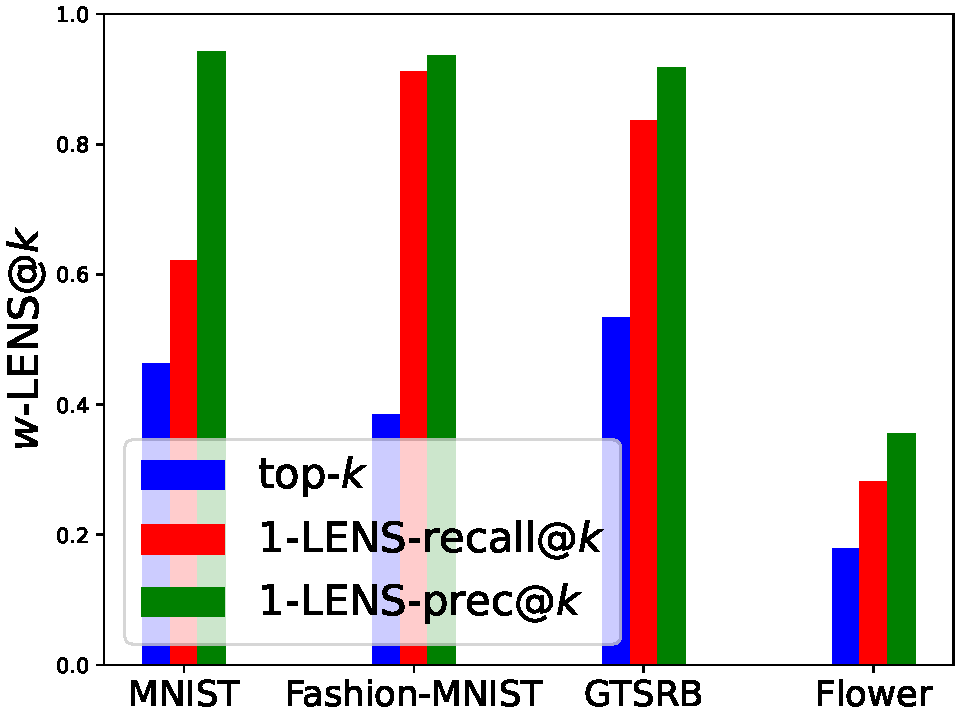
\includegraphics[width=0.25\textwidth]{./plots/datasets_topk_attack_nat_new_metric_1.pdf}
    %\vspace{-6pt}
\caption{Attributional robustness of IG on naturally trained models measured as average top-$k$ intersection, $1$-LENS-prec@$k$ and $1$-LENS-recall@$k$ between IG(original image) and IG(perturbed image) obtained by the top-$t$ attack \citep{ghorbani2018interpretation} across different datasets.} 
\label{dataset-topk-new-metric-st-nat}
%\vspace{-20pt}
%\end{wrapfigure}
\end{figure}

\begin{figure}[!ht]
%\begin{wrapfigure}{r}{0.48\textwidth}
\centering
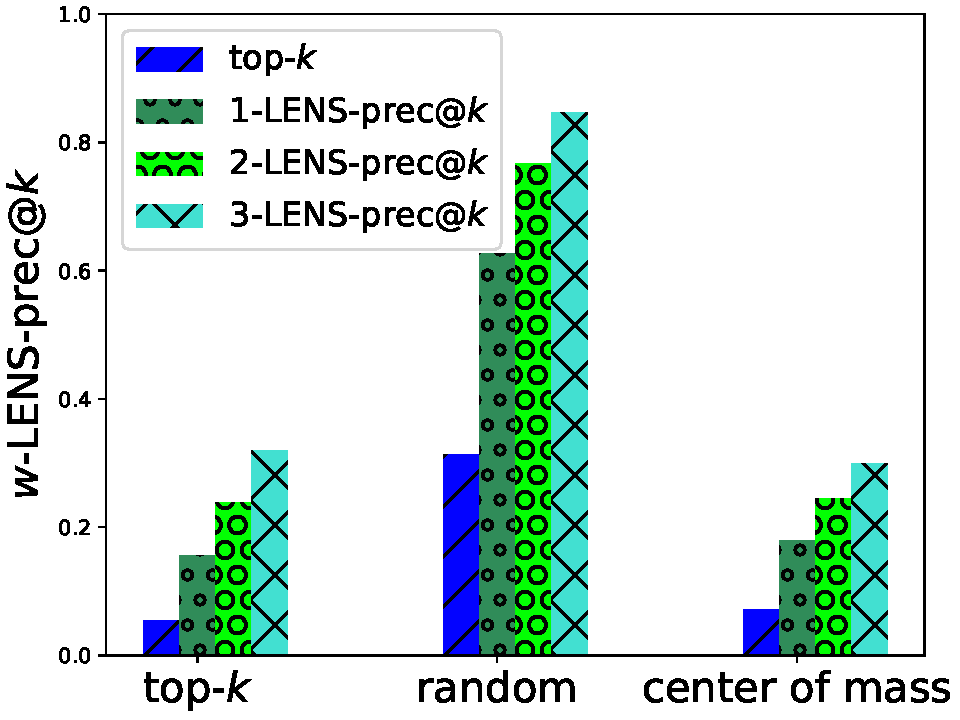
\includegraphics[width=0.22\textwidth]{./plots/imagenet_topk_attack_new_metric_nat_ig_lens.pdf}
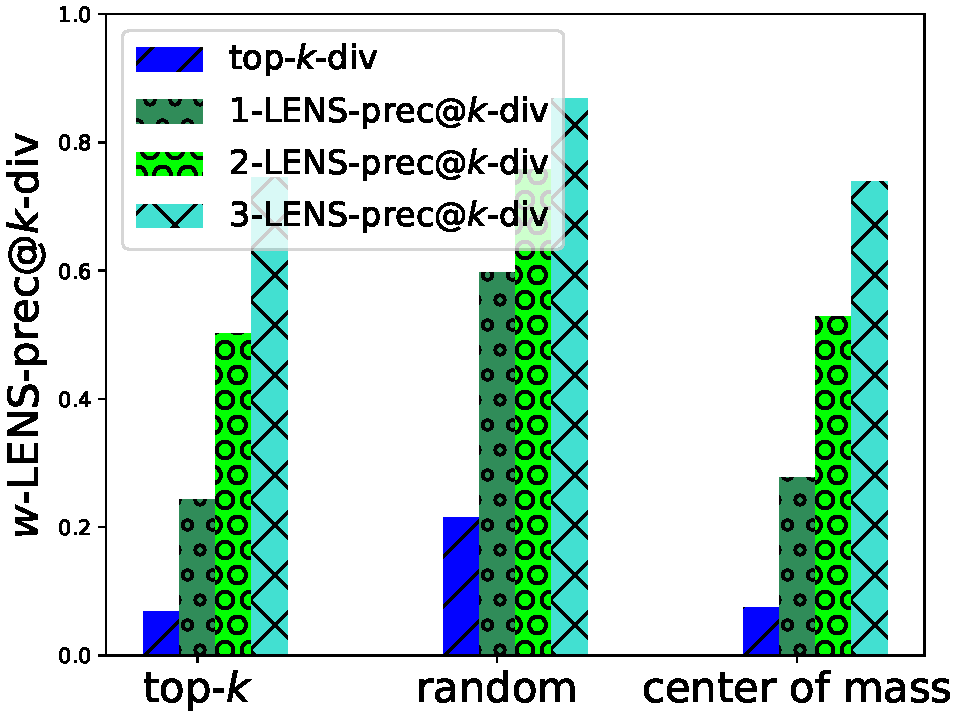
\includegraphics[width=0.219\textwidth]{./plots/imagenet_topk_attack_new_metric_nat_ig_lens_div.pdf}
\caption{Effect of increasing $w$ on average $w$-LENS-prec@$k$ and $w$-LENS-prec@$k$-div in comparison with top-$k$ intersection for IG map on ImageNet using a SqueezeNet model, when attacked with three attributional attacks (viz., top-$k$, random sign perturbation and mass center) of \citet{ghorbani2018interpretation}.}
\label{imagenet-topk-window-new-metric-nat-ig-lens} 
%\vspace{-5pt}
%\end{wrapfigure}
\end{figure}

%\vspace{-5pt}
\paragraph{$w$-LENS-prec@$k$ for varying $w$.} In Figure \ref{imagenet-topk-window-new-metric-nat-ig-lens}(left) $w$-LENS-prec@$k$ increases as we increase $w$ to consider larger neighborhoods around the pixels with top attribution values. This holds for multiple perturbations, namely, top-$t$ attack and mass-center attack by \citet{ghorbani2018interpretation} as well as a random perturbation. Notice that the top-$t$ attack of \citet{ghorbani2018interpretation} is constructed specifically for the top-$t$ intersection objective, and perhaps as a result, shows larger change when we increase local-sensitivity by increasing $w$ in the robustness measure. %\textcolor{orange}{Obtained similar Figure \ref{flower-topk-window-new-metric-nat-ig} with ImageNet with LENS (Figure \ref{imagenet-topk-window-new-metric-nat-ig-lens}) and Diversity (Figure \ref{imagenet-topk-window-new-metric-nat-ig-lens-div}).}
%\vspace{-12pt}
%\begin{figure}[!ht]
%%\vspace{-10pt}
%\centering
%\begin{minipage}{0.38\textwidth}
%\centering
%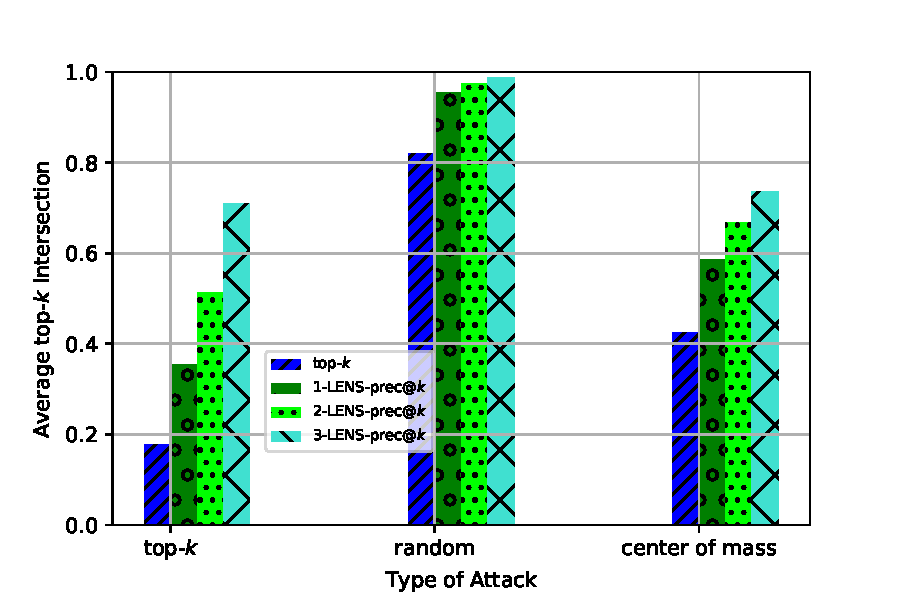
\includegraphics[width=\textwidth]{./plots/flower_topk_attack_new_metric_nat_ig.pdf}
%%\vspace{-6pt}
%\caption{\footnotesize Attributional robustness of IG on naturally trained models measured as average top-$k$ intersection and $w$-LENS-prec@$k$ between IG(original image) and IG(perturbed image). Perturbations are obtained by the top-$t$ attack and the mass-center attack \citep{ghorbani2018interpretation} as well as random perturbation. The plots show the effect of varying $w$ on Flower dataset.}
%\label{flower-topk-window-new-metric-nat-ig} 
%\end{minipage}\hfill
%\begin{minipage}{0.38\textwidth}
%\centering
%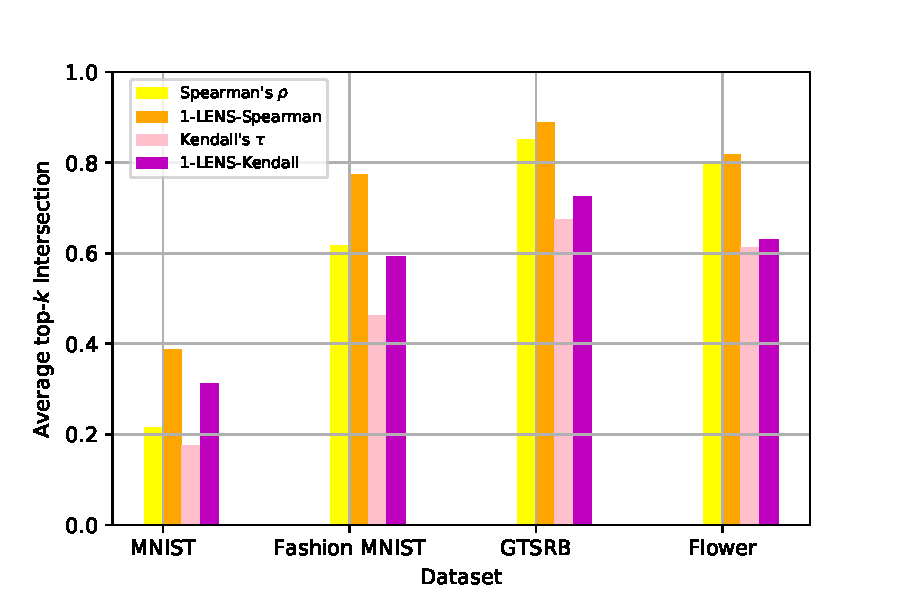
\includegraphics[width=\textwidth]{./plots/datasets_mean_filter_3x3_metrics_notopk.pdf}
%%\vspace{-6pt}
%\caption{\footnotesize Attributional robustness of IG on naturally trained models measured as average Spearman's $\rho$, $1$-LENS-Spearman, Kendall $\tau$ and $1$-LENS-Kendall between IG(original image) and IG(perturbed image). The perturbations are obtained by the top-$t$ attack of \citet{ghorbani2018interpretation}.} 
%\label{dataset-smooth-sp-ken-nat}
%\end{minipage}
%%\vspace{-20pt}
%\end{figure}

%\begin{figure}[!ht]
%\begin{wrapfigure}{r}{0.48\textwidth}
%\centering
%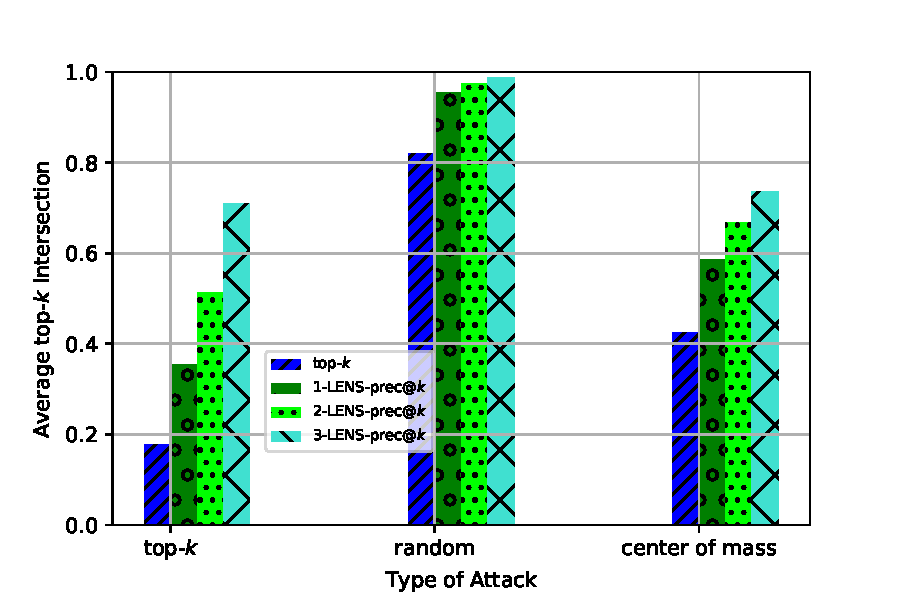
\includegraphics[width=0.38\textwidth]{./plots/flower_topk_attack_new_metric_nat_ig.pdf}
%\caption{\footnotesize Attributional robustness of IG on naturally trained models measured as average top-$k$ intersection and $w$-LENS-prec@$k$ between IG(original image) and IG(perturbed image). Perturbations are obtained by the top-$t$ attack and the mass-center attack \citep{ghorbani2018interpretation} as well as random perturbation. The plots show the effect of varying $w$ on Flower dataset.}
%\label{flower-topk-window-new-metric-nat-ig} 
%\vspace{-5pt}
%\end{wrapfigure}
%\end{figure}

Due to space constraint and purposes of coherence, we present few results with IG here; we present similar results on other explanation methods in the Appendix \ref{app:more-lens-results}. Refer to Appendix \ref{app:all-ig-exp} for similar plots with random sign perturbation and mass center attack of \citet{ghorbani2018interpretation}. Appendix \ref{app:all-sg-exp} contains additional results with similar conclusions when Simple Gradients are used instead of Integrated Gradients (IG) for obtaining the attributions. 

As a natural follow-up question we present in Appendix \ref{app:vary-k-sp-ken} results obtained by modifying the similarity objective of top-$k$ attack of \citet{ghorbani2018interpretation} with $1$-LENS-prec@$k$ with the assumption to obtain a stronger attack. But surprisingly, we notice that it leads to a \emph{worse} attributional attack, if we measure its effectiveness using the top-$k$ intersections and $1$-LENS-prec@$k$. In other words, attributional attacks against locality-sensitive measures of attributional robustness are non-trivial and may require fundamentally different ideas.

%\vspace{-10pt}
\subsection{Alignment of attributional robustness metrics to human perception}
\label{subsec:survey-human}
%\vspace{-7pt}

We conducted a survey with human participants, where we presented images from the Flower dataset and a pair of attribution maps---an attribution map of the original image alongside an attribution map of their random perturbation or attributional attacked version \citet{ghorbani2018interpretation}, in a random order and without revealing this information to the participants. The survey participants were asked whether the two maps were relatable to the image and if one of them was different than the other. In Table \ref{table-survey-results} we summarize the results obtained from the survey. We simplify the choices presented to the user into 2 final categories - \begin{inparaenum}[(1)] \item Agree with w-LENS-prec@$k$ \item Agree with top-$k$ metric \end{inparaenum} Category (1) includes all results where the user found the maps the same, relatable to the image but dissimilar or the perturbed map was preferred over the original map. Category (2) was the case where the user preferred the original map over the perturbed map. Refer to Appendix \ref{app:survey-human} for more details.

\begin{table}[!ht]
\vspace{-9pt}
\begin{center}
\resizebox{0.47\textwidth}{!}{ 
\begin{tabular}{|c|c|}
\hline 
{\bf Agree with 3-LENS-prec@$k$ metric(\%)} & {\bf Agree with top-$k$ metric(\%)} \\
\hline
70.37 & 29.63 \\ 
%81.48 & 18.52 \\ 
\hline
\end{tabular}
}
\vspace{-6pt}
\end{center}
\caption{Survey results based on humans ability to relate the explanation map to the original image with or without noise using the Flower dataset.}
\label{table-survey-results}
\end{table}

\begin{figure}[!ht]
%\begin{wrapfigure}[21]{r}{0.5\textwidth}
%\vspace{-10pt}
  \begin{center}
    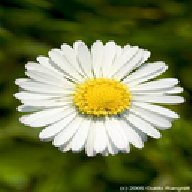
\includegraphics[width=0.11\textwidth]{./images/flower_19_image.pdf}
    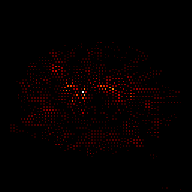
\includegraphics[width=0.11\textwidth]{./images/flower_19_topk_nat_orig_orig_div.pdf}
    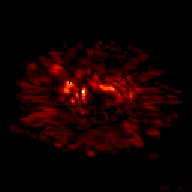
\includegraphics[width=0.11\textwidth]{./images/flower_19_topk_nat_orig_lens_rec_div.pdf}
    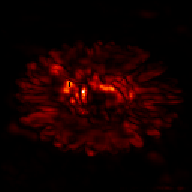
\includegraphics[width=0.11\textwidth]{./images/flower_19_topk_nat_orig_2lens_rec_div.pdf}\\
    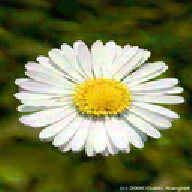
\includegraphics[width=0.11\textwidth]{./images/flower_19_image_pert.pdf}
    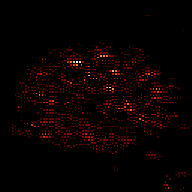
\includegraphics[width=0.11\textwidth]{./images/flower_19_topk_nat_orig_pert_div.pdf}
    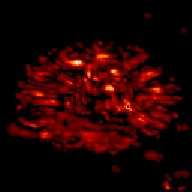
\includegraphics[width=0.11\textwidth]{./images/flower_19_topk_nat_orig_lens_pre_div.pdf}
    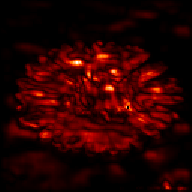
\includegraphics[width=0.11\textwidth]{./images/flower_19_topk_nat_orig_2lens_pre_div.pdf}\\
  \end{center}
  %\vspace{-10pt}
      \caption{A sample image from Flower dataset before (top) and after (bottom) the top-$k$ attributional attack of \citet{ghorbani2018interpretation} on a ResNet model. For both, we show from left to right: the image, its top-$k$ diverse pixels as per IG, the union of $3 \times 3$-pixel neighborhoods and $5 \times 5$-pixel neighborhoods of the top-$k$ diverse pixels, respectively, for $k=1000$. Quantitatively, improved overlap is captured by top-$k$-div intersection: 0.22, $1$-LENS-recall@$k$-div: 0.87, $1$-LENS-pre@$k$-div: 0.86, $2$-LENS-recall@$k$-div: 0.95, $2$-LENS-pre@$k$-div: 0.93. \emph{Zoom in required to see the diverse pixels.}}
  \label{fig_intro_div-19}
%\end{wrapfigure}
\end{figure}


\section{Diverse Attribution for Robustness} \label{sec:div-lens} 
Column 1 of Figure \ref{fig_intro_div-19} shows a typical  image from Flower dataset whose top-1000 pixels according to IG are concentrated in a small region. As seen in this illustrative example, when an image has multiple important parts, concentration of top attribution pixels in a small region increases vulnerability to attributional attacks. To alleviate this vulnerability, we propose post-processing any given attribution method to output top-$k$ \emph{diverse} pixels instead of just the top-$k$ pixels with the highest attribution scores. We use a natural notion of $w$-diversity based on pixel neighborhoods, so that these diverse pixels can be picked by a simple greedy algorithm. Starting with $S \leftarrow \emptyset$, repeat for $k$ steps: Pick the pixel of highest attribution score or importance outside $S$, add it to $S$ and disallow the $(2w+1) \times (2w+1)$-pixel neighborhood around it for future selection. The set of $k$ diverse pixels picked as above contains no two pixels within $(2w+1) \times (2w+1)$-pixel neighborhood of each other, and moreover, has the highest total importance (as the sum of pixel-wise attribution scores) among all such sets of $k$ pixels. The sets of $k$ pixels where no two pixels lie in $(2w+1) \times (2w+1)$-pixel neighborhood of each other form a matroid, where the optimality of greedy algorithm is well-known; see \citet{KorteLovasz1981}. 

Once we have the top-$k$ diverse pixels as described above, we can extend our locality-sensitive robustness metrics from the previous section to $w$-LENS-prec@$k$-div and $w$-LENS-recall@$k$-div, defined analogously using the union of $(2w+1) \times (2w+1)$-pixel neighborhoods of top-$k$ diverse pixels. In other words, define $\tilde{S}_{k}(x)$ as the top-$k$ diverse pixels for image $x$ and $\tilde{T}_{k} = \tilde{S}_{k}(x  + \text{Att}(x))$, and use $\tilde{S_{k}}$ and $\tilde{T}_{k}$ to replace $S_{k}$ and $T_{k}$ used in Subsection \ref{subsec:define-lens}. 

For $k=1000$, Figure \ref{fig_intro_div-19} shows a sample image from Flower dataset before and after the top-$k$ attributional attack of \citet{ghorbani2018interpretation}. Figure \ref{fig_intro_div-19} visually shows the top-$k$ diverse pixels in the Integrated Gradients (IG) and the union of their $(2w+1) \times (2w+1)$-pixel neighborhoods, for $w=\{1, 2\}$, for this image before and after the attributional attack. The reader may be required to zoom in to see the top-$k$ diverse pixels. See Appendix \ref{app:sample-fragility-examples} for more examples. Note that $0$-LENS-prec@$k$ and $0$-LENS-recall@$k$ are both the same and equivalent to top-$k$ intersection. However, a combined effect of locality and diversity can show a drastic leap from top-$k$ intersection value 0.14 to $2$-LENS-recall@$k$-div value 0.95 (see Fig.\ref{fig_intro_lens-19} and Fig.\ref{fig_intro_div-19}). Fig. \ref{imagenet-topk-window-new-metric-nat-ig-lens}(right) shows the effect of increasing $w$ on the $w$-LENS-prec@$k$-div metric on ImageNet.
%Figure \ref{fig_intro_div-19} (column 2) shows IG map from the Flower dataset highlighting only the top-1000 pixels. Column 3 and Column 4 in Figure \ref{fig_intro_div-19} present the corresponding top-$k$-div computed with 3x3 and 5x5 window, respectively. We suggest the reader to \textit{zoom} into Figure \ref{fig_intro_div-19}} to observe the spacing created by the nxn window among the chosen pixels to impose the diversity constraint. More detailed visualization available in Appendix \ref{app:sample-fragility-examples}. 

% COMMENTING OUT THE BELOW AS COMPARING DIFFERENT METRIC AGAINST DIFFERENTLY TRAINING FOR THE FINAL EFFECT IS NOT AN APPLES-TO-APPLES COMPARISON.
%\textcolor{purple}{We observe on a Natural trained network, diversity measurement improves drastically with LENS, does it indicate we don't need PGD and IG-SUM-NORM training under the diversity measurement for small datasets - MNIST, Fashion MNIST?} 

%\begin{table*}[!ht]
%\footnotesize
%\caption{Table with results with top-$k$ intersection and top-$k$ with diversity. First 3 columns correspond to top-$k$ intersection - top-$k$, 1-LENS-recall@$k$, 1-LENS-prec@$k$ followed by top-$k$ intersection with diversity - top-$k$-div, 1-LENS-recall@$k$-div, 1-LENS-prec@$k$-div. All results in the scale [0,1] for percentage multiply the value with 100.}
%\label{table-topk-div-results-imagenet}
%\begin{center}
%\resizebox{1.0\textwidth}{!}{ 
%\begin{tabular}{|l|l|c|c|c|c|c|c|c|c|}
%\hline 
%%Dataset & Training & Attack & {\bf Explanation method} & {\bf topk} & {\bf 1-LENS-recall@$k$ metric(\%)} &  {\bf 1-LENS-prec@$k$ metric(\%)} & {\bf topk-div} & {\bf 1-LENS-recall-div@$k$ metric(\%)} &  {\bf 1-LENS-prec-@$k$ metric(\%)} \\
%{\bf Dataset} & {\bf Train Type} & {\bf Attack Type} & {\bf Attribution Method} & {\bf top-$k$} & {\bf 1-LENS-recall@$k$} &  {\bf 1-LENS-prec@$k$} & {\bf top-$k$-div} & {\bf 1-LENS-recall@$k$-div} &  {\bf 1-LENS-prec@$k$-div} \\
%\hline
%ImageNet & Nat & top-$k$ & IG & 0.0544 & 0.1399 & 0.1555 & 0.0684 & 0.2384 & 0.2428 \\ 
%      & Nat & center of mass   & IG & 0.0722 & 0.1866 & 0.1789 & 0.0752 & 0.2802 & 0.2773\\ 
%      & Nat & random & IG & 0.3133 & 0.6216 & 0.6261 & 0.2157 & 0.5965 & 0.5969 \\ 
%\hline
%\end{tabular}
%}
%%\vspace{-6pt}
%\end{center}
%\end{table*}

\section{A Stronger Model for Attributional Robustness} \label{sec:adv-robust} 

%\begin{figure}[!ht]
%%\begin{wrapfigure}{r}{0.6\textwidth}
%%\vspace{-10pt}
%%\begin{figure}[!ht]
%\begin{minipage}{0.48\textwidth}
%\centering
%    \begin{subfigure}[b]{0.3\textwidth}
%    \includegraphics[width=\textwidth]{./images/flower_0_gh_2.pdf}
%    \caption{Sample Image}
%    \label{flower-sample-fig:a}
%    \end{subfigure}
%    \begin{subfigure}[b]{0.3\textwidth}
%    \includegraphics[width=\textwidth]{./images/flower_0_topk_pgd_orig.pdf}
%    \caption{IG of original}
%    \label{flower-sample-fig:b}
%    \end{subfigure}
%    \begin{subfigure}[b]{0.3\textwidth}
%    \includegraphics[width=\textwidth]{./images/flower_0_topk_pgd_pert.pdf}
%    \caption{IG of perturbed}
%    \label{flower-sample-fig:c}
%    \end{subfigure}\\
%    \begin{subfigure}[b]{0.3\textwidth}
%    \includegraphics[width=\textwidth]{./images/flower_0_gh_2.pdf}
%    \caption{Sample Image}
%    \label{flower-sample-fig:d}
%    \end{subfigure}
%    \begin{subfigure}[b]{.3\textwidth}
%    \includegraphics[width=\textwidth]{./images/flower_0_topk_rar_orig.pdf}
%    \caption{IG of original}
%    \label{flower-sample-fig:e}
%    \end{subfigure}
%    \begin{subfigure}[b]{0.3\textwidth}
%    \includegraphics[width=\textwidth]{./images/flower_0_topk_rar_pert.pdf}
%    \caption{IG of perturbed}
%    \label{flower-sample-fig:f}
%    \end{subfigure}
%    \caption{Sample image from Flower whose IG for PGD-trained (top) and IG-SUM-NORM trained (bottom) models seem robust to perturbations by the top-$k$ attack of \citet{ghorbani2018interpretation}.}
%\label{flower-sample-pgd-rar-topk}
%\end{minipage}
%%\vspace{-10pt}
%%\end{wrapfigure}
%\end{figure} 

%\begin{figure}[!ht]
%  \begin{center}
%    \includegraphics[width=0.15\textwidth]{./images/flower_0_gh_2.pdf}
%    \includegraphics[width=0.15\textwidth]{./images/flower_0_topk_pgd_orig.pdf}
%    \includegraphics[width=0.15\textwidth]{./images/flower_0_topk_pgd_pert.pdf}\\
%    \includegraphics[width=0.15\textwidth]{./images/flower_0_gh_2.pdf}
%    \includegraphics[width=0.15\textwidth]{./images/flower_0_topk_rar_orig.pdf}
%    \includegraphics[width=0.15\textwidth]{./images/flower_0_topk_rar_pert.pdf}
%  \end{center}
%      \caption{(left column) Sample image from Flower dataset (center column) IG of unperturbed image (right column) IG of perturbed image with topk attack. (top row) PGD-trained (bottom row) IG-SUM-NORM trained models seem robust to perturbations by the top-$k$ attack of \citet{ghorbani2018interpretation}. \textit{Zoom images for finer details.}}
%\label{flower-sample-pgd-rar-topk}
%\end{figure} 

\begin{figure}[!ht]
  \begin{center}
    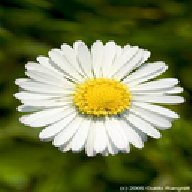
\includegraphics[width=0.15\textwidth]{./images/flower_19_image.pdf}
    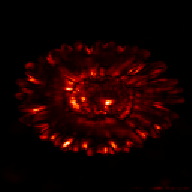
\includegraphics[width=0.15\textwidth]{./images/flower_19_topk_pgd_orig.pdf}
    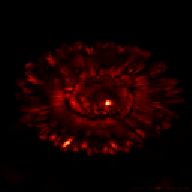
\includegraphics[width=0.15\textwidth]{./images/flower_19_topk_pgd_pert.pdf}\\
    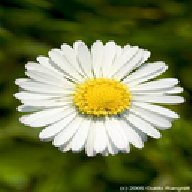
\includegraphics[width=0.15\textwidth]{./images/flower_19_image.pdf}
    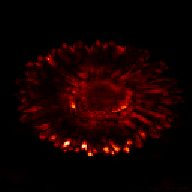
\includegraphics[width=0.15\textwidth]{./images/flower_19_topk_rar_orig.pdf}
    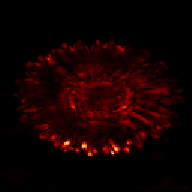
\includegraphics[width=0.15\textwidth]{./images/flower_19_topk_rar_pert.pdf}
  \end{center}
      \caption{From left to right: a sample image from Flower dataset and Integrated Gradients (IG) before and after the top-$k$ attributional attack of \citet{ghorbani2018interpretation}. The top row uses PGD-trained model whereas the bottom row uses IG-SUM-NORM-trained model.}
\label{flower-sample-pgd-rar-topk-19}
\end{figure} 


%
%\begin{figure}[!ht]
%\centering
%    \includegraphics[width=0.32\textwidth]{./images/flower_0_gh_2.pdf}
%    \includegraphics[width=0.32\textwidth]{./images/flower_0_topk_pgd_orig.pdf}
%    \includegraphics[width=0.32\textwidth]{./images/flower_0_topk_pgd_pert.pdf}
%\caption{Sample Ghorbani attacked image from Flower dataset. Adversarial(PGD) trained model.}
%\label{flower-samp-gh-pgd}     
%\end{figure}
%
%\begin{figure}[!ht]
%\centering
%    \includegraphics[width=0.32\textwidth]{./images/flower_0_gh_2.pdf}
%    \includegraphics[width=0.32\textwidth]{./images/flower_0_topk_rar_orig.pdf}
%    \includegraphics[width=0.32\textwidth]{./images/flower_0_topk_rar_pert.pdf}
%\caption{Sample Ghorbani attacked image from Flower dataset. RAR trained model.}
%\label{flower-samp-gh-rar}     
%\end{figure}
%
%\textcolor{red}{Adversarial robustness guards against the gradients $g(x)$, the direction of maximum change of the loss function at an input $x$, and therefore, it helps ensure that the prediction would not change. For attributional robustness, we need to guard against the top eigenvector of the Hessian $H(x)$. How do we do that?}
%
A common approach to get robust attributions is to keep the attribution method unchanged but train the models differently in a way that the resulting attributions are more robust to small perturbations of inputs. \citet{chen2019robust} proposed the first defense against the attributional attack of \citet{ghorbani2018interpretation}. \citet{wang2020smoothed} also find that IG-NORM based training of \citet{chen2019robust} gives models that exhibit attributional robustness against the top-$k$ attack of \citet{ghorbani2018interpretation} along with adversarially trained models. Figure \ref{flower-sample-pgd-rar-topk-19} shows a sample image from the Flower dataset, where the Integrated Gradients (IG) of the original image and its perturbation by the top-$k$ attack are visually similar for models that are either adversarially trained (trained using Projected Gradient Descent or PGD-trained, as proposed by \citep{madry2019deep}) or IG-SUM-NORM trained as in \citet{chen2019robust}. In other words, these differently trained model guard the sample image against the attributional top-$k$ attack. Recent work by \citet{nourelahi2022} has empirically studied the effectiveness of adversarially (PGD) trained models in obtaining better attributions, e.g., Figure \ref{flower-sample-pgd-rar-topk-19}(center) shows sharper attributions to features highlighting the ground-truth class.

\begin{figure}[!ht]
%\begin{wrapfigure}{r}{0.48\textwidth}
\centering
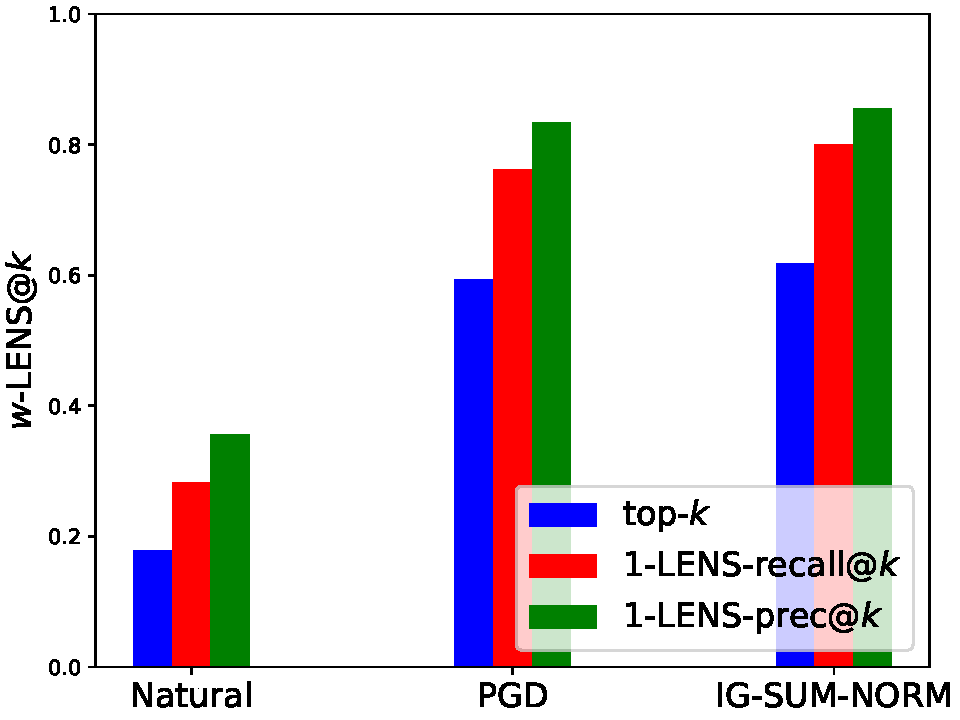
\includegraphics[width=0.219\textwidth]{./plots/flower_topk_3x3_attack_new_metric_1.pdf}
\caption{For Flower dataset, average top-$k$ intersection, $1$-LENS-prec@$k$, $1$-LENS-recall@$k$ measured between IG(original image) and IG(perturbed image) for models that are naturally trained, PGD-trained and IG-SUM-NORM trained. The perturbation used is the top-$t$ attack of \cite{ghorbani2018interpretation}. Note top-$k$ is equivalent to $0$-LENS-prec@$k$, $0$-LENS-recall@$k$.}
\label{flower-nat-pgd-rar-ig-diff-lens} 
%\vspace{-5pt}
%\end{wrapfigure}
\end{figure}

%We first formalize some notions about adversarial robustness. Let $\operatorname{Adv}_{\epsilon}(x)$ be an adversarial attack, e.g., FGSM, PGD etc. of $\ell_{\infty}$ norm $\epsilon$ (which particular adversarial attack we use should be evident from the context). Adversarial attack satisfies the following : $min ||\operatorname{Adv}(x)||_{\infty}, \text{subject to: } ||\operatorname{Adv}(x)||_{\infty} \leq \epsilon, f(x+\operatorname{Adv}(x);\mathcal{N}) \neq f(x;\mathcal{N})$. Adversarial training in the current strongest training method to defend against an adversarial attack. Adversarial training can be formulated as a min-max formulation $\underset{\theta}{min} \mathbb{E}_{(x,y) \in \mathcal{D}}\{\underset{\gamma \in \mathcal{B}}{max} \mathcal{L}(x+\gamma,y;\theta)\}$. $\mathcal{B}$ is of radius $\epsilon$, which is the perturbation budget. $\gamma$ is the perturbation obtain within the $\epsilon$-budget added to $x$ which leads to to the change of label $f(x) \neq f(x+\gamma)$. Currently, the strongest defense is adversarial training with PGD. Here, PGD is used to obtain the perturbed sample $x+\gamma$, which is used for training the network for in an epoch. The accuracy of the network under an adversarial attack is given by $\operatorname{Pr}(f(X+\operatorname{Adv}(x))=Y)$. Mainly, attributional attacks satisfy $f(x) = f(x+\operatorname{Att}_{\delta}(x))$ and adversarial attacks $f(x) \neq f(x+\operatorname{Adv}_{\epsilon}(x))$.

%Adversarial robustness(\citep{madry2019deep}) guards against perturbation in the direction of the maximum change in prediction loss, which is given by the gradient. Note that the first adversarial attack was FGSM that used the sign of the gradient. On the other hand the attributional robustness(\citep{chen2019robust}) requires guarding against the direction of the maximum change in the attribution itself. If we consider the gradient itself as a proxy for the gradient-based attribution, attributional robustness must guard against the direction of the maximum change in the gradient. This is a higher order problem. \citet{nourelahi2022} observe adversarial training aids better explanation maps and \citet{wang2020smoothed} show adversarial training aids attributional robustness too. By using the best of both worlds adversarially(PGD) trained model and attributionally trained model (\citet{chen2019robust}) with IG-SUM-NORM as the objective function to observe the effect of our LENS metric under various setting of the \citet{ghorbani2018interpretation} attack (top-$k$, random and mass-center). 
%We ask the following question -- Can adversarial robustness help solve a higher order problem? 

%Figure \ref{dataset-topk-new-metric-st-nat} we observed the impact of LENS on a naturally trained network. 
Figure \ref{flower-nat-pgd-rar-ig-diff-lens} shows that PGD-trained and IG-SUM-NORM trained models have more robust Integrated Gradients (IG) in comparison to their naturally trained counterparts, and this holds for the previously used measures of attributional robustness (e.g., top-$k$ intersection) as well as the new locality-sensitive measures we propose (e.g., $1$-LENS-prec@$k$, $1$-LENS-recall@$k$) across all datasets in \citet{chen2019robust} experiments (Refer Appendix \ref{app:all-ig-exp} and \ref{app:all-sg-exp}). The top-$k$ attack of \citet{ghorbani2018interpretation} is not a threat to IG if we simply measure its effectiveness using $1$-LENS-prec@$k$ (Appendix \ref{app:all-ig-exp}, \ref{app:all-sg-exp} for MNIST, Fashion MNIST and GTSRB). The above observation about robustness of Integrated Gradients (IG) for PGD-trained and IG-SUM-NORM trained models holds even when we use $1$-LENS-Spearman and $1$-LENS-Kendall measures to quantify the attributional robustness to the top-$k$ attack of \citet{ghorbani2018interpretation}, and it holds across the datasets used by \citet{chen2019robust} in their study; see Appendix \ref{app:more-lens-results}.

%\begin{figure}[!ht]
%\centering
%    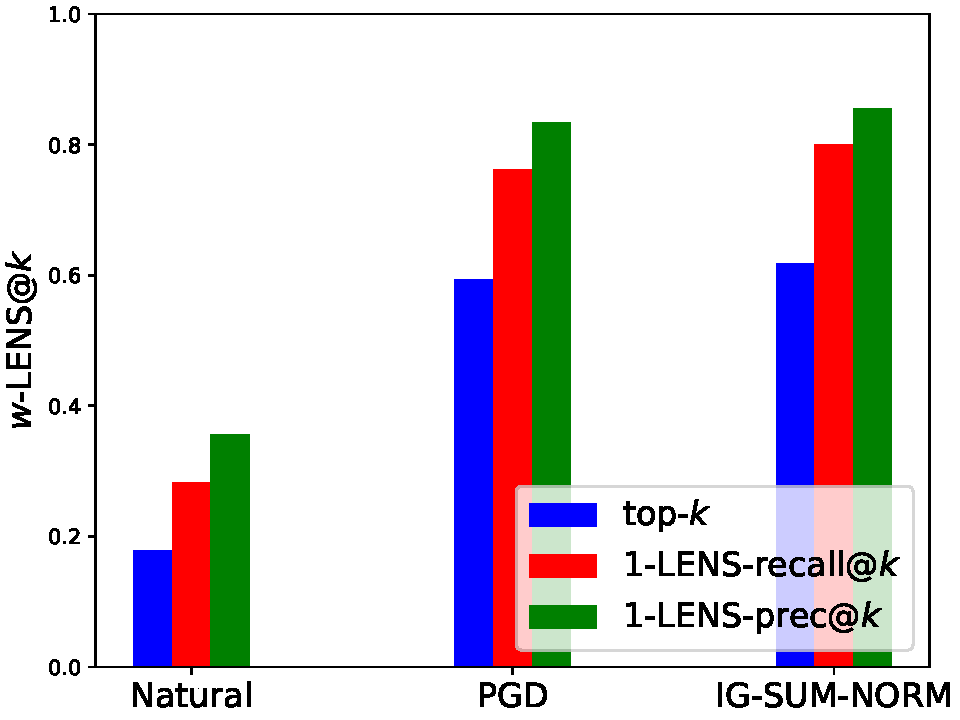
\includegraphics[width=0.4\textwidth]{./plots/flower_topk_3x3_attack_new_metric_1.pdf}
%\caption{For Flower dataset, average top-$k$ intersection, $1$-LENS-prec@$k$, $1$-LENS-recall@$k$ measured between IG(original image) and IG(perturbed image) for models that are naturally trained, PGD-trained and IG-SUM-NORM trained. The perturbation used is the top-$t$ attack of \cite{ghorbani2018interpretation}. Note top-$k$ is equivalent to $0$-LENS-prec@$k$, $0$-LENS-recall@$k$.}
%\label{flower-topk-new-metric-st-nat-pgd-rar}     
%\end{figure}

\citet{ChalasaniC00J20} show theoretically that $\ell_{\infty}$-adversarial training (PGD-training) leads to stable Integrated Gradients (IG) under $\ell_{1}$ norm. They also show empirically that PGD-training leads to sparse attributions (IG \& DeepSHAP) when sparseness in measured indirectly as the change in Gini index. Our empirical results extend their theoretical observation about stability of IG for PGD-trained models, as we measure local stability in terms of both the top attribution values and their positions in the image.

Table \ref{table-topk-div-results-rand-imagenet} obtains the top-$k$ intersection, 3-LENS-recall@$k$, and 3-LENS-recall@$k$-div of different attribution methods on ImageNet for naturally trained and PGD-trained ResNet50 models. We observe that for random sign attack the improvement obtained on top-$k$ intersection is reduced for a large dataset like ImageNet. Still our conclusions about locality and diversity in attribution robustness in comparison with the top-$k$ intersection baseline holds as we observe improvements in using diversity and locality. 
More results about incorporating diversity in the attribution and the resulting robustness metrics are available in Appendix \ref{app:extra-div-results}.
%
%\textcolor{blue}{More values are above 80\% indicating that top-$k$-div and $w$-LENS-prec@$k$ aptly capture locality and diversity as expected across explanation methods.} \textcolor{orange}{Observe BIG and GIG results here and in Table \ref{table-topk-div-results-rand} they show weaker results for PGD than Natural trained models.} Detailed results comparing diversity with $w$-LENS@$k$ available in Appendix \ref{app:extra-div-results}.

\begin{table}[!ht]    
%\vspace{-9pt}
\begin{center}
\resizebox{0.47\textwidth}{!}{ 
\begin{tabular}{|l|l|c|c|c|}
\hline 
%Dataset & Training & Attack & {\bf Explanation method} & {\bf topk} & {\bf 1-LENS-recall@$k$ metric(\%)} &  {\bf 1-LENS-prec@$k$ metric(\%)} & {\bf topk-div} & {\bf 1-LENS-recall-div@$k$ metric(\%)} &  {\bf 1-LENS-prec-div@$k$ metric(\%)} \\
{\bf Training} & {\bf Attribution method} & {\bf top-$k$} & {\bf 3-LENS-recall@$k$} & {\bf 3-LENS-recall@$k$-div} \\
\hline
Natural & Simple Gradient       & 0.3825 & 0.7875 & 0.8290 \\
Natural & Image $\times$ Gradient  & 0.3316 & 0.7765 & 0.8655 \\
Natural & LRP [Bach 2015]     & 0.1027 & 0.2487 & 0.7518 \\
Natural & DeepLIFT [Shrikumar 2017] & 0.2907 & 0.7641 & 0.8504 \\
Natural & GradSHAP [Lundberg 2017] & 0.2290 & 0.6513 & 0.8099 \\
Natural & IG [Sundararajan 2017]      & 0.2638 & 0.7148 & 0.8380 \\
%Natural & Blur IG [Xu 2020]    & 0.0520 & 0.3691 & 0.5266 \\
%Natural & Guided IG  [Kapishnikov 2021]    & 0.0850 & 0.6631 & 0.8078 \\
\hline 
PGD & Simple Gradient       & 0.1725 & 0.7245 & 0.8004 \\
PGD & Image $\times$ Gradient      & 0.1714 & 0.7269 & 0.8552 \\
PGD & LRP [Bach 2015] & 0.2374 & 0.4147 & 0.8161 \\
PGD & DeepLIFT [Shrikumar 2017] & 0.5572 & 0.9746 & 0.8977 \\
PGD & GradSHAP [Lundberg 2017] & 0.1714 & 0.7270 & 0.8552 \\
PGD & IG [Sundararajan 2017]      & 0.1947 & 0.7335 & 0.8584 \\
%PGD & Blur IG [Xu 2020]      & 0.0165 & 0.0524 & 0.4268 \\
%PGD & Guided IG  [Kapishnikov 2021]    & 0.0199 & 0.3378 & 0.6193 \\
\hline
\end{tabular}
}
\caption{Average top-$k$ intersection, 3-LENS-prec@$k$ and 3-LENS-prec@$k$-div for random sign perturbation attack applied to different attribution methods on ImageNet for naturally and adversarially(PGD)-trained ResNet50 models.}
\label{table-topk-div-results-rand-imagenet}
%\vspace{-6pt}
\end{center}
\end{table}
%
%
%\textcolor{blue}{Brief description of figures in this section.}
%Figure \ref{dataset-topk-new-metric-st-nat} we observed the impact of the new metric on a naturally trained network, Figure \ref{dataset-topk-new-metric-st-nat-pgd-rar} extends this study to adversarially(PGD) trained and attributional(IG-SUM-NORM) trained network. We can see that with our metric these methods provide strong defense to \citet{ghorbani2018interpretation} attack.
%
%Corresponding to Figure \ref{dataset-topk-rand-diff-k-new-metric-nat}, Figure \ref{dataset-topk-rand-diff-k-new-metric-pgd} and Figure \ref{dataset-topk-rand-diff-k-new-metric-rar}shows the impact of $k$ in top-$k$ for adversarially(PGD) trained and attributional(IG-SUM-NORM) trained network, respectively.
%
%Figure \ref{flower-topk-window-new-metric-nat-ig} showed the impact of new metric with changing window size on Flower dataset with natural trained network. Similarly, extends these observations with adversarially(PGD) trained and attributional(IG-SUM-NORM) trained network in Figure \ref{flower-topk-window-new-metric-nat-pgd-rar-ig}
%
%Figure \ref{dataset-smooth-sp-ken-nat-pgd-rar} observes the impact of LENS-Spearman and LENS-Kendall on adversarially(PGD) trained and attributional(RAR) trained network, similar to Figure \ref{dataset-smooth-sp-ken-nat}.
%
%\textcolor{blue}{End of brief description of figures in this section.}
%
%
%\paragraph{Results} \label{subsec:remedy:results}
%
%Let $\mathcal{M}_{\epsilon}$ be an adversarially trained model with adversarial attack $\operatorname{Adv}_{\epsilon}(x)$ of $\ell_{\infty}$ norm bounded by $\epsilon$. As $\epsilon$ increases, we check $\operatorname{E}[\mathcal{C}_{\operatorname{ken}}(\mathcal{I}(x), \mathcal{I}(X+\operatorname{Att}_{\delta}(X)))]$, where $\operatorname{Att}_{\delta}(x)$ is the attributional attack of \citep{ghorbani2018interpretation} of fixed norm $\delta$. As we increase $\epsilon$, the adversarial accuracy of $\mathcal{M}_{\epsilon}$ or its corresponding $\operatorname{Pr}(f(X+\operatorname{Adv}(X))=Y)$ increases. This is exactly as noticed by \citep{madry2019deep}. We want to check if the attributional robustness $\operatorname{E}[\mathcal{C}_{\operatorname{ken}}(\mathcal{I}(X), \mathcal{I}(x+\operatorname{Att}_{\delta}(X)))]$ also increases along with it. 
%We want to check this for different model architectures, different adversarial attacks $\operatorname{Adv}_{\epsilon}(x)$ and different attribution methods $\mathcal{I}(x)$.
%Figure \ref{sample-fmnist-pert-dir} to observe the maps and perturbations using Fashion-MNIST dataset with different trained networks. We show the impact of the new metric on different datasets under different training methods. Training methods are \begin{inparaenum} \item natural, \item adversarially trained(PGD) and \item RAR training as given by \citep{chen2019robust}\end{inparaenum}. Similar to Figure \ref{flower-topk-new-metric-training-method-nat} we have the plot on a PGD trained network in Figure \ref{flower-topk-new-metric-training-method-pgd}.
%
%In Figure \ref{delta-fixed-rand-adv-attr} we plot the accuracy and the correlation metrics for a naturally trained network and adversarially trained network with increasing $\epsilon$ budgets, attacked with input dependent random and topK attack of \citep{ghorbani2018interpretation} with a fixed $\delta$. As mentioned before currently, \citep{ghorbani2018interpretation} attack is the baseline attack for attributional robustness. This is to observe the change in attributional robustness with adversarial training in comparison with a naturally trained network. We observe in plots \ref{mnist-adv-fig:a} and \ref{flower-adv-fig:d} as expected $\operatorname{Pr}(f(X+Attr(X))=Y) \approx \operatorname{Pr}(f(X)=Y)$, but $\operatorname{Pr}(f(X)=Y)$ the natural accuracy drops with adversarial training as observed by \citep{Tsipras2019odds}. In plots \ref{mnist-adv-fig:b} and \ref{flower-adv-fig:e} we plot the correlation metrics using the topK attack of \citep{ghorbani2018interpretation} with a fixed $\delta$. We observe that with adversarial training the attributional robustness to this attack increases. In plots  \ref{mnist-adv-fig:c} and \ref{flower-adv-fig:f}, we show the impact of adversarial training towards input dependent random attack. We observe there is gains in comparison to naturally trained network. While in Figure \ref{delta-fixed-rand-adv-attr} we plot the observations for MNIST and Flower datasets. Refer to supplementary \ref{app:more-exp-remedy} for more results on Fashion MNIST and CIFAR10 datasets.
%
%
%In Section \ref{subsec:remedy:exp-setup}, we provide the details of experimental setup used in this study. Section \ref{subsec:remedy:results} we provide the details of the clear trend that with increasing $\epsilon$ budget for the adversarial training we obtain simultaneous attributional robustness to input dependent and \citet{ghorbani2018interpretation} attack. Section \ref{subsec:remedy:theory} provides the theoretical reasoning for the same. Figure \ref{mnist-sample-nat-adv-rand-topk} gives a sample from MNIST with IG maps with topk and random attack with $\delta=0.3$ for networks naturally trained in (Row 1) and adversarially trained with $\epsilon=0.3$ in (Row 2). It is visually clear that the IG maps have become better with adversarial training even under an attributional attack.
%
%We show the impact of the new metric on different datasets under different training methods. Training methods are 1. natural, 2. adversarially trained(PGD) and 3. RAR training as given by \citep{chen2019robust}. Similar to Figure \ref{flower-topk-new-metric-training-method-nat} we have the plot on a PGD trained network in Figure \ref{flower-topk-new-metric-training-method-pgd}.
%
%\textcolor{red}{\paragraph{Comparison with other methods}
%\citet{wang2020smoothed} have results with IG-NORM while IG-SUM-NORM obtains better results. They don't have any results using datasets which is comparable with original paper of \citet{chen2019robust}.}
%
%\paragraph{Observations for connection with other trained models}
%While \citep{chen2019robust} observe their regularization methods obtain better robustness to \citep{ghorbani2018interpretation} attack using the top-$k$ intersection, Spearman's $\rho$ and Kendall's $\tau$, we observe that using our LENS metric all the performance have boosted consistently above 80-90\% indicating that such models do show stronger locality robustness than a naturally trained model. Similar is also the case with adversarially trained models(\citet{nourelahi2022,wang2020smoothed). So our metric is able to show the equivalence between different methods capturing the local stability property well.}
%
%\vspace{-10pt}

\section{Conclusion and Future Work} \label{sec:conclusion}
We show that the fragility of attributions is an effect of using fragile robustness metrics such as top-$k$ intersection that only look at the rank order of attributions and fail to capture the locality of pixel positions with high attributions. We highlight the need for locality-sensitive metrics for attributional robustness and propose natural locality-sensitive extensions of existing metrics. We introduce another method of picking diverse top-$k$ pixels that can be naturally extended with locality to obtain improved measure of attributional robustness. Theoretical understanding of locality-sensitive metrics of attributional robustness, constructing stronger attributional attacks for these metrics, and using them to build attributionally robust models are important future directions. 

%\textcolor{red}{Currently we are around 8 pages. 7 pages is the limit.}
%\textcolor{blue}{Provide code in supplementary for reproducibility.}
%\textcolor{red}{\noindent \textbf{Reproducibility Statement.} The anonymous code for the paper can be found at this \href{https://anonymous.4open.science/r/anonymous-BEF2}{anonymous link}}.
%\clearpage
%\textcolor{red}{What are the other consequences of our results? What are the consequences of the fragility of attributional robustness? What are the consequences of adversarial robustness  implying attributional robustness? e.g., individual-fairness of interpretable decisions.}

\bibliography{anonymous-submission-latex-2024}
\bibliographystyle{aaai24}

\clearpage

\appendix
\section{Supplementary : Rethinking Robustness of Model Attributions}

The Appendix contains proofs, additional experiments to show that the trends hold across different datasets and other ablation studies which could not be included in the main paper due to space constraints. %\textcolor{purple}{Have not removed \\clearpage in appendix.If an algorithm depends on randomness, then the method used for setting seeds is described in a way sufficient to allow replication of results.}

%\section{Attributional Robustness Metrics are Weak, {\textcolor{blue}{Misaligned with Human Perception}}} \label{app:random-ext-fragile}
\section{Attributional Robustness Metrics are Weak} \label{app:random-ext-fragile}

%\vspace{-10pt}
%We first discuss the fragility of existing metrics, before presenting our locality-sensitive variants. The robustness of an attribution method has generally been measured in earlier work \citep{ghorbani2018interpretation,chen2019robust} by computing the similarity between attributions of an original input and the attribution of the same input with perturbations, and averaging this similarity across multiple input images.
%A generally accepted way to measure attributional robustness of an attribution method (e.g., Simple Gradients, Integrated Gradients, \textcolor{red}{Smooth Gradients}) in previous works \citep{ghorbani2018interpretation,chen2019robust} is by measuring the average similarity between the attributions for the original inputs and the attributions of their perturbations. 
%Similar to adversarial perturbations \citep{madry2019deep}, such ``attributional perturbations'' are carefully constructed attack vectors of small $\ell_{\infty}$ norm that do not change the model prediction but only the attributions on the perturbed inputs \citep{ghorbani2018interpretation}. Using this, \citet{ghorbani2018interpretation} show that many popular attribution methods are fragile. The common similarity measures between attributions are top-$k$ intersection and rank correlation coefficients such as Spearman's $\rho$ and Kendall's $\tau$. Note that all of the above similarity measures depend only on the rank order of features in the attributions (e.g., rank order of pixels in images).

In this section, we empirically show that the existing metrics for attributional robustness are weak and inadequate as they allow even a small random perturbation to appear like a decent attributional attack.

%\vspace{-10pt}
\subsection{Random Vectors are Attributional Attacks under Existing Metrics}
\label{app:subsec:rand-vec}
%\vspace{-7pt}
Random vectors of a small $\ell_{\infty}$ norm are often used as baselines of input perturbations (both in adversarial robustness \citep{silva2020advrobustsurvey} and attributional robustness literature \cite{ghorbani2018interpretation}), since it is known that predictions of neural network models are known to be resilient to random perturbations of inputs. 
Previous work by \citet{ghorbani2018interpretation} has shown random perturbations to be a reasonable baseline to compare against their attributional attack. Extending it further, we show that a single input-agnostic random perturbation happens to be an effective \emph{universal} attributional attack if we measure attributional robustness using a weak metric based on top-$k$ intersection. In other words, considering even a random perturbation happens to be a good attributional attack under such metrics, we show that existing metrics for attributional robustness such as top-$k$ intersection are extremely fragile, i.e., they would unfairly deem many attribution methods as fragile. 

Integrated Gradients (IG) is a well-known attribution method based on well-defined axiomatic foundations \citep{SundararajanTY17}, which is commonly used in attributional robustness literature \citep{chen2019robust,sarkar2020enhanced}. 
%{\textcolor{red}{Why IG? \citet{LundstromHR22} and \citet{NguyenKN21} respond to this paper.}}
We take a naturally trained CNN model on MNIST and perturb the images using a random perturbation (an independent random perturbation per input image) as well as a single, input-agnostic or \emph{universal} random perturbation for all images. Figure \ref{mnist-sample-nat-rand-topk} shows a sample image from the MNIST dataset and the visual difference between the IG of the original image, the IG after adding a random perturbation, and the IG after adding a \emph{universal} random perturbation. The IG after the universal random attack (Figure \ref{mnist-sample-fig:d}) is visually more dissimilar to the IG of the original image (Figure \ref{mnist-sample-fig:b}) than the IG of a simple random perturbation (Figure \ref{mnist-sample-fig:c}). (Note that top-$k$ intersection between Figure \ref{mnist-sample-fig:b} and \ref{mnist-sample-fig:c} is only 0.62, although the two look similar. As stated in the caption, a locality-sensitive metric shows them to be closer in attribution however.)
%\textcolor{red}{Missing quantitative comparisons and implementation details: There are important missing details. In particular, there is no quantitative comparison besides the cherry-picked result of Fig. 2 between the performance (in the standard metric sense) of the random perturbations and the current attacks. Moreover, it is in fact impossible to reproduce the results of this work as the way to obtain the smoothed versions of the standard metrics is not discussed.}

%\textcolor{red}{Lack of discussion on preservation of ordering/ranking with different metrics: There is no discussion on whether the ordering/ranking of different methods is preserved or not with standard metrics vs local ones. In my opinion, this is an important aspect missing of this work, because if the robustness ordering is still preserved with current standard metrics then there is less need for improvement using the LENS ones.}


%\vspace{-6pt}
\begin{figure}[!ht]
\centering
    \begin{subfigure}[b]{0.18\textwidth}
    
\includegraphics[width=\textwidth]{./images/mnist_sample_image_1.pdf}
    \caption{Original image}
    \label{mnist-sample-fig:a}
    \end{subfigure}
    \begin{subfigure}[b]{0.18\textwidth}
    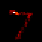
\includegraphics[width=\textwidth]{./images/mnist_sample_1_orig_ig.pdf}
    \caption{IG(original image)}
    \label{mnist-sample-fig:b}
    \end{subfigure}\\
    \begin{subfigure}[b]{0.18\textwidth}
    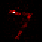
\includegraphics[width=\textwidth]{./images/mnist_sample_1_rand_03_ig.pdf}
    \caption{IG after random}
    \label{mnist-sample-fig:c}
    \end{subfigure}
    \begin{subfigure}[b]{0.18\textwidth}
    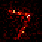
\includegraphics[width=\textwidth]{./images/mnist_sample_1_single_rand_03_ig.pdf}
    \caption{IG after universal}
    \label{mnist-sample-fig:d}
    \end{subfigure}
    %\vspace{-8pt}
    \caption{Sample image from MNIST on LeNet based model shows that the Integrated Gradients (IG) after a universal random perturbation are more dissimilar than IG after a simple, independent random perturbation for each input. All perturbations have random $\pm 1$ coordinates, scaled down to have $\ell_{\infty}$ norm $\epsilon=0.3$. (c) has a top-$k$ intersection of 0.68, while (d) has a top-$k$ intersection of 0.62. With our locality-sensitive metric, (c) has 1-LENS@$k$ of 0.99 and (d) has 1-LENS@$k$ of 1.0.}
    %\vspace{-6pt}
    %\caption{Sample examples from the MNIST dataset. (a,e) Original image, (b,f) Original IG, IG of sample perturbed by (c,g) input dependent random (d,h) single random perturbation with $\delta=0.3$.}
\label{mnist-sample-nat-rand-topk}
\end{figure} 

Similarly, Table \ref{table-rand-metric} shows that under existing metrics to quantify attributional robustness of IG on a naturally trained CNN model, even a single, input-agnostic or \emph{universal} random perturbation can sometimes be a more effective attributional attack than using an independent random perturbation for each input. %This observation particularly holds more strongly on MNIST and Fashion MNIST datasets. 
%The detailed description of our experimental setup can be found in Appendix \ref{app:exp-setup}.
\begin{table}[!ht]
\begin{center}
\resizebox{0.47\textwidth}{!}{ 
\begin{tabular}{|c|c|c|c|c|}
\hline 
%\multicolumn{1}{c}{\bf Dataset}  &\multicolumn{1}{c}{\bf Noise Type} &\multicolumn{1}{c}{\bf top-$k$ intersection} &\multicolumn{1}{c}{\bf Spearman's $\rho$} &\multicolumn{1}{c}{\bf Kendall's $\tau$}\\
{\bf Dataset} & {\bf Perturbation} & {\bf top-$k$ intersection} & {\bf Spearman's $\rho$} & {\bf Kendall's $\tau$} \\
\hline
MNIST & random & 0.7500 & 0.5347 & 0.4337 \\
& universal random & 0.5855 & 0.4831 & 0.4063 \\
\hline
Fashion MNIST & random & 0.5385 & 0.6791 & 0.5152 \\ 
& universal random & 0.5280 & 0.7154 & 0.5688 \\
\hline 
GTSRB & random & 0.8216 & 0.9433 & 0.8136 \\
& universal random & 0.9293 & 0.9887 & 0.9243 \\
\hline
Flower & random & 0.8202 & 0.9562 & 0.8340 \\ 
& universal random & 0.9344 & 0.9908 & 0.9321 \\ 
\hline
\end{tabular}
}
%\vspace{-6pt}
\end{center}
\caption{Attributional robustness of IG on naturally trained models measured using average top-$k$ intersection, Spearman's $\rho$ and Kendall's $\tau$ between IG(original image) and IG(perturbed image). $k=100$ for MNIST, Fashion MNIST, GTSRB and $k=1000$ for Flower. %{\bf Bold} entries indicate where the universal random perturbation is a stronger attributional attack.
}
%\vspace{-9pt}
\label{table-rand-metric}
\end{table}

%\clearpage

\section{Details of Experimental Setup} \label{app:exp-setup}
The detailed description of the setup used in our experiments.

\textit{Datasets:} We use the standard benchmark train-test split of all the datasets used in this work, that is publicly available. MNIST dataset consists of $70,000$ images of $28 \times 28$ size, divided into $10$ classes: $60,000$ used for training and $10,000$ for testing. Fashion MNIST dataset consists of $70,000$ images of $28 \times 28$ size, divided into $10$ classes: $60,000$ used for training and $10,000$ for testing. GTSRB dataset consists of $51,739$ images of $32 \times 32$ size, divided into $43$ classes: $34,699$ used for training, $4,410$ for validation and $12,630$ for testing. Flower dataset consist of $1,360$ images of $128 \times 128$ size, divided into $17$ classes: $1,224$ used for training and $136$ for testing. GTSRB and Flower datasets were preprocessed exactly as given in \cite{chen2019robust}[Appendix C] for consistency of results. ImageNet dataset consists of images of $227 \times 227$ size, divided into $1000$ classes. $50,000$ for validation were used to obtain samples for testing.

\textit{Architectures:} For MNIST, Fashion MNIST, GTSRB and Flower datasets we use the exact architectures as used by \citet{chen2019robust}, ImageNet dataset we use SqueezeNet\citep{IandolaMAHDK16} as given by \citet{ghorbani2018interpretation} and ResNet50\citep{HeZRS15}.

\textit{Attribution robustness metrics:} We use the same comparison metrics as used by \citet{ghorbani2018interpretation} and \citet{chen2019robust} like top-$k$ pixels intersection, Spearman's $\rho$ and Kendall's $\tau$ rank correlation to compare attribution maps of the original and perturbed images. The $k$ value for top-$k$ attack along with settings like step size, number of steps and number of times attack is to be applied is as used by \citet{chen2019robust} for the attack construction : MNIST(200,0.01,100,3), Fashion MNIST(100,0.01,100,3), GTSRB(100,1.0,50,3), Flower(1000,1.0,100,3) and ImageNet(1000,1.0,100,3) \citep{ghorbani2018interpretation}.

\textit{Sample sizes for attribution robustness evaluations:} \textit{IG based experiments} For MNIST, Fashion MNIST and Flower with fixed top-$k$ attack similar to \citet{chen2019robust} the complete test set were used to obtain the results. For GTSRB a random sample of size 1000 was used for all the experiments.  \textit{Simple gradient based experiments} For MNIST and Fashion MNIST a random sample of 2500/1000 from the test set. For GTSRB, a random sample of size 1000 and the complete test set for the Flower dataset. For ImageNet, we used the samples provide by \citet{ghorbani2018interpretation}. We used around 500 random samples for the random sign perturbation results using Pytorch/Captum.

\textit{Adversarial training:} We use the standard setup as used by \citep{chen2019robust}. We perform PGD based adversarial training with the provided $\epsilon$ budget using the following settings (number of steps, step size) for PGD : MNIST (40,0.01), Fashion MNIST(20,0.01), GTSRB(7,2/255), Flower(7,2/255). For ImageNet, we used the PGD based pre-trained ResNet50 model with $\ell_{\infty}$-norm of $\epsilon = 8/255$ provided in the robustness package\footnote{https://github.com/MadryLab/robustness/}.

\textit{Training for Attributional Robustness:} We use the IG-SUM-NORM objective function for all the datasets study based on \citep{chen2019robust} based training. With the exact setting as given in paper with code \footnote{https://github.com/jfc43/robust-attribution-regularization}.

\textit{Hardware Configuration:} We used a server with 4 Nvidia GeForce GTX 1080i GPU and a server with 8 Nvidia Tesla V100 GPU to run the experiments in the paper.

\textit{Explanation methods:} The Tensorflow \footnote{https://www.tensorflow.org} code for  IG, SG, DeepLIFT we used \citep{chen2019robust} and \citet{ghorbani2018interpretation} depending on the dataset. We used Pytorch\footnote{https://github.com/pytorch}- Captum\footnote{https://github.com/pytorch/captum} to obtain the various explanation maps with the random sign perturbation experiments.

\section{Proofs from Section \ref{subsec:define-lens}} \label{app:proofs}
We restate and prove Proposition \ref{prop:monotone} below.
\begin{prop} 
For any $w_{1} \leq w_{2}$, we have $d_{k}^{(w_{2})}(\ba_{1}, \ba_{2}) \leq d_{k}^{(w_{1})}(\ba_{1}, \ba_{2}) \leq \size{S_{k} \triangle T_{k}}/k$, where $\triangle$ denotes the symmetric set difference, i.e., $A \triangle B = (A \setminus B) \cup (B \setminus A)$.
\end{prop}
\begin{proof}
The inequalities follows immediately using $S \subseteq N_{w_{1}}(S) \subseteq N_{w_{2}}(S)$, for any $S$, and hence, $\size{S \setminus N_{w}(T)} \leq \size{S \setminus T}$, for any $S, T$ and $w$.
\end{proof}
We restate and prove Proposition \ref{prop:metric} below.
\begin{prop}
$d(\ba_{1}, \ba_{2})$ defined above is upper bounded by $u(\ba_{1}, \ba_{2})$ given by
\[
u(\ba_{1}, \ba_{2}) = \sum_{k=1}^{\infty} \alpha_{k} \sum_{w=0}^{\infty} \beta_{w}~ \frac{\size{S_{k} \triangle T_{k}}}{k},
\]
and $u(\ba_{1}, \ba_{2})$ defines a bounded metric on the space of attribution vectors.
\end{prop}
\begin{proof}
Proof follows from Proposition \ref{prop:monotone} and using the fact that symmetric set difference satisfies triangle inequality.
\end{proof}
We restate and prove Proposition \ref{prop:w-smoothed} below.
\begin{prop}
For any inputs $x, y$ and any $w \geq 0$, $\norm{\tilde{\ba}^{(w)}(x) - \tilde{\ba}^{(w)}(y)}_{2} \leq \norm{\ba(x) - \ba(y)}_{2}$.
\end{prop}
\begin{proof}

$\norm{\tilde{\ba}^{(w)}(x) - \tilde{\ba}^{(w)}(y)}_{2}^{2}$ 
\begin{align*}
&= \sum_{1 \leq i, j \leq n} \left(\tilde{a}_{ij}^{(w)}(x) - \tilde{a}_{ij}^{(w)}(y)\right)^{2} \\ 
& = \sum_{1 \leq i, j \leq n} \frac{1}{(2w+1)^{4}} \left(\sum_{\substack{(p, q) \in N_{w}(i, j), \\ 1 \leq p, q \leq n}} \left(a_{pq}(x) - a_{pq}(y)\right)\right)^{2} \\
& \leq \sum_{1 \leq i, j \leq n} \frac{(2w+1)^{2}}{(2w+1)^{4}} \sum_{\substack{(p, q) \in N_{w}(i, j), \\ 1 \leq p, q \leq n}} \left(a_{pq}(x) - a_{pq}(y)\right)^{2}~ 
\end{align*}
\text{by Cauchy-Schwarz inequality} \\

\begin{align*}
& = \frac{1}{(2w+1)^{2}} \sum_{1 \leq i, j \leq n} \sum_{\substack{(p, q) \in N_{w}(i, j), \\ 1 \leq p, q \leq n}} \left(a_{pq}(x) - a_{pq}(y)\right)^{2} \\
& \leq \frac{(2w+1)^{2}}{(2w+1)^{2}} \sum_{1 \leq p, q \leq n} \left(a_{pq}(x) - a_{pq}(y)\right)^{2} \\
& \qquad 
\end{align*}

because each $(p, q)$ appears in at most $(2w+1)^{2}$ possibles $N_{w}(i, j)$'s

\begin{align*}
& = \norm{\ba(x) - \ba(y)}_{2}^{2}.
\end{align*}
\end{proof}

%\clearpage 

\section{Additional results for Section \ref{sec:lens}} \label{app:more-lens-results}

\subsection{Additional results for Section \ref{subsec:lens-relevance-robustness}} \label{app:vary-k-sp-ken}
\paragraph{The effect of varying $k$.} Figure \ref{dataset-topk-rand-diff-k-new-metric-nat} shows a large disparity between top-$k$ intersection and $1$-LENS-prec@$k$ even when $k$ is large. Figure \ref{dataset-topk-rand-diff-k-new-metric-nat} shows that top-$k$ intersection can be very low even when the IG of the original and the IG of the perturbed images are locally very similar, as indicated by high $1$-LENS-prec@$k$. Our observation holds for the perturbations obtained by the top-$k$ attack \citep{ghorbani2018interpretation} as well as a random perturbation across all datasets in our experiments. Figure \ref{dataset-topk-rand-diff-k-new-metric-pgd} and \ref{dataset-topk-rand-diff-k-new-metric-rar} show the results on PGD and IG-SUM-NORM trained networks. 

\begin{figure}[!ht]
%\vspace{-20pt}
\centering
\begin{subfigure}[b]{1.0\textwidth}
    \begin{subfigure}[b]{0.12\textwidth}
    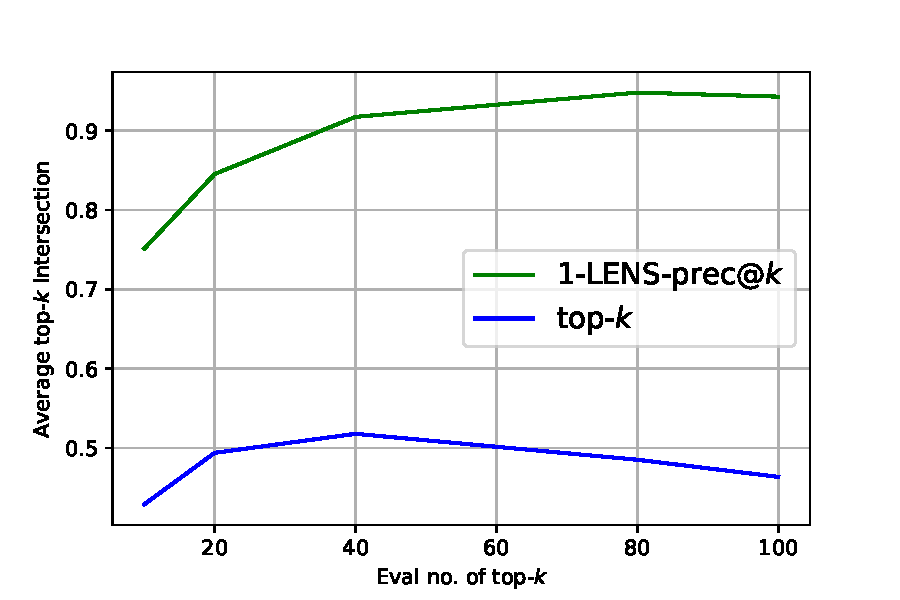
\includegraphics[width=1.0\textwidth]{./plots/mnist_topkvsrand_topk_nat.pdf}
    \caption{MNIST: top-$k$}
    \label{mnist-rand-fig:a}
    \end{subfigure}
    \begin{subfigure}[b]{0.12\textwidth}
    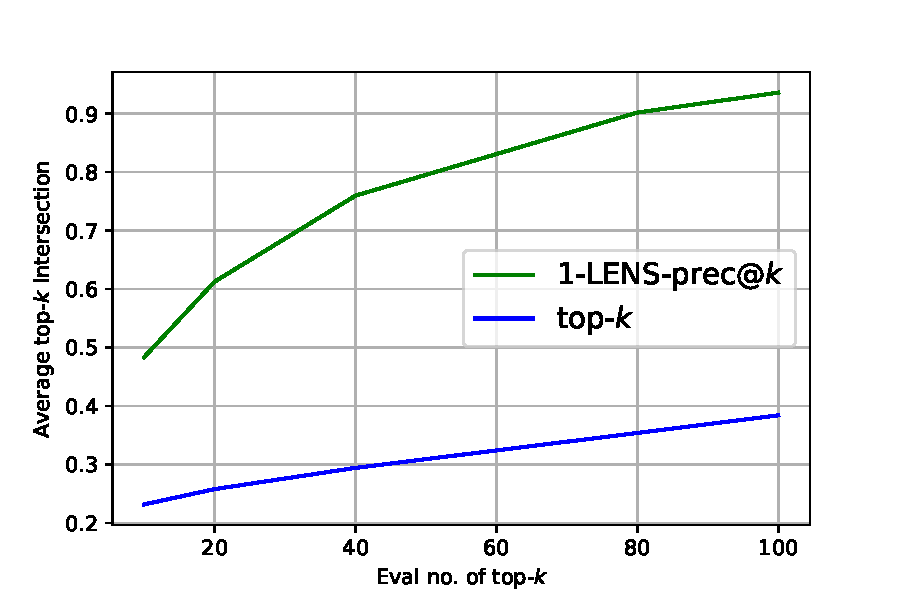
\includegraphics[width=1.0\textwidth]{./plots/fmnist_topkvsrand_topk_nat.pdf}
    \caption{F-MNIST: top-$t$}
    \label{mnist-rand-fig:b}
    \end{subfigure}
    \begin{subfigure}[b]{0.12\textwidth}
    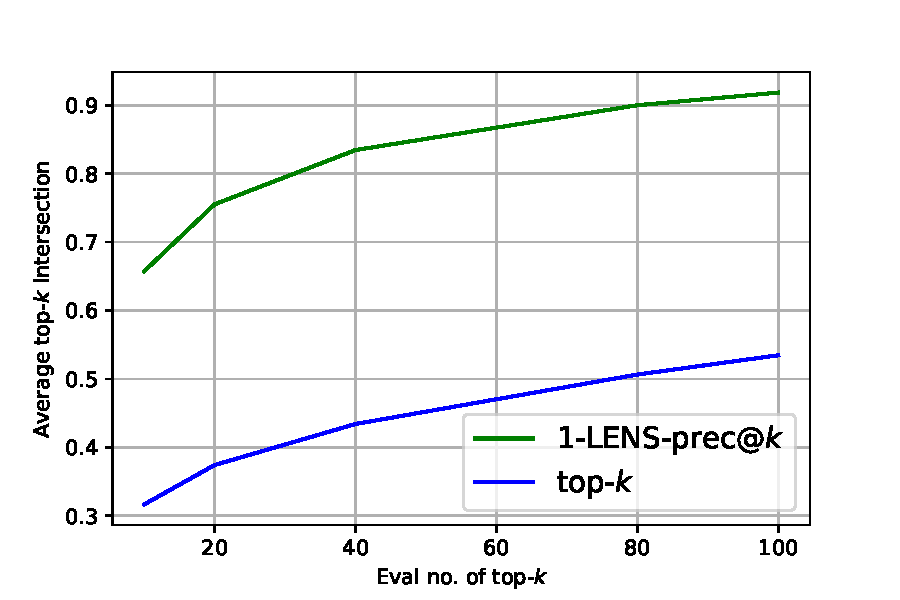
\includegraphics[width=1.0\textwidth]{./plots/gtsrb_topkvsrand_topk_nat.pdf}
    \caption{GTSRB: top-$k$}
    \label{mnist-rand-fig:c}
    \end{subfigure}
    \begin{subfigure}[b]{0.12\textwidth}
    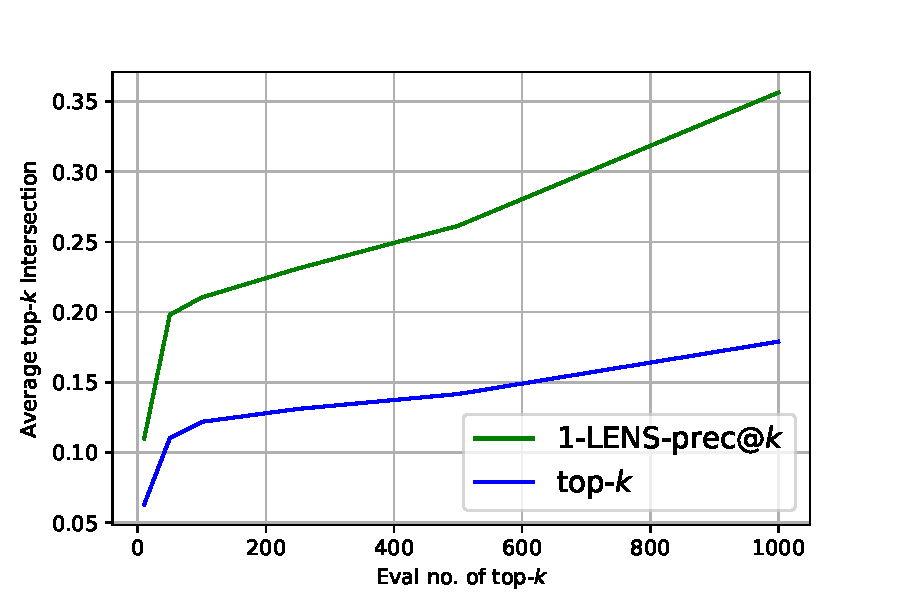
\includegraphics[width=1.0\textwidth]{./plots/flower_topkvsrand_3x3_topk_nat.pdf}
    \caption{Flower: top-$k$}
    \label{mnist-rand-fig:c}
    \end{subfigure}
    %\begin{subfigure}[b]{0.12\textwidth}
    %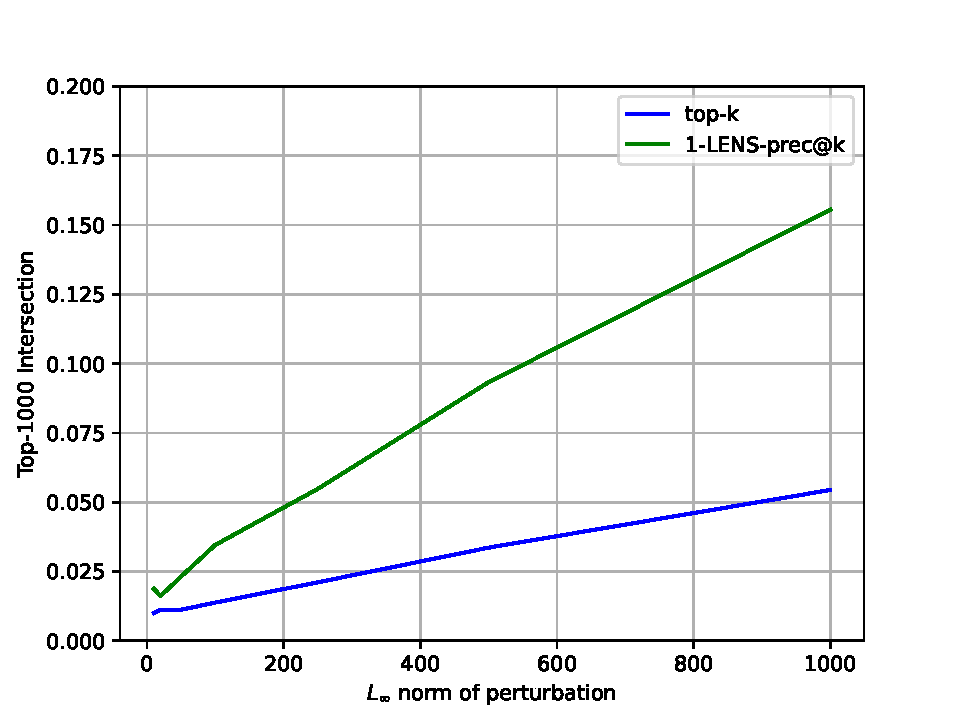
\includegraphics[width=1.0\textwidth]{./plots/imagenet_topkvsrand_3x3_topk_nat.pdf}
    %\caption{ImageNet: top-$t$}
    %\label{mnist-rand-fig:d}
    %\end{subfigure}
\end{subfigure}
\begin{subfigure}[b]{1.0\textwidth}
    \begin{subfigure}[b]{0.12\textwidth}
    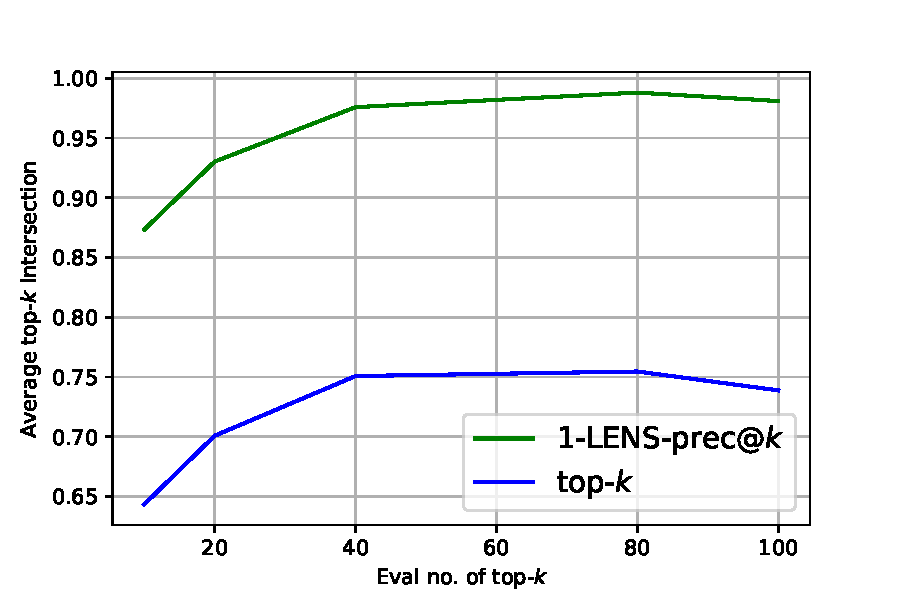
\includegraphics[width=1.0\textwidth]{./plots/mnist_topkvsrand_rand_nat.pdf}
    \caption{MNIST: random}
    \label{mnist-rand-fig:a}
    \end{subfigure}
    \begin{subfigure}[b]{0.12\textwidth}
    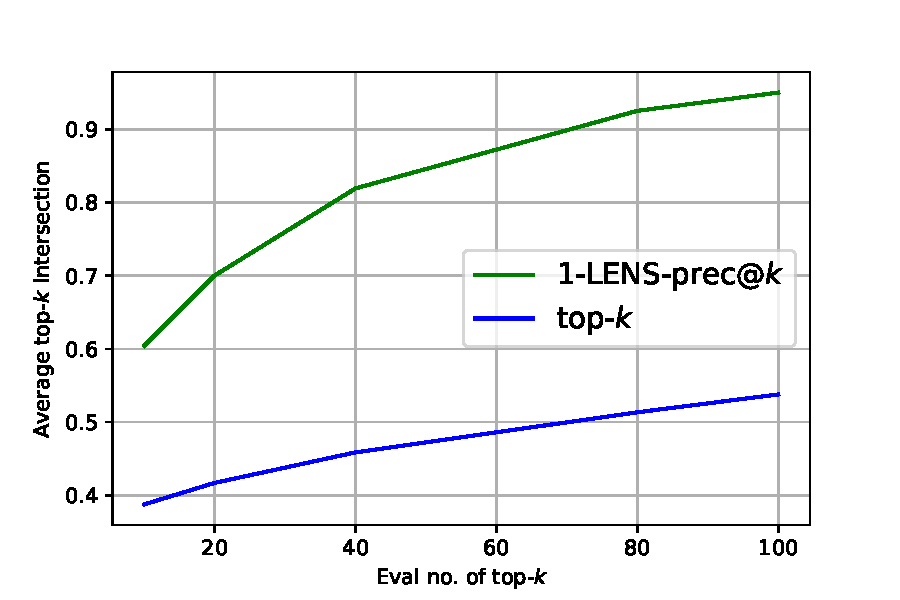
\includegraphics[width=1.0\textwidth]{./plots/fmnist_topkvsrand_rand_nat.pdf}
    \caption{F-MNIST: random}
    \label{mnist-rand-fig:b}
    \end{subfigure}
    \begin{subfigure}[b]{0.12\textwidth}
    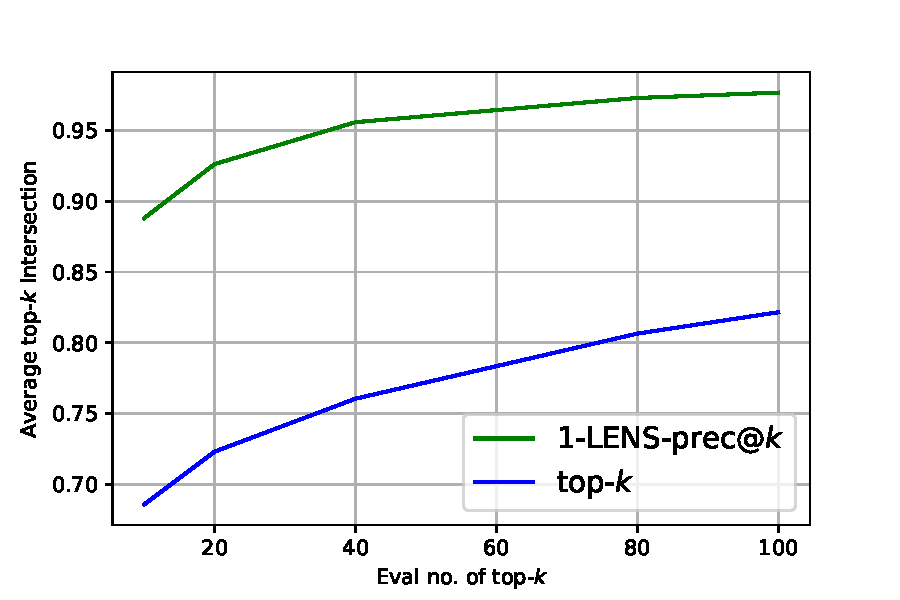
\includegraphics[width=1.0\textwidth]{./plots/gtsrb_topkvsrand_rand_nat.pdf}
    \caption{GTSRB: random}
    \label{mnist-rand-fig:c}
    \end{subfigure}
    \begin{subfigure}[b]{0.12\textwidth}
    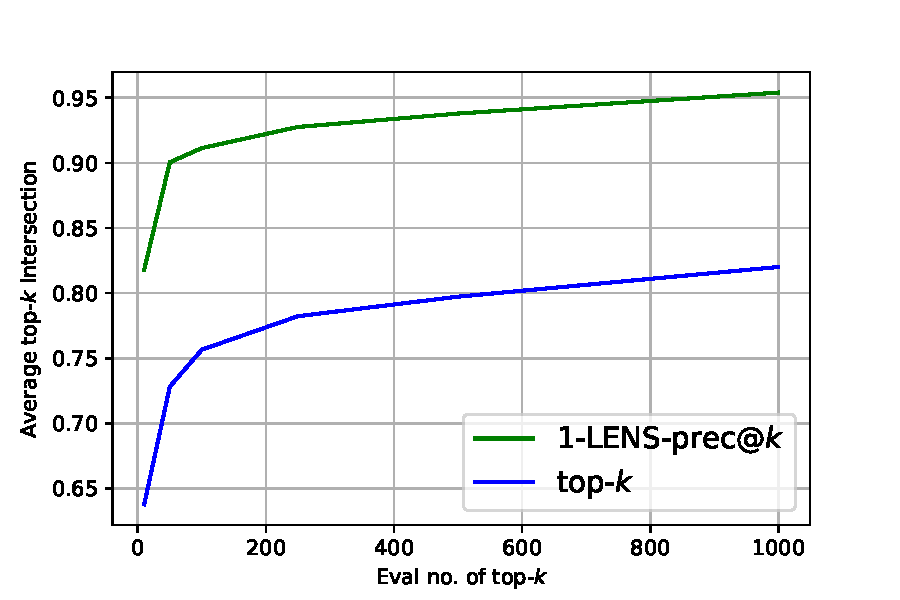
\includegraphics[width=1.0\textwidth]{./plots/flower_topkvsrand_3x3_rand_nat.pdf}
    \caption{Flower: random}
    \label{mnist-rand-fig:c}
    \end{subfigure}
    %\begin{subfigure}[b]{0.12\textwidth}
    %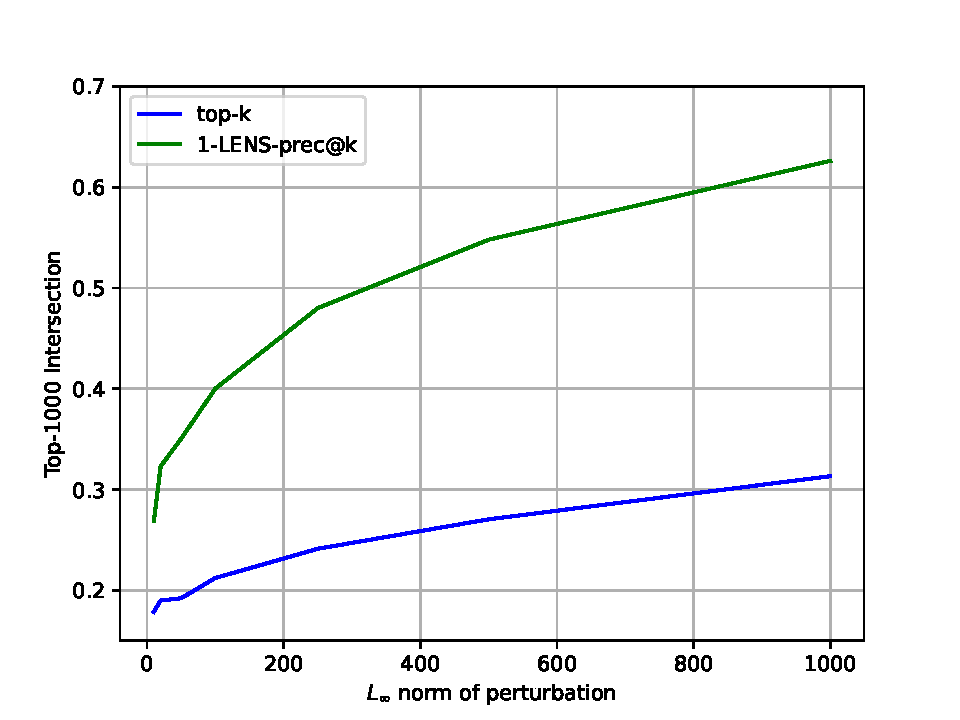
\includegraphics[width=1.0\textwidth]{./plots/imagenet_topkvsrand_3x3_rand_nat.pdf}
    %\caption{ImageNet: top-$t$}
    %\label{mnist-rand-fig:d}
    %\end{subfigure}
\end{subfigure}
\caption{Attributional robustness of IG on naturally trained models measured as average top-$k$ intersection and $1$-LENS-prec@$k$ between IG(original image) and IG(perturbed image). Perturbations are obtained by the {\bf top-$k$ attack} \citep{ghorbani2018interpretation} and random perturbation. The plots show how the above measures change with varying $k$ across different datasets.}
\label{dataset-topk-rand-diff-k-new-metric-nat}     
\end{figure}

\begin{figure}[!ht]
\centering
\begin{subfigure}[b]{1.0\textwidth}
    \begin{subfigure}[b]{0.12\textwidth}
    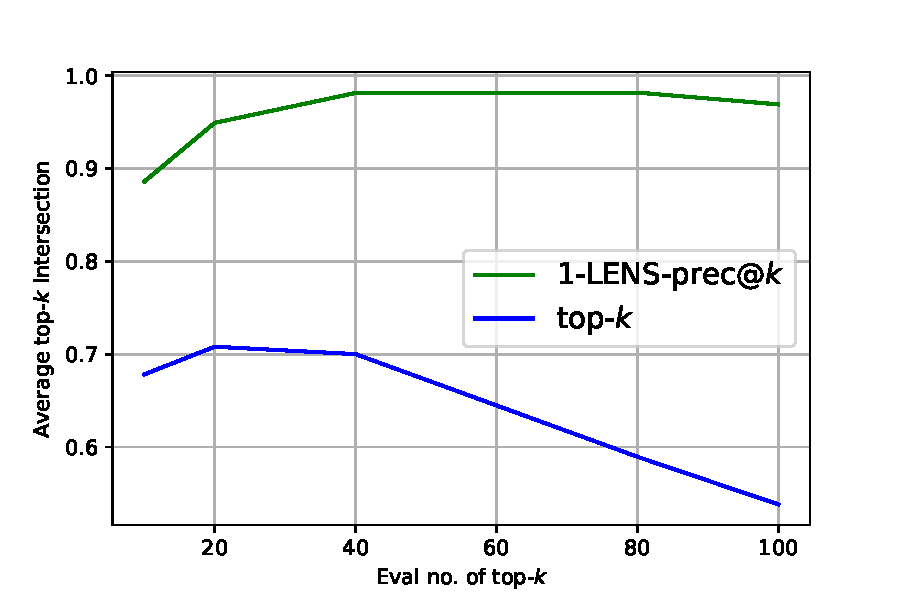
\includegraphics[width=1.0\textwidth]{./plots/mnist_topkvsrand_topk_pgd.pdf}
    \caption{MNIST IG : top-$k$}
    \label{mnist-rand-fig:a}
    \end{subfigure}
    \begin{subfigure}[b]{0.12\textwidth}
    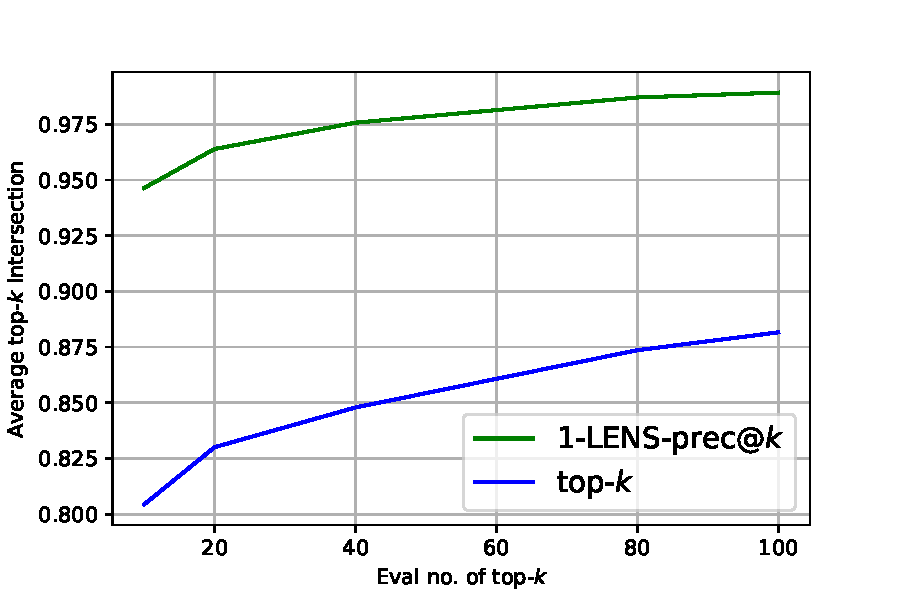
\includegraphics[width=1.0\textwidth]{./plots/fmnist_topkvsrand_topk_pgd.pdf}
    \caption{F-MNIST IG : top-$k$}
    \label{mnist-rand-fig:b}
    \end{subfigure}
    \begin{subfigure}[b]{0.12\textwidth}
    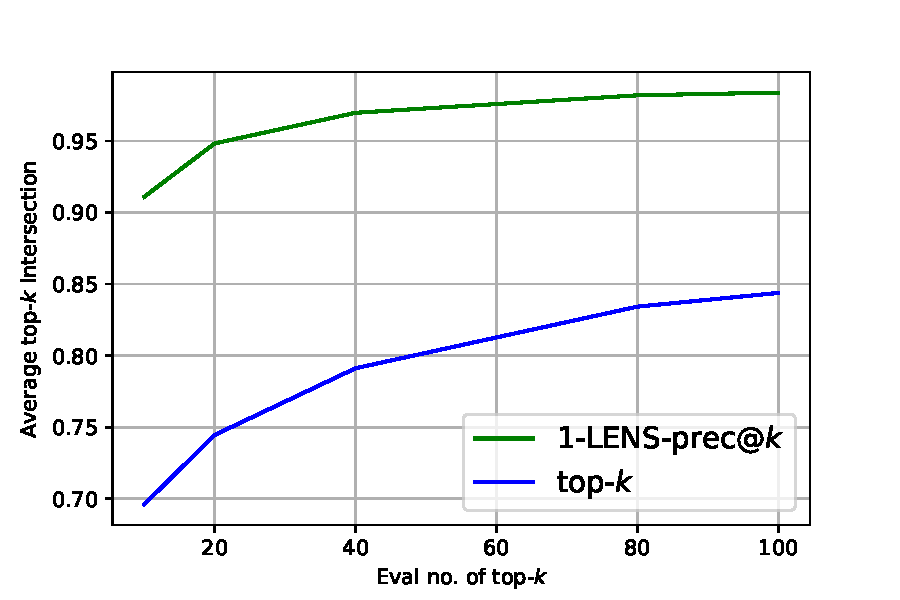
\includegraphics[width=1.0\textwidth]{./plots/gtsrb_topkvsrand_rand_pgd.pdf}
    \caption{GTSRB IG : top-$k$}
    \label{mnist-rand-fig:b}
    \end{subfigure}
    \begin{subfigure}[b]{0.12\textwidth}
    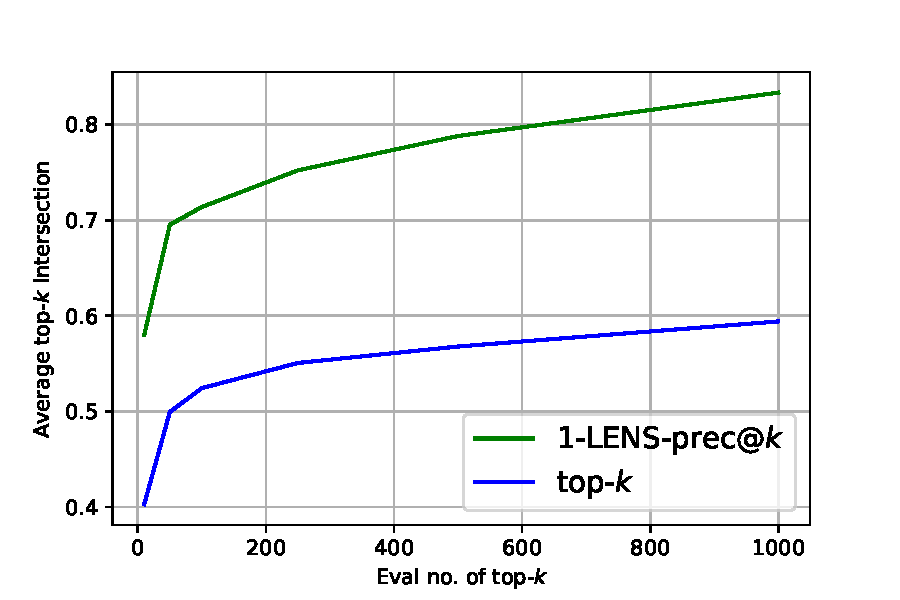
\includegraphics[width=1.0\textwidth]{./plots/flower_topkvsrand_3x3_topk_pgd.pdf}
    \caption{Flower IG : top-$k$}
    \label{mnist-rand-fig:c}
    \end{subfigure}
\end{subfigure}
\begin{subfigure}[b]{1.0\textwidth}
    \begin{subfigure}[b]{0.12\textwidth}
    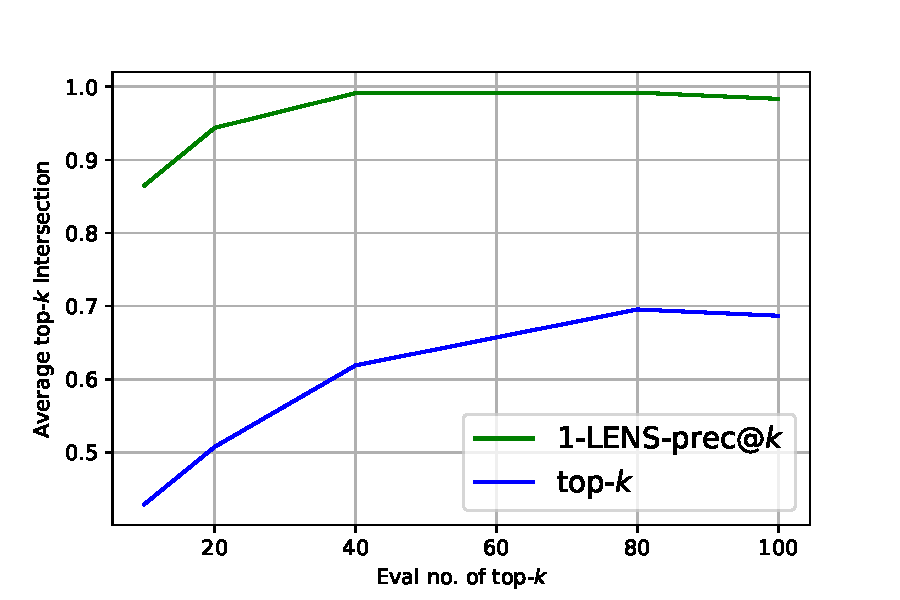
\includegraphics[width=1.0\textwidth]{./plots/mnist_topkvsrand_rand_pgd.pdf}
    \caption{MNIST IG : random}
    \label{mnist-rand-fig:a}
    \end{subfigure}
    \begin{subfigure}[b]{0.12\textwidth}
    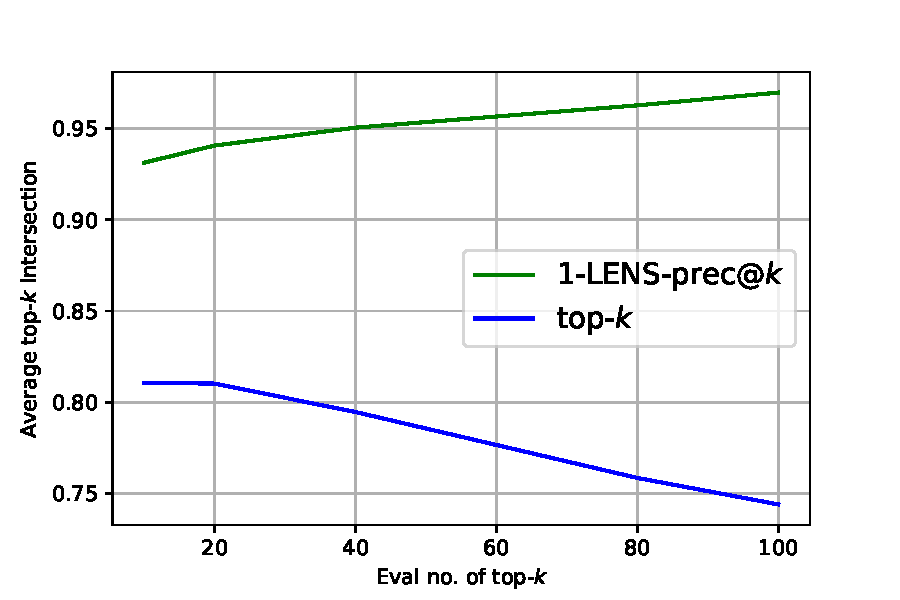
\includegraphics[width=1.0\textwidth]{./plots/fmnist_topkvsrand_rand_pgd.pdf}
    \caption{F-MNIST IG : random}
    \label{mnist-rand-fig:b}
    \end{subfigure}
    \begin{subfigure}[b]{0.12\textwidth}
    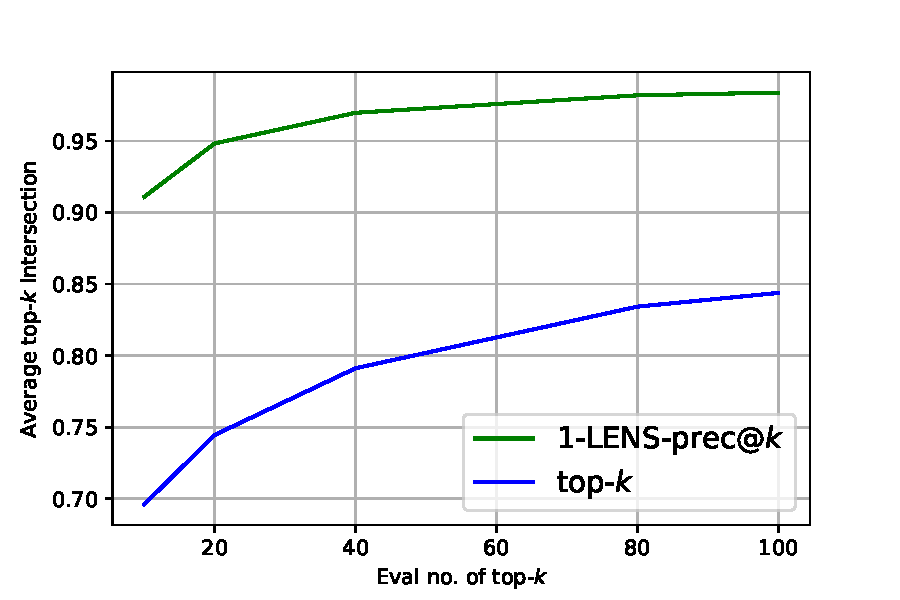
\includegraphics[width=1.0\textwidth]{./plots/gtsrb_topkvsrand_rand_pgd.pdf}
    \caption{GTSRB IG : random}
    \label{mnist-rand-fig:b}
    \end{subfigure}
    \begin{subfigure}[b]{0.12\textwidth}
    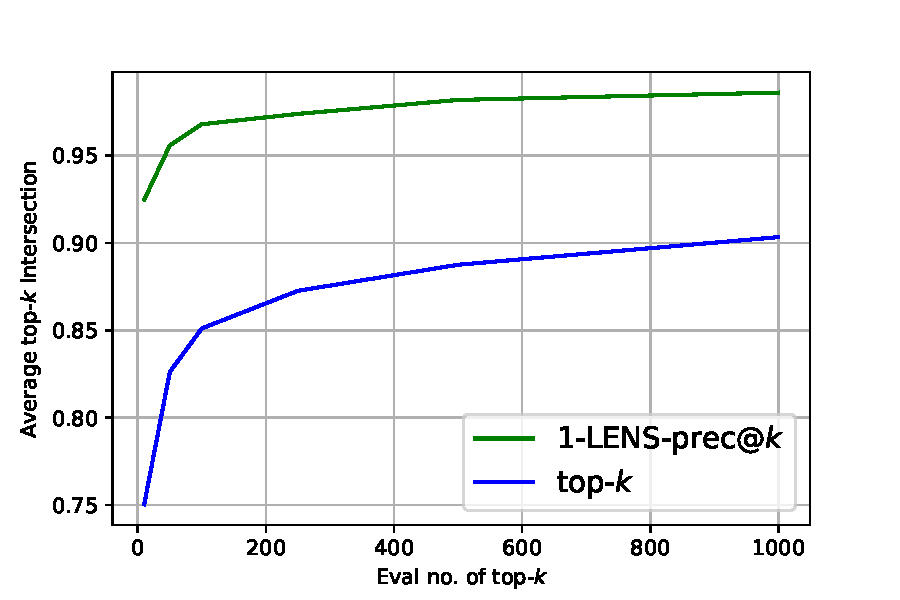
\includegraphics[width=1.0\textwidth]{./plots/flower_topkvsrand_3x3_rand_pgd.pdf}
    \caption{Flower IG : random}
    \label{mnist-rand-fig:c}
    \end{subfigure}
\end{subfigure}
\caption{Attributional robustness of IG on adversarially(PGD) trained models measured as average top-$k$ intersection and $1$-LENS-prec@$k$ between IG(original image) and IG(perturbed image). Perturbations are obtained by the {\bf top-$k$ attack} \citep{ghorbani2018interpretation} and random perturbation. The plots show how the above measures change with varying $k$ across different datasets.}
\label{dataset-topk-rand-diff-k-new-metric-pgd}  
\end{figure}

\begin{figure}[!ht]
\centering
\begin{subfigure}[b]{1.0\textwidth}
    \begin{subfigure}[b]{0.12\textwidth}
    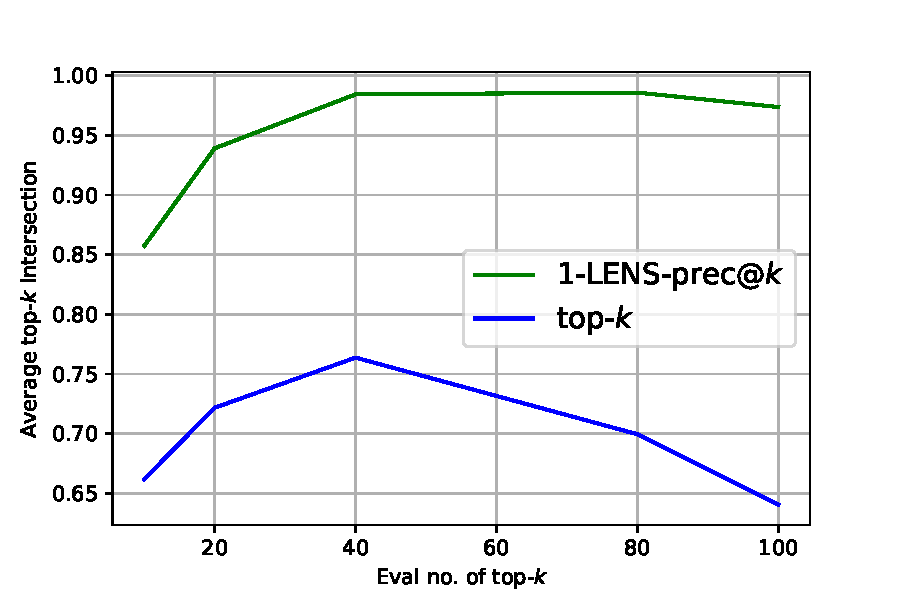
\includegraphics[width=1.0\textwidth]{./plots/mnist_topkvsrand_topk_rar.pdf}
    \caption{MNIST IG : top-$k$}
    \label{mnist-rand-fig:a}
    \end{subfigure}
    \begin{subfigure}[b]{0.12\textwidth}
    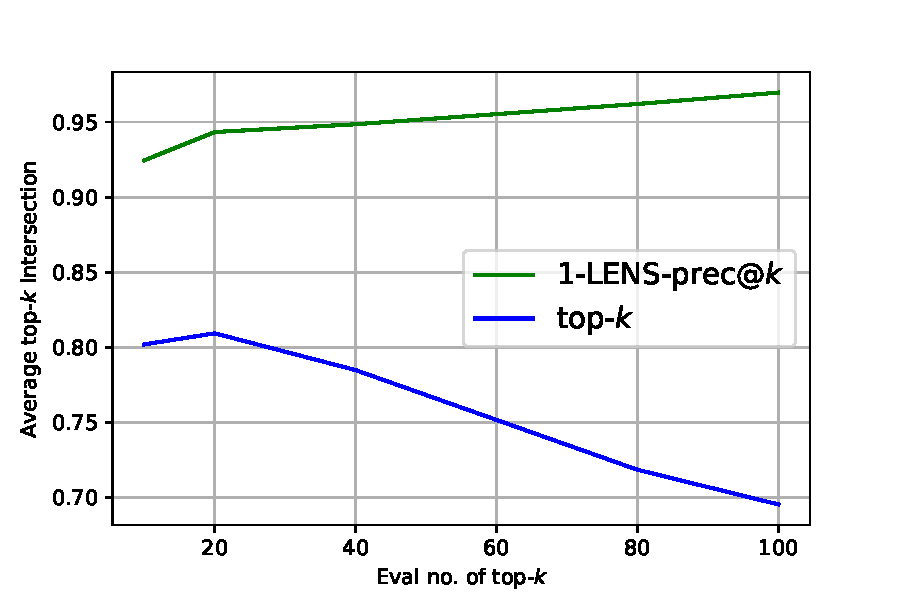
\includegraphics[width=1.0\textwidth]{./plots/fmnist_topkvsrand_topk_rar.pdf}
    \caption{F-MNIST IG : top-$k$}
    \label{mnist-rand-fig:b}
    \end{subfigure}
    \begin{subfigure}[b]{0.12\textwidth}
    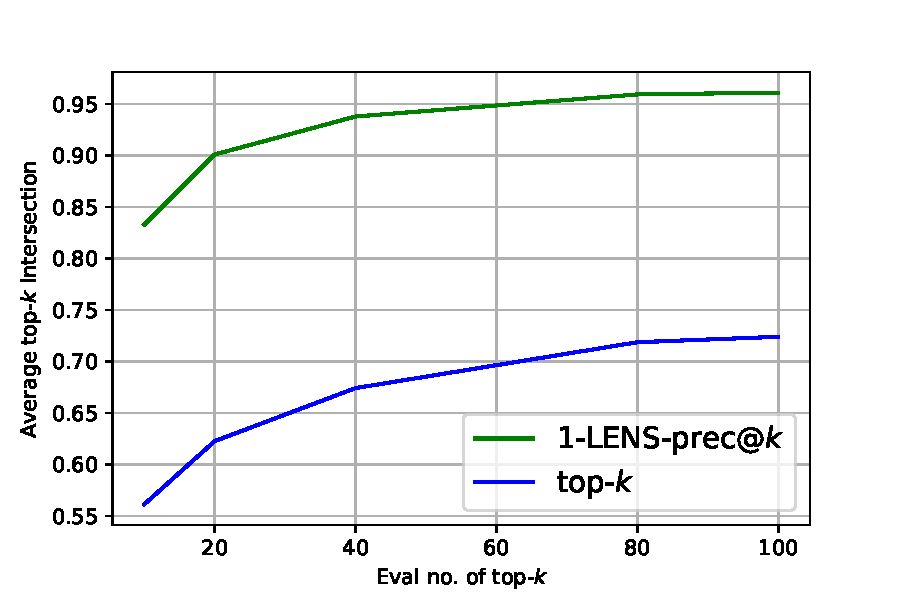
\includegraphics[width=1.0\textwidth]{./plots/gtsrb_topkvsrand_topk_rar.pdf}
    \caption{GTSRB IG : top-$k$}
    \label{mnist-rand-fig:b}
    \end{subfigure}
    \begin{subfigure}[b]{0.12\textwidth}
    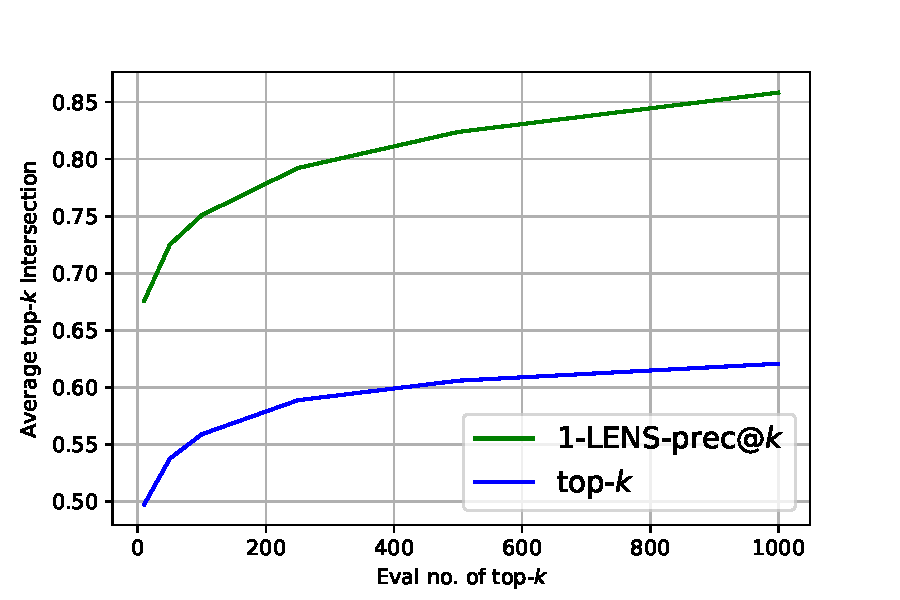
\includegraphics[width=1.0\textwidth]{./plots/flower_topkvsrand_3x3_topk_rar.pdf}
    \caption{Flower IG : top-$k$}
    \label{mnist-rand-fig:c}
    \end{subfigure}
\end{subfigure}
\begin{subfigure}[b]{1.0\textwidth}
    \begin{subfigure}[b]{0.12\textwidth}
    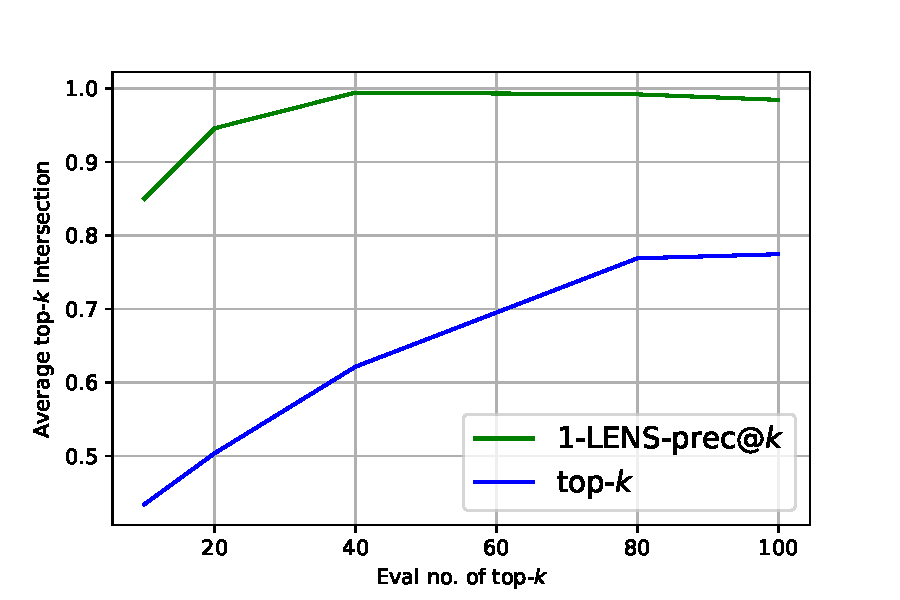
\includegraphics[width=1.0\textwidth]{./plots/mnist_topkvsrand_rand_rar.pdf}
    \caption{MNIST IG : random}
    \label{mnist-rand-fig:a}
    \end{subfigure}
    \begin{subfigure}[b]{0.12\textwidth}
    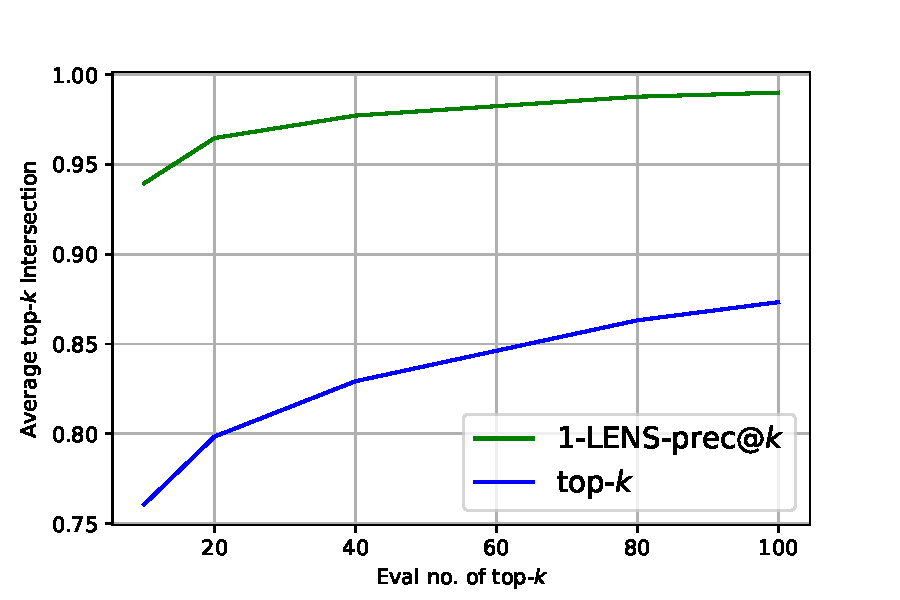
\includegraphics[width=1.0\textwidth]{./plots/fmnist_topkvsrand_rand_rar.pdf}
    \caption{F-MNIST IG : random}
    \label{mnist-rand-fig:b}
    \end{subfigure}
    \begin{subfigure}[b]{0.12\textwidth}
    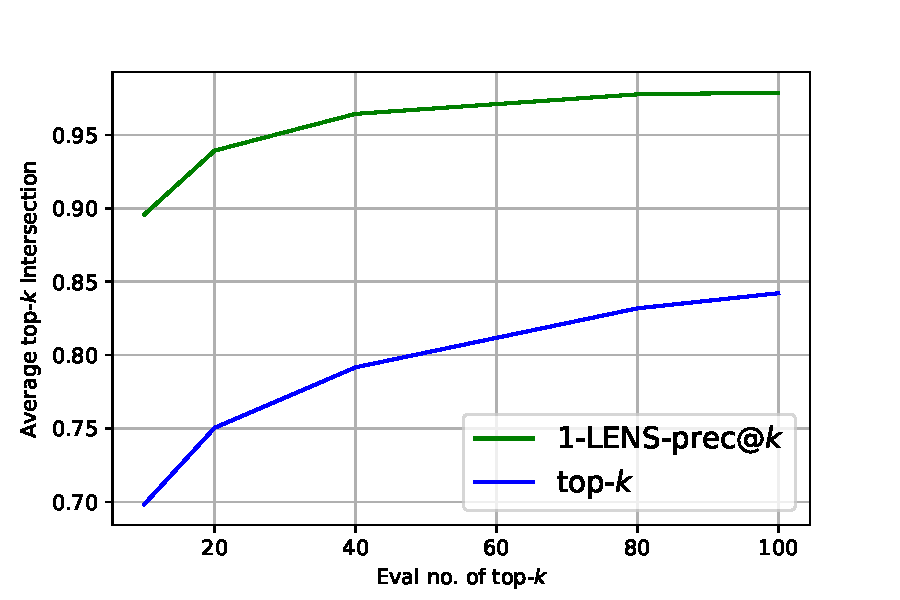
\includegraphics[width=1.0\textwidth]{./plots/gtsrb_topkvsrand_rand_rar.pdf}
    \caption{GTSRB IG : top-$k$}
    \label{mnist-rand-fig:b}
    \end{subfigure}
    \begin{subfigure}[b]{0.12\textwidth}
    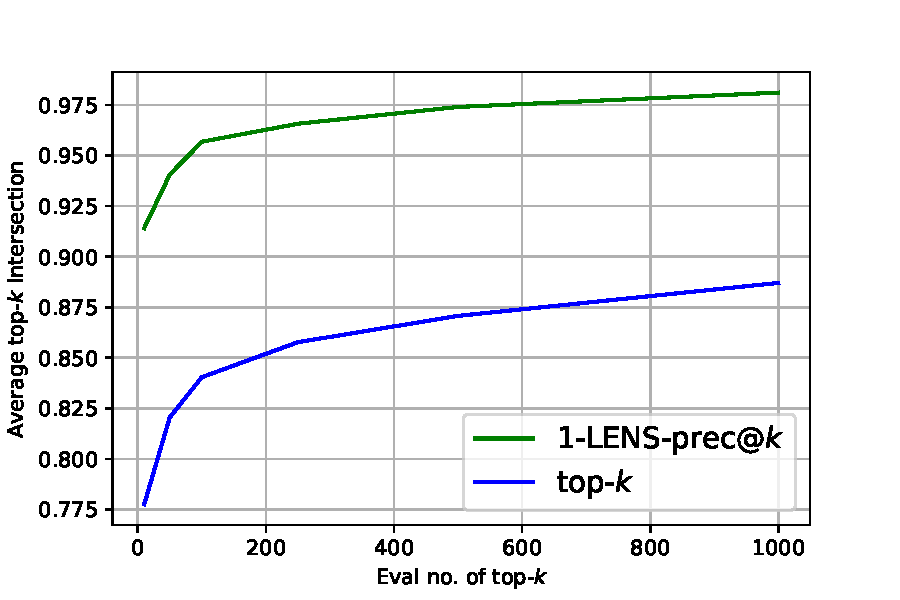
\includegraphics[width=1.0\textwidth]{./plots/flower_topkvsrand_3x3_rand_rar.pdf}
    \caption{Flower IG : random}
    \label{mnist-rand-fig:c}
    \end{subfigure}
\end{subfigure}
\caption{Attributional robustness of IG on IG-SUM-NORM trained models measured as average top-$k$ intersection and $1$-LENS-prec@$k$ between IG(original image) and IG(perturbed image). Perturbations are obtained by the {\bf top-$k$ attack} \citep{ghorbani2018interpretation} and random perturbation. The plots show how the above measures change with varying $k$ across different datasets.}
\label{dataset-topk-rand-diff-k-new-metric-rar}  
\end{figure}


\begin{figure}[!ht]
%\begin{wrapfigure}{r}{0.48\textwidth}
\centering
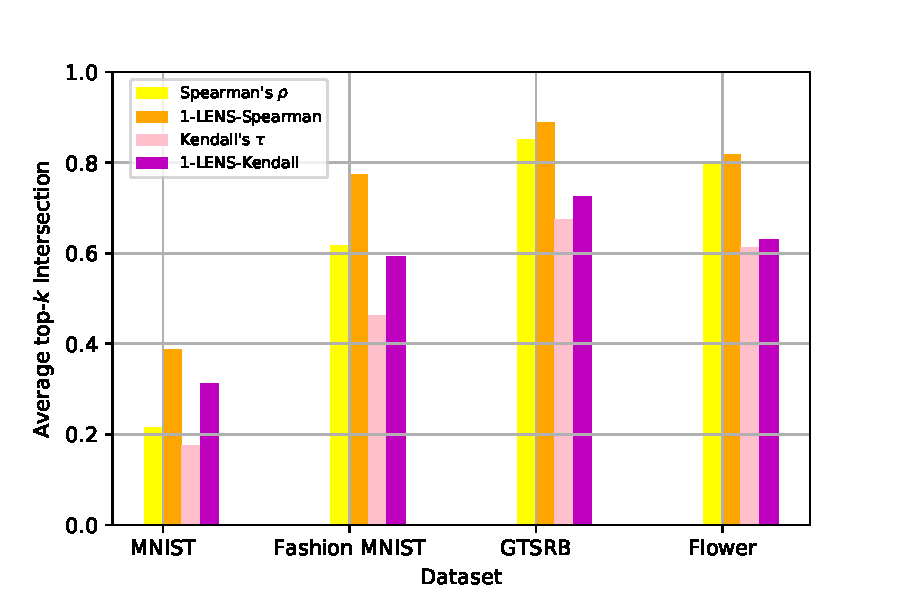
\includegraphics[width=0.38\textwidth]{./plots/datasets_mean_filter_3x3_metrics_notopk.pdf}
\caption{Attributional robustness of IG on naturally trained models measured as average Spearman's $\rho$, $1$-LENS-Spearman, Kendall $\tau$ and $1$-LENS-Kendall between IG(original image) and IG(perturbed image). The perturbations are obtained by the top-$t$ attack of \citet{ghorbani2018interpretation}.} 
\label{dataset-smooth-sp-ken-nat}
%\vspace{-5pt}
%\end{wrapfigure}
\end{figure}

\begin{figure}[!ht]
\centering
\begin{subfigure}[b]{\textwidth}
    \begin{subfigure}[b]{0.24\textwidth}
    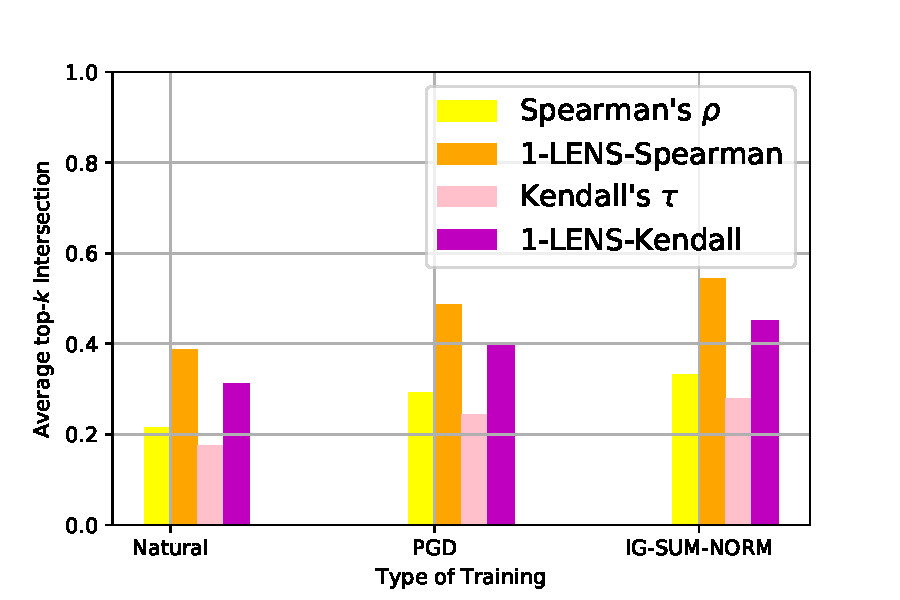
\includegraphics[width=\textwidth]{./plots/mnist_mean_filter_metrics_notopk.pdf}
    \caption{MNIST}
    \label{mnist-rand-fig:a}
    \end{subfigure}
    \begin{subfigure}[b]{0.24\textwidth}
    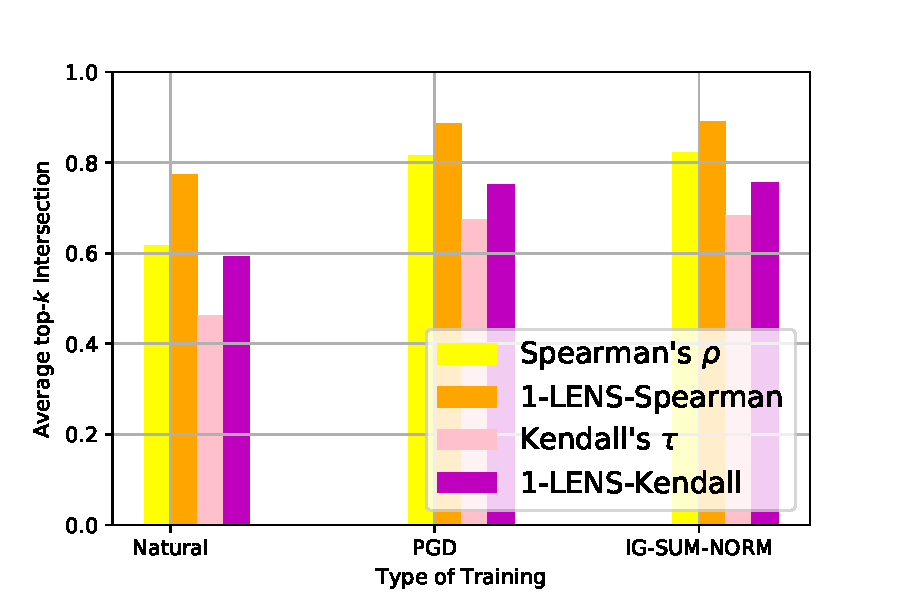
\includegraphics[width=\textwidth]{./plots/fmnist_mean_filter_metrics_notopk.pdf}
    \caption{Fashion MNIST}
    \label{fmnist-rand-fig:b}
    \end{subfigure}\\
    \begin{subfigure}[b]{0.24\textwidth}
    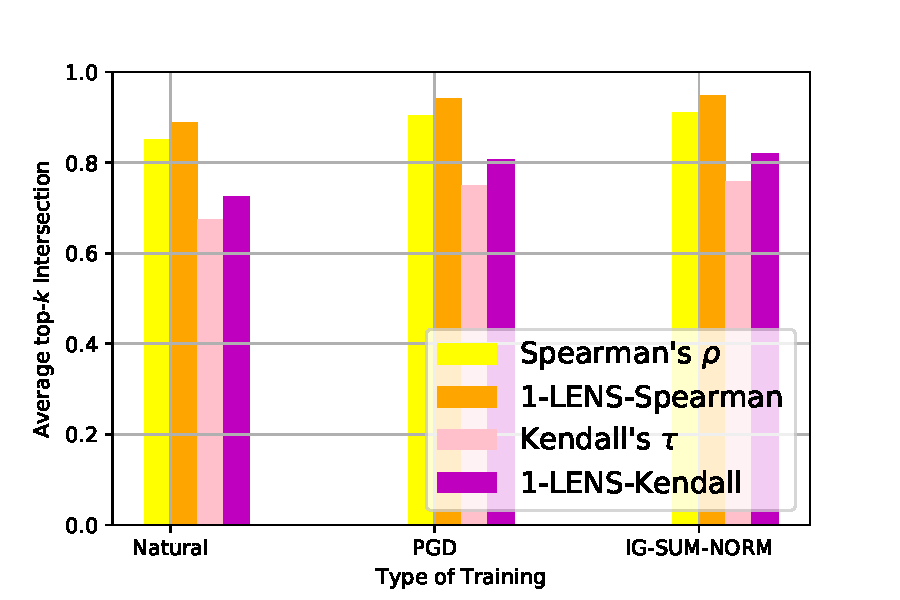
\includegraphics[width=\textwidth]{./plots/gtsrb_mean_filter_metrics_notopk.pdf}
    \caption{GTSRB}
    \label{gtsrb-rand-fig:c}
    \end{subfigure}
    \begin{subfigure}[b]{0.24\textwidth}
    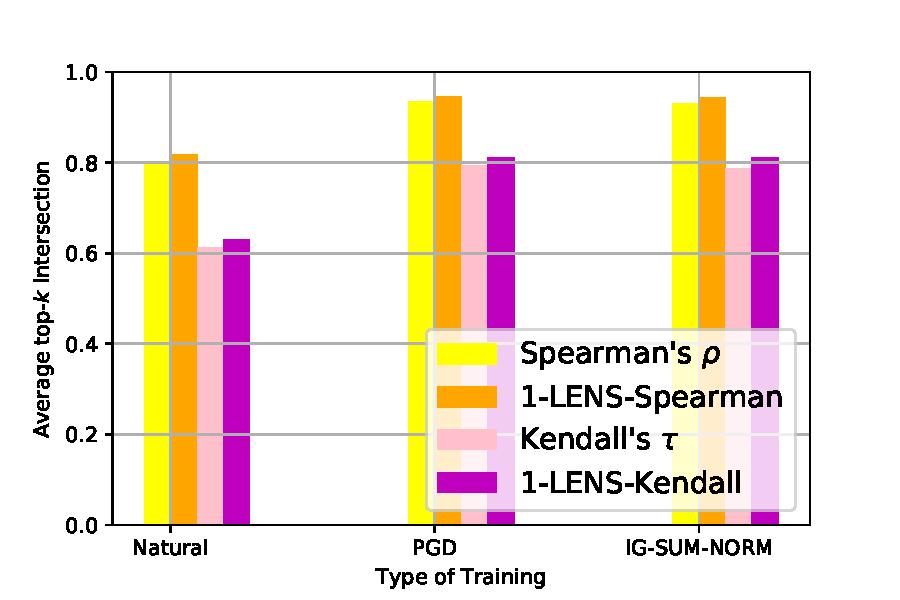
\includegraphics[width=\textwidth]{./plots/flower_mean_filter_3x3_metrics_notopk.pdf}
    \caption{Flower}
    \label{flower-rand-fig:d}
    \end{subfigure}
\end{subfigure}
\caption{Average Kendall's $\tau$, Spearman's $\rho$, $1$-LENS-Kendall and $1$-LENS-Spearman used to measure the attributional robustness of IG on natrually trained, PGD-trained and IG-SUM-NORM trained models. The perturbation used is the {\bf top-$k$ attack} of \citet{ghorbani2018interpretation}. Shown for (a) MNIST, (b) Fashion MNIST, (c) GTSRB and (d) Flower datasets.}
\label{dataset-smooth-sp-ken-nat-pgd-rar}   
\end{figure}

%\vspace{-5pt}
\paragraph{Comparison of Spearman's $\rho$ and Kendall's $\tau$ with $1$-LENS-Spearman and $1$-LENS-Kendall.} 
Figure \ref{dataset-smooth-sp-ken-nat} compares Spearman's $\rho$ and Kendall's $\tau$ with $1$-LENS-Spearman and $1$-LENS-Kendall measures for attributional robustness. We observe that $1$-smoothing of attribution maps increases the corresponding Kendall's $\tau$ and Spearman's $\rho$ measures of attributional robustness, and this observation holds across all datasets in our experiments. As a result, we believe that $1$-LENS-Spearman and $1$-LENS-Kendall result in better or tighter attributional robustness measures than Spearman's $\rho$ and Kendall's $\tau$. Additional results in Figure \ref{dataset-smooth-sp-ken-nat-pgd-rar}. 
%Spearman's $\rho$ and Kendall's $\tau$. We find that there is an improvement by using Spearman's and Kendall's rank correlation between mean smoothed IG maps. Each x-axis point is a trained network with the corresponding colored lines to be read in pairs. The pairs are using top-$k$, Spearman's $\rho$, Kendall's $\tau$ respectively before and after smoothing was applied. All datasets the same smoothing window of $3 \times 3$ was used.
%\begin{wrapfigure}{R}{0.4\textwidth}
%\begin{figure}[!ht]
%\centering
%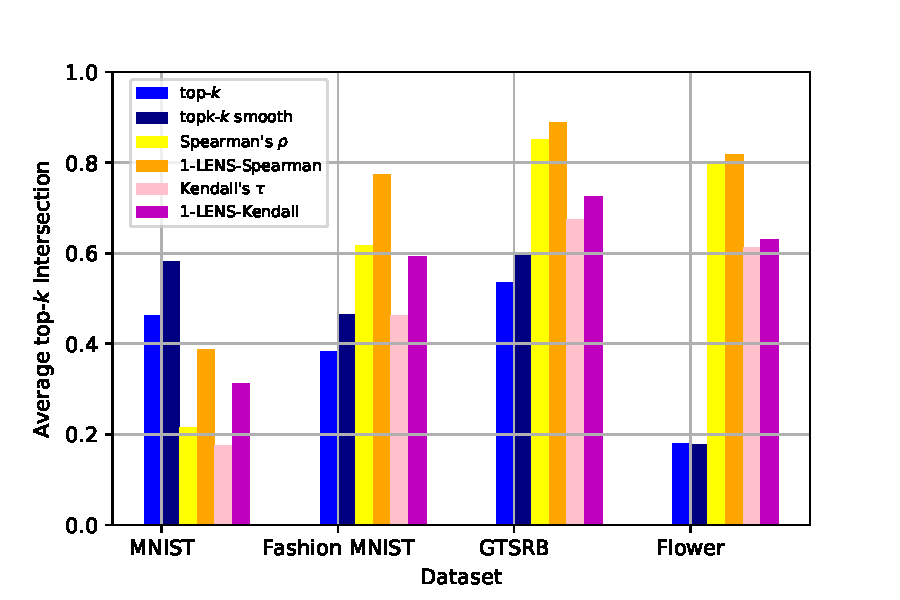
\includegraphics[width=0.4\textwidth]{./plots/datasets_mean_filter_3x3_metrics.pdf}
%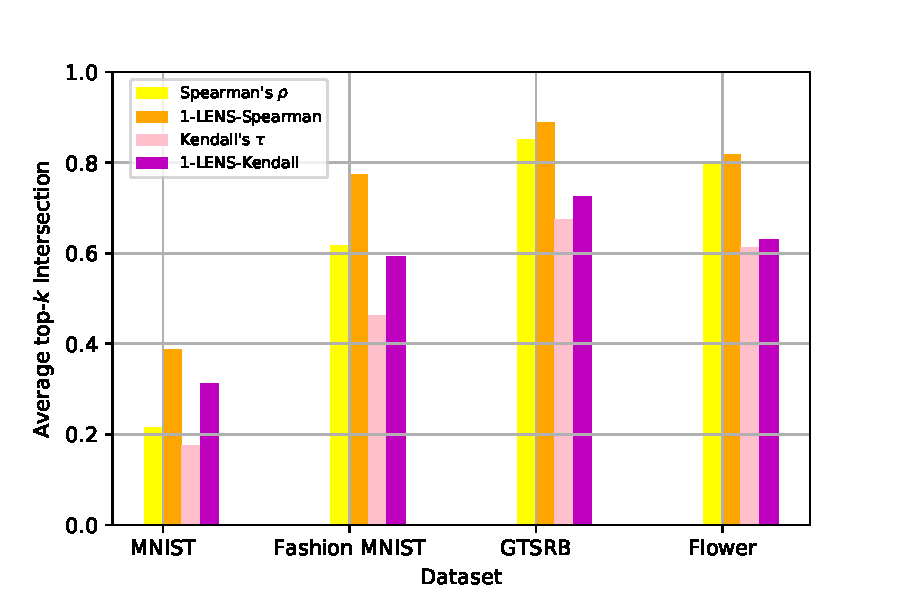
\includegraphics[width=0.4\textwidth]{./plots/datasets_mean_filter_3x3_metrics_notopk.pdf}
%\caption{Attributional robustness of IG on natural trained models measured as average Kendall $\tau$, $1$-LENS-Kendall, Spearman's $\rho$ and $1$-LENS-Spearman between IG(original image) and IG(perturbed image). The perturbations are obtained by the top-$t$ attack of \citet{ghorbani2018interpretation}.} 
%\label{dataset-smooth-sp-ken-nat}     
%\end{figure}
%\end{wrapfigure}

\paragraph{Modifying the attack of \citet{ghorbani2018interpretation} for $1$-LENS-prec@$k$ objective}

%\begin{figure}[!ht]
%\begin{wrapfigure}{r}{0.48\textwidth}
%\vspace{-15pt}
%\centering
%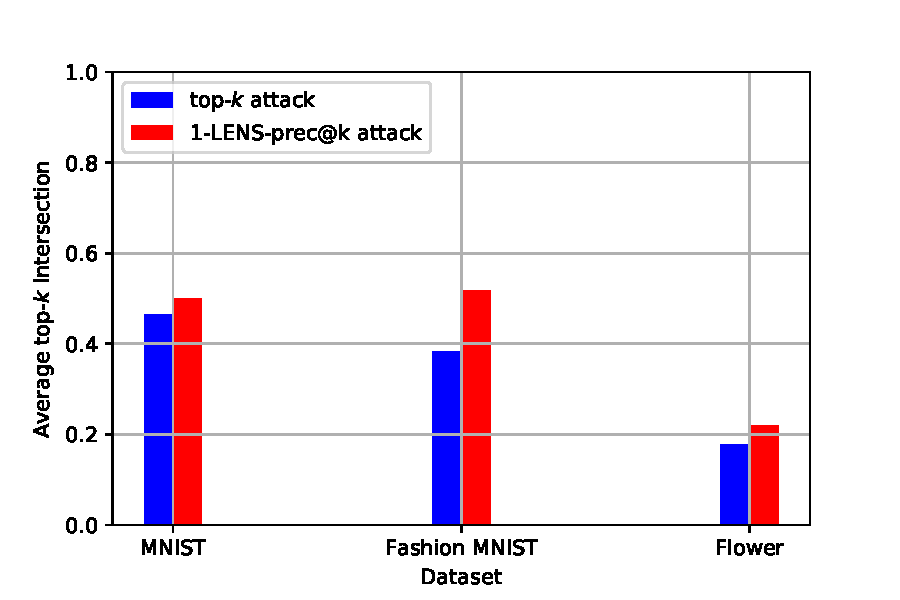
\includegraphics[width=0.33\textwidth]{./plots/dataset_gh3x3_topk_attack_old_metric.pdf}
%\caption{Average top-$k$ intersection between IG(original image) and IG(perturbed image) on naturally trained models where the perturbation is obtained by incorporating $1$-LENS-prec@$k$ objective in the \citet{ghorbani2018interpretation} attack.} 
%\label{gh-new-attack-topk}     
%\vspace{-5pt}
%\end{wrapfigure}
%\end{figure}

A natural question is whether the original top-$k$ attack of \citet{ghorbani2018interpretation} seem weaker under locality-senstitive robustness measures only because the attack was specifically constructed for a corresponding top-$k$ intersection objective. Since the construction of the attack in \citet{ghorbani2018interpretation} is modifiable for any similarity objective, we use $1$-LENS-prec@$k$ to construct a new attributional attack for $1$-LENS-prec@$k$ objective based on the $k \times k$ neighborhood of pixels. Surprisingly, we notice that it leads to a \emph{worse} attributional attack, if we measure its effectiveness using the top-$k$ intersection; see Figure \ref{app:modify-ghorbani-with-lens}. In other words, attributional attacks against locality-sensitive measures of attributional robustness are non-trivial and may require fundamentally different ideas.

\begin{figure}[!ht]
%\vspace{-12pt}
\centering
    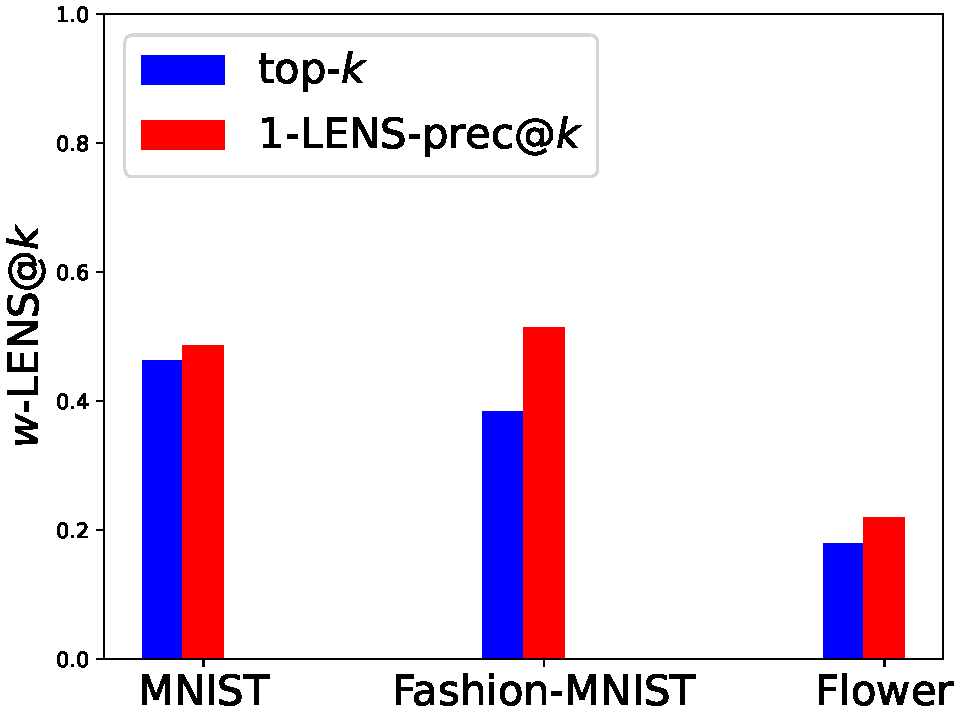
\includegraphics[width=0.24\textwidth]{./plots/dataset_gh3x3_topk_attack_old_metric_1.pdf}
    %\vspace{-6pt}
\caption{Average top-$k$ intersection between IG(original image) and IG(perturbed image) on naturally trained models where the perturbation is obtained by incorporating $1$-LENS-prec@$k$ objective in the \citet{ghorbani2018interpretation} attack.
} 
\label{app:modify-ghorbani-with-lens}
%\vspace{-20pt}
%\end{wrapfigure}
\end{figure}

%\clearpage 

\subsection{Experiments with Integrated Gradients} \label{app:all-ig-exp}
Below we present additional experimental results for Integrated Gradients (IG).
%\paragraph{Other Empirical Results for Section \ref{sec:ext-fragile}} \label{app:all-ig-exp:sec:ext-fragile}

\begin{figure}[!ht]
\centering
\begin{subfigure}[b]{\textwidth}
    \begin{subfigure}[b]{0.24\textwidth}
    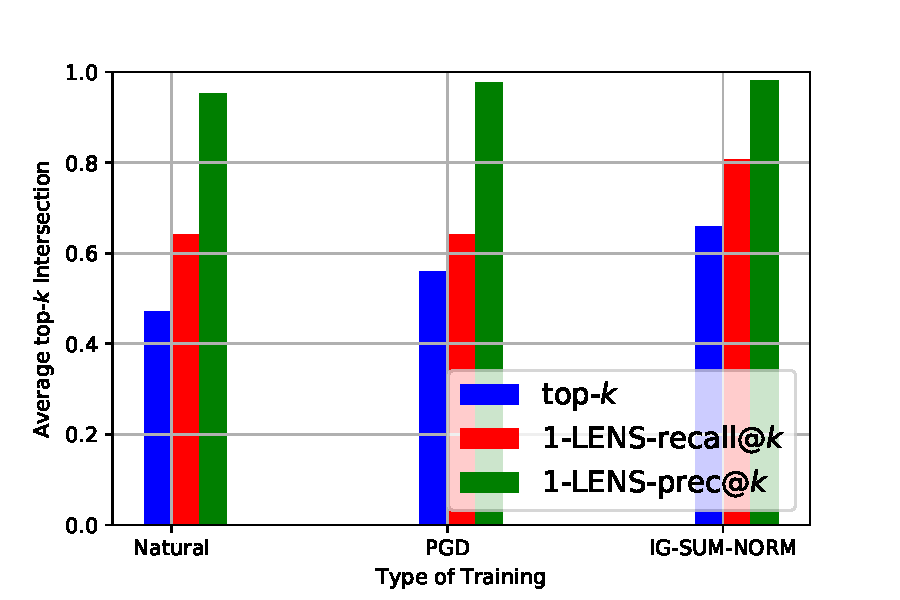
\includegraphics[width=\textwidth]{./plots/mnist_topk_attack_new_metric.pdf}
    \caption{MNIST}
    \label{mnist-rand-fig:a}
    \end{subfigure}
    \begin{subfigure}[b]{0.24\textwidth}
    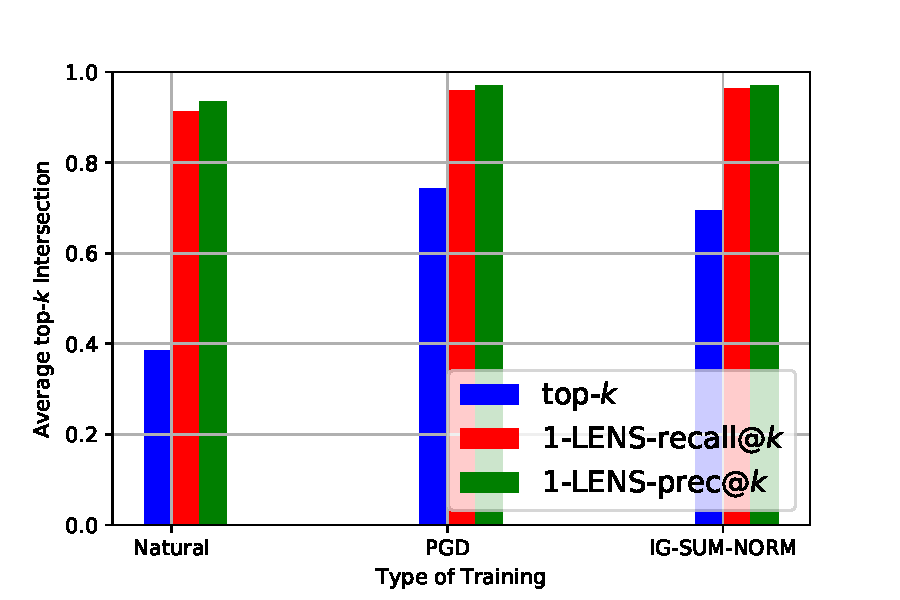
\includegraphics[width=\textwidth]{./plots/fmnist_topk_attack_new_metric.pdf}
    \caption{Fashion MNIST}
    \label{fmnist-rand-fig:b}
    \end{subfigure}\\
    \begin{subfigure}[b]{0.24\textwidth}
    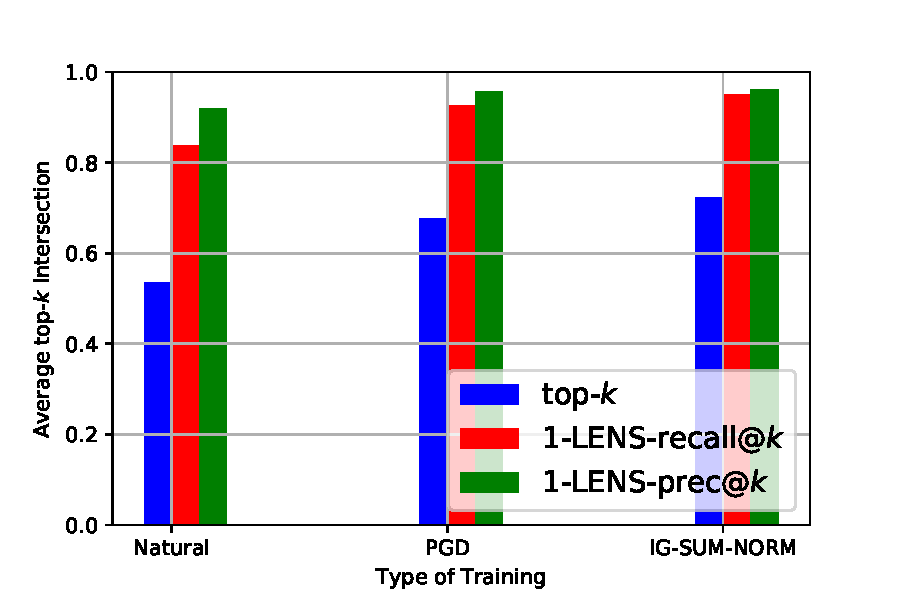
\includegraphics[width=\textwidth]{./plots/gtsrb_topk_attack_new_metric.pdf}
    \caption{GTSRB}
    \label{gtsrb-rand-fig:c}
    \end{subfigure}
    \begin{subfigure}[b]{0.24\textwidth}
    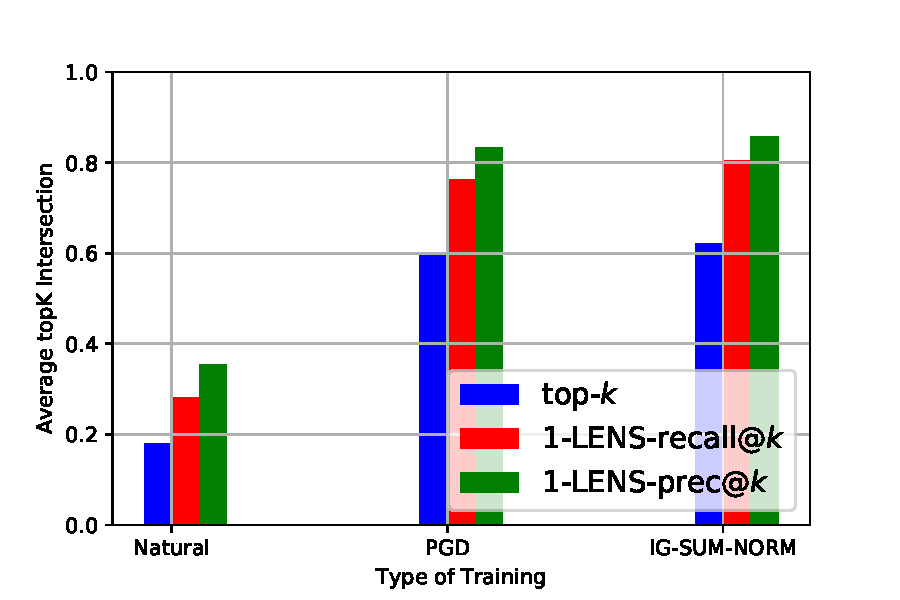
\includegraphics[width=\textwidth]{./plots/flower_topk_3x3_attack_new_metric.pdf}
    \caption{Flower}
    \label{flower-rand-fig:d}
    \end{subfigure}
\end{subfigure}
\caption{Average top-$k$ intersection, $1$-LENS-prec@$k$, $1$-LENS-recall@$k$ measured between IG(original image) and IG(perturbed image) for models that are naturally trained, PGD-trained and IG-SUM-NORM trained. The perturbation used is the {\bf top-$k$} attack of \cite{ghorbani2018interpretation}. Shown for (a) MNIST, (b) Fashion MNIST, (c) GTSRB and (d) Flower datasets.}
\label{dataset-topk-new-metric-st-nat-pgd-rar}     
\end{figure}

\begin{figure}[!ht]
\centering
\begin{subfigure}[b]{1.0\textwidth}
    \begin{subfigure}[b]{0.24\textwidth}
    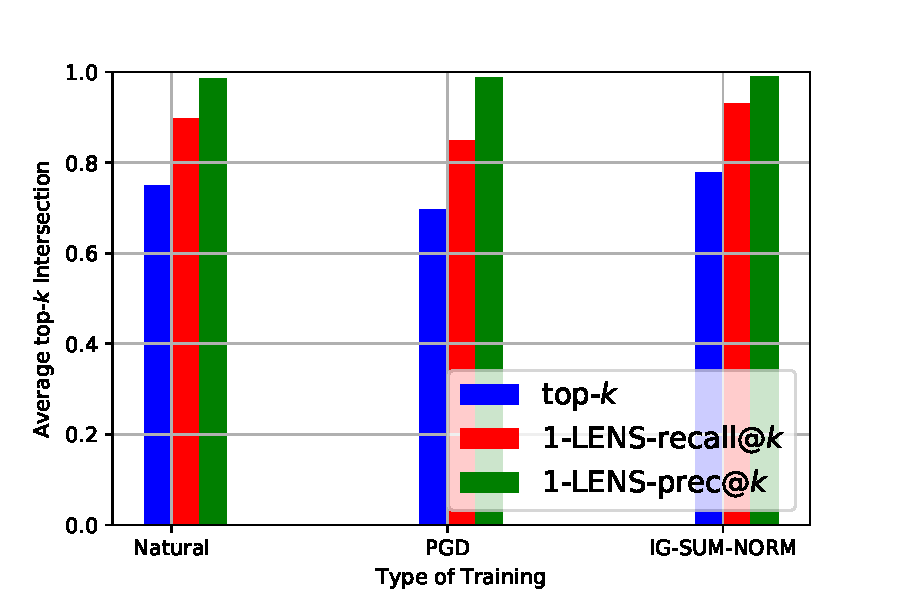
\includegraphics[width=1.0\textwidth]{./plots/mnist_random_attack_new_metric.pdf}
    \caption{MNIST}
    \label{mnist-rand-fig:a}
    \end{subfigure}
    \begin{subfigure}[b]{0.24\textwidth}
    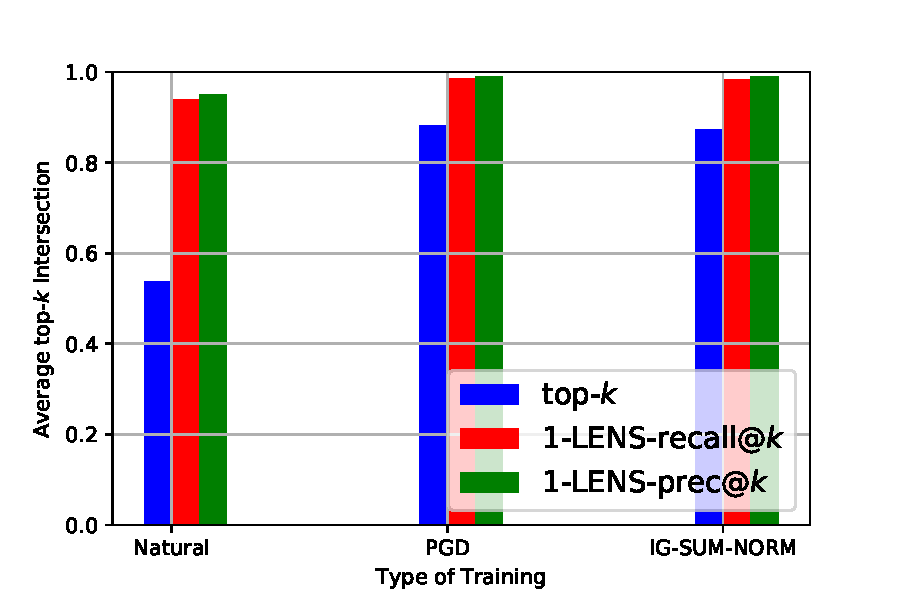
\includegraphics[width=1.0\textwidth]{./plots/fmnist_random_attack_new_metric.pdf}
    \caption{Fashion MNIST}
    \label{fmnist-rand-fig:b}
    \end{subfigure}\\
    \begin{subfigure}[b]{0.24\textwidth}
    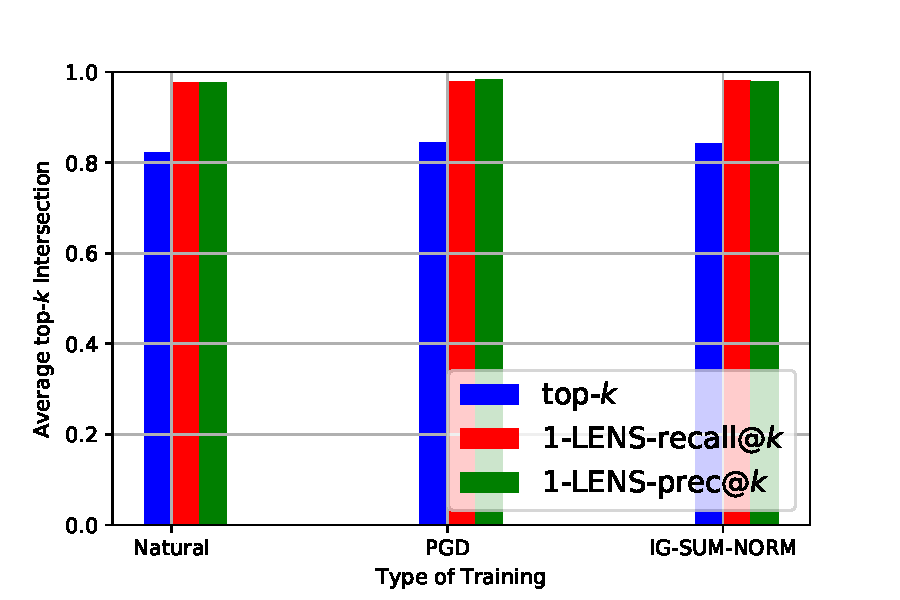
\includegraphics[width=1.0\textwidth]{./plots/gtsrb_random_attack_new_metric.pdf}
    \caption{GTSRB}
    \label{gtsrb-rand-fig:c}
    \end{subfigure}
    \begin{subfigure}[b]{0.24\textwidth}
    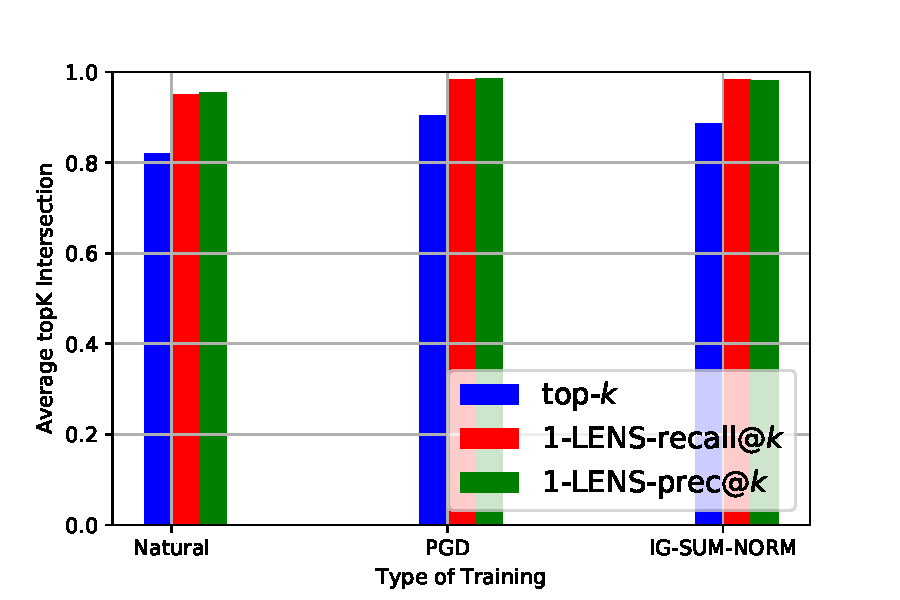
\includegraphics[width=1.0\textwidth]{./plots/flower_random_3x3_attack_new_metric.pdf}
    \caption{Flower}
    \label{flower-rand-fig:d}
    \end{subfigure}
\end{subfigure}
\caption{Attributional robustness of IG on naturally, PGD and IG-SUM-NORM trained models measured as top-$k$ intersection, $1$-LENS-prec@$k$ and $1$-LENS-recall@$k$ between the IG of the original images and the IG of their perturbations obtained by the {\bf random sign} attack \citep{ghorbani2018interpretation} across different datasets.} 
\label{rand-new-metric-training-method}     
\end{figure}

\begin{figure}[!ht]
\centering
\begin{subfigure}[b]{1.0\textwidth}
    \begin{subfigure}[b]{0.24\textwidth}
    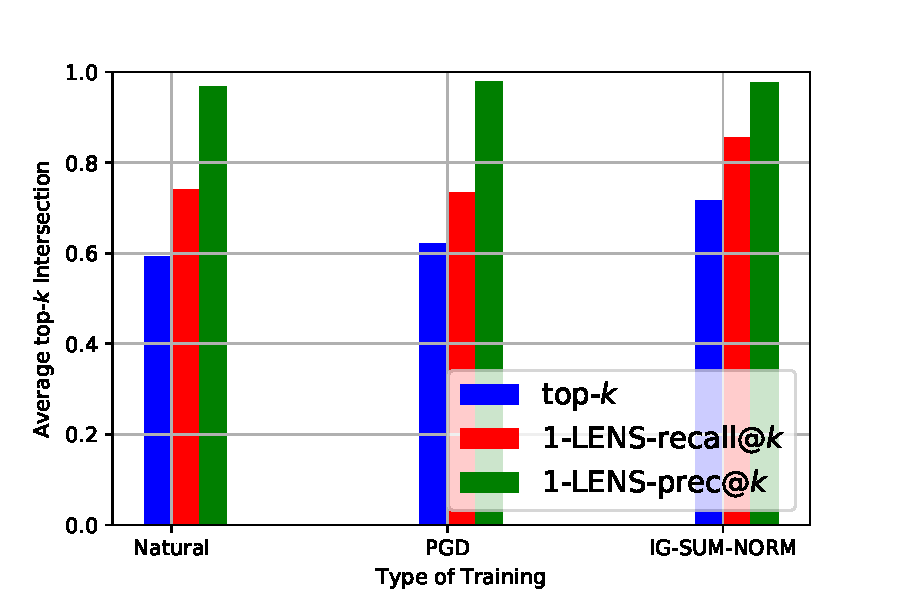
\includegraphics[width=1.0\textwidth]{./plots/mnist_mc_attack_new_metric.pdf}
    \caption{MNIST}
    \label{mnist-rand-fig:a}
    \end{subfigure}
    \begin{subfigure}[b]{0.24\textwidth}
    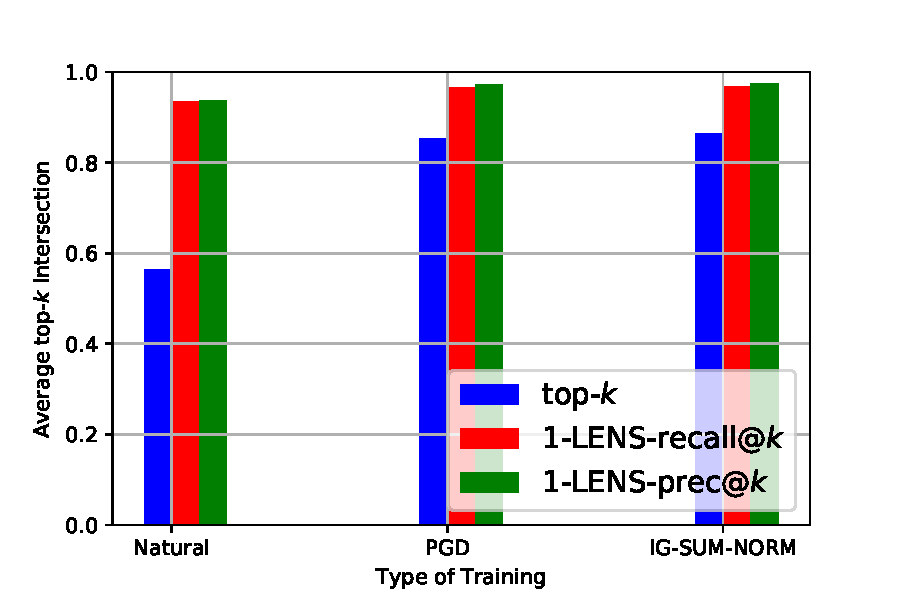
\includegraphics[width=1.0\textwidth]{./plots/fmnist_mc_attack_new_metric.pdf}
    \caption{Fashion MNIST}
    \label{fmnist-rand-fig:b}
    \end{subfigure}\\
    \begin{subfigure}[b]{0.24\textwidth}
    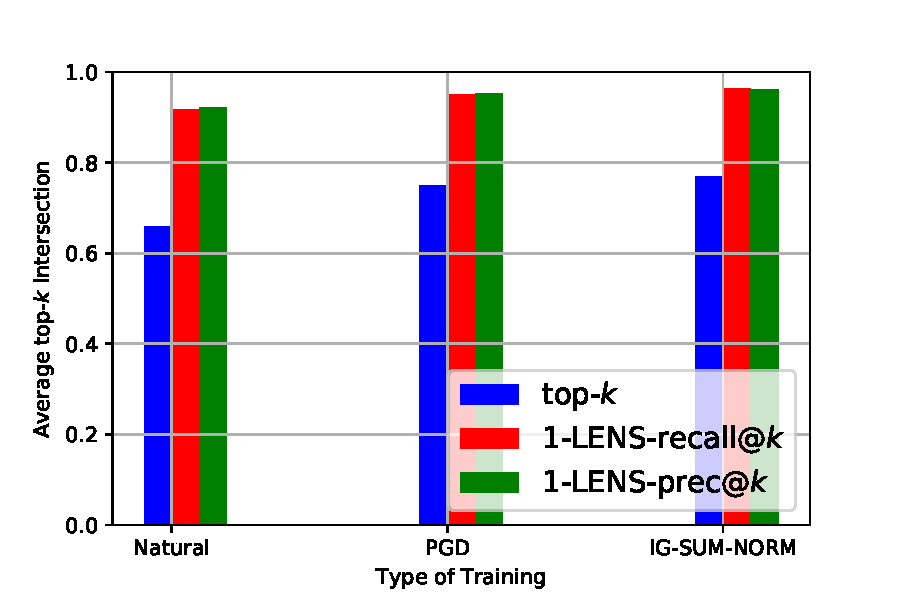
\includegraphics[width=1.0\textwidth]{./plots/gtsrb_mc_attack_new_metric.pdf}
    \caption{GTSRB}
    \label{gtsrb-rand-fig:c}
    \end{subfigure}
    \begin{subfigure}[b]{0.24\textwidth}
    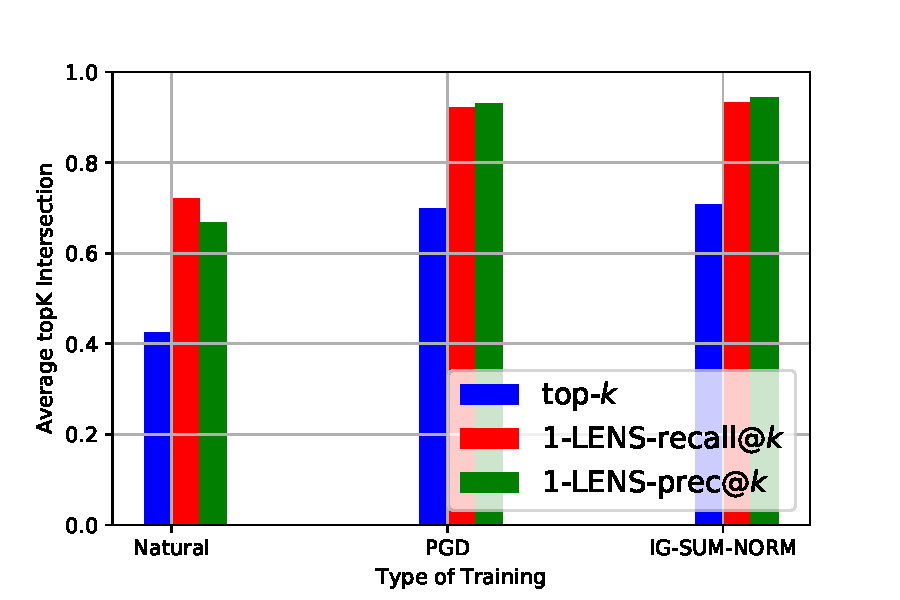
\includegraphics[width=1.0\textwidth]{./plots/flower_mc_3x3_attack_new_metric.pdf}
    \caption{Flower}
    \label{flower-rand-fig:d}
    \end{subfigure}
\end{subfigure}
\caption{Attributional robustness of IG on naturally, PGD and IG-SUM-NORM trained models measured as top-$k$ intersection, $1$-LENS-prec@$k$ and $1$-LENS-recall@$k$ between the IG of the original images and the IG of their perturbations obtained by the {\bf mass center} attack \citep{ghorbani2018interpretation} across different datasets.} 
\label{mc-new-metric-training-method}     
\end{figure}

%\paragraph{Other Empirical Results for Section \ref{sec:lens}} \label{app:all-ig-exp:sec:lens}
%\paragraph{Other Empirical Results for Section \ref{sec:adv-robust}} \label{app:all-ig-exp:sec:sec:adv-robust}

\begin{figure}[!ht]
\centering
\begin{subfigure}[b]{1.0\textwidth}
    \begin{subfigure}[b]{0.24\textwidth}
    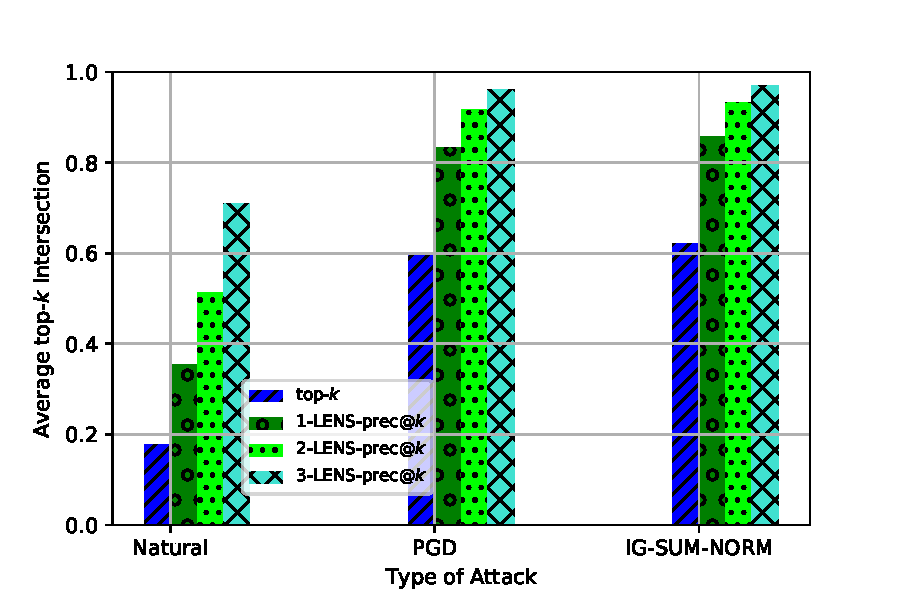
\includegraphics[width=1.0\textwidth]{./plots/flower_topk_attack_new_metric_ig.pdf}
    \caption{IG : top-$k$}
    \label{mnist-rand-fig:a}
    \end{subfigure}
    \begin{subfigure}[b]{0.24\textwidth}
    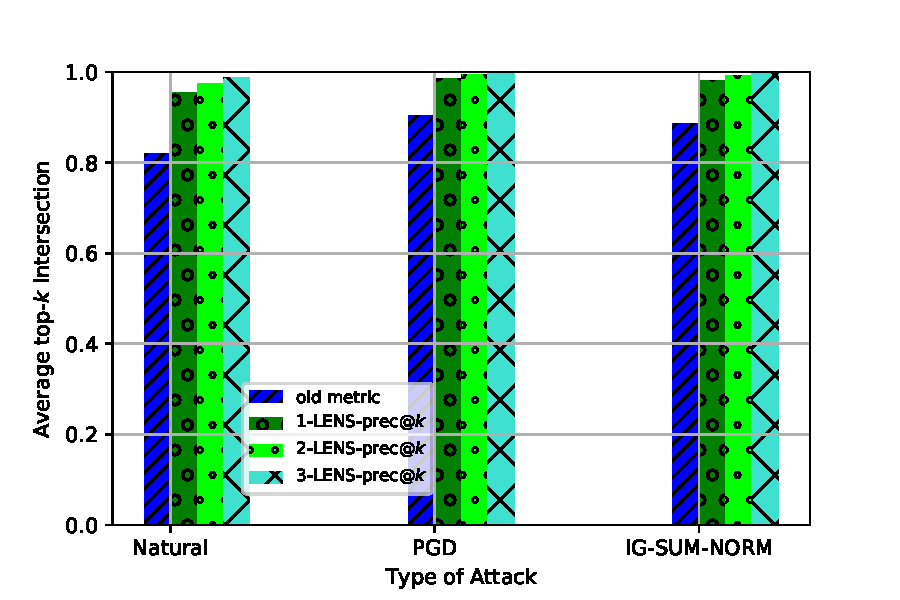
\includegraphics[width=1.0\textwidth]{./plots/flower_random_attack_new_metric_ig.pdf}
    \caption{IG : random}
    \label{mnist-rand-fig:b}
    \end{subfigure}\\
    \begin{subfigure}[b]{0.24\textwidth}
    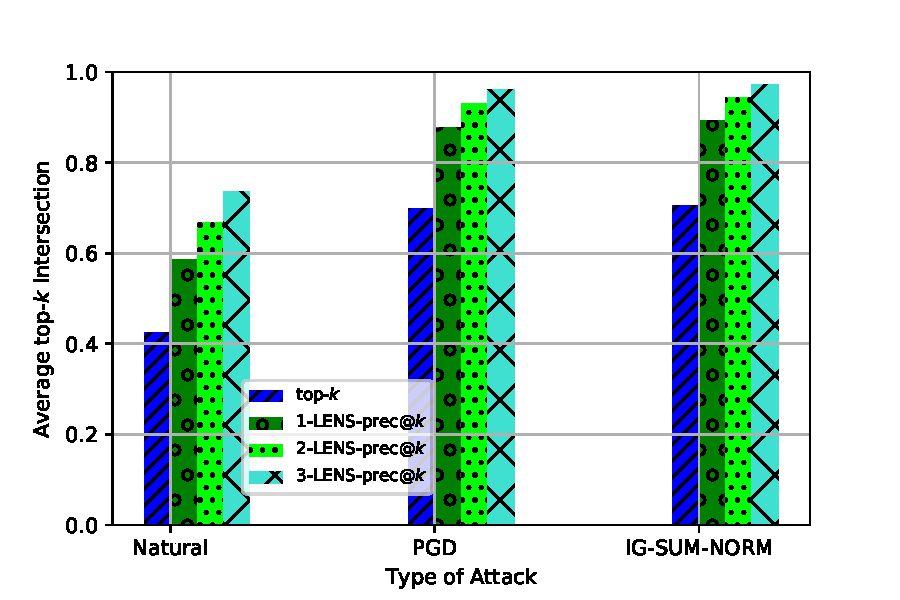
\includegraphics[width=1.0\textwidth]{./plots/flower_mc_attack_new_metric_ig.pdf}
    \caption{IG : center of mass}
    \label{mnist-rand-fig:c}
    \end{subfigure}
\end{subfigure}
\caption{Attributional robustness of IG on naturally, PGD and IG-SUM-NORM trained models measured as top-$k$ intersection and $w$-LENS-prec@$k$ between the IG of the original images and the IG of their perturbations. Perturbations are obtained by the top-$k$ attack and the mass center attack \citep{ghorbani2018interpretation} as well as a random perturbation. The plots show the effect of varying $w$ on Flower dataset.}
\label{flower-topk-new-metric-training-method}     
\end{figure}

\clearpage

\subsection{Experiments with Simple Gradients} \label{app:all-sg-exp}
We observe that our conclusions about Integrated Gradients (IG) continue to hold qualitatively, even if we replace IG with Simple Gradients as our attribution method.
%\paragraph{Other Empirical Results for Section \ref{sec:ext-fragile}} \label{app:all-sg-exp:sec:ext-fragile}
%\paragraph{Other Empirical Results for Section \ref{sec:lens} and \ref{sec:adv-robust}} \label{app:all-sg-exp:sec:lens}
%\paragraph{Other Empirical Results for Section \ref{sec:adv-robust}} \label{app:all-sg-exp:sec:sec:adv-robust}

\begin{figure}[!ht]
\centering
\begin{subfigure}[b]{1.0\textwidth}
    \begin{subfigure}[b]{0.24\textwidth}
    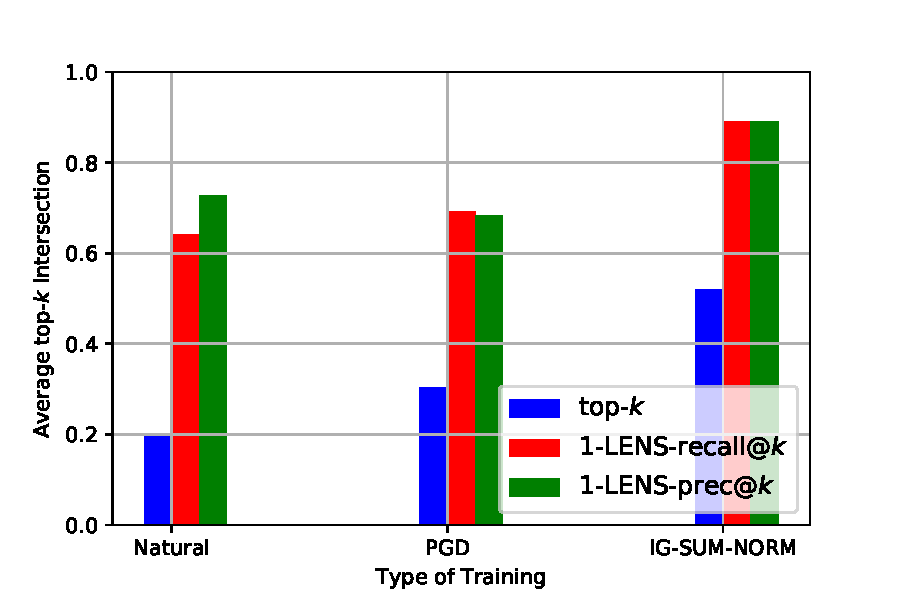
\includegraphics[width=1.0\textwidth]{./plots/mnist_topk_attack_new_metric_sg.pdf}
    \caption{MNIST}
    \label{mnist-rand-fig:a}
    \end{subfigure}
    \begin{subfigure}[b]{0.24\textwidth}
    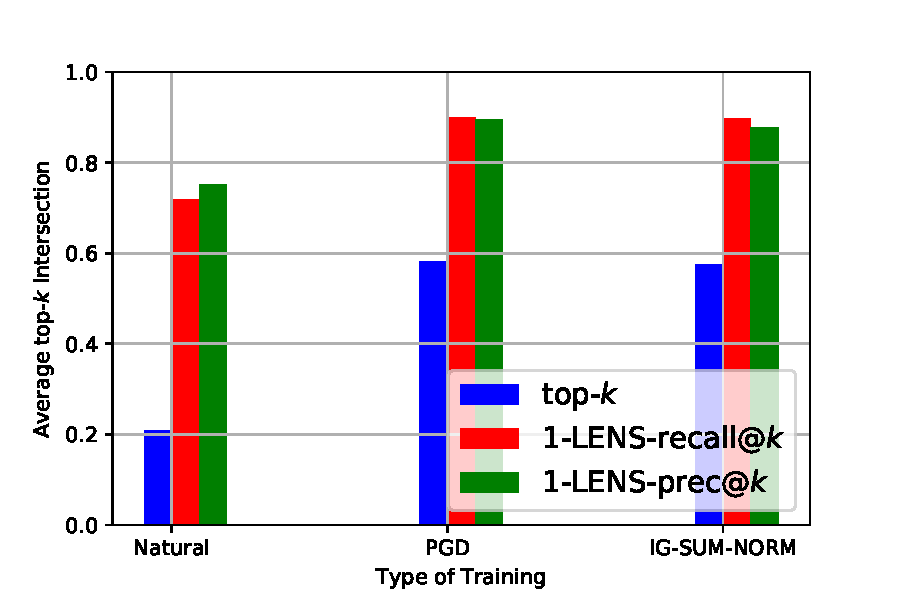
\includegraphics[width=1.0\textwidth]{./plots/fmnist_topk_attack_new_metric_sg.pdf}
    \caption{Fashion MNIST}
    \label{fmnist-rand-fig:b}
    \end{subfigure}\\
    \begin{subfigure}[b]{0.24\textwidth}
    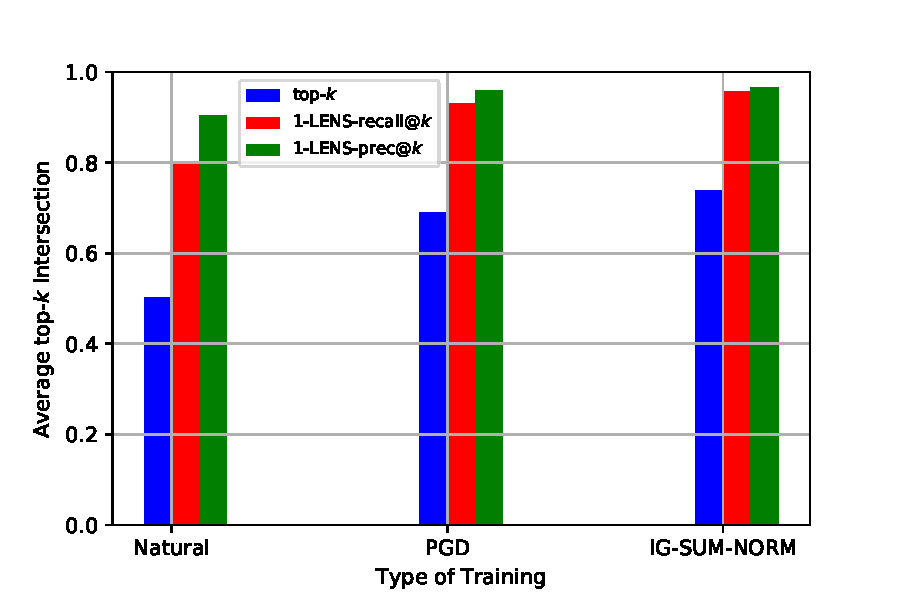
\includegraphics[width=1.0\textwidth]{./plots/gtsrb_topk_attack_new_metric_sg.pdf}
    \caption{GTSRB}
    \label{gtsrb-rand-fig:c}
    \end{subfigure}
    \begin{subfigure}[b]{0.24\textwidth}
    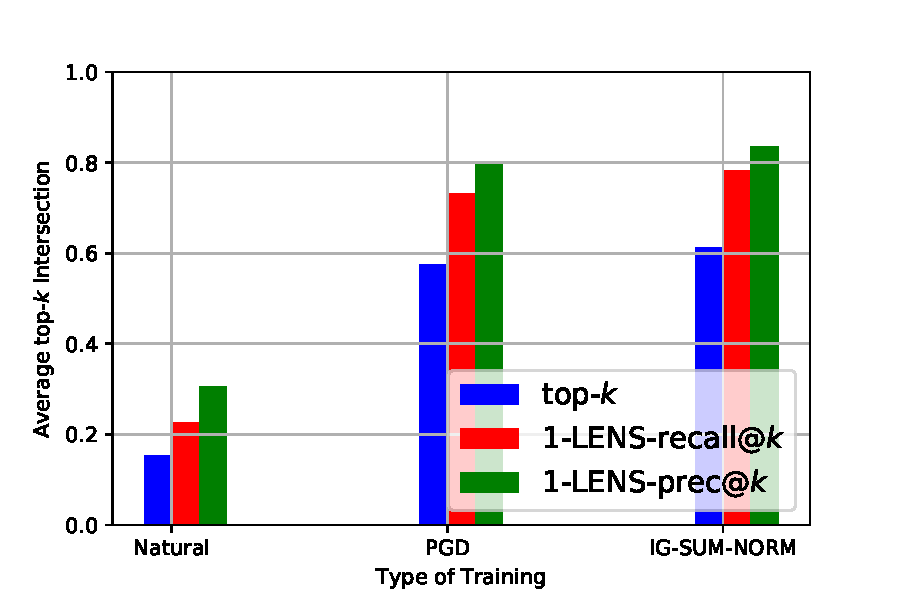
\includegraphics[width=1.0\textwidth]{./plots/flower_topk_3x3_attack_new_metric_sg.pdf}
    \caption{Flower}
    \label{flower-rand-fig:d}
    \end{subfigure}
\end{subfigure}
\caption{Attributional robustness of Simple Gradients on naturally, PGD and IG-SUM-NORM trained models measured as top-$k$ intersection, $1$-LENS-prec@$k$ and $1$-LENS-recall@$k$ between the Simple Gradient of the original images and the Simple Gradient of their perturbations obtained by the {\bf top-$k$} attack \citep{ghorbani2018interpretation} across different datasets.} 
\label{topk-new-metric-training-method-sg}     
\end{figure}


\begin{figure}[!ht]
\centering
\begin{subfigure}[b]{1.0\textwidth}
    \begin{subfigure}[b]{0.24\textwidth}
    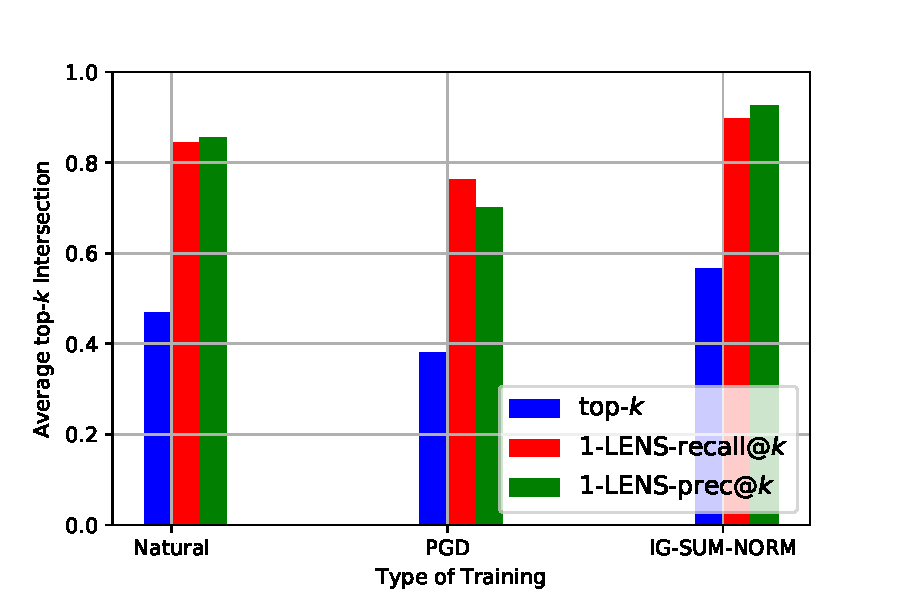
\includegraphics[width=1.0\textwidth]{./plots/mnist_random_attack_new_metric_sg.pdf}
    \caption{MNIST}
    \label{mnist-rand-fig:a}
    \end{subfigure}
    \begin{subfigure}[b]{0.24\textwidth}
    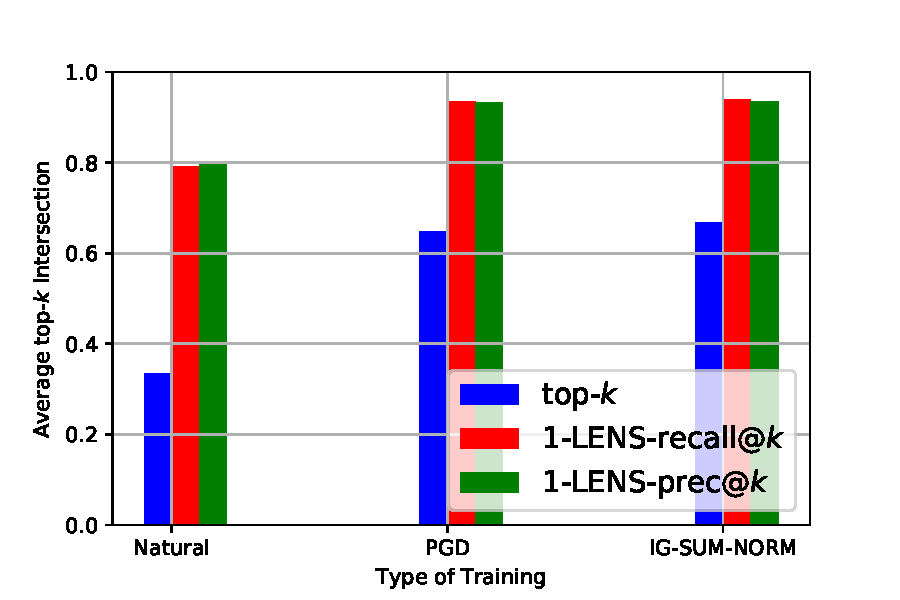
\includegraphics[width=1.0\textwidth]{./plots/fmnist_random_attack_new_metric_sg.pdf}
    \caption{Fashion MNIST}
    \label{fmnist-rand-fig:b}
    \end{subfigure}\\
    \begin{subfigure}[b]{0.24\textwidth}
    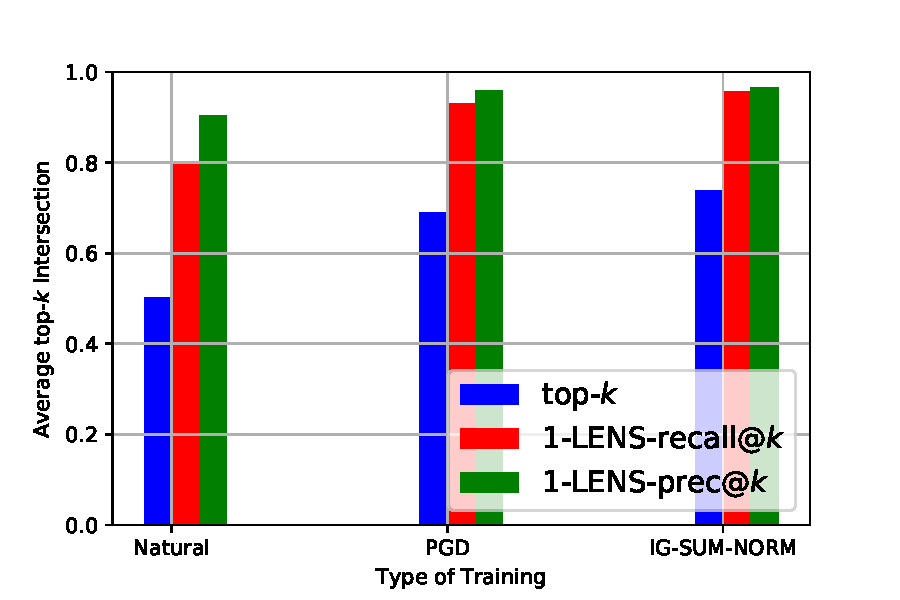
\includegraphics[width=1.0\textwidth]{./plots/gtsrb_random_attack_new_metric_sg.pdf}
    \caption{GTSRB}
    \label{gtsrb-rand-fig:c}
    \end{subfigure}
    \begin{subfigure}[b]{0.24\textwidth}
    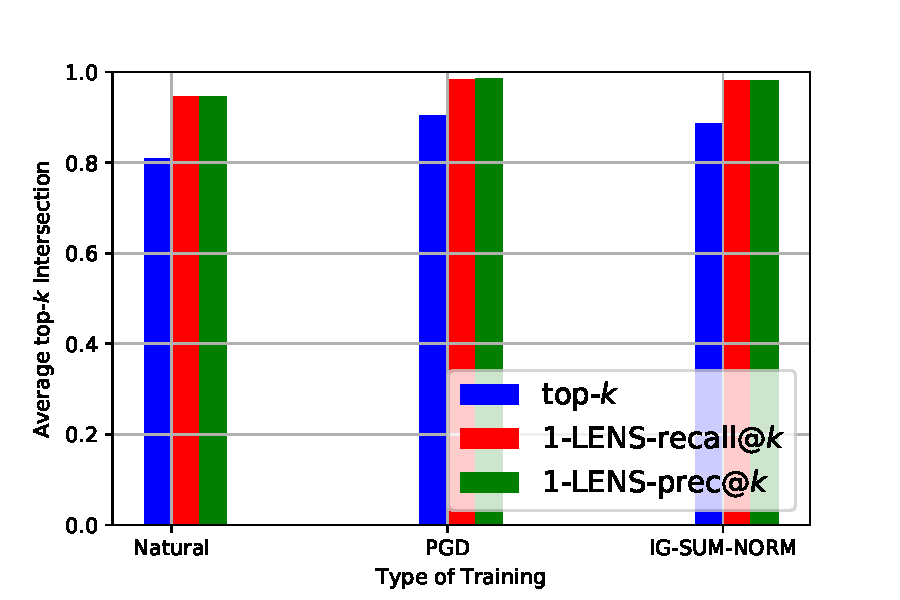
\includegraphics[width=1.0\textwidth]{./plots/flower_random_3x3_attack_new_metric_sg.pdf}
    \caption{Flower}
    \label{flower-rand-fig:d}
    \end{subfigure}
\end{subfigure}
\caption{Attributional robustness of Simple Gradients on naturally, PGD and IG-SUM-NORM trained models measured as top-$k$ intersection, $1$-LENS-prec@$k$ and $1$-LENS-recall@$k$ between the Simple Gradient of the original images and the Simple Gradient of their perturbations obtained by the {\bf random sign} attack \citep{ghorbani2018interpretation} across different datasets.} 
\label{rand-new-metric-training-method-sg}     
\end{figure}

\begin{figure}[!ht]
\centering
\begin{subfigure}[b]{1.0\textwidth}
    \begin{subfigure}[b]{0.24\textwidth}
    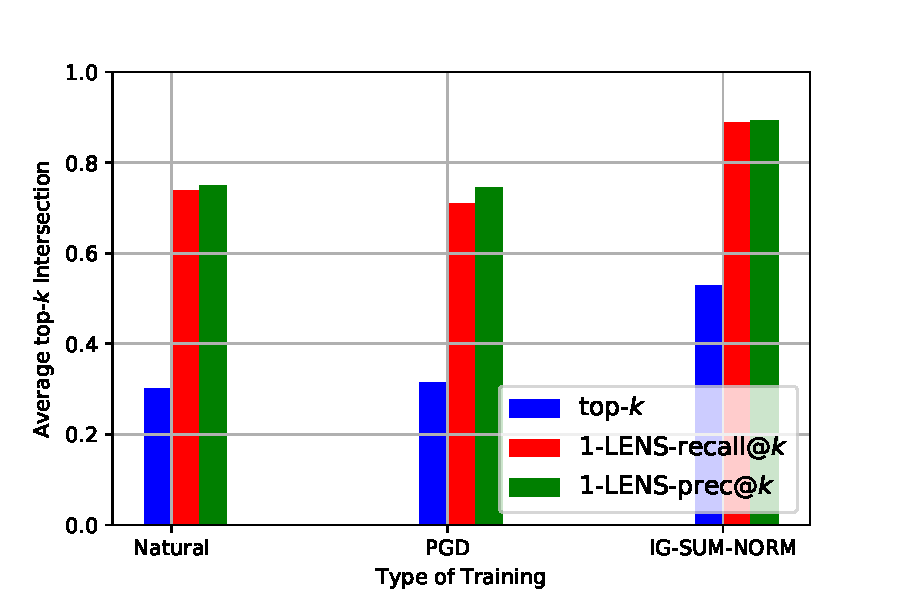
\includegraphics[width=1.0\textwidth]{./plots/mnist_mc_attack_new_metric_sg.pdf}
    \caption{MNIST}
    \label{mnist-rand-fig:a}
    \end{subfigure}
    \begin{subfigure}[b]{0.24\textwidth}
    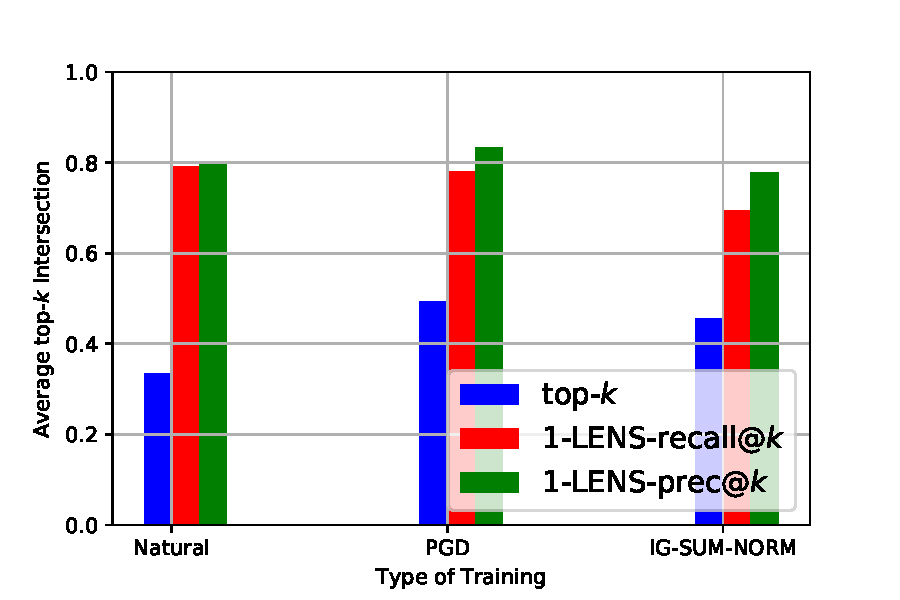
\includegraphics[width=1.0\textwidth]{./plots/fmnist_mc_attack_new_metric_sg.pdf}
    \caption{Fashion MNIST}
    \label{fmnist-rand-fig:b}
    \end{subfigure}\\
    %\begin{subfigure}[b]{0.24\textwidth}
    %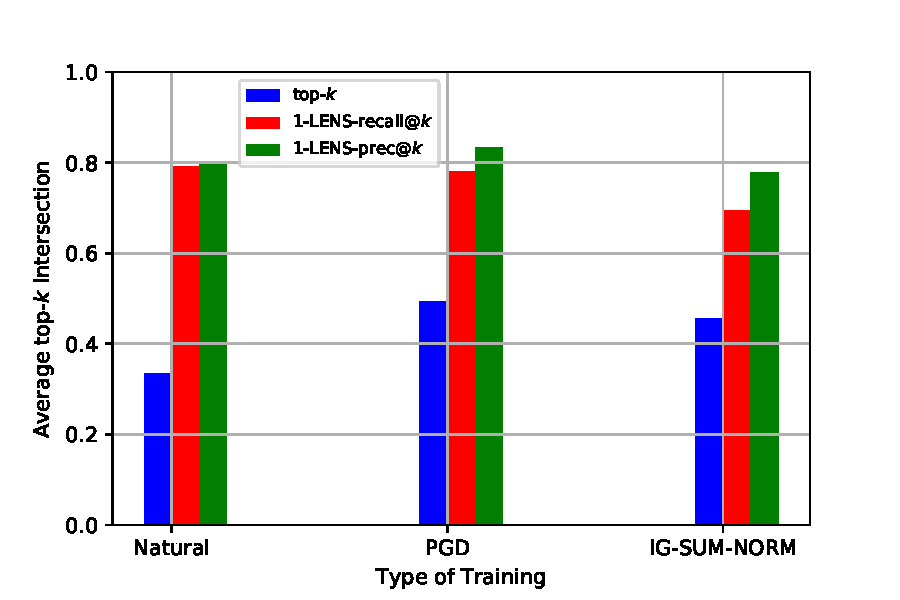
\includegraphics[width=1.0\textwidth]{./plots/gtsrb_mc_attack_new_metric_sg.pdf}
    %\caption{GTSRB}
    %\label{gtsrb-rand-fig:c}
    %\end{subfigure}
    \begin{subfigure}[b]{0.24\textwidth}
    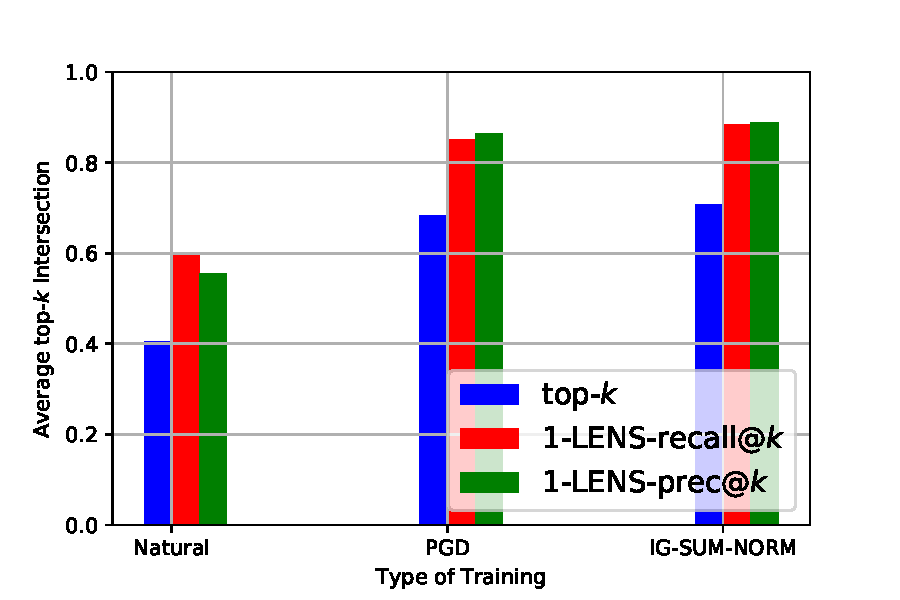
\includegraphics[width=1.0\textwidth]{./plots/flower_mc_3x3_attack_new_metric_sg.pdf}
    \caption{Flower}
    \label{flower-rand-fig:d}
    \end{subfigure}
\end{subfigure}
\caption{Attributional robustness of Simple Gradients on naturally, PGD and IG-SUM-NORM trained models measured as top-$k$ intersection, $1$-LENS-prec@$k$ and $1$-LENS-recall@$k$ between the Simple Gradient of the original images and the Simple Gradient of their perturbations obtained by the {\bf mass center} attack \citep{ghorbani2018interpretation} across different datasets.} 
\label{mc-new-metric-training-method-sg}     
\end{figure}

\begin{figure}[!ht]
\centering
\begin{subfigure}[b]{1.0\textwidth}
    \begin{subfigure}[b]{0.24\textwidth}
    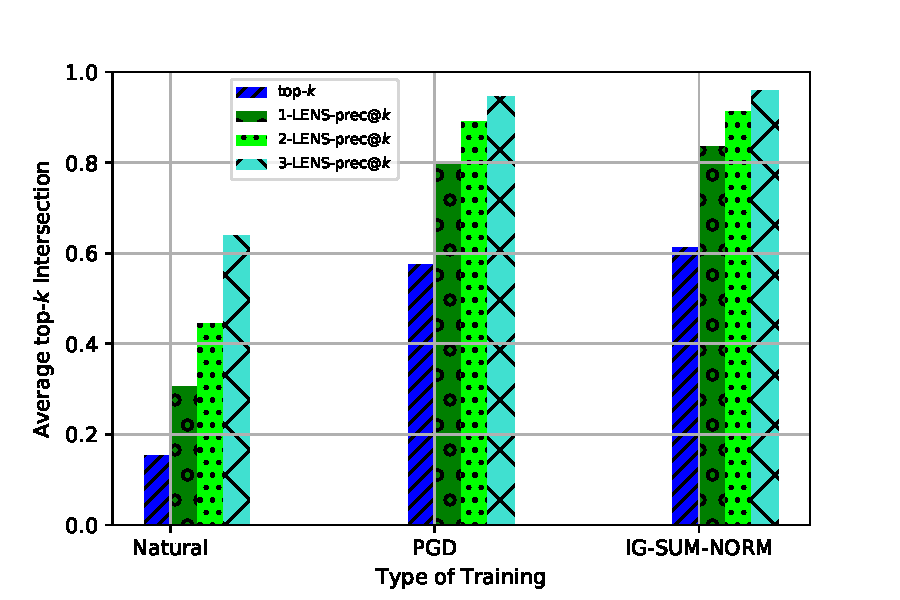
\includegraphics[width=1.0\textwidth]{./plots/flower_topk_attack_new_metric_sg.pdf}
    \caption{SG : top-$k$}
    \label{mnist-rand-fig:a}
    \end{subfigure}
    \begin{subfigure}[b]{0.24\textwidth}
    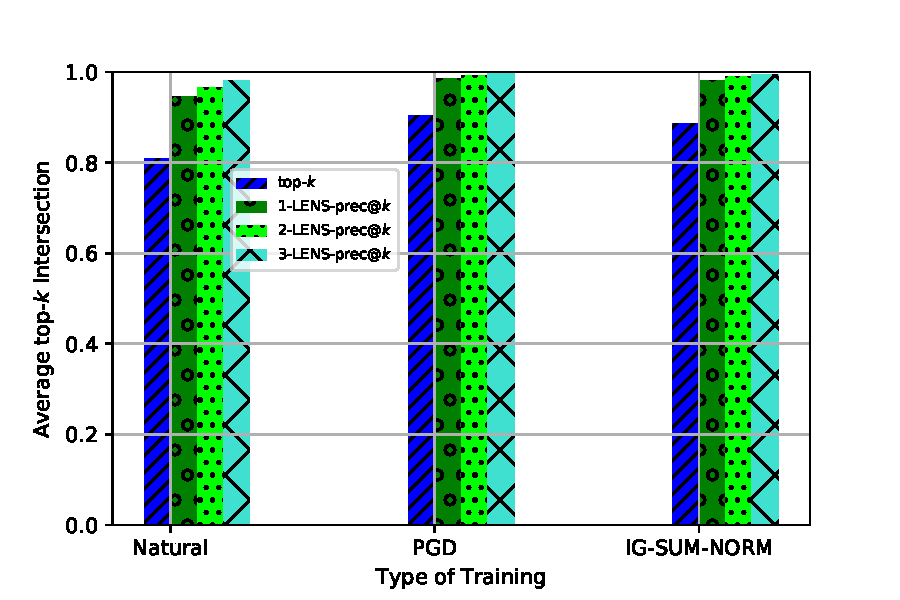
\includegraphics[width=1.0\textwidth]{./plots/flower_random_attack_new_metric_sg.pdf}
    \caption{SG : random}
    \label{mnist-rand-fig:b}
    \end{subfigure}\\
    \begin{subfigure}[b]{0.24\textwidth}
    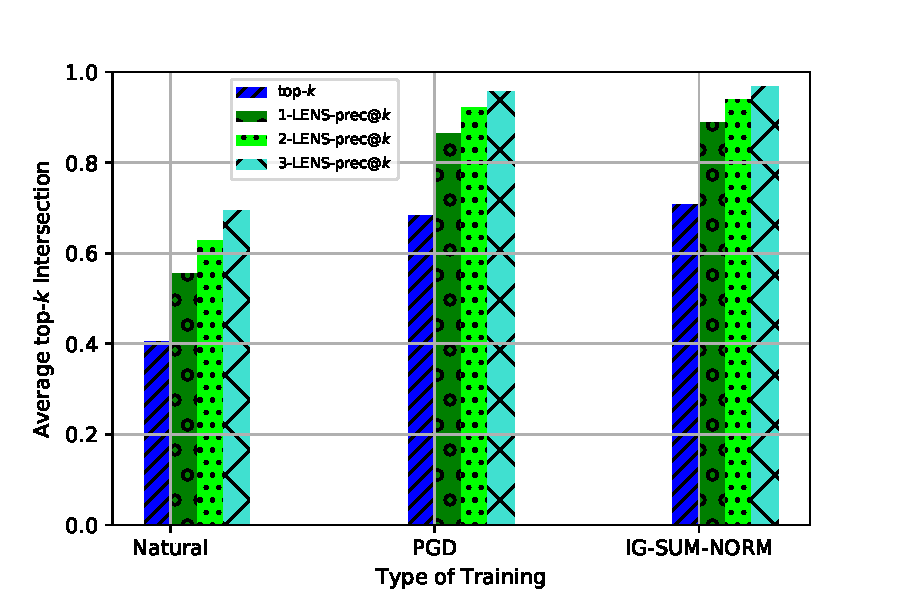
\includegraphics[width=1.0\textwidth]{./plots/flower_mc_attack_new_metric_sg.pdf}
    \caption{SG : center of mass}
    \label{mnist-rand-fig:c}
    \end{subfigure}
\end{subfigure}
\caption{Attributional robustness of Simple Gradients on naturally, PGD and IG-SUM-NORM trained models measured as top-$k$ intersection and $w$-LENS-prec@$k$ between the IG of the original images and the IG of their perturbations. Perturbations are obtained by the top-$k$ attack and the mass center attack \citep{ghorbani2018interpretation} as well as a random perturbation. The plots show the effect of varying $w$ on Flower dataset.}
\label{flower-topk-new-metric-training-method-sg}     
\end{figure}

\clearpage

\subsection{Experiments with Other Explanation Methods} \label{app:all-other-exp}

In this section we present all the results with other explanation methods other than IG and SG shown in previous sections with naturally and PGD trained models using mainly random sign perturbation.

\begin{comment}
 \begin{figure}[h]
 \centering
     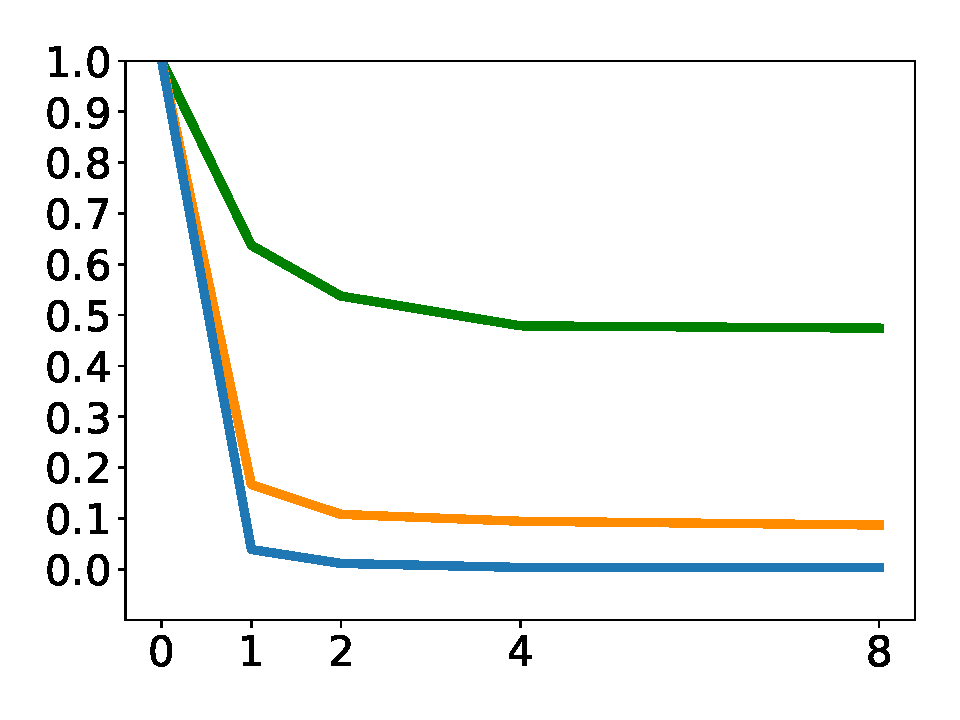
\includegraphics[width=0.38\textwidth]{./plots/imagenet_gh_lens_dl_orig_pert_all.pdf}    
    \caption{Similar to Figure \ref{imagenet-ghorbani-with-lens-div}, we plot average top-$k$ intersection (currently used metric), $3$-LENS-recall@$k$ and $3$-LENS-recall@$k$-div (proposed metrics) against the $\ell_{\infty}$-norm of  attributional attack perturbations for {\bf DeepLIFT} \citep{shrikumar2019learning} of a SqueezeNet model on ImageNet. We only present results with {\bf $\epsilon=8/255$} here, while in Figure \ref{imagenet-ghorbani-with-lens-div} $\epsilon=\{1/255, 2/255, 4/255, 8/255\}$ were plotted. We use $k=1000$ and three attributional attack variants proposed by \citet{ghorbani2018interpretation}. Evidently, the proposed metrics show more robustness under the same attacks.}
\label{imagenet-ghorbani-with-lens-div-dl}     
\end{figure}
\end{comment}

\begin{figure*}[t]
 \centering
 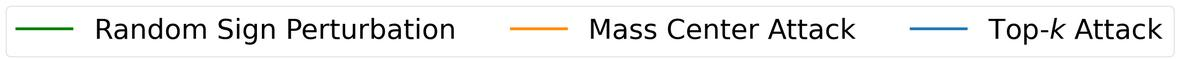
\includegraphics[width=0.80\textwidth]{./images/fig-2-legend-plots.jpg}\\
     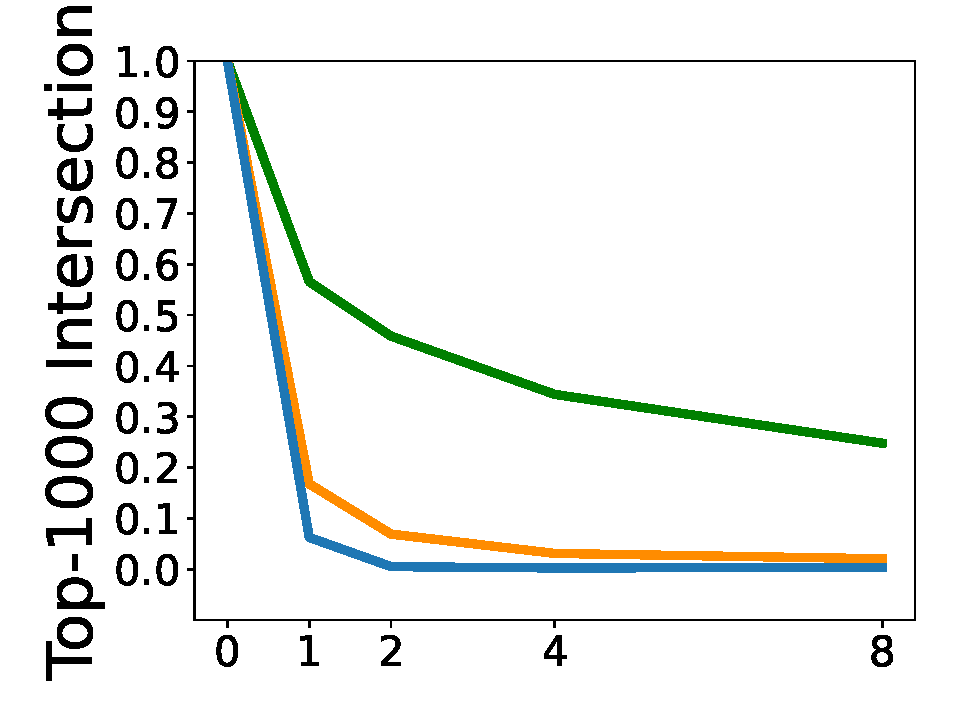
\includegraphics[width=0.23\textwidth]{./plots/imagenet_gh_lens_sg_orig_pert_all.pdf}
     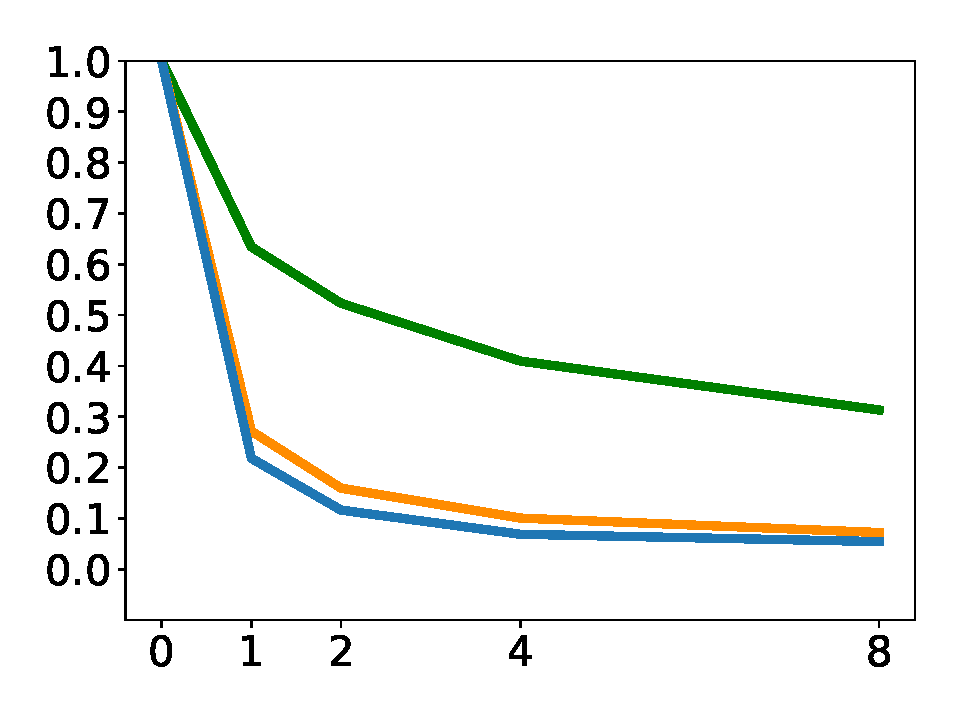
\includegraphics[width=0.23\textwidth]{./plots/imagenet_gh_lens_ig_orig_pert_all.pdf}
     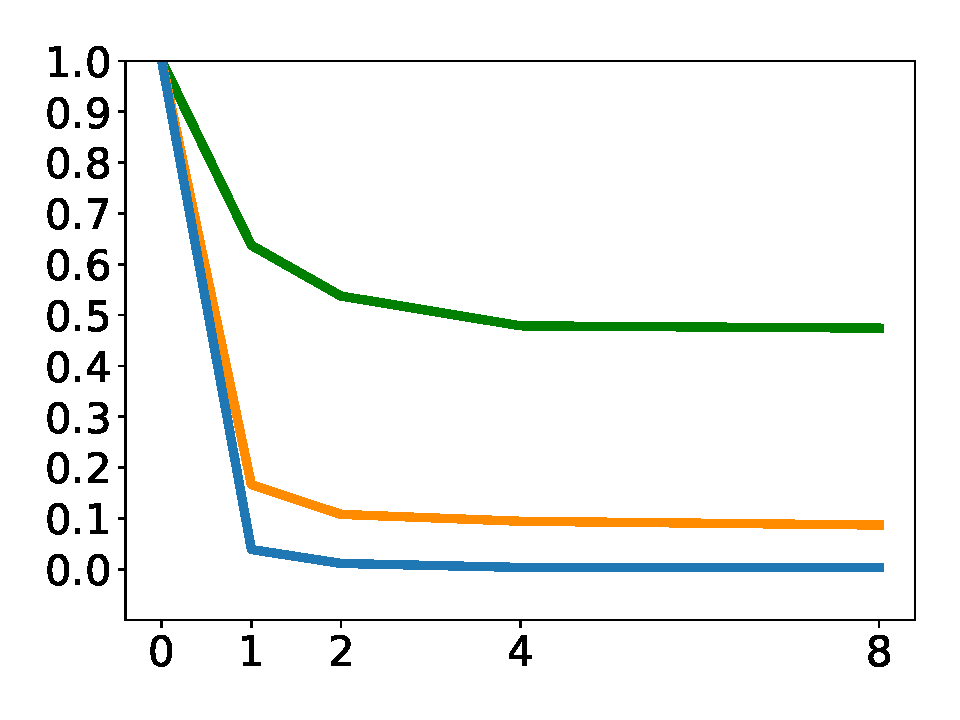
\includegraphics[width=0.23\textwidth]{./plots/imagenet_gh_lens_dl_orig_pert_all.pdf}
     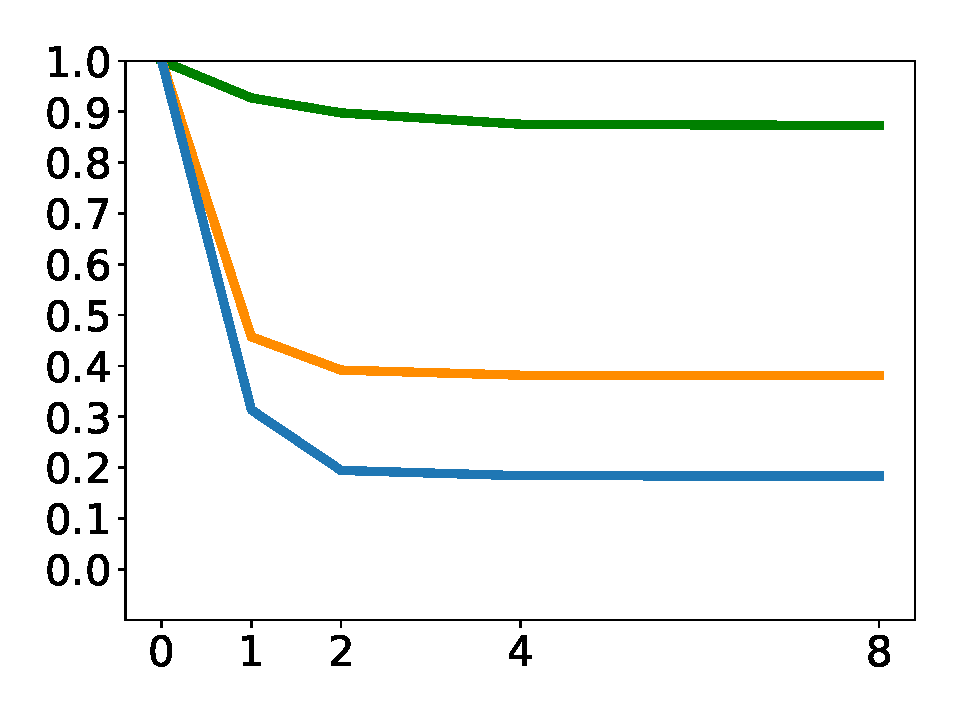
\includegraphics[width=0.23\textwidth]{./plots/imagenet_gh_lens_dtd_orig_pert_all.pdf}\\
     
     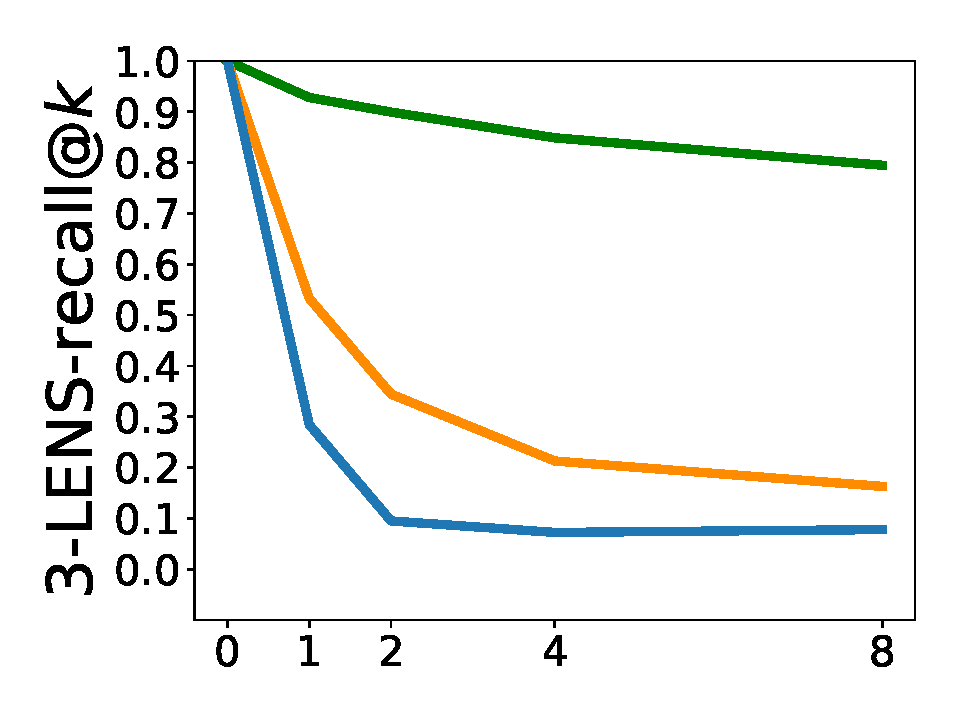
\includegraphics[width=0.23\textwidth]{./plots/imagenet_gh_lens_sg_orig_pert_all_lens.pdf}
     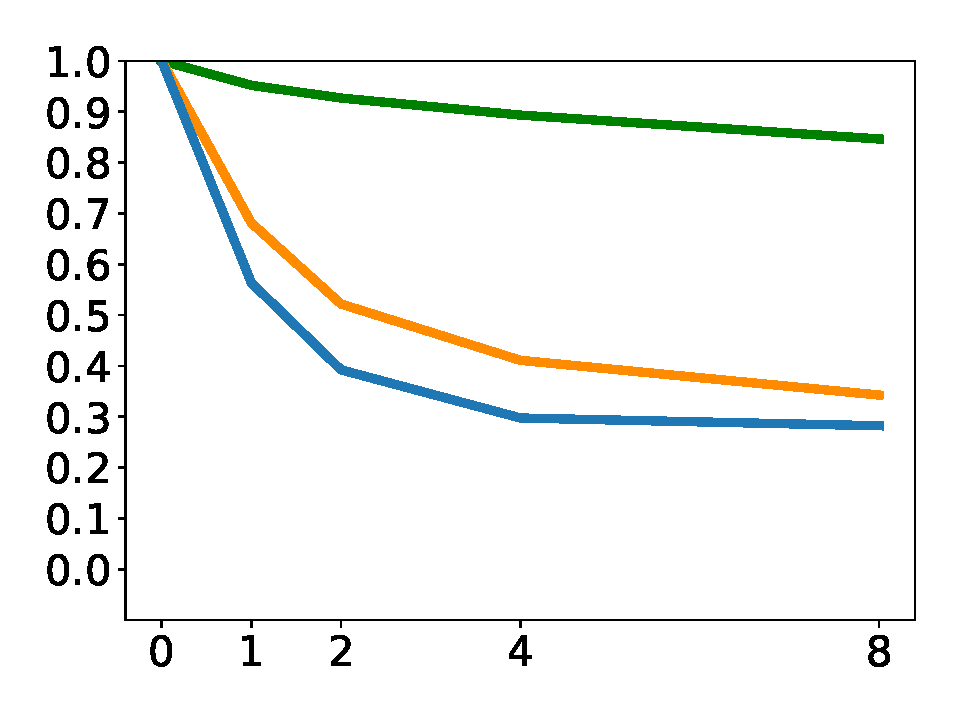
\includegraphics[width=0.23\textwidth]{./plots/imagenet_gh_lens_ig_orig_pert_all_lens.pdf}         
     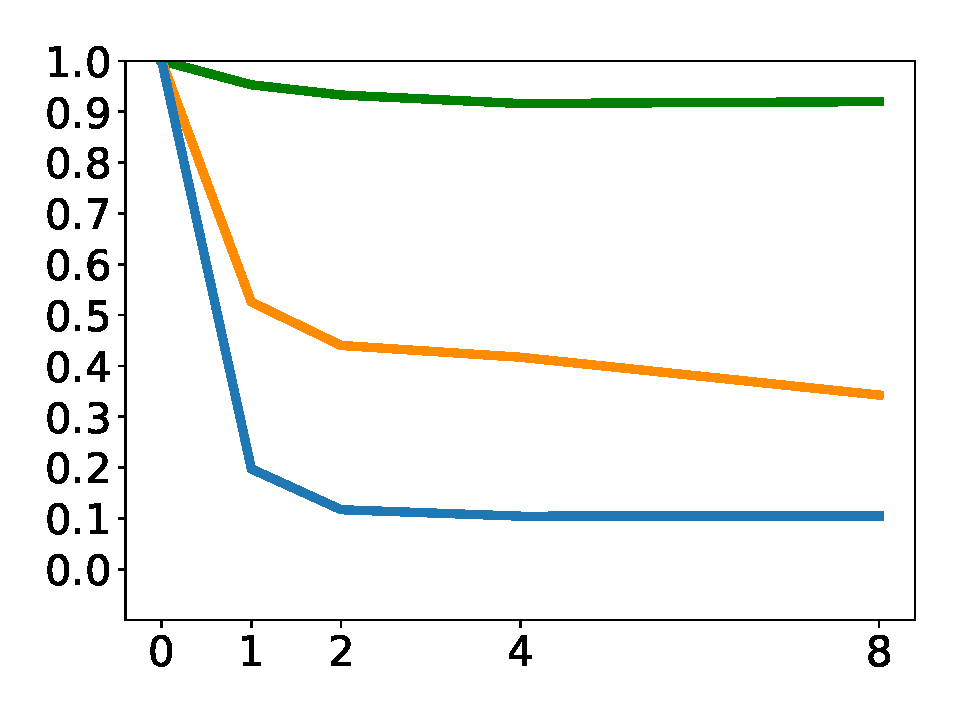
\includegraphics[width=0.23\textwidth]{./plots/imagenet_gh_lens_dl_orig_pert_all_lens.pdf}
     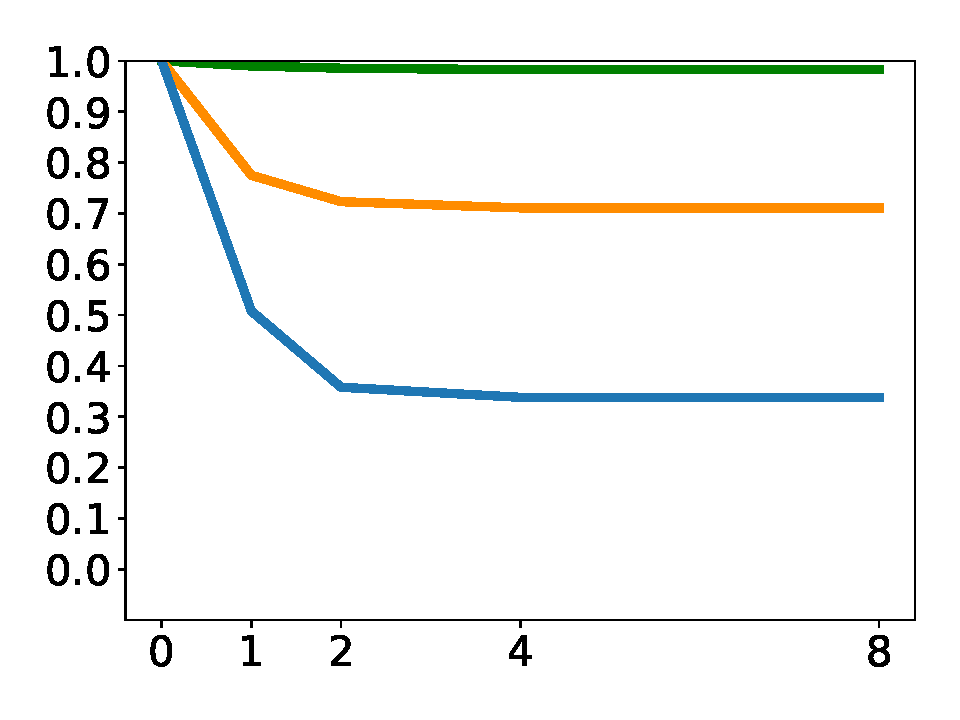
\includegraphics[width=0.23\textwidth]{./plots/imagenet_gh_lens_dtd_orig_pert_all_lens.pdf}\\     
     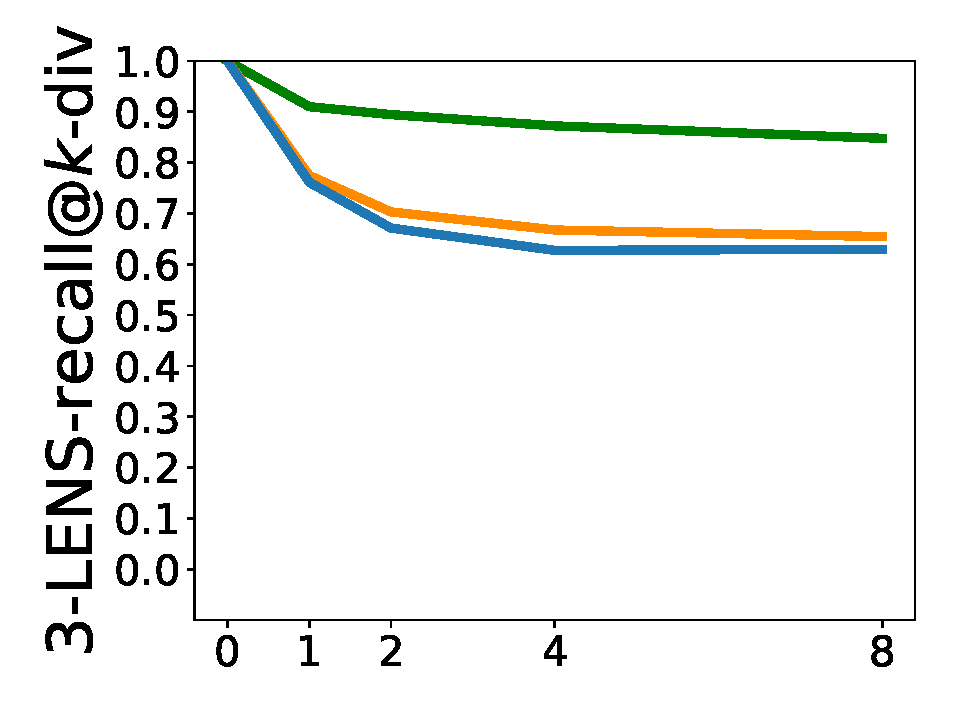
\includegraphics[width=0.23\textwidth]{./plots/imagenet_gh_lens_sg_orig_pert_all_div.pdf}     
     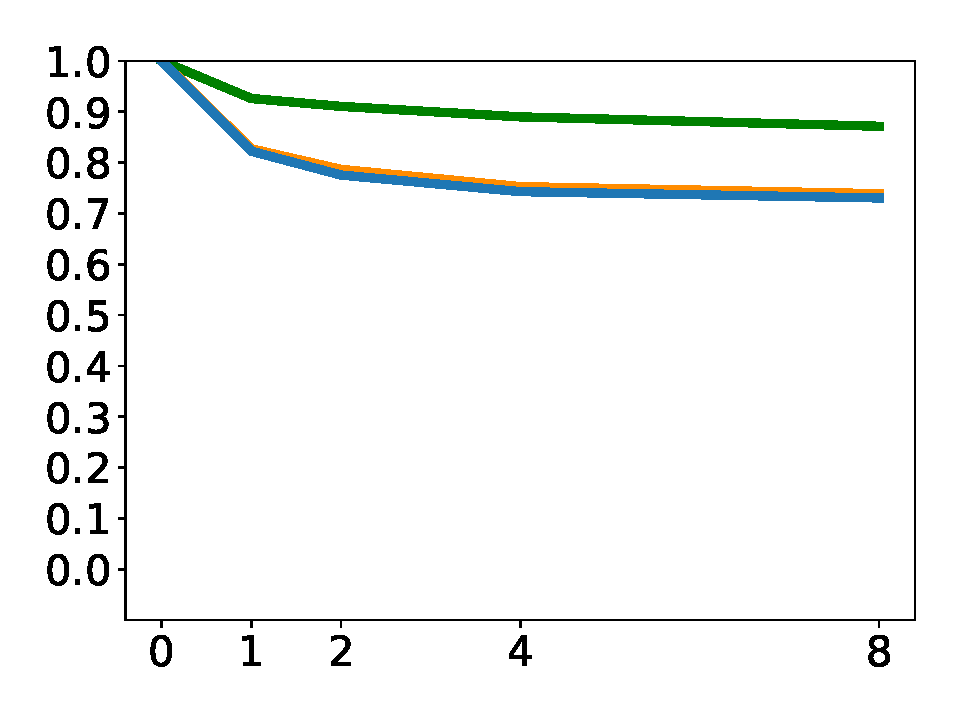
\includegraphics[width=0.23\textwidth]{./plots/imagenet_gh_lens_ig_orig_pert_all_div.pdf}     
     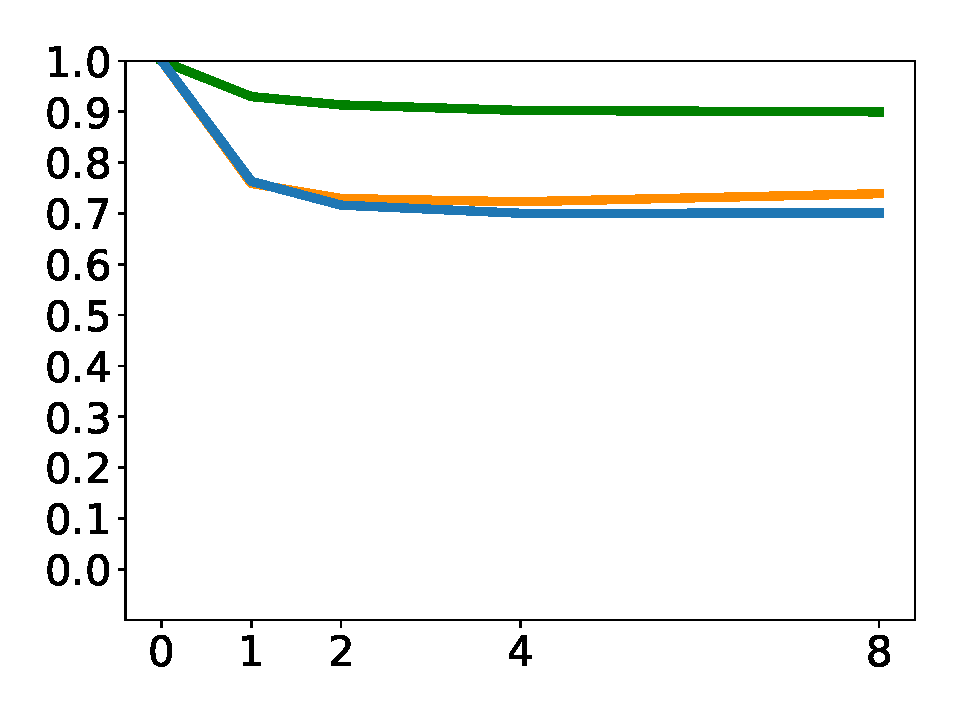
\includegraphics[width=0.23\textwidth]{./plots/imagenet_gh_lens_dl_orig_pert_all_div.pdf}    
     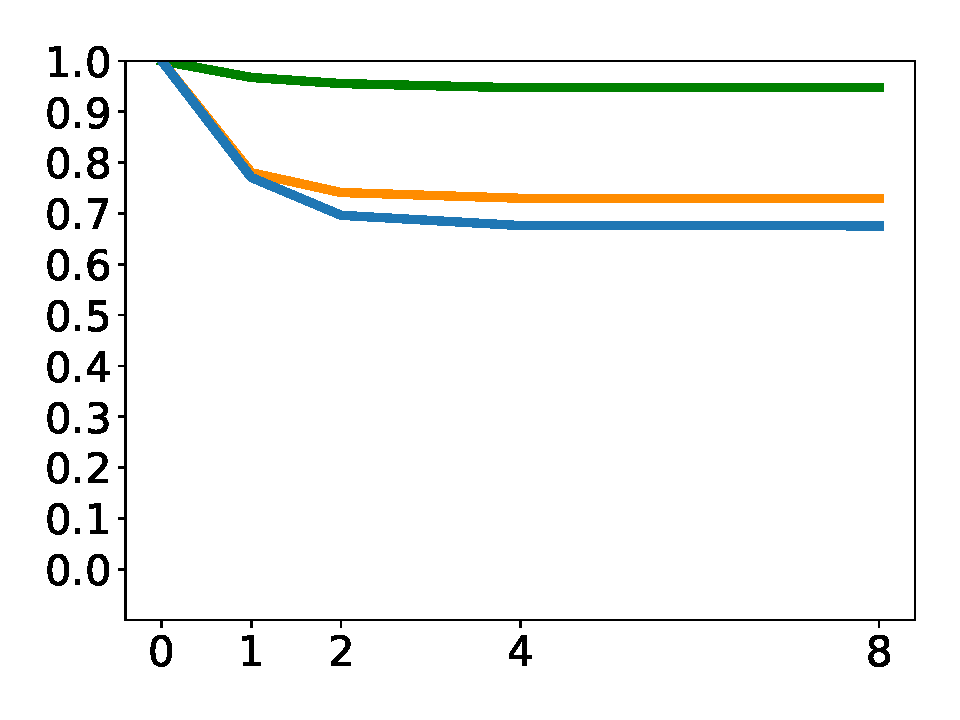
\includegraphics[width=0.23\textwidth]{./plots/imagenet_gh_lens_dtd_orig_pert_all_div.pdf}\\
     
\includegraphics[width=0.20\textwidth]{./images/fig-2-x-axis.jpg}
    \caption{\footnotesize Similar to Figure \ref{imagenet-ghorbani-with-lens-div}, From top to bottom, we plot average top-$k$ intersection (currently used metric, \textbf{\textit{top}}), $3$-LENS-recall@$k$ and $3$-LENS-recall@$k$-div (proposed metrics, \textbf{\textit{middle}} and \textbf{\textit{bottom}} respectively) against attributional attack perturbations for four attribution methods of a SqueezeNet model (as used by \citet{ghorbani2018interpretation}) on Imagenet: \textit{(left)} Simple Gradients (SG), \textit{(center left)} Integrated Gradients (IG), \textit{(center right)} DeepLift, \textit{(right)} Deep Taylor Decomposition. We use $k=1000$ with an $\ell_{\infty}$-norm attack and three attack variants proposed by \citet{ghorbani2018interpretation}. Evidently, the proposed metrics show more robustness under the same attacks.}
    \vspace{-8pt}
\label{imagenet-ghorbani-with-lens-div-with-dl}     
\end{figure*}

\begin{figure}[!ht]
\centering
\begin{subfigure}[b]{1.0\textwidth}
    \begin{subfigure}[b]{0.15\textwidth}
    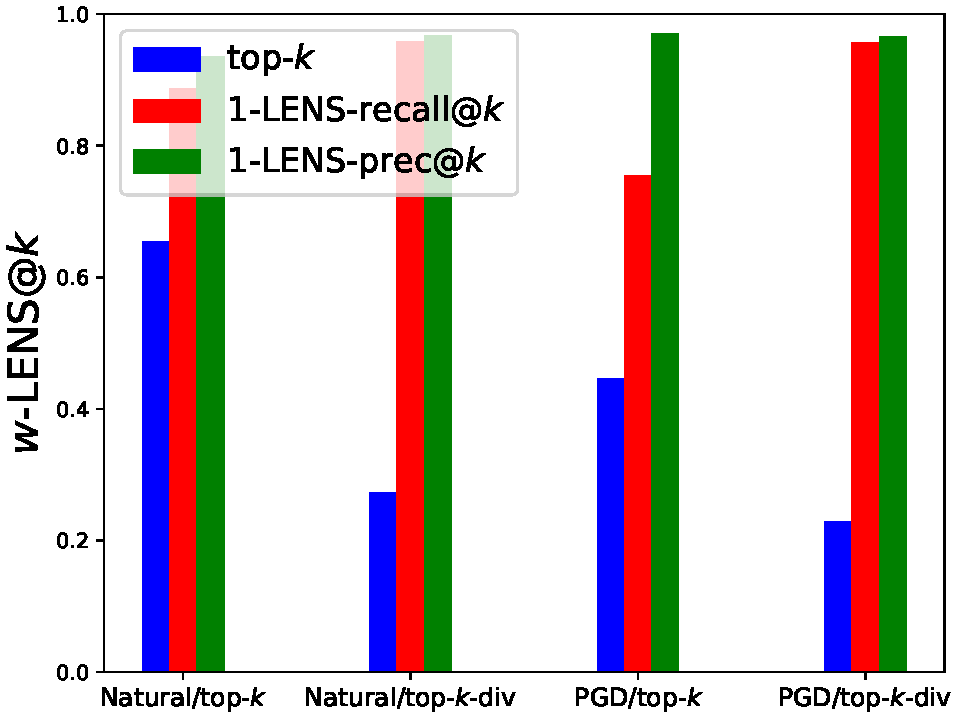
\includegraphics[width=1.0\textwidth]{./plots/mnist_nat_pgd_rand_sg_lens_div_both_lens.pdf}
    \caption{MNIST}
    \label{mnist-rand-fig:a}
    \end{subfigure}
    \begin{subfigure}[b]{0.15\textwidth}
    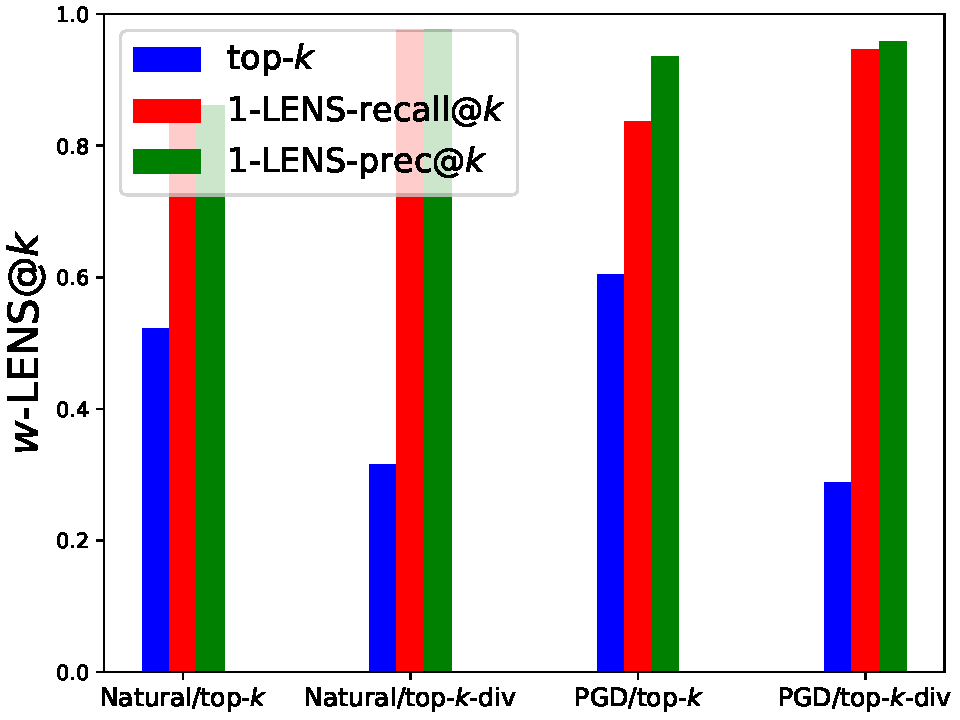
\includegraphics[width=1.0\textwidth]{./plots/fmnist_nat_pgd_rand_sg_lens_div_both_lens.pdf}
    \caption{Fashion MNIST}
    \label{fmnist-rand-fig:b}
    \end{subfigure}
    \begin{subfigure}[b]{0.15\textwidth}
    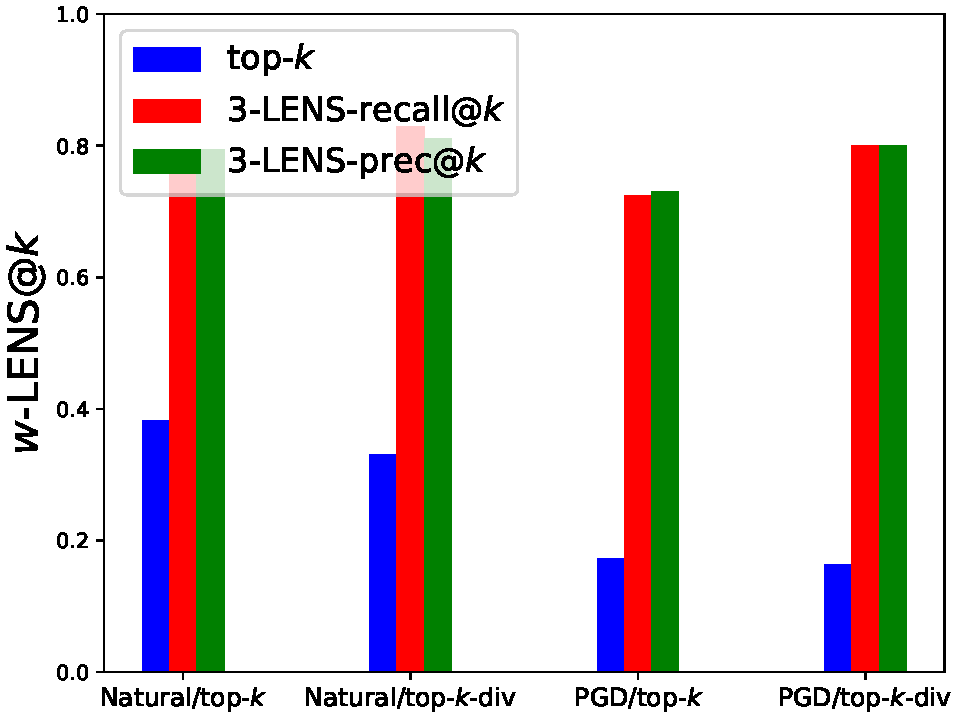
\includegraphics[width=1.0\textwidth]{./plots/imagenet_nat_pgd_rand_sg_lens_div_both_lens.pdf}
    \caption{ImageNet}
    \label{flower-rand-fig:d}
    \end{subfigure}
\end{subfigure}
\caption{Attributional robustness of Simple Gradients(SG) on naturally and PGD trained models measured as top-$k$ intersection, $w$-LENS-prec@$k$ and $w$-LENS-recall@$k$ between the {\bf Simple Gradients(SG)} of the original images and of their perturbations obtained by the random sign perturbation across different datasets.} 
\label{all-datasets-topk-div-both-lens-sg}
\end{figure}

\begin{figure}[!ht]
\centering
\begin{subfigure}[b]{1.0\textwidth}
    \begin{subfigure}[b]{0.15\textwidth}
    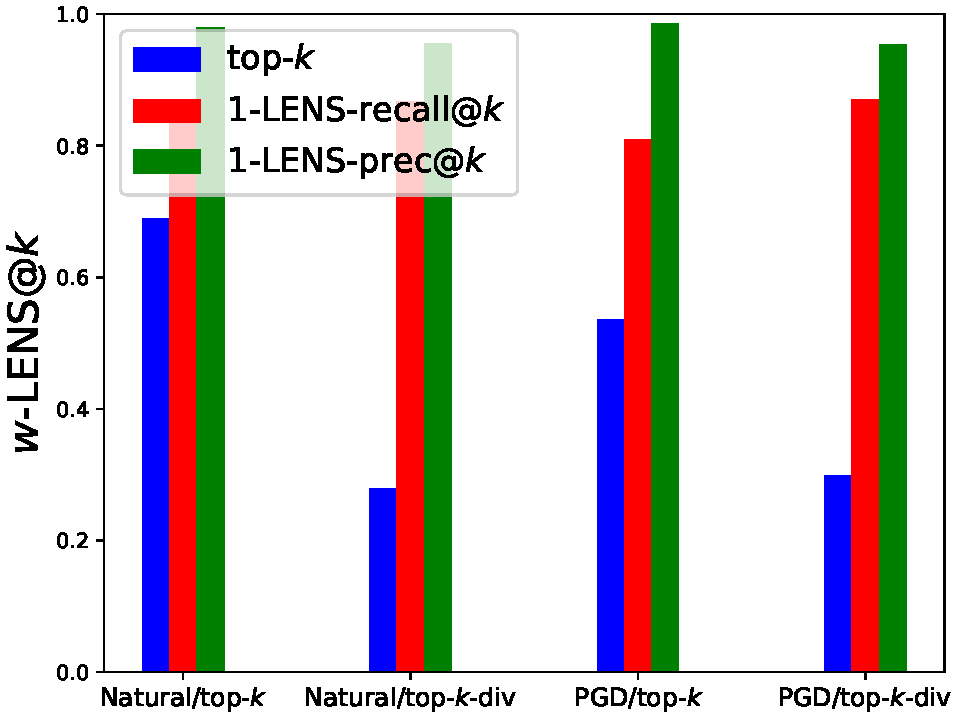
\includegraphics[width=1.0\textwidth]{./plots/mnist_nat_pgd_rand_ixg_lens_div_both_lens.pdf}
    \caption{MNIST}
    \label{mnist-rand-fig:a}
    \end{subfigure}
    \begin{subfigure}[b]{0.15\textwidth}
    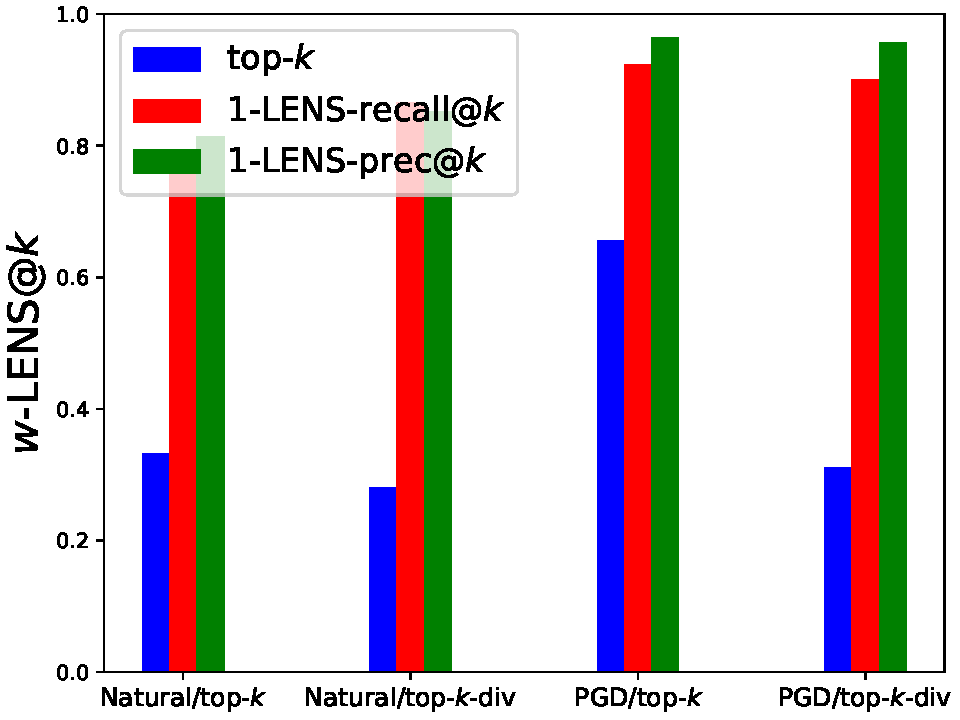
\includegraphics[width=1.0\textwidth]{./plots/fmnist_nat_pgd_rand_ixg_lens_div_both_lens.pdf}
    \caption{Fashion MNIST}
    \label{fmnist-rand-fig:b}
    \end{subfigure}
    \begin{subfigure}[b]{0.15\textwidth}
    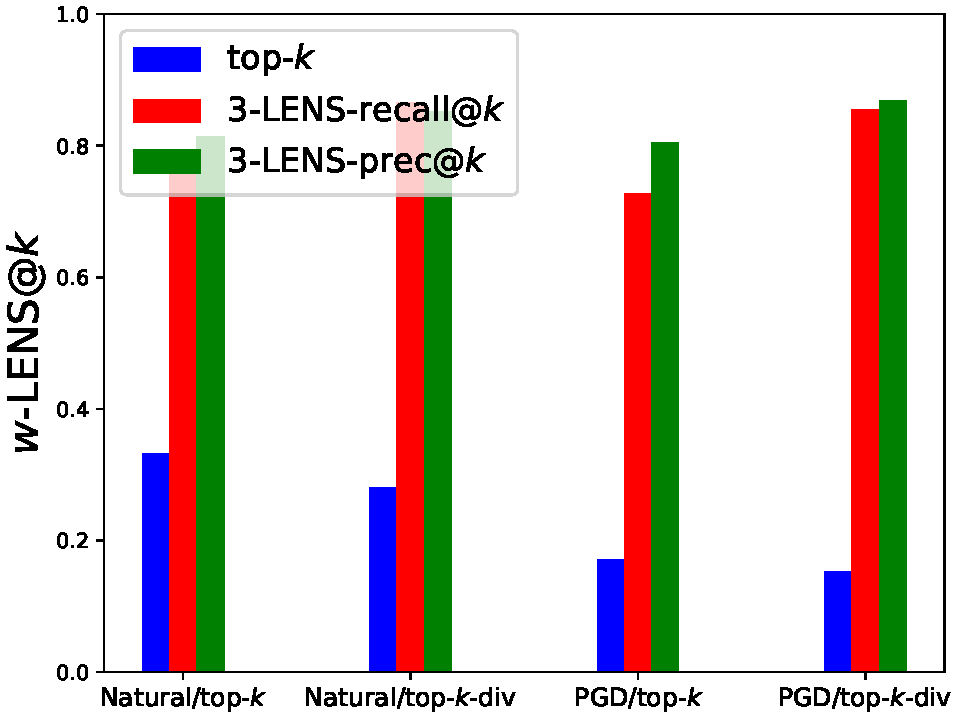
\includegraphics[width=1.0\textwidth]{./plots/imagenet_nat_pgd_rand_ixg_lens_div_both_lens.pdf}
    \caption{ImageNet}
    \label{flower-rand-fig:d}
    \end{subfigure}
\end{subfigure}
\caption{Attributional robustness of Image $\times$ Gradients on naturally and PGD trained models measured as top-$k$ intersection, $w$-LENS-prec@$k$ and $w$-LENS-recall@$k$ between the {\bf Image $\times$ Gradients} of the original images and of their perturbations obtained by the random sign perturbation across different datasets.} 
\label{all-datasets-topk-div-both-lens-ixg}
\end{figure}

\begin{figure}[!ht]
\centering
\begin{subfigure}[b]{1.0\textwidth}
    \begin{subfigure}[b]{0.15\textwidth}
    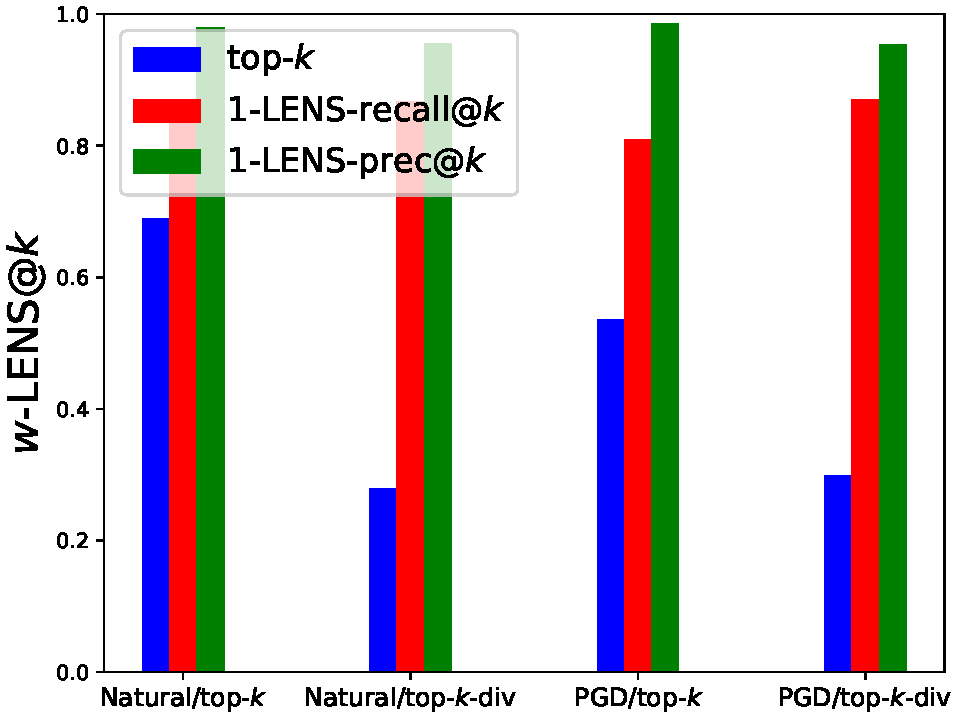
\includegraphics[width=1.0\textwidth]{./plots/mnist_nat_pgd_rand_lrp_lens_div_both_lens.pdf}
    \caption{MNIST}
    \label{mnist-rand-fig:a}
    \end{subfigure}
    \begin{subfigure}[b]{0.15\textwidth}
    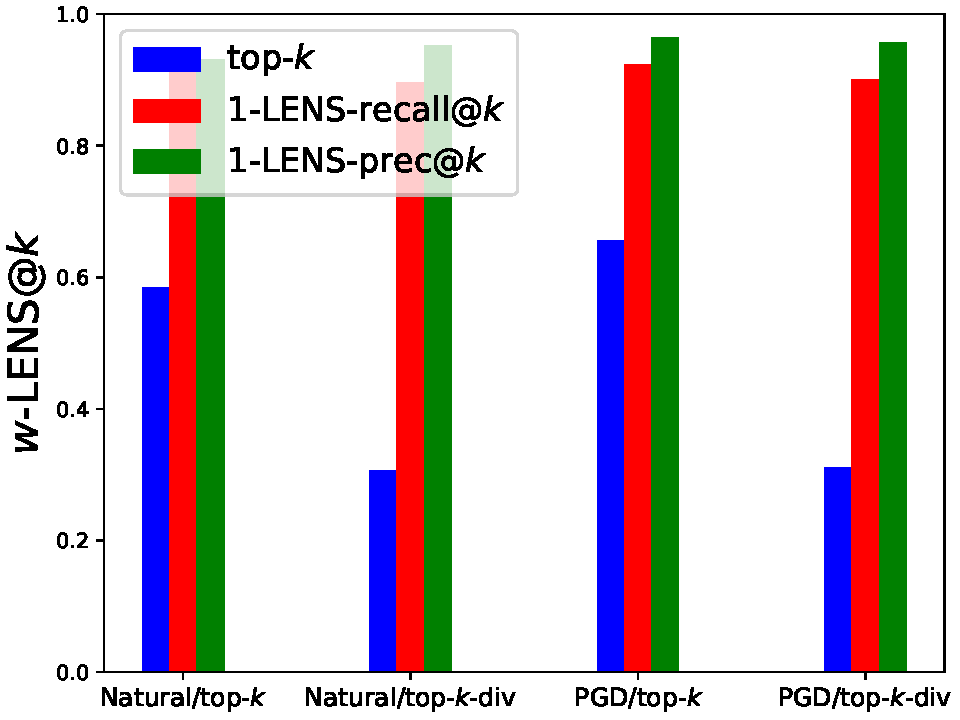
\includegraphics[width=1.0\textwidth]{./plots/fmnist_nat_pgd_rand_lrp_lens_div_both_lens.pdf}
    \caption{Fashion MNIST}
    \label{fmnist-rand-fig:b}
    \end{subfigure}
    \begin{subfigure}[b]{0.15\textwidth}
    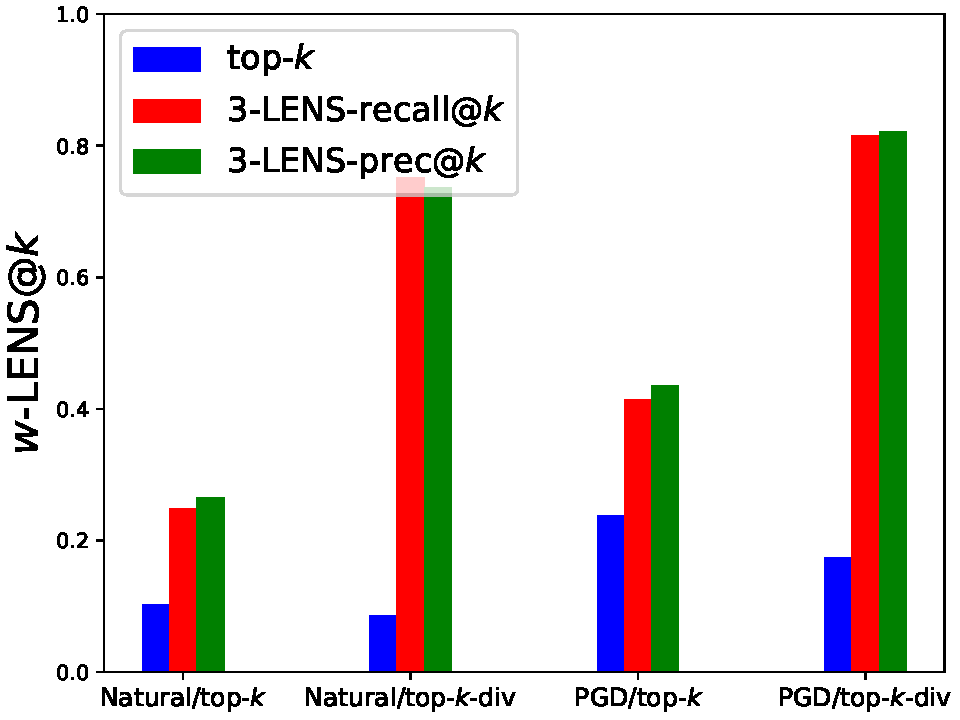
\includegraphics[width=1.0\textwidth]{./plots/imagenet_nat_pgd_rand_lrp_lens_div_both_lens.pdf}
    \caption{ImageNet}
    \label{flower-rand-fig:d}
    \end{subfigure}
\end{subfigure}
\caption{Attributional robustness of LRP \citep{bach2015lrp} on naturally and PGD trained models measured as top-$k$ intersection, $w$-LENS-prec@$k$ and $w$-LENS-recall@$k$ between the {\bf LRP} of the original images and of their perturbations obtained by the random sign perturbation across different datasets.} 
\label{all-datasets-topk-div-both-lens-lrp}
\end{figure}

\begin{figure}[!ht]
\centering
\begin{subfigure}[b]{1.0\textwidth}
    \begin{subfigure}[b]{0.15\textwidth}
    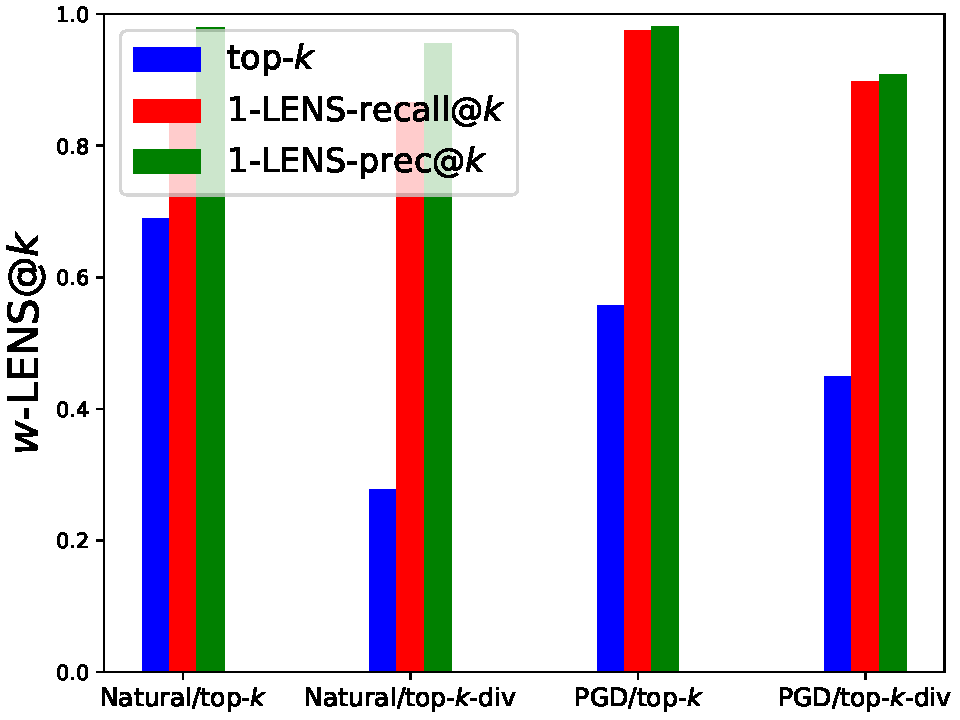
\includegraphics[width=1.0\textwidth]{./plots/mnist_nat_pgd_rand_dl_lens_div_both_lens.pdf}
    \caption{MNIST}
    \label{mnist-rand-fig:a}
    \end{subfigure}
    \begin{subfigure}[b]{0.15\textwidth}
    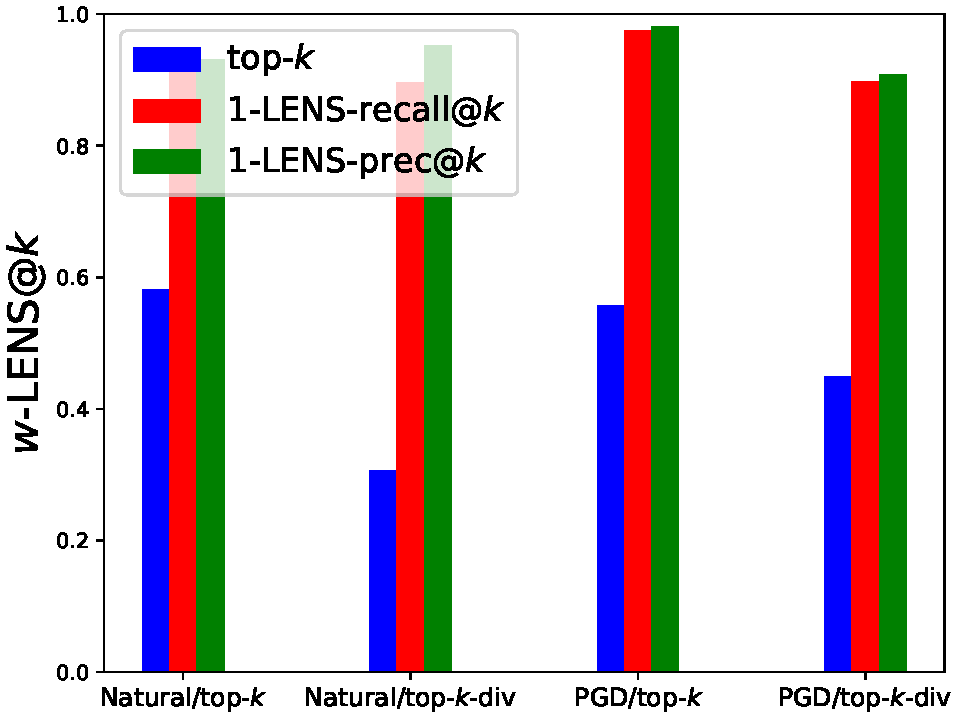
\includegraphics[width=1.0\textwidth]{./plots/fmnist_nat_pgd_rand_dl_lens_div_both_lens.pdf}
    \caption{Fashion MNIST}
    \label{fmnist-rand-fig:b}
    \end{subfigure}
    \begin{subfigure}[b]{0.15\textwidth}
    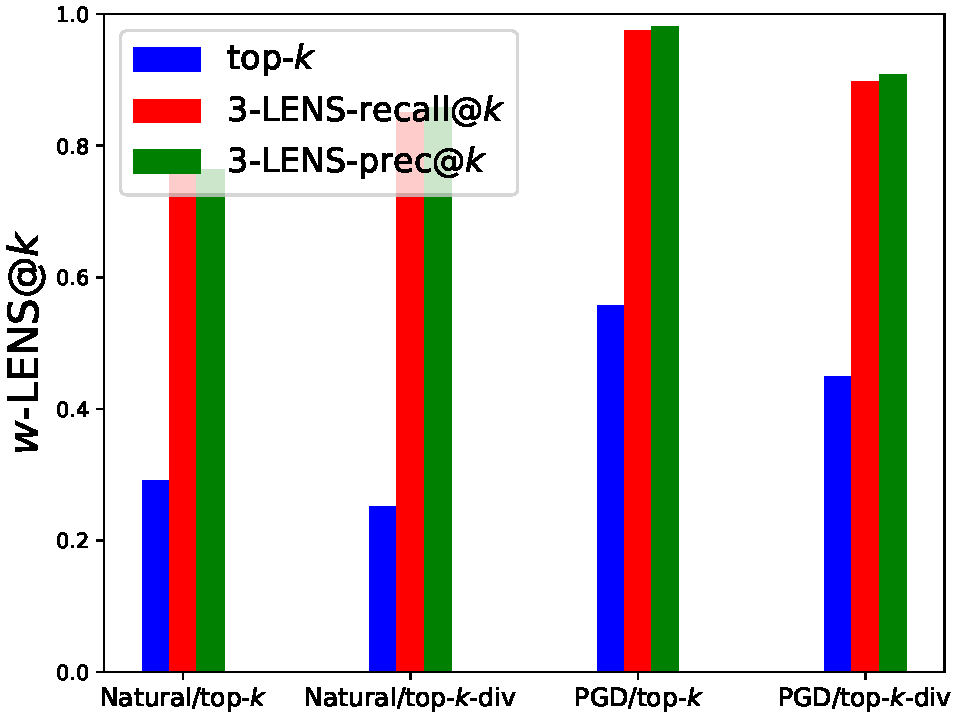
\includegraphics[width=1.0\textwidth]{./plots/imagenet_nat_pgd_rand_dl_lens_div_both_lens.pdf}
    \caption{ImageNet}
    \label{flower-rand-fig:d}
    \end{subfigure}
\end{subfigure}
\caption{Attributional robustness of DeepLIFT \citep{shrikumar2019learning} on naturally and PGD trained models measured as top-$w$ intersection, $w$-LENS-prec@$k$ and $w$-LENS-recall@$k$ between the {\bf DeepLIFT} of the original images and of their perturbations obtained by the random sign perturbation across different datasets.} 
\label{all-datasets-topk-div-both-lens-dl}
\end{figure}

\begin{figure}[!ht]
\centering
\begin{subfigure}[b]{1.0\textwidth}
    \begin{subfigure}[b]{0.15\textwidth}
    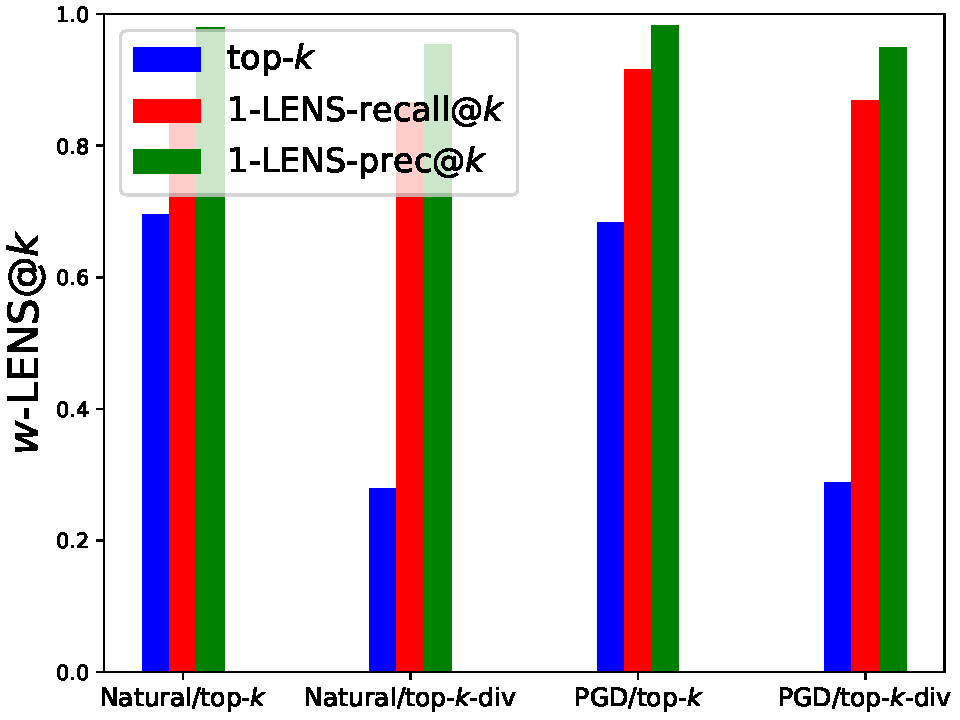
\includegraphics[width=1.0\textwidth]{./plots/mnist_nat_pgd_rand_gs_lens_div_both_lens.pdf}
    \caption{MNIST}
    \label{mnist-rand-fig:a}
    \end{subfigure}
    \begin{subfigure}[b]{0.15\textwidth}
    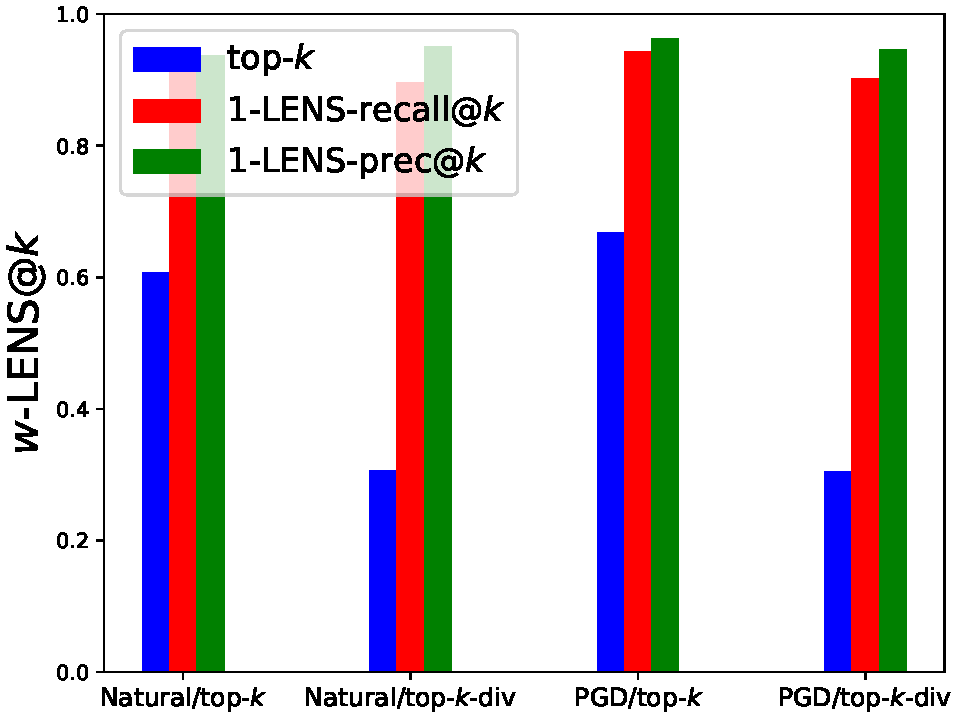
\includegraphics[width=1.0\textwidth]{./plots/fmnist_nat_pgd_rand_gs_lens_div_both_lens.pdf}
    \caption{Fashion MNIST}
    \label{fmnist-rand-fig:b}
    \end{subfigure}
    \begin{subfigure}[b]{0.15\textwidth}
    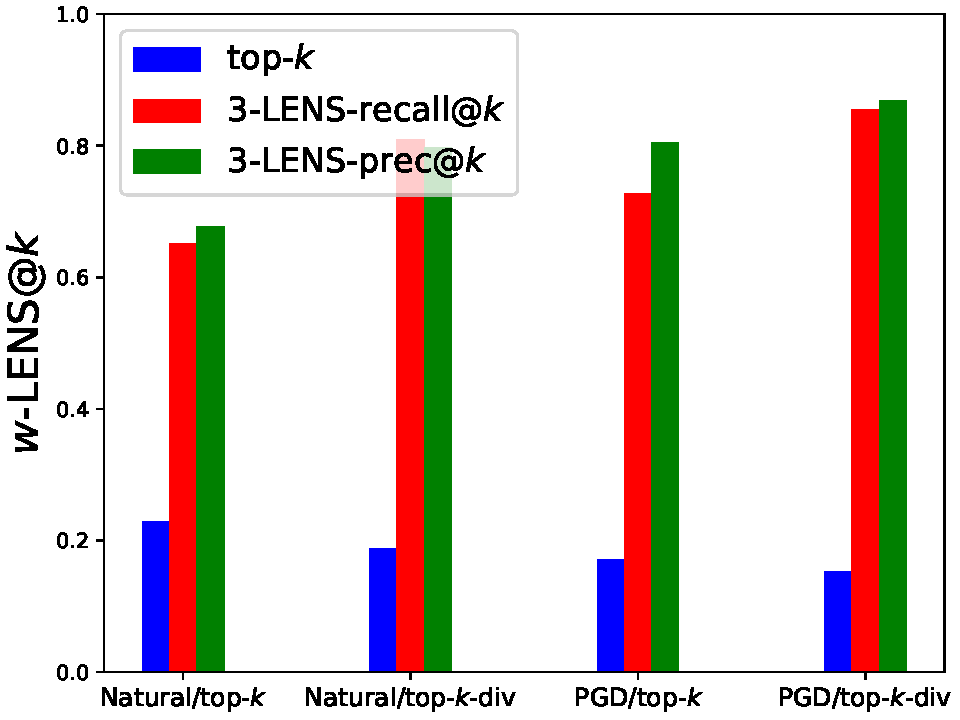
\includegraphics[width=1.0\textwidth]{./plots/imagenet_nat_pgd_rand_gs_lens_div_both_lens.pdf}
    \caption{ImageNet}
    \label{flower-rand-fig:d}
    \end{subfigure}
\end{subfigure}
\caption{Attributional robustness of GradSHAP \citep{lundberg2017unified} on naturally and PGD trained models measured as top-$k$ intersection, $w$-LENS-prec@$k$ and $w$-LENS-recall@$k$ between the {\bf GradSHAP} of the original images and of their perturbations obtained by the random sign perturbation across different datasets.} 
\label{all-datasets-topk-div-both-lens-gs}
\end{figure}

\begin{figure}[!ht]
\centering
\begin{subfigure}[b]{1.0\textwidth}
    \begin{subfigure}[b]{0.15\textwidth}
    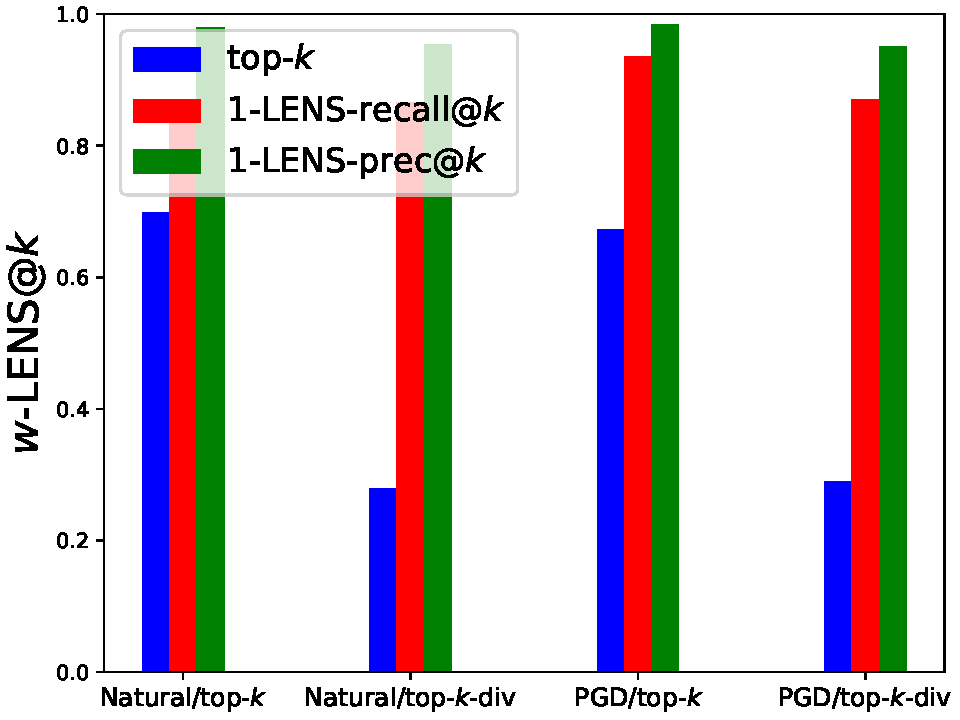
\includegraphics[width=1.0\textwidth]{./plots/mnist_nat_pgd_rand_ig_lens_div_both_lens.pdf}
    \caption{MNIST}
    \label{mnist-rand-fig:a}
    \end{subfigure}
    \begin{subfigure}[b]{0.15\textwidth}
    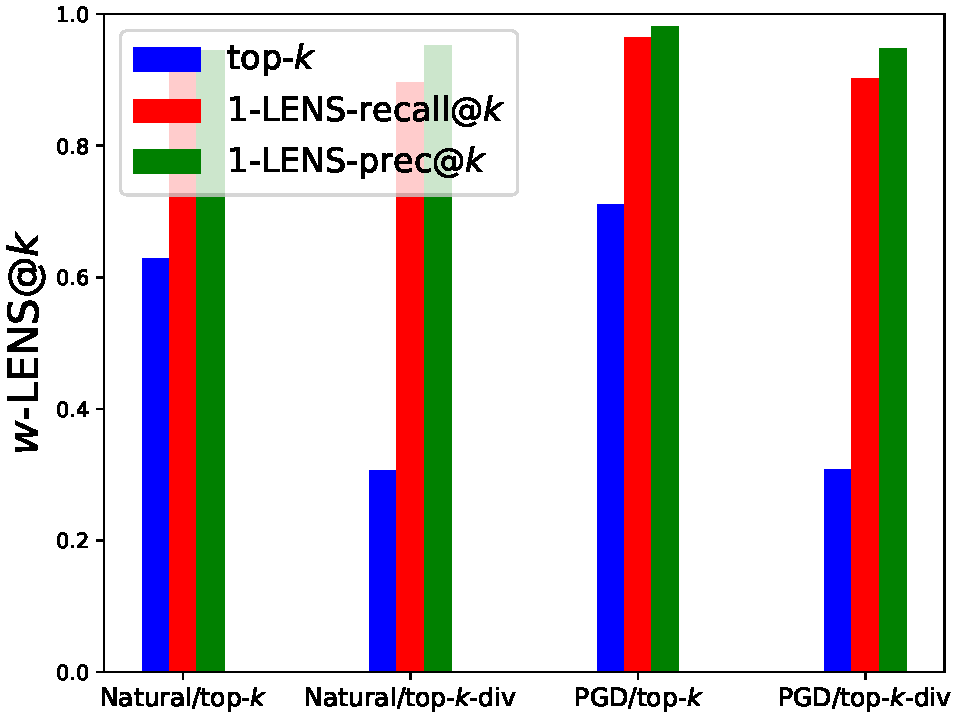
\includegraphics[width=1.0\textwidth]{./plots/fmnist_nat_pgd_rand_ig_lens_div_both_lens.pdf}
    \caption{Fashion MNIST}
    \label{fmnist-rand-fig:b}
    \end{subfigure}
    \begin{subfigure}[b]{0.15\textwidth}
    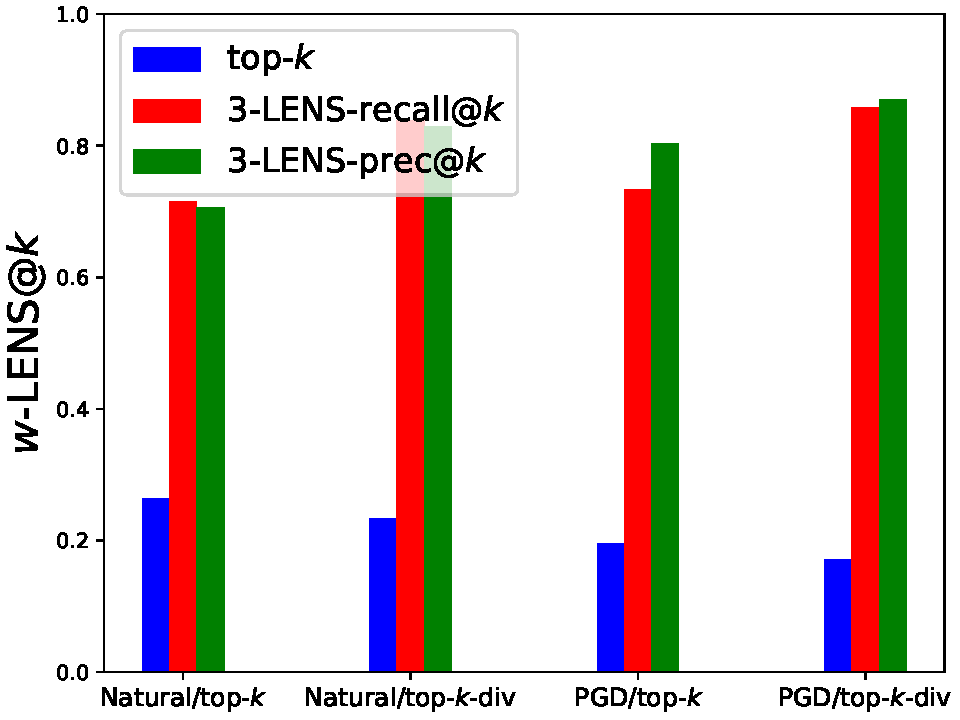
\includegraphics[width=1.0\textwidth]{./plots/imagenet_nat_pgd_rand_ig_lens_div_both_lens.pdf}
    \caption{ImageNet}
    \label{flower-rand-fig:d}
    \end{subfigure}
\end{subfigure}
\caption{Attributional robustness of Integrated Gradients \citep{SundararajanTY17} on naturally and PGD trained models measured as top-$k$ intersection, $w$-LENS-prec@$k$ and $w$-LENS-recall@$k$ between the {\bf Integrated Gradients(IG)} of the original images and of their perturbations obtained by the random sign perturbation across different datasets.} 
\label{all-datasets-topk-div-both-lens-ig}
\end{figure}

\begin{figure}[!ht]
\centering
\begin{subfigure}[b]{1.0\textwidth}
    \begin{subfigure}[b]{0.24\textwidth}
    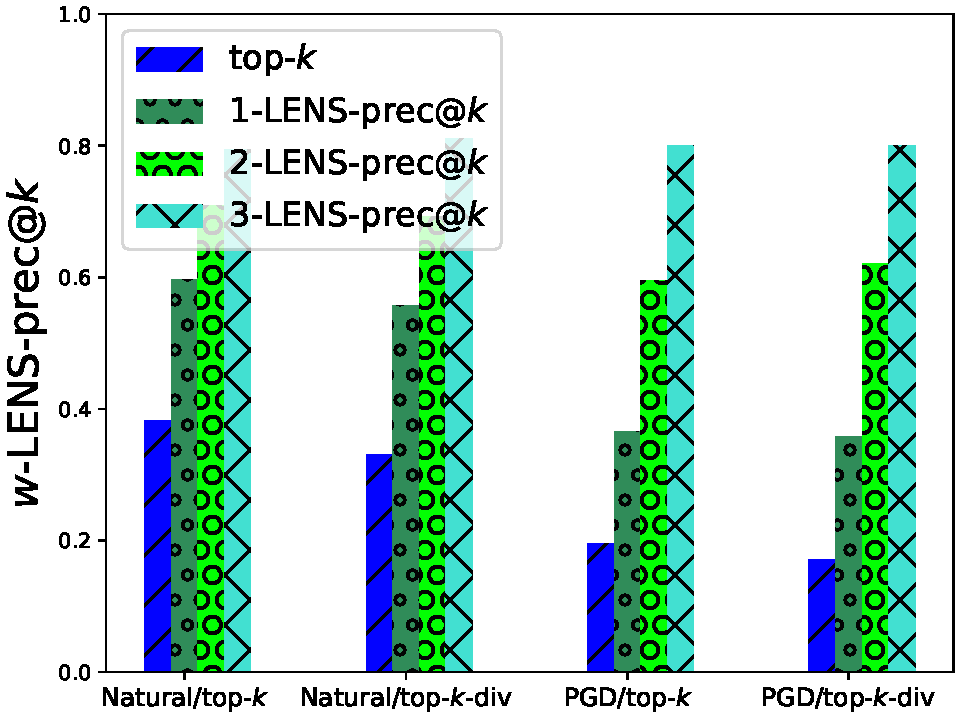
\includegraphics[width=1.0\textwidth]{./plots/imagenet_nat_pgd_rand_sg_lens_div.pdf}
    \caption{Simple Gradient}
    \label{mnist-rand-fig:a}
    \end{subfigure}
    \begin{subfigure}[b]{0.24\textwidth}
    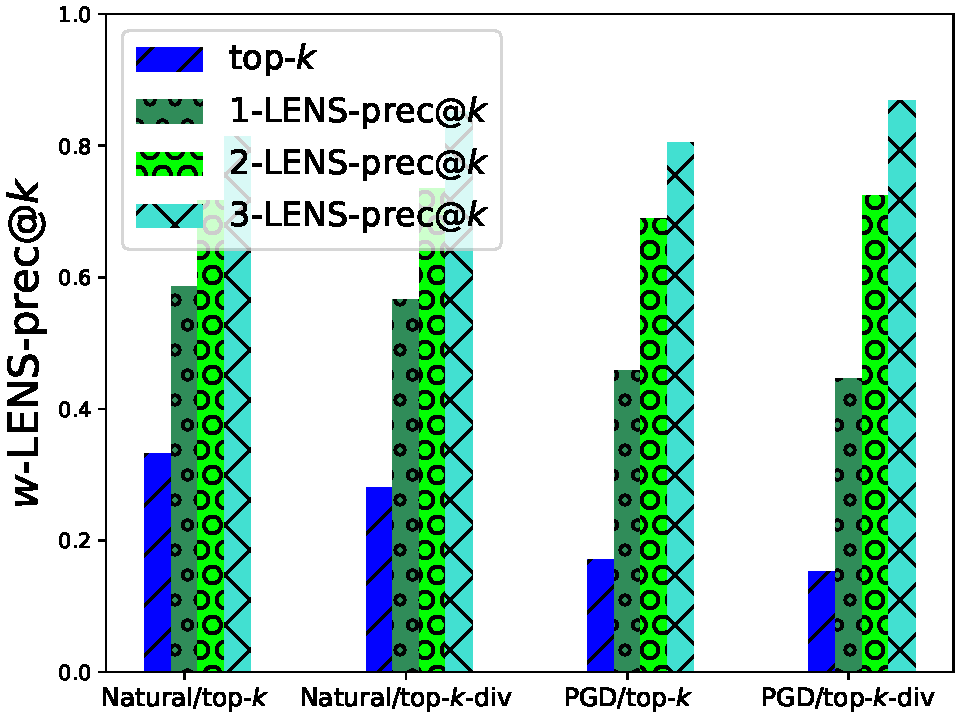
\includegraphics[width=1.0\textwidth]{./plots/imagenet_nat_pgd_rand_ixg_lens_div.pdf}
    \caption{Image $\times$ Gradient}
    \label{mnist-rand-fig:b}
    \end{subfigure}\\
    \begin{subfigure}[b]{0.24\textwidth}
    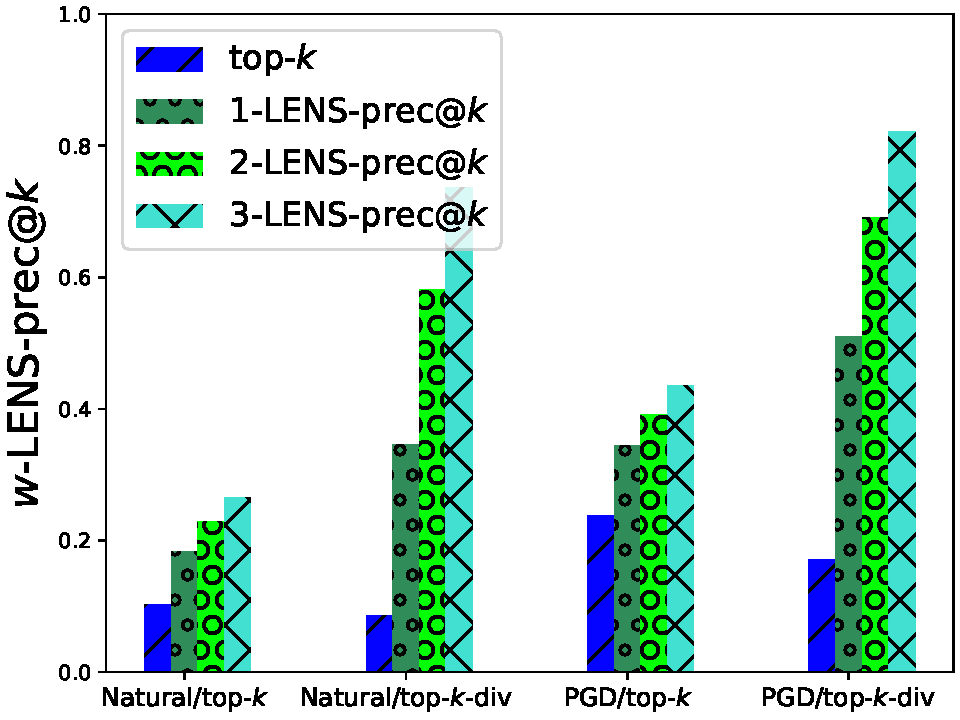
\includegraphics[width=1.0\textwidth]{./plots/imagenet_nat_pgd_rand_lrp_lens_div.pdf}
    \caption{LRP [Bach 2015]}
    \label{mnist-rand-fig:c}
    \end{subfigure}
    \begin{subfigure}[b]{0.24\textwidth}
    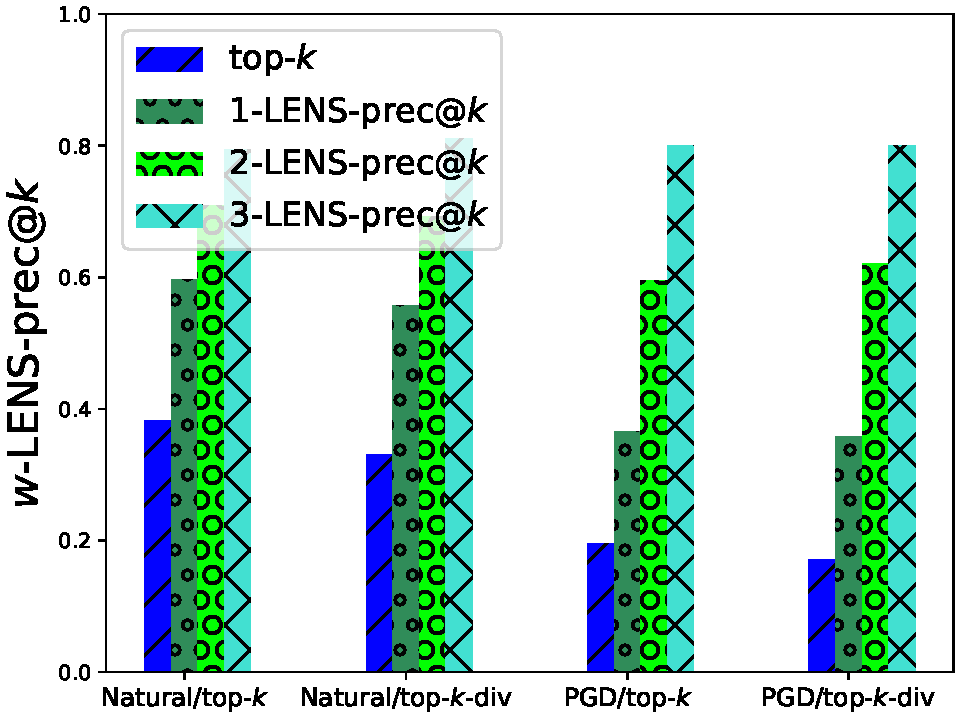
\includegraphics[width=1.0\textwidth]{./plots/imagenet_nat_pgd_rand_sg_lens_div.pdf}
    \caption{DeepLIFT [Shrikumar 2017]}
    \label{mnist-rand-fig:a}
    \end{subfigure}\\    
    \begin{subfigure}[b]{0.24\textwidth}
    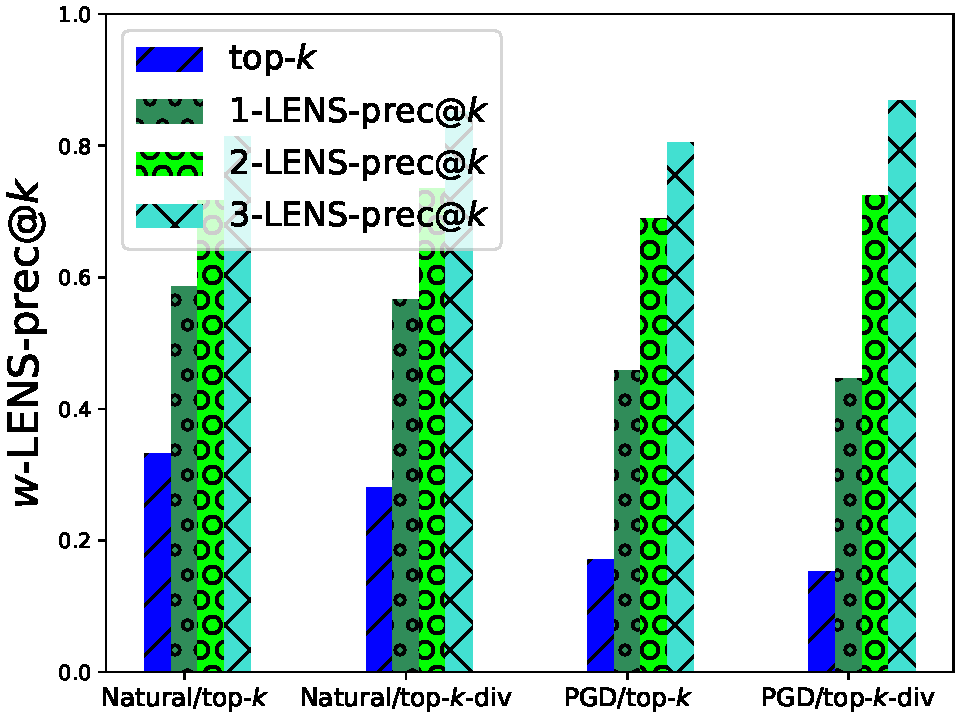
\includegraphics[width=1.0\textwidth]{./plots/imagenet_nat_pgd_rand_ixg_lens_div.pdf}
    \caption{GradSHAP [Lundberg 2017]}
    \label{mnist-rand-fig:b}
    \end{subfigure}
    \begin{subfigure}[b]{0.24\textwidth}
    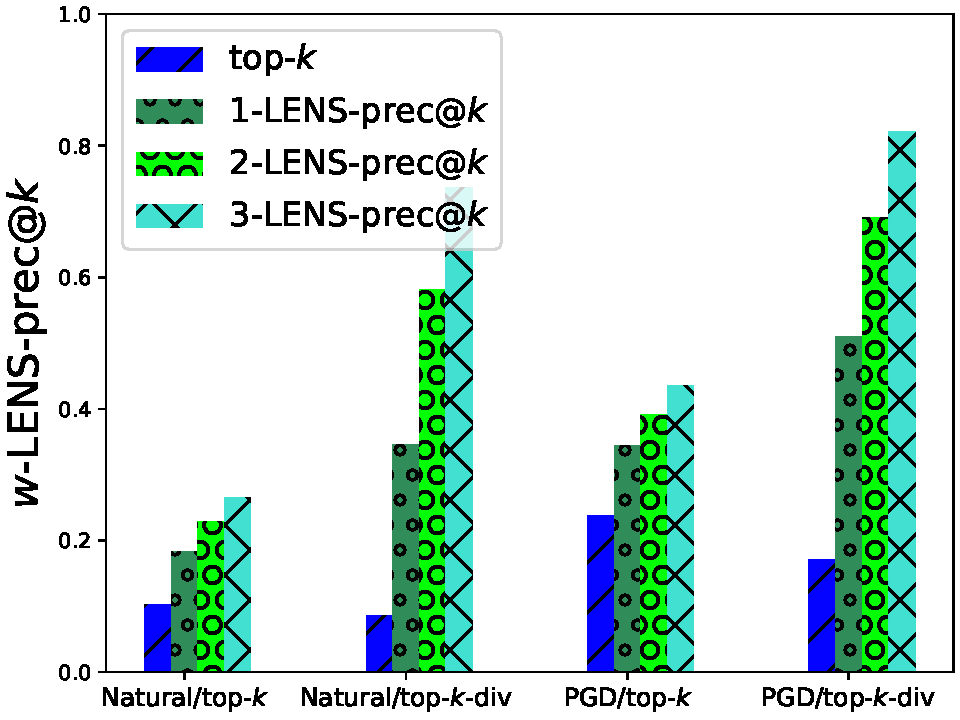
\includegraphics[width=1.0\textwidth]{./plots/imagenet_nat_pgd_rand_lrp_lens_div.pdf}
    \caption{IG [Sundararajan 2017]}
    \label{mnist-rand-fig:c}
    \end{subfigure}
\end{subfigure}
\caption{Attributional robustness of explanation methods on naturally and PGD trained models measured as top-$k$ intersection and $w$-LENS-prec@$k$ between the explanation map of the original images and their perturbations. Perturbations are obtained by the random sign perturbation. The plots show the effect of varying $w$ on ImageNet dataset with naturally and PGD trained ResNet50 model.}
\label{imagenet-nat-pgd-w-lens-div}     
\end{figure}

\clearpage

\section{The fragility of top-$k$ intersection} \label{app:sample-fragility-examples}

Figure \ref{app:flower-topk-highlight} highlights the top-100 pixels in the unperturbed and perturbed maps of a sample image. Figure \ref{app:flower-topk-highlight-lens-19}, \ref{app:flower-topk-highlight-div-19} show the top-1000 pixels and top-1000 diverse pixels along with $w$-LENS-recall@$k$ and $w$-LENS-prec@$k$ on them. Figure \ref{app:flower-topk-highlight-div-win-19} visualize the top-1000 diverse pixels obtained with different window sizes eg. 3 and 5, respectively. Figure \ref{app:imagenet-topk-highlight-loc-19} elaborates the use of LENS(locality) and Figure \ref{app:imagenet-topk-highlight-div-win-19} shows LENS-div(diversity) for the same example from ImageNet. Zoom in required to observe the finer details.

\begin{figure*}[!ht]
\centering
\begin{subfigure}[b]{1.0\textwidth}
    \begin{subfigure}[b]{0.22\textwidth}
    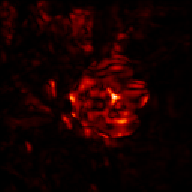
\includegraphics[width=1.0\textwidth]{./images/flower_20_topk_nat_orig.pdf}
    \caption{Original IG}
    \label{mnist-rand-fig:a}
    \end{subfigure}
    \begin{subfigure}[b]{0.22\textwidth}
    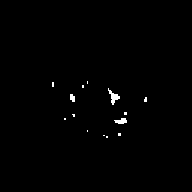
\includegraphics[width=1.0\textwidth]{./images/flower_20_topk_100_orig.pdf}
    \caption{top-100 pixels}
    \label{fmnist-rand-fig:b}
    \end{subfigure}
    \begin{subfigure}[b]{0.22\textwidth}
    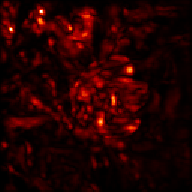
\includegraphics[width=1.0\textwidth]{./images/flower_20_topk_nat_pert.pdf}
    \caption{Perturbed IG}
    \label{gtsrb-rand-fig:c}
    \end{subfigure}
    \begin{subfigure}[b]{0.22\textwidth}
    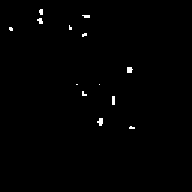
\includegraphics[width=1.0\textwidth]{./images/flower_20_topk_100_pert.pdf}
    \caption{top-100 pixels}
    \label{flower-rand-fig:d}
    \end{subfigure}
\end{subfigure}
\begin{subfigure}[b]{1.0\textwidth}
    \begin{subfigure}[b]{0.22\textwidth}
    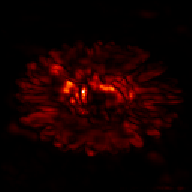
\includegraphics[width=1.0\textwidth]{./images/flower_19_topk_nat_orig.pdf}
    \caption{Original IG}
    \label{mnist-rand-fig:a}
    \end{subfigure}
    \begin{subfigure}[b]{0.22\textwidth}
    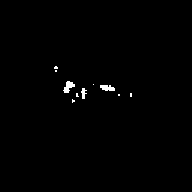
\includegraphics[width=1.0\textwidth]{./images/flower_19_topk_100_orig.pdf}
    \caption{top-100 pixels}
    \label{fmnist-rand-fig:b}
    \end{subfigure}
    \begin{subfigure}[b]{0.22\textwidth}
    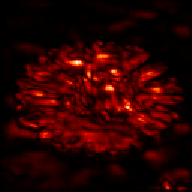
\includegraphics[width=1.0\textwidth]{./images/flower_19_topk_nat_pert.pdf}
    \caption{Perturbed IG}
    \label{gtsrb-rand-fig:c}
    \end{subfigure}
    \begin{subfigure}[b]{0.22\textwidth}
    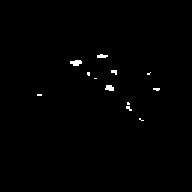
\includegraphics[width=1.0\textwidth]{./images/flower_19_topk_100_pert.pdf}
    \caption{top-100 pixels}
    \label{flower-rand-fig:d}
    \end{subfigure}    
\end{subfigure}
\caption{Sample Integrated Gradients(IG) map using Flower dataset where top-100 is highlighted before and after image is perturbed with top-$k$ attack of \citet{ghorbani2018interpretation}.}
\label{app:flower-topk-highlight}     
\end{figure*}

\begin{figure*}[!ht]
\centering
\begin{subfigure}[b]{1.0\textwidth}
    \begin{subfigure}[b]{0.22\textwidth}
    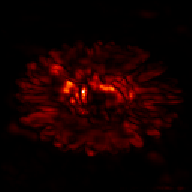
\includegraphics[width=1.0\textwidth]{./images/flower_19_topk_nat_orig.pdf}
    \caption{Original IG}
    \label{mnist-rand-fig:a}
    \end{subfigure}
    \begin{subfigure}[b]{0.22\textwidth}
    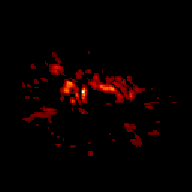
\includegraphics[width=1.0\textwidth]{./images/flower_19_topk_nat_orig_orig.pdf}
    \caption{top-1000 pixels}
    \label{fmnist-rand-fig:b}
    \end{subfigure}
    \begin{subfigure}[b]{0.22\textwidth}
    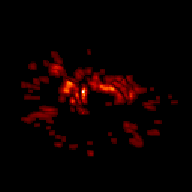
\includegraphics[width=1.0\textwidth]{./images/flower_19_topk_nat_orig_lens_rec.pdf}
    \caption{1-LENS-recall@$k$}
    \label{gtsrb-rand-fig:c}
    \end{subfigure}
    \begin{subfigure}[b]{0.22\textwidth}
    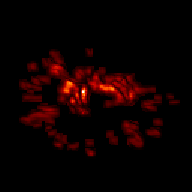
\includegraphics[width=1.0\textwidth]{./images/flower_19_topk_nat_orig_2lens_rec.pdf}
    \caption{2-LENS-recall@$k$}
    \label{flower-rand-fig:d}
    \end{subfigure}
\end{subfigure}
\begin{subfigure}[b]{1.0\textwidth}
    \begin{subfigure}[b]{0.22\textwidth}
    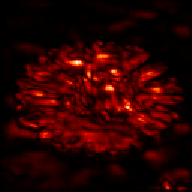
\includegraphics[width=1.0\textwidth]{./images/flower_19_topk_nat_pert.pdf}
    \caption{Perturbed IG}
    \label{mnist-rand-fig:a}
    \end{subfigure}
    \begin{subfigure}[b]{0.22\textwidth}
    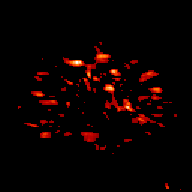
\includegraphics[width=1.0\textwidth]{./images/flower_19_topk_nat_orig_pert.pdf}
    \caption{top-1000 pixels}
    \label{fmnist-rand-fig:b}
    \end{subfigure}
    \begin{subfigure}[b]{0.22\textwidth}
    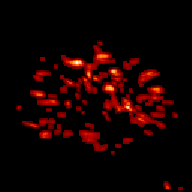
\includegraphics[width=1.0\textwidth]{./images/flower_19_topk_nat_orig_lens_pre.pdf}
    \caption{1-LENS-prec@$k$}
    \label{gtsrb-rand-fig:c}
    \end{subfigure}
    \begin{subfigure}[b]{0.22\textwidth}
    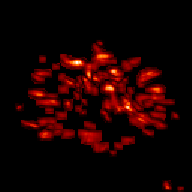
\includegraphics[width=1.0\textwidth]{./images/flower_19_topk_nat_orig_2lens_pre.pdf}
    \caption{2-LENS-prec@$k$}
    \label{flower-rand-fig:d}
    \end{subfigure}
\end{subfigure}
\caption{Example based on locality. Sample Integrated Gradients(IG) map using Flower dataset with top-$k$ highlighted followed by $w$-LENS@$k$ maps (row 1) Original IG and (row 2) Perturbed IG with top-$k$ attack \citep{ghorbani2018interpretation}.}
\label{app:flower-topk-highlight-lens-19}     
\end{figure*}

\begin{figure*}[!ht]
\centering
\begin{subfigure}[b]{1.0\textwidth}
    \begin{subfigure}[b]{0.22\textwidth}
    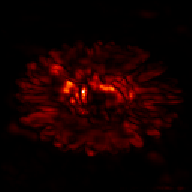
\includegraphics[width=1.0\textwidth]{./images/flower_19_topk_nat_orig.pdf}
    \caption{Original IG}
    \label{mnist-rand-fig:a}
    \end{subfigure}
    \begin{subfigure}[b]{0.22\textwidth}
    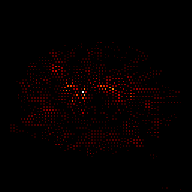
\includegraphics[width=1.0\textwidth]{./images/flower_19_topk_nat_orig_orig_div.pdf}
    \caption{top-1000-div pixels}
    \label{fmnist-rand-fig:b}
    \end{subfigure}
    \begin{subfigure}[b]{0.22\textwidth}
    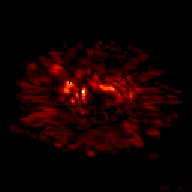
\includegraphics[width=1.0\textwidth]{./images/flower_19_topk_nat_orig_lens_rec_div.pdf}
    \caption{1-LENS-recall@$k$-div}
    \label{gtsrb-rand-fig:c}
    \end{subfigure}
    \begin{subfigure}[b]{0.22\textwidth}
    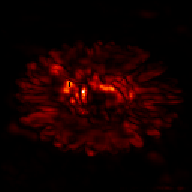
\includegraphics[width=1.0\textwidth]{./images/flower_19_topk_nat_orig_2lens_rec_div.pdf}
    \caption{2-LENS-recall@$k$-div}
    \label{flower-rand-fig:d}
    \end{subfigure}
\end{subfigure}
\begin{subfigure}[b]{1.0\textwidth}
    \begin{subfigure}[b]{0.22\textwidth}
    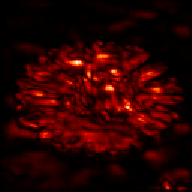
\includegraphics[width=1.0\textwidth]{./images/flower_19_topk_nat_pert.pdf}
    \caption{Perturbed IG}
    \label{mnist-rand-fig:a}
    \end{subfigure}
    \begin{subfigure}[b]{0.22\textwidth}
    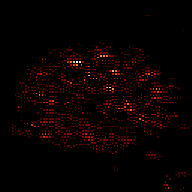
\includegraphics[width=1.0\textwidth]{./images/flower_19_topk_nat_orig_pert_div.pdf}
    \caption{top-1000-div pixels}
    \label{fmnist-rand-fig:b}
    \end{subfigure}
    \begin{subfigure}[b]{0.22\textwidth}
    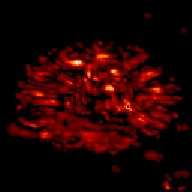
\includegraphics[width=1.0\textwidth]{./images/flower_19_topk_nat_orig_lens_pre_div.pdf}
    \caption{1-LENS-prec@$k$-div}
    \label{gtsrb-rand-fig:c}
    \end{subfigure}
    \begin{subfigure}[b]{0.22\textwidth}
    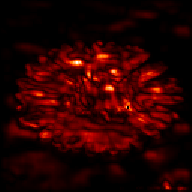
\includegraphics[width=1.0\textwidth]{./images/flower_19_topk_nat_orig_2lens_pre_div.pdf}
    \caption{2-LENS-prec@$k$-div}
    \label{flower-rand-fig:d}
    \end{subfigure}
\end{subfigure}
\caption{Example based on diversity. Sample Integrated Gradients(IG) map using Flower dataset with top-$k$-div highlighted followed by $w$-LENS@$k$-div maps (row 1) Original IG and (row 2) Perturbed IG with top-$k$ attack \citep{ghorbani2018interpretation}.}
\label{app:flower-topk-highlight-div-19}     
\end{figure*}

\begin{comment}    

\begin{figure*}[!ht]
\centering
\begin{subfigure}[b]{1.0\textwidth}
    \begin{subfigure}[b]{0.22\textwidth}
    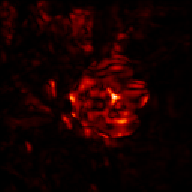
\includegraphics[width=1.0\textwidth]{./images/flower_20_topk_nat_orig.pdf}
    \caption{Original IG}
    \label{mnist-rand-fig:a}
    \end{subfigure}
    \begin{subfigure}[b]{0.22\textwidth}
    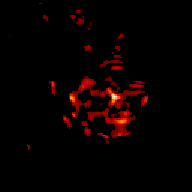
\includegraphics[width=1.0\textwidth]{./images/flower_20_topk_nat_orig_orig.pdf}
    \caption{top-1000 pixels}
    \label{fmnist-rand-fig:b}
    \end{subfigure}
    \begin{subfigure}[b]{0.22\textwidth}
    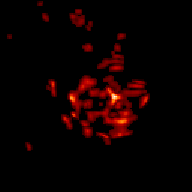
\includegraphics[width=1.0\textwidth]{./images/flower_20_topk_nat_orig_lens_rec.pdf}
    \caption{1-LENS-recall@$k$}
    \label{gtsrb-rand-fig:c}
    \end{subfigure}
    \begin{subfigure}[b]{0.22\textwidth}
    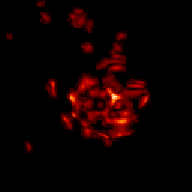
\includegraphics[width=1.0\textwidth]{./images/flower_20_topk_nat_orig_2lens_rec.pdf}
    \caption{2-LENS-recall@$k$}
    \label{flower-rand-fig:d}
    \end{subfigure}
\end{subfigure}
\begin{subfigure}[b]{1.0\textwidth}
    \begin{subfigure}[b]{0.22\textwidth}
    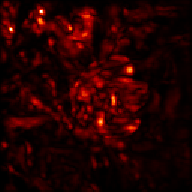
\includegraphics[width=1.0\textwidth]{./images/flower_20_topk_nat_pert.pdf}
    \caption{Perturbed IG}
    \label{mnist-rand-fig:a}
    \end{subfigure}
    \begin{subfigure}[b]{0.22\textwidth}
    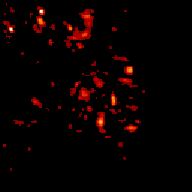
\includegraphics[width=1.0\textwidth]{./images/flower_20_topk_nat_orig_pert.pdf}
    \caption{top-1000 pixels}
    \label{fmnist-rand-fig:b}
    \end{subfigure}
    \begin{subfigure}[b]{0.22\textwidth}
    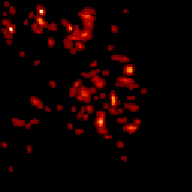
\includegraphics[width=1.0\textwidth]{./images/flower_20_topk_nat_orig_lens_pre.pdf}
    \caption{1-LENS-prec@$k$}
    \label{gtsrb-rand-fig:c}
    \end{subfigure}
    \begin{subfigure}[b]{0.22\textwidth}
    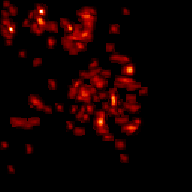
\includegraphics[width=1.0\textwidth]{./images/flower_20_topk_nat_orig_2lens_pre.pdf}
    \caption{2-LENS-prec@$k$}
    \label{flower-rand-fig:d}
    \end{subfigure}
\end{subfigure}
\caption{Example with only Locality. Sample top-$k$ highlighting using Flower with (row 1) Original IG and (row 2) Perturbed IG.}
\label{app:flower-topk-highlight-lens-20}     
\end{figure*}

\begin{figure*}[!ht]
\centering
\begin{subfigure}[b]{1.0\textwidth}
    \begin{subfigure}[b]{0.22\textwidth}
    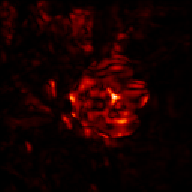
\includegraphics[width=1.0\textwidth]{./images/flower_20_topk_nat_orig.pdf}
    \caption{Original IG}
    \label{mnist-rand-fig:a}
    \end{subfigure}
    \begin{subfigure}[b]{0.22\textwidth}
    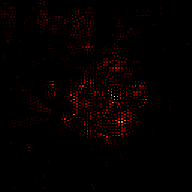
\includegraphics[width=1.0\textwidth]{./images/flower_20_topk_nat_orig_orig_div.pdf}
    \caption{top-1000-div pixels}
    \label{fmnist-rand-fig:b}
    \end{subfigure}
    \begin{subfigure}[b]{0.22\textwidth}
    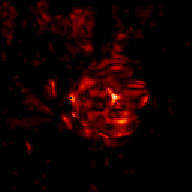
\includegraphics[width=1.0\textwidth]{./images/flower_20_topk_nat_orig_lens_rec_div.pdf}
    \caption{1-LENS-recall@$k$-div}
    \label{gtsrb-rand-fig:c}
    \end{subfigure}
    \begin{subfigure}[b]{0.22\textwidth}
    \includegraphics[width=1.0\textwidth]{./images/flower_20_topk_nat_orig_2lens_rec_div.pdf}
    \caption{2-LENS-recall@$k$-div}
    \label{flower-rand-fig:d}
    \end{subfigure}
\end{subfigure}
\begin{subfigure}[b]{1.0\textwidth}
    \begin{subfigure}[b]{0.22\textwidth}
    \includegraphics[width=1.0\textwidth]{./images/flower_20_topk_nat_pert.pdf}
    \caption{Perturbed IG}
    \label{mnist-rand-fig:a}
    \end{subfigure}
    \begin{subfigure}[b]{0.22\textwidth}
    \includegraphics[width=1.0\textwidth]{./images/flower_20_topk_nat_orig_pert_div.pdf}
    \caption{top-1000-div pixels}
    \label{fmnist-rand-fig:b}
    \end{subfigure}
    \begin{subfigure}[b]{0.22\textwidth}
    \includegraphics[width=1.0\textwidth]{./images/flower_20_topk_nat_orig_lens_pre_div.pdf}
    \caption{1-LENS-prec@$k$-div}
    \label{gtsrb-rand-fig:c}
    \end{subfigure}
    \begin{subfigure}[b]{0.22\textwidth}
    \includegraphics[width=1.0\textwidth]{./images/flower_20_topk_nat_orig_2lens_pre_div.pdf}
    \caption{2-LENS-prec@$k$-div}
    \label{flower-rand-fig:d}
    \end{subfigure}
\end{subfigure}
\caption{Example with Diversity and Locality. Sample top-$k$ highlighting using Flower with (row 1) Original IG and (row 2) Perturbed IG.}
\label{app:flower-topk-highlight-div-20}     
\end{figure*}
\end{comment}

\begin{figure*}[!ht]
\centering
\begin{subfigure}[b]{1.0\textwidth}
    \begin{subfigure}[b]{0.33\textwidth}
    \includegraphics[width=1.0\textwidth]{./images/flower_19_topk_nat_orig.pdf}
    \caption{Original IG}
    \label{mnist-rand-fig:a}
    \end{subfigure}
    \begin{subfigure}[b]{0.33\textwidth}
    \includegraphics[width=1.0\textwidth]{./images/flower_19_topk_nat_orig_orig_div.pdf}
    \caption{top-1000 diverse pixels with $3{\times}3$ window}
    \label{fmnist-rand-fig:b}
    \end{subfigure}
    \begin{subfigure}[b]{0.33\textwidth}
    \includegraphics[width=1.0\textwidth]{./images/flower_19_topk_nat_orig_orig_2div.pdf}
    \caption{top-1000 diverse pixels with $5{\times}5$ window}
    \label{gtsrb-rand-fig:c}
    \end{subfigure}
    %\begin{subfigure}[b]{0.22\textwidth}
    %\includegraphics[width=1.0\textwidth]{./images/flower_19_topk_nat_orig_2lens_pre.pdf}
    %\caption{2-LENS-prec@$k$}
    %\label{flower-rand-fig:d}
    %\end{subfigure}
\end{subfigure}
\begin{subfigure}[b]{1.0\textwidth}
    \begin{subfigure}[b]{0.33\textwidth}
    \includegraphics[width=1.0\textwidth]{./images/flower_19_topk_nat_pert.pdf}
    \caption{Perturbed IG}
    \label{mnist-rand-fig:a}
    \end{subfigure}
    \begin{subfigure}[b]{0.33\textwidth}
    \includegraphics[width=1.0\textwidth]{./images/flower_19_topk_nat_orig_pert_div.pdf}
    \caption{top-1000 diverse pixels with $3{\times}3$ window}
    \label{fmnist-rand-fig:b}
    \end{subfigure}
    \begin{subfigure}[b]{0.33\textwidth}
    \includegraphics[width=1.0\textwidth]{./images/flower_19_topk_nat_orig_pert_2div.pdf}
    \caption{top-1000 diverse pixels with $5{\times}5$ window}
    \label{gtsrb-rand-fig:c}
    \end{subfigure}
    %\begin{subfigure}[b]{0.22\textwidth}
    %\includegraphics[width=1.0\textwidth]{./images/flower_19_topk_nat_orig_2lens_pre.pdf}
    %\caption{2-LENS-prec@$k$}
    %\label{flower-rand-fig:d}
    %\end{subfigure}
\end{subfigure}
\caption{Example based on diversity with different window sizes. Sample Integrated Gradients(IG) map using Flower dataset with top-$k$-div highlighted with (column 2) 3$\times$3 window (column 3) 5$\times$5 window. (column 1) (top) map of unperturbed image (bottom) map of perturbed image with top-$k$ attack \citep{ghorbani2018interpretation}.}
\label{app:flower-topk-highlight-div-win-19}     
\end{figure*}

\begin{figure*}[!ht]
\centering
\begin{subfigure}[b]{1.0\textwidth}
    \begin{subfigure}[b]{0.24\textwidth}
    \includegraphics[width=1.0\textwidth]{./images/imagenet_19.pdf}
    \caption{Original Image}
    \label{mnist-rand-fig:a}
    \end{subfigure}
    \begin{subfigure}[b]{0.24\textwidth}
    \includegraphics[width=1.0\textwidth]{./images/imagenet_19_orig_topk.pdf}
    \caption{top-1000 of Original IG}
    \label{mnist-rand-fig:a}
    \end{subfigure}  
    \begin{subfigure}[b]{0.24\textwidth}
    \includegraphics[width=1.0\textwidth]{./images/imagenet_19_recall.pdf}
    \caption{3-LENS-recall@1000}
    \label{fmnist-rand-fig:b}
    \end{subfigure}
    \begin{subfigure}[b]{0.24\textwidth}
    \includegraphics[width=1.0\textwidth]{./images/imagenet_19_recall_bw.pdf}
    \caption{3-LENS-recall@1000 0/1}
    \label{fmnist-rand-fig:b}
    \end{subfigure}
\end{subfigure}
\begin{subfigure}[b]{1.0\textwidth}
    \begin{subfigure}[b]{0.24\textwidth}
    \includegraphics[width=1.0\textwidth]{./images/imagenet_19_pert_img.pdf}
    \caption{Perturbed Image}
    \label{mnist-rand-fig:a}
    \end{subfigure}
    \begin{subfigure}[b]{0.24\textwidth}
    \includegraphics[width=1.0\textwidth]{./images/imagenet_19_pert_topk.pdf}
    \caption{top-1000 of Perturbed IG}
    \label{fmnist-rand-fig:b}
    \end{subfigure}    
    \begin{subfigure}[b]{0.24\textwidth}
    \includegraphics[width=1.0\textwidth]{./images/imagenet_19_prec.pdf}
    \caption{3-LENS-prec@1000}
    \label{gtsrb-rand-fig:c}
    \end{subfigure}    
        \begin{subfigure}[b]{0.24\textwidth}
    \includegraphics[width=1.0\textwidth]{./images/imagenet_19_prec_bw.pdf}
    \caption{3-LENS-prec@1000 0/1}
    \label{gtsrb-rand-fig:c}
    \end{subfigure}
\end{subfigure}    
\caption{Example based on locality(LENS) with sample Integrated Gradients(IG) map from ImageNet dataset (a) the original image and (b) being the perturbed image. (c) and (d) show top-$k$ highlighted and (e) and (f) are the corresponding maps with LENS. Maps (g), (h) are the maps corresponding to (e), (f), respectively with non-zero value pixels shown as white. top-k:0.108, 3-LENS-recall@k:0.254, 3-LENS-prec@k:0.433, top-k-div:0.090, 3-LENS-recall@k-div:0.758, 3-LENS-prec@k-div:0.807}
\label{app:imagenet-topk-highlight-loc-19}     
\end{figure*}

\begin{figure*}[!ht]
\centering
\begin{subfigure}[b]{1.0\textwidth}
    \begin{subfigure}[b]{0.24\textwidth}
    \includegraphics[width=1.0\textwidth]{./images/imagenet_19_orig.pdf}
    \caption{Original IG}
    \label{mnist-rand-fig:a}
    \end{subfigure}
    \begin{subfigure}[b]{0.24\textwidth}
    \includegraphics[width=1.0\textwidth]{./images/imagenet_19_div_orig.pdf}
    \caption{top-1000-div of Original IG}
    \label{mnist-rand-fig:a}
    \end{subfigure}
    \begin{subfigure}[b]{0.24\textwidth}
    \includegraphics[width=1.0\textwidth]{./images/imagenet_19_div_recall.pdf}
    \caption{3-LENS-recall@1000-div}
    \label{fmnist-rand-fig:b}
    \end{subfigure}
    \begin{subfigure}[b]{0.24\textwidth}
    \includegraphics[width=1.0\textwidth]{./images/imagenet_19_div_recall_bw.pdf}
    \caption{3-LENS-recall@1000-div 0/1}
    \label{fmnist-rand-fig:b}
    \end{subfigure}
\end{subfigure}
\begin{subfigure}[b]{1.0\textwidth}
    \begin{subfigure}[b]{0.24\textwidth}
    \includegraphics[width=1.0\textwidth]{./images/imagenet_19_pert.pdf}
    \caption{Perturbed IG}
    \label{mnist-rand-fig:a}
    \end{subfigure}    
    \begin{subfigure}[b]{0.24\textwidth}
    \includegraphics[width=1.0\textwidth]{./images/imagenet_19_div_pert.pdf}
    \caption{top-1000-div of Perturbed IG}
    \label{fmnist-rand-fig:b}
    \end{subfigure}
    \begin{subfigure}[b]{0.24\textwidth}
    \includegraphics[width=1.0\textwidth]{./images/imagenet_19_div_prec.pdf}
    \caption{3-LENS-prec@1000-div}
    \label{gtsrb-rand-fig:c}
    \end{subfigure}    
    \begin{subfigure}[b]{0.24\textwidth}
    \includegraphics[width=1.0\textwidth]{./images/imagenet_19_div_prec_bw.pdf}
    \caption{3-LENS-prec@1000-div 0/1}
    \label{gtsrb-rand-fig:c}
    \end{subfigure}
\end{subfigure}
\caption{Example based on diversity with 7$\times$7 window size with sample Integrated Gradients(IG) map from ImageNet dataset (a) the original IG of unperturbed image and (b) perturbed IG obtained with top-$k$ attack\citep{ghorbani2018interpretation}. (c) and (d) show top-$k$-div highlighted and (e) and (f) are the corresponding maps with LENS. Maps (g), (h) are the maps corresponding to (e), (f), respectively with non-zero value pixels shown as white. top-k:0.108, 3-LENS-recall@k:0.254, 3-LENS-prec@k:0.433, top-k-div:0.090, 3-LENS-recall@k-div:0.758, 3-LENS-prec@k-div:0.807}
\label{app:imagenet-topk-highlight-div-win-19}     
\end{figure*}

\clearpage

\section{Additional results for PGD-trained and IG-SUM-NORM trained models} \label{app:pgd-rar-results}

%\textcolor{blue}{Just point to other sections do not remove as the section names will change in main paper.}
Figure \ref{dataset-topk-rand-diff-k-new-metric-pgd} and Figure \ref{dataset-topk-rand-diff-k-new-metric-rar} shows the impact of $k$ in top-$k$ for adversarially(PGD) trained and attributional(IG-SUM-NORM) trained network, respectively. But an important point to be noticed is that even with small number of features LENS is able to cross 70-80\% which supports the observation of sparsity and stability of attributions achieved by adversarially(PGD) trained models by \citet{ChalasaniC00J20}. Similarly, the experiments with different $w$ value for $w$-LENS-top-$k$ in Figure \ref{flower-topk-new-metric-training-method} clearly incidates that due to the stability properties at lower window sizes LENS is able to cross the 80\% intersection quickly. Supporting that our metric nicely captures local stability very well. 

While above we observed only the top-$k$ version of LENS. Figure \ref{dataset-smooth-sp-ken-nat-pgd-rar} further extends the observation to LENS-Spearman and LENS-Kendall who to show that with LENS with a smoothing of $3 \times 3$ the maps from PGD-trained and IG-SUM-NORM trained models have a higher top-$k$ intersection above 70\% in comparison to natural trained model across all datasets used in our experiments, which further strengthen the conclusions from previous papers that IG on PGD-trained and IG-SUM-NORM trained models give better attributions.

Appendix \ref{app:more-lens-results} and \ref{app:extra-div-results} provide results on PGD-trained and IG-SUM-NORM trained models along with naturally trained models for compact presentation of results.
%The above observation about robustness of Integrated Gradients (IG) for PGD-trained and IG-SUM-NORM trained models holds even when we use $1$-LENS-Spearman and $1$-LENS-Kendall measures to quantify the attributional robustness to the top-$k$ attack of \citet{ghorbani2018interpretation}, and it holds across all datasets used in our experiments; see Figure \ref{dataset-smooth-sp-ken-nat-pgd-rar}. Moreover, the $1$-LENS-Kendall and $1$-LENS-Spearman values in Figure \ref{dataset-smooth-sp-ken-nat-pgd-rar} are always higher than the corresponding Kendall's $\tau$ and Spearman's $\rho$ values, which further strengthen the conclusions from previous papers that IG on PGD-trained and IG-SUM-NORM trained models give better attributions.

%\begin{figure*}[!ht]
%\centering
%\begin{subfigure}[b]{1.0\textwidth}
%    \begin{subfigure}[b]{0.33\textwidth}
%    \includegraphics[width=1.0\textwidth]{./plots/flower_topk_attack_new_metric_ig.pdf}
%    \caption{IG : top-$k$}
%    \label{mnist-rand-fig:a}
%    \end{subfigure}
%    \begin{subfigure}[b]{0.33\textwidth}
%    \includegraphics[width=1.0\textwidth]{./plots/flower_random_attack_new_metric_ig.pdf}
%    \caption{IG : random}
%    \label{mnist-rand-fig:b}
%    \end{subfigure}
%    \begin{subfigure}[b]{0.33\textwidth}
%    \includegraphics[width=1.0\textwidth]{./plots/flower_mc_attack_new_metric_ig.pdf}
%    \caption{IG : center of mass}
%    \label{mnist-rand-fig:c}
%    \end{subfigure}
%\end{subfigure}
%\caption{Attributional robustness of IG on naturally, PGD and IG-SUM-NORM trained models measured as top-$k$ intersection and $w$-LENS-prec@$k$ between the IG of the original images and the IG of their perturbations. Perturbations are obtained by the top-$t$ attack and the mass-center attack \citep{ghorbani2018interpretation} as well as a random perturbation. The plots show the effect of varying $w$ on Flower dataset.}
%\label{flower-topk-window-new-metric-nat-pgd-rar-ig}     
%\end{figure*}


%\subsection{A Stronger Model for Attributional Robustness}
%\textcolor{purple}{Moved figures from section.}
%\clearpage

\section{Additional results with top-$k$-div} \label{app:extra-div-results}
Table \ref{table-topk-div-results-mnist-fmnist-ig}  provides detailed LENS and diversity with LENS results on MNIST, Fashion-MNIST, Table \ref{table-topk-div-results-flower-ig} on Flower with natural, PGD and IG-SUM-NORM trained networks and Table \ref{table-topk-div-results-imagenet-ig} on naturally trained network for ImageNet. All results with top-$k$, center of mass attack proposed by \citet{ghorbani2018interpretation} and random sign perturbation using Integrated Gradients(IG).

Table \ref{table-topk-div-results-rand-mnist-fmnist} show the LENS and diversity results with random sign perturbation on MNIST, Fashion MNIST and Table \ref{table-topk-div-results-rand-imagenet-app} on ImageNet with different explanation methods like Simple Gradients(SG), Image$\times$Gradient, DeepLIFT\citep{shrikumar2017just,shrikumar2019learning}, LRP \citep{bach2015lrp}, GradShap\citep{lundberg2017unified} and Integrated Gradients(IG) \citep{SundararajanTY17}. 

\begin{table*}[!ht]
\begin{center}
\resizebox{1.0\textwidth}{!}{ 
\begin{tabular}{|l|l|c|c|c|c|c|c|c|c|}
\hline 
%Dataset & Training & Attack & {\bf Explanation method} & {\bf topk} & {\bf 1-LENS-recall@$k$ metric(\%)} &  {\bf 1-LENS-prec@$k$ metric(\%)} & {\bf topk-div} & {\bf 1-LENS-recall-div@$k$ metric(\%)} &  {\bf 1-LENS-prec-div@$k$ metric(\%)} \\
{\bf Dataset} & {\bf Train Type} & {\bf Attack Type} & {\bf Attribution Method} & {\bf top-$k$ intersection} & {\bf 1-LENS-recall@$k$} &  {\bf 1-LENS-prec@$k$} & {\bf top-$k$-div} & {\bf 1-LENS-recall@$k$-div} &  {\bf 1-LENS-prec@$k$-div} \\
\hline
MNIST & Nat & top-$k$ & IG & 0.4635 & 0.6209 & 0.9427 & 0.1680 & 0.6592 & 0.8126 \\ 
      & Nat & mass center   & IG & 0.5779 & 0.7146 & 0.9572 & 0.1708 & 0.6183 & 0.7191 \\ 
      & Nat & random & IG & 0.7384 & 0.8790 & 0.9808 & 0.2046 & 0.6774 & 0.8140 \\ 
\hline
MNIST & PGD & top-$k$ & IG & 0.5378 & 0.6127 & 0.9690 & 0.2300 & 0.6567 & 0.8114 \\ 
      & PGD & mass center   & IG & 0.6077 & 0.7133 & 0.9700 & 0.1907 & 0.5894 & 0.6801 \\ 
      & PGD & random & IG & 0.6867 & 0.8220 & 0.9835 & 0.1751 & 0.6726 & 0.7995 \\ 
\hline
MNIST & IG-SUM-NORM & top-$k$ & IG & 0.6406 & 0.7817 & 0.9736 & 0.2327 & 0.6701 & 0.7995 \\ 
      & IG-SUM-NORM & mass center   & IG & 0.7075 & 0.8387 & 0.9695 & 0.2002 & 0.6293 & 0.7294 \\ 
      & IG-SUM-NORM & random & IG & 0.7746 & 0.9129 & 0.9846 & 0.1783 & 0.6788 & 0.8142 \\ 
\hline
Fashion-MNIST & Nat & top-$k$ & IG & 0.3841 & 0.9118 & 0.9361 & 0.2132 & 0.8404 & 0.8857 \\ 
      & Nat & mass center   & IG & 0.5624 & 0.9333 & 0.9370 & 0.2961 & 0.8034 & 0.8277 \\ 
      & Nat & random & IG & 0.5378 & 0.9377 & 0.9500 & 0.2716 & 0.8337 & 0.8825 \\ 
\hline
Fashion-MNIST & PGD & top-$k$ & IG & 0.7440 & 0.9571 & 0.9696 & 0.3770 & 0.8486 & 0.8608 \\ 
      & PGD & mass center   & IG & 0.8543 & 0.9659 & 0.9721 & 0.4323 & 0.8249 & 0.8357 \\ 
      & PGD & random & IG & 0.8816 & 0.9863 & 0.9892 & 0.3806 & 0.8451 & 0.8695 \\ 
\hline
Fashion-MNIST & IG-SUM-NORM & top-$k$ & IG & 0.6953 & 0.9608 & 0.9697 & 0.3671 & 0.8437 & 0.8655 \\ 
      & IG-SUM-NORM & mass center   & IG & 0.8630 & 0.9666 & 0.9752 & 0.4485 & 0.8278 & 0.8437 \\ 
      & IG-SUM-NORM & random & IG & 0.8733 & 0.9837 & 0.9900 & 0.3459 & 0.8444 & 0.8766 \\ 
\hline
\end{tabular}
}
%\vspace{-6pt}
\end{center}
    \caption{Table with top-$k$ intersection and top-$k$-div results for MNIST and Fashion MNIST with LeNet based model using Integrated Gradients(IG) \citep{SundararajanTY17}. The columns first contain locality results: top-$k$ intersection, 1-LENS-recall@$k$, 1-LENS-prec@$k$ followed by diversity results: top-$k$-div, 1-LENS-recall@$k$-div, 1-LENS-prec@$k$-div. Models trained naturally, PGD and IG-SUM-NORM are used. Results include top-$k$, center of mass attack of \citet{ghorbani2018interpretation} as well as random sign perturbation.}
%\vspace{-9pt}
\label{table-topk-div-results-mnist-fmnist-ig}
\end{table*}

\begin{table*}[!ht]
\begin{center}
\resizebox{1.0\textwidth}{!}{ 
\begin{tabular}{|l|l|c|c|c|c|c|c|c|c|}
\hline 
%Dataset & Training & Attack & {\bf Explanation method} & {\bf topk} & {\bf 1-LENS-recall@$k$ metric(\%)} &  {\bf 1-LENS-prec@$k$ metric(\%)} & {\bf topk-div} & {\bf 1-LENS-recall-div@$k$ metric(\%)} &  {\bf 1-LENS-prec-div@$k$ metric(\%)} \\
{\bf Dataset} & {\bf Train Type} & {\bf Attack Type} & {\bf Attribution Method} & {\bf top-$k$ intersection} & {\bf 2-LENS-recall@$k$} &  {\bf 2-LENS-prec@$k$} & {\bf top-$k$-div} & {\bf 2-LENS-recall@$k$-div} &  {\bf 2-LENS-prec@$k$-div} \\
\hline
Flower & Nat & top-$k$ & IG & 0.1789 & 0.4091 & 0.5128 & 0.2355 & 0.9482 & 0.9560 \\ 
      & Nat & mass center   & IG & 0.4248 & 0.7196 & 0.6664 & 0.2645 & 0.9360 & 0.9420\\ 
      & Nat & random   & IG & 0.8206 & 0.9709 & 0.9747 & 0.4613 & 0.9741 & 0.9778\\ 
\hline
Flower & PGD & top-$k$ & IG & 0.5941 & 0.8444 & 0.9165 & 0.4078 & 0.9733 & 0.9737 \\ 
      & PGD & mass center   & IG & 0.6983 & 0.9223 & 0.9303 & 0.4247 & 0.9656 & 0.9655\\ 
      & PGD & random   & IG & 0.9033 & 0.9929 & 0.9934 & 0.5948 & 0.9847 & 0.9886\\ 
\hline
Flower & IG-SUM-NORM & top-$k$ & IG & 0.6179 & 0.8720 & 0.9299 & 0.3875 & 0.9747 & 0.9757 \\ 
      & IG-SUM-NORM & mass center   & IG & 0.7053 & 0.9303 & 0.9435 & 0.4031 & 0.9667 & 0.9672\\ 
      & IG-SUM-NORM & random   & IG & 0.8874 & 0.9917 & 0.9927 & 0.5707 & 0.9841 & 0.9869\\ 
\hline
\end{tabular}
}
%\vspace{-6pt}
\end{center}
    \caption{Table with top-$k$ intersection and top-$k$-div results for Flower with ResNet based model using Integrated Gradients(IG) \citep{SundararajanTY17}. The columns first contain locality results: top-$k$ intersection, 2-LENS-recall@$k$, 2-LENS-prec@$k$ followed by diversity results: top-$k$-div, 2-LENS-recall@$k$-div, 2-LENS-prec@$k$-div. Models trained naturally, PGD and IG-SUM-NORM are used. Results include top-$k$, center of mass attack of \citet{ghorbani2018interpretation} as well as random sign perturbation.}
%\vspace{-9pt}
\label{table-topk-div-results-flower-ig}
\end{table*}

\begin{table*}[!ht]
\begin{center}
\resizebox{1.0\textwidth}{!}{ 
\begin{tabular}{|l|l|c|c|c|c|c|c|c|c|}
\hline 
%Dataset & Training & Attack & {\bf Explanation method} & {\bf topk} & {\bf 1-LENS-recall@$k$ metric(\%)} &  {\bf 1-LENS-prec@$k$ metric(\%)} & {\bf topk-div} & {\bf 1-LENS-recall-div@$k$ metric(\%)} &  {\bf 1-LENS-prec-div@$k$ metric(\%)} \\
{\bf Dataset} & {\bf Train Type} & {\bf Attack Type} & {\bf Attribution Method} & {\bf top-$k$ intersection} & {\bf 3-LENS-recall@$k$} &  {\bf 3-LENS-prec@$k$} & {\bf top-$k$-div} & {\bf 3-LENS-recall@$k$-div} &  {\bf 3-LENS-prec@$k$-div} \\
\hline
ImageNet & Nat & top-$k$ & IG & 0.0544 & 0.2822 & 0.3189 & 0.0684 & 0.7303 & 0.7458 \\ 
      & Nat & mass center   & IG & 0.0869 & 0.3994 & 0.2082 & 0.0914 & 0.7221 & 0.7114\\ 
      & Nat & random & IG & 0.3133 & 0.8463 & 0.8460 & 0.2157 & 0.8713 & 0.8689 \\ 
\hline
\end{tabular}
}
%\vspace{-6pt}
\end{center}
    \caption{Table with top-$k$ intersection and top-$k$-div results for ImageNet with SqueezeNet model using Integrated Gradients(IG) \citep{SundararajanTY17}. The columns first contain locality results: top-$k$ intersection, 3-LENS-recall@$k$, 3-LENS-prec@$k$ followed by diversity results: top-$k$-div, 3-LENS-recall@$k$-div, 3-LENS-prec@$k$-div. Models naturally trained are used. Results include top-$k$, center of mass attack of \citet{ghorbani2018interpretation} as well as random sign perturbation.}
%\vspace{-9pt}
\label{table-topk-div-results-imagenet-ig}
\end{table*}

\begin{table*}[!ht]
\begin{center}
\resizebox{1.0\textwidth}{!}{ 
\begin{tabular}{|l|l|c|c|c|c|c|c|c|c|}
\hline 
%Dataset & Training & Attack & {\bf Explanation method} & {\bf topk} & {\bf 1-LENS-recall@$k$ metric(\%)} &  {\bf 1-LENS-prec@$k$ metric(\%)} & {\bf topk-div} & {\bf 1-LENS-recall-div@$k$ metric(\%)} &  {\bf 1-LENS-prec-div@$k$ metric(\%)} \\
{\bf Dataset} & {\bf Train Type} & {\bf Attack Type} & {\bf Attribution method} & {\bf top-$k$} & {\bf 1-LENS-recall@$k$} &  {\bf 1-LENS-prec@$k$} & {\bf top-$k$-div} & {\bf 1-LENS-recall@$k$-div} &  {\bf 1-LENS-prec@$k$-div} \\
\hline
MNIST 
      & Nat & random & Simple Gradient & 0.6548 & 0.8872 & 0.9355 & 0.2431 & 0.8724 & 0.8942 \\ 
      & Nat & random & Image $\times$ Gradient  & 0.6887 & 0.8590 & 0.9791 & 0.1640 & 0.6725 & 0.7735 \\ 
      & Nat & random & LRP [Bach 2015] & 0.6887 & 0.8590 & 0.9791 & 0.1640 & 0.6725 & 0.7733 \\ 
      & Nat & random & DeepLIFT [Shrikumar 2017]  & 0.6896 & 0.8602 & 0.9792 & 0.1642 & 0.6725 & 0.7724 \\ 
      & Nat & random & GradSHAP [Lundberg 2017] & 0.6950 & 0.8629 & 0.9792 & 0.1646 & 0.6716 & 0.7707 \\ 
      & Nat & random & IG [Sundararajan 2017]  & 0.6978 & 0.8636 & 0.9795 & 0.1654 & 0.6717 & 0.7705 \\ 
      %& Nat & random & Lime & 0.6557 & 0.8219 & 0.8218 & 0.2874 & 0.9118 & 0.9118 \\ 
      %& Nat & random & BIG & 0.6013 & 0.8133 & 0.9679 & 0.2214 & 0.8333 & 0.8735 \\ 
      %& Nat & random & GIG & 0.4770 & 0.6419 & 0.8295 & 0.1474 & 0.6915 & 0.8251 \\ 
\hline
MNIST 
      & PGD & random & Simple Gradient  & 0.4456 & 0.7544 & 0.9712 & 0.1798 & 0.8034 & 0.8719 \\ 
      & PGD & random & Image $\times$ Gradient  & 0.5355 & 0.8102 & 0.9853 & 0.1620 & 0.6788 & 0.8037 \\ 
      & PGD & random & LRP [Bach 2015] & 0.6887 & 0.8590 & 0.9791 & 0.2786 & 0.8669 & 0.9557 \\ 
      & PGD & random & DeepLIFT [Shrikumar 2017]  & 0.5387 & 0.8111 & 0.9855 & 0.1626 & 0.6795 & 0.8056 \\ 
      & PGD & random & GradSHAP [Lundberg 2017] & 0.6831 & 0.9164 & 0.9835 & 0.1611 & 0.6684 & 0.7619 \\ 
      & PGD & random & IG [Sundararajan 2017]  & 0.6729 & 0.9359 & 0.9847 & 0.1671 & 0.6641 & 0.7573 \\ 
      %& PGD & random & Lime & 0.7209 & 0.8421 & 0.8461 & 0.3083 & 0.9188 & 0.9190 \\ 
      %& PGD & random & BIG & 0.6608 & 0.8316 & 0.9582 & 0.2978 & 0.7892 & 0.8386 \\ 
      %& PGD & random & GIG & 0.5550 & 0.7316 & 0.9213 & 0.1605 & 0.6401 & 0.7524 \\ 
\hline
Fashion-MNIST 
      & Nat & random & Simple Gradient    & 0.5216 & 0.8421 & 0.8614 & 0.2691 & 0.8718 & 0.8820 \\ 
      & Nat & random & Image $\times$ Gradient   & 0.5840 & 0.9160 & 0.9317 & 0.2570 & 0.8357 & 0.8719 \\ 
      & Nat & random & LRP [Bach 2015]  & 0.5840 & 0.9160 & 0.9317 & 0.2570 & 0.8357 & 0.8719 \\ 
      & Nat & random & DeepLIFT [Shrikumar 2017]    & 0.5821 & 0.9165 & 0.9311 & 0.2560 & 0.8370 & 0.8716 \\ 
      & Nat & random & GradSHAP [Lundberg 2017]   & 0.6075 & 0.9208 & 0.9377 & 0.2641 & 0.8391 & 0.8717 \\ 
      & Nat & random & IG [Sundararajan 2017]    & 0.6279 & 0.9281 & 0.9443 & 0.2736 & 0.8387 & 0.8713 \\ 
      %& Nat & random & Lime & 0.6234 & 0.8094 & 0.8101 & 0.2791 & 0.9075 & 0.9079 \\ 
      %& Nat & random & BIG  & 0.8004 & 0.9345 & 0.9793 & 0.4276 & 0.8961 & 0.9100 \\ 
      %& Nat & random & GIG  & 0.6131 & 0.8751 & 0.9323 & 0.2158 & 0.7667 & 0.8426 \\ 
\hline
Fashion-MNIST 
      & PGD & random & Simple Gradient    & 0.6036 & 0.8374 & 0.9362 & 0.2974 & 0.8202 & 0.8696 \\ 
      & PGD & random & Image $\times$ Gradient   & 0.6561 & 0.9236 & 0.9648 & 0.3118 & 0.8472 & 0.8820 \\ 
      & PGD & random & LRP [Bach 2015]  & 0.6561 & 0.9236 & 0.9648 & 0.3118 & 0.8472 & 0.8820 \\
      & PGD & random & DeepLIFT [Shrikumar 2017]    & 0.6628 & 0.9255 & 0.9662 & 0.3124 & 0.8496 & 0.8838 \\ 
      & PGD & random & GradSHAP [Lundberg 2017]   & 0.6678 & 0.9428 & 0.9625 & 0.3023 & 0.8573 & 0.8723 \\ 
      & PGD & random & IG [Sundararajan 2017]    & 0.7103 & 0.9638 & 0.9809 & 0.3242 & 0.8583 & 0.8751 \\ 
      %& PGD & random & Lime & 0.7532 & 0.8576 & 0.8581 & 0.3190 & 0.9255 & 0.9259 \\ 
      %& PGD & random & BIG  & 0.7983 & 0.9160 & 0.9641 & 0.5002 & 0.8866 & 0.9003 \\ 
      %& PGD & random & GIG  & 0.5642 & 0.8428 & 0.9133 & 0.2231 & 0.7726 & 0.8397 \\ 
\hline
\end{tabular}
}
%\vspace{-6pt}
\end{center}
    \caption{Table with top-$k$ intersection and top-$k$-div results for MNIST and Fashion MNIST with LeNet based model trained naturally and adversarially(PGD), using different explanation methods with random sign perturbation. The columns first contain locality results: top-$k$ intersection, 1-LENS-recall@$k$, 1-LENS-prec@$k$ followed by diversity results: top-$k$-div, 3-LENS-recall@$k$-div, 3-LENS-prec@$k$-div.}
%\vspace{-9pt}
\label{table-topk-div-results-rand-mnist-fmnist}

\end{table*}

\begin{comment}

MNIST & Nat & random & DeepLIFT [Shrikumar 2017]  & 0.6896 & 0.8602 & 0.9792 & 0.1642 & 0.6725 & 0.7724 \\ 
      & Nat & random & GradSHAP [Lundberg 2017] & 0.6950 & 0.8629 & 0.9792 & 0.1646 & 0.6716 & 0.7707 \\ 
      & Nat & random & IG [Sundararajan 2017]  & 0.6978 & 0.8636 & 0.9795 & 0.1654 & 0.6717 & 0.7705 \\ 
      & Nat & random & Image  Gradient  & 0.6887 & 0.8590 & 0.9791 & 0.1640 & 0.6725 & 0.7735 \\ 
      %& Nat & random & Lime & 0.6557 & 0.8219 & 0.8218 & 0.2874 & 0.9118 & 0.9118 \\ 
      & Nat & random & LRP [Bach 2015] & 0.6887 & 0.8590 & 0.9791 & 0.1640 & 0.6725 & 0.7733 \\ 
      & Nat & random & Simple Gradient & 0.6548 & 0.8872 & 0.9355 & 0.2431 & 0.8724 & 0.8942 \\ 
      %& Nat & random & BIG & 0.6013 & 0.8133 & 0.9679 & 0.2214 & 0.8333 & 0.8735 \\ 
      %& Nat & random & GIG & 0.4770 & 0.6419 & 0.8295 & 0.1474 & 0.6915 & 0.8251 \\ 
\hline
MNIST & PGD & random & DeepLIFT [Shrikumar 2017]  & 0.5387 & 0.8111 & 0.9855 & 0.1626 & 0.6795 & 0.8056 \\ 
      & PGD & random & GradSHAP [Lundberg 2017] & 0.6831 & 0.9164 & 0.9835 & 0.1611 & 0.6684 & 0.7619 \\ 
      & PGD & random & IG [Sundararajan 2017]  & 0.6729 & 0.9359 & 0.9847 & 0.1671 & 0.6641 & 0.7573 \\ 
      & PGD & random & Image  Gradient  & 0.5355 & 0.8102 & 0.9853 & 0.1620 & 0.6788 & 0.8037 \\ 
      & PGD & random & LRP [Bach 2015] & 0.6887 & 0.8590 & 0.9791 & 0.2786 & 0.8669 & 0.9557 \\ 
      %& PGD & random & Lime & 0.7209 & 0.8421 & 0.8461 & 0.3083 & 0.9188 & 0.9190 \\ 
      & PGD & random & Simple Gradient  & 0.4456 & 0.7544 & 0.9712 & 0.1798 & 0.8034 & 0.8719 \\ 
      %& PGD & random & BIG & 0.6608 & 0.8316 & 0.9582 & 0.2978 & 0.7892 & 0.8386 \\ 
      %& PGD & random & GIG & 0.5550 & 0.7316 & 0.9213 & 0.1605 & 0.6401 & 0.7524 \\ 

\hline                      
ImageNet & Nat & random & DL & 0.2907 & 0.5401 & 0.5283 & 0.2513 & 0.5175 & 0.5192  \\ 
      & Nat & random & GS & 0.2290 & 0.4374 & 0.4513 & 0.1872 & 0.4445 & 0.4528  \\ 
      & Nat & random & IG & 0.2638 & 0.4872 & 0.4839 & 0.2328 & 0.4882 & 0.4893  \\ 
      & Nat & random & IXG & 0.3316 & 0.5659 & 0.5861 & 0.2802 & 0.5544 & 0.5657 \\ 
      & Nat & random & Lime & 0.8838 & 0.9034 & 0.9033 & 0.4204 & 0.9156 & 0.9141 \\ 
      & Nat & random & LRP & 0.1027 & 0.1733 & 0.1831 & 0.0860 & 0.3461 & 0.3464 \\ 
      & Nat & random & SG & 0.3825 & 0.5873 & 0.5971 & 0.3303 & 0.5530 & 0.5566  \\ 
      & Nat & random & BIG & 0.0520 & 0.1966 & 0.1614 & 0.0341 & 0.1885 & 0.1983 \\ 
      & Nat & random & GIG & 0.0850 & 0.3374 & 0.3520 & 0.0606 & 0.3527 & 0.3585 \\ 
ImageNet & PGD & random & DL & 0.5572 & 0.8675 & 0.8753 & 0.4496 & 0.8699 & 0.8647  \\ 
      & PGD & random & GS & 0.1714 & 0.4281 & 0.4580 & 0.1533 & 0.4390 & 0.4469  \\ 
      & PGD & random & IG & 0.1947 & 0.4535 & 0.4811 & 0.1717 & 0.4627 & 0.4712  \\ 
      & PGD & random & IXG & 0.1714 & 0.4276 & 0.4579 & 0.1531 & 0.4383 & 0.4465 \\ 
      & PGD & random & Lime & 0.8742 & 0.8965 & 0.8967 & 0.4212 & 0.9099 & 0.9093 \\       
      & PGD & random & LRP & 0.2374 & 0.3232 & 0.3451 & 0.1741 & 0.4942 & 0.5097 \\ 
      & PGD & random & SG & 0.1725 & 0.3633 & 0.3650 & 0.1641 & 0.3564 & 0.3576  \\ 
      & PGD & random & BIG & 0.0165 & 0.0305 & 0.0939 & 0.0190 & 0.0912 & 0.1328 \\ 
      & PGD & random & GIG & 0.0199 & 0.1263 & 0.1600 & 0.0198 & 0.1534 & 0.1682 \\     
\end{comment}

\begin{table*}[!ht]
\begin{center}
\resizebox{1.0\textwidth}{!}{ 
\begin{tabular}{|l|l|c|c|c|c|c|c|c|c|}
\hline 
%Dataset & Training & Attack & {\bf Explanation method} & {\bf topk} & {\bf 1-LENS-recall@$k$ metric(\%)} &  {\bf 1-LENS-prec@$k$ metric(\%)} & {\bf topk-div} & {\bf 1-LENS-recall-div@$k$ metric(\%)} &  {\bf 1-LENS-prec-div@$k$ metric(\%)} \\
{\bf Dataset} & {\bf Train Type} & {\bf Attack Type} & {\bf Attribution method} & {\bf top-$k$} & {\bf 3-LENS-recall@$k$} &  {\bf 3-LENS-prec@$k$} & {\bf top-$k$-div} & {\bf 3-LENS-recall@$k$-div} &  {\bf 3-LENS-prec@$k$-div} \\
\hline
ImageNet 
& Nat & random & Simple Gradient  & 0.3825 & 0.7875 & 0.7949 & 0.3096 & 0.8290 & 0.8115 \\
& Nat & random & Image $\times$ Gradient  & 0.3316 & 0.7765 & 0.8134 & 0.2905 & 0.8655 & 0.8516 \\
& Nat & random & LRP [Bach 2015] & 0.1027 & 0.2487 & 0.2649 & 0.0970 & 0.7518 & 0.7371 \\
& Nat & random & DeepLIFT [Shrikumar 2017]  & 0.2907 & 0.7641 & 0.7637 & 0.2547 & 0.8504 & 0.8578 \\
& Nat & random & GradSHAP [Lundberg 2017] & 0.2290 & 0.6513 & 0.6778 & 0.1885 & 0.8099 & 0.7979 \\
& Nat & random & IG [Sundararajan 2017]  & 0.2638 & 0.7148 & 0.7064 & 0.2366 & 0.8380 & 0.8296 \\
%& Nat & random & Lime & 0.8838 & 0.9413 & 0.9391 & 0.1904 & 0.9787 & 0.9791 \\       
%& Nat & random & BIG & 0.0520 & 0.3691 & 0.3194 & 0.0287 & 0.5266 & 0.5949 \\
%& Nat & random & GIG & 0.0850 & 0.6631 & 0.7131 & 0.0437 & 0.8078 & 0.8230 \\
\hline 
ImageNet 
& PGD & random & Simple Gradient  & 0.1725 & 0.7245 & 0.7306 & 0.1410 & 0.8004 & 0.8004 \\
& PGD & random & Image $\times$ Gradient  & 0.1714 & 0.7269 & 0.8043 & 0.1332 & 0.8552 & 0.8687 \\
& PGD & random & LRP [Bach 2015] & 0.2374 & 0.4147 & 0.4350 & 0.1240 & 0.8161 & 0.8210 \\
& PGD & random & DeepLIFT [Shrikumar 2017]  & 0.5572 & 0.9746 & 0.9808 & 0.2924 & 0.8977 & 0.9078 \\
& PGD & random & GradSHAP [Lundberg 2017] & 0.1714 & 0.7270 & 0.8044 & 0.1336 & 0.8552 & 0.8688 \\
& PGD & random & IG [Sundararajan 2017]  & 0.1947 & 0.7335 & 0.8036 & 0.1524 & 0.8584 & 0.8696 \\
%& PGD & random & Lime & 0.8742 & 0.9408 & 0.9388 & 0.1849 & 0.9781 & 0.9785 \\             
%& PGD & random & BIG & 0.0165 & 0.0524 & 0.2332 & 0.0200 & 0.4268 & 0.5475 \\
%& PGD & random & GIG & 0.0199 & 0.3378 & 0.5607 & 0.0192 & 0.6193 & 0.7198 \\
\hline
\end{tabular}
}
%\vspace{-6pt}
\end{center}
    \caption{Table with top-$k$ intersection and top-$k$-div results for ImageNet with naturally and adversarially(PGD) trained ResNet50 model using different explanation methods with random sign perturbation. The columns first contain locality results: top-$k$ intersection, 1-LENS-recall@$k$, 1-LENS-prec@$k$ followed by diversity results: top-$k$-div, 3-LENS-recall@$k$-div, 3-LENS-prec@$k$-div.}
%\vspace{-9pt}
\label{table-topk-div-results-rand-imagenet-app}
\end{table*}

\begin{comment}

\begin{figure*}[!ht]
\centering
\begin{subfigure}[b]{\textwidth}
    \begin{subfigure}[b]{0.24\textwidth}
    \includegraphics[width=\textwidth]{./plots/mnist_nat_lens_div_orig_all_0.pdf}
    \caption{Original : Ratio $1:2$}
    \label{mnist-rand-fig:a}
    \end{subfigure}
    \begin{subfigure}[b]{0.24\textwidth}
    \includegraphics[width=\textwidth]{./plots/mnist_nat_lens_div_orig_all_1.pdf}
    \caption{Ratio $1:3$}
    \label{fmnist-rand-fig:b}
    \end{subfigure}
    \begin{subfigure}[b]{0.24\textwidth}
    \includegraphics[width=\textwidth]{./plots/mnist_nat_lens_div_orig_all_2.pdf}
    \caption{Ratio $1:5$}
    \label{gtsrb-rand-fig:c}
    \end{subfigure}
\end{subfigure}

\begin{subfigure}[b]{\textwidth}
    \begin{subfigure}[b]{0.24\textwidth}
    \includegraphics[width=\textwidth]{./plots/mnist_nat_lens_div_rand_all_0.pdf}
    \caption{Rand Noise: Ratio $1:2$}
    \label{mnist-rand-fig:a}
    \end{subfigure}
    \begin{subfigure}[b]{0.24\textwidth}
    \includegraphics[width=\textwidth]{./plots/mnist_nat_lens_div_rand_all_1.pdf}
    \caption{Ratio $1:3$}
    \label{fmnist-rand-fig:b}
    \end{subfigure}
    \begin{subfigure}[b]{0.24\textwidth}
    \includegraphics[width=\textwidth]{./plots/mnist_nat_lens_div_rand_all_2.pdf}
    \caption{Ratio $1:5$}
    \label{gtsrb-rand-fig:c}
    \end{subfigure}
\end{subfigure}

\begin{subfigure}[b]{\textwidth}
    \begin{subfigure}[b]{0.24\textwidth}
    \includegraphics[width=\textwidth]{./plots/fmnist_nat_lens_div_orig_all_0.pdf}
    \caption{Original : Ratio $1:2$}
    \label{mnist-rand-fig:a}
    \end{subfigure}
    \begin{subfigure}[b]{0.24\textwidth}
    \includegraphics[width=\textwidth]{./plots/fmnist_nat_lens_div_orig_all_1.pdf}
    \caption{Ratio $1:3$}
    \label{fmnist-rand-fig:b}
    \end{subfigure}
    \begin{subfigure}[b]{0.24\textwidth}
    \includegraphics[width=\textwidth]{./plots/fmnist_nat_lens_div_orig_all_2.pdf}
    \caption{Ratio $1:5$}
    \label{gtsrb-rand-fig:c}
    \end{subfigure}
\end{subfigure}

\begin{subfigure}[b]{\textwidth}
    \begin{subfigure}[b]{0.24\textwidth}
    \includegraphics[width=\textwidth]{./plots/fmnist_nat_lens_div_rand_all_0.pdf}
    \caption{Rand Noise: Ratio $1:2$}
    \label{mnist-rand-fig:a}
    \end{subfigure}
    \begin{subfigure}[b]{0.24\textwidth}
    \includegraphics[width=\textwidth]{./plots/fmnist_nat_lens_div_rand_all_1.pdf}
    \caption{Ratio $1:3$}
    \label{fmnist-rand-fig:b}
    \end{subfigure}
    \begin{subfigure}[b]{0.24\textwidth}
    \includegraphics[width=\textwidth]{./plots/fmnist_nat_lens_div_rand_all_2.pdf}
    \caption{Ratio $1:5$}
    \label{gtsrb-rand-fig:c}
    \end{subfigure}
\end{subfigure}

\begin{subfigure}[b]{\textwidth}
    \begin{subfigure}[b]{0.24\textwidth}
    \includegraphics[width=\textwidth]{./plots/imagenet_nat_lens_div_orig_all_3x3_0.pdf}
    \caption{Original : Ratio $1:2$}
    \label{mnist-rand-fig:a}
    \end{subfigure}
    \begin{subfigure}[b]{0.24\textwidth}
    \includegraphics[width=\textwidth]{./plots/imagenet_nat_lens_div_orig_all_3x3_1.pdf}
    \caption{Ratio $1:3$}
    \label{fmnist-rand-fig:b}
    \end{subfigure}
    \begin{subfigure}[b]{0.24\textwidth}
    \includegraphics[width=\textwidth]{./plots/imagenet_nat_lens_div_orig_all_3x3_2.pdf}
    \caption{Ratio $1:5$}
    \label{gtsrb-rand-fig:c}
    \end{subfigure}
\end{subfigure}

\begin{subfigure}[b]{\textwidth}
    \begin{subfigure}[b]{0.24\textwidth}
    \includegraphics[width=\textwidth]{./plots/imagenet_nat_lens_div_rand_all_3x3_0.pdf}
    \caption{Rand Noise: Ratio $1:2$}
    \label{mnist-rand-fig:a}
    \end{subfigure}
    \begin{subfigure}[b]{0.24\textwidth}
    \includegraphics[width=\textwidth]{./plots/imagenet_nat_lens_div_rand_all_3x3_1.pdf}
    \caption{Ratio $1:3$}
    \label{fmnist-rand-fig:b}
    \end{subfigure}
    \begin{subfigure}[b]{0.24\textwidth}
    \includegraphics[width=\textwidth]{./plots/imagenet_nat_lens_div_rand_all_3x3_2.pdf}
    \caption{Ratio $1:5$}
    \label{gtsrb-rand-fig:c}
    \end{subfigure}
\end{subfigure}

%\begin{comment}
\begin{subfigure}[b]{\textwidth}
    \begin{subfigure}[b]{0.24\textwidth}
    \includegraphics[width=\textwidth]{./plots/flower_nat_lens_div_orig_all_0.pdf}
    \caption{Original : Ratio $1:2$}
    \label{mnist-rand-fig:a}
    \end{subfigure}
    \begin{subfigure}[b]{0.24\textwidth}
    \includegraphics[width=\textwidth]{./plots/flower_nat_lens_div_orig_all_1.pdf}
    \caption{Ratio $1:3$}
    \label{fmnist-rand-fig:b}
    \end{subfigure}
    \begin{subfigure}[b]{0.24\textwidth}
    \includegraphics[width=\textwidth]{./plots/flower_nat_lens_div_orig_all_2.pdf}
    \caption{Ratio $1:5$}
    \label{gtsrb-rand-fig:c}
    \end{subfigure}
\end{subfigure}

\begin{subfigure}[b]{\textwidth}
    \begin{subfigure}[b]{0.24\textwidth}
    \includegraphics[width=\textwidth]{./plots/flower_nat_lens_div_rand_all_0.pdf}
    \caption{Random Noise : Ratio $1:2$}
    \label{mnist-rand-fig:a}
    \end{subfigure}
    \begin{subfigure}[b]{0.24\textwidth}
    \includegraphics[width=\textwidth]{./plots/flower_nat_lens_div_rand_all_1.pdf}
    \caption{Ratio $1:3$}
    \label{fmnist-rand-fig:b}
    \end{subfigure}
    \begin{subfigure}[b]{0.24\textwidth}
    \includegraphics[width=\textwidth]{./plots/flower_nat_lens_div_rand_all_2.pdf}
    \caption{Ratio $1:5$}
    \label{gtsrb-rand-fig:c}
    \end{subfigure}
\end{subfigure}
%\end{comment}

\caption{ The initial diversity result is in the first row Figure \ref{diversity-mnist}. We plot the diversity results for the following maps (row 1) MNIST unperturbed map, (row 2) MNIST with random noise, (row 3) Fashion MNIST unperturbed map, (row 4) Fashion MNIST with random noise, (row 5) ImageNet unperturbed map, (row 4) ImageNet with random noise. All use 3x3 window for LENS on the top-i side. The trend is $LENS_{3x3}$(top-i) vs top-j with different $i:j$ ratio.}
\label{diversity-all-nat}     
\end{figure*}

\begin{figure*}[!ht]
\centering
\begin{subfigure}[b]{\textwidth}
    \begin{subfigure}[b]{0.24\textwidth}
    \includegraphics[width=\textwidth]{./plots/imagenet_nat_lens_div_orig_all_5x5_0.pdf}
    \caption{Original : Ratio $1:2$}
    \label{mnist-rand-fig:a}
    \end{subfigure}
    \begin{subfigure}[b]{0.24\textwidth}
    \includegraphics[width=\textwidth]{./plots/imagenet_nat_lens_div_orig_all_5x5_1.pdf}
    \caption{Ratio $1:3$}
    \label{fmnist-rand-fig:b}
    \end{subfigure}
    \begin{subfigure}[b]{0.24\textwidth}
    \includegraphics[width=\textwidth]{./plots/imagenet_nat_lens_div_orig_all_5x5_2.pdf}
    \caption{Ratio $1:5$}
    \label{gtsrb-rand-fig:c}
    \end{subfigure}
\end{subfigure}

\begin{subfigure}[b]{\textwidth}
    \begin{subfigure}[b]{0.24\textwidth}
    \includegraphics[width=\textwidth]{./plots/imagenet_nat_lens_div_rand_all_5x5_0.pdf}
    \caption{Rand Noise: Ratio $1:2$}
    \label{mnist-rand-fig:a}
    \end{subfigure}
    \begin{subfigure}[b]{0.24\textwidth}
    \includegraphics[width=\textwidth]{./plots/imagenet_nat_lens_div_rand_all_5x5_1.pdf}
    \caption{Ratio $1:3$}
    \label{fmnist-rand-fig:b}
    \end{subfigure}
    \begin{subfigure}[b]{0.24\textwidth}
    \includegraphics[width=\textwidth]{./plots/imagenet_nat_lens_div_rand_all_5x5_2.pdf}
    \caption{Ratio $1:5$}
    \label{gtsrb-rand-fig:c}
    \end{subfigure}
\end{subfigure}


\caption{ (row 1) ImageNet unperturbed map, (row 2) ImageNet with random noise. All use 5x5 window for LENS on the top-i side. The trend is $LENS_{5x5}$(top-i) vs top-j with different $i:j$ ratio.}
\label{diversity-all-nat-img-5x5}     
\end{figure*}

\begin{figure*}[!ht]
\centering
\begin{subfigure}[b]{\textwidth}
    \begin{subfigure}[b]{0.24\textwidth}
    \includegraphics[width=\textwidth]{./plots/mnist_pgd_lens_div_orig_all_0.pdf}
    \caption{Original : Ratio $1:2$}
    \label{mnist-rand-fig:a}
    \end{subfigure}
    \begin{subfigure}[b]{0.24\textwidth}
    \includegraphics[width=\textwidth]{./plots/mnist_pgd_lens_div_orig_all_1.pdf}
    \caption{Ratio $1:3$}
    \label{fmnist-rand-fig:b}
    \end{subfigure}
    \begin{subfigure}[b]{0.24\textwidth}
    \includegraphics[width=\textwidth]{./plots/mnist_pgd_lens_div_orig_all_2.pdf}
    \caption{Ratio $1:5$}
    \label{gtsrb-rand-fig:c}
    \end{subfigure}
\end{subfigure}

\begin{subfigure}[b]{\textwidth}
    \begin{subfigure}[b]{0.24\textwidth}
    \includegraphics[width=\textwidth]{./plots/mnist_pgd_lens_div_rand_all_0.pdf}
    \caption{Rand Noise: Ratio $1:2$}
    \label{mnist-rand-fig:a}
    \end{subfigure}
    \begin{subfigure}[b]{0.24\textwidth}
    \includegraphics[width=\textwidth]{./plots/mnist_pgd_lens_div_rand_all_1.pdf}
    \caption{Ratio $1:3$}
    \label{fmnist-rand-fig:b}
    \end{subfigure}
    \begin{subfigure}[b]{0.24\textwidth}
    \includegraphics[width=\textwidth]{./plots/mnist_pgd_lens_div_rand_all_2.pdf}
    \caption{Ratio $1:5$}
    \label{gtsrb-rand-fig:c}
    \end{subfigure}
\end{subfigure}

\begin{subfigure}[b]{\textwidth}
    \begin{subfigure}[b]{0.24\textwidth}
    \includegraphics[width=\textwidth]{./plots/fmnist_pgd_lens_div_orig_all_0.pdf}
    \caption{Original : Ratio $1:2$}
    \label{mnist-rand-fig:a}
    \end{subfigure}
    \begin{subfigure}[b]{0.24\textwidth}
    \includegraphics[width=\textwidth]{./plots/fmnist_pgd_lens_div_orig_all_1.pdf}
    \caption{Ratio $1:3$}
    \label{fmnist-rand-fig:b}
    \end{subfigure}
    \begin{subfigure}[b]{0.24\textwidth}
    \includegraphics[width=\textwidth]{./plots/fmnist_pgd_lens_div_orig_all_2.pdf}
    \caption{Ratio $1:5$}
    \label{gtsrb-rand-fig:c}
    \end{subfigure}
\end{subfigure}

\begin{subfigure}[b]{\textwidth}
    \begin{subfigure}[b]{0.24\textwidth}
    \includegraphics[width=\textwidth]{./plots/fmnist_pgd_lens_div_rand_all_0.pdf}
    \caption{Rand Noise: Ratio $1:2$}
    \label{mnist-rand-fig:a}
    \end{subfigure}
    \begin{subfigure}[b]{0.24\textwidth}
    \includegraphics[width=\textwidth]{./plots/fmnist_pgd_lens_div_rand_all_1.pdf}
    \caption{Ratio $1:3$}
    \label{fmnist-rand-fig:b}
    \end{subfigure}
    \begin{subfigure}[b]{0.24\textwidth}
    \includegraphics[width=\textwidth]{./plots/fmnist_pgd_lens_div_rand_all_2.pdf}
    \caption{Ratio $1:5$}
    \label{gtsrb-rand-fig:c}
    \end{subfigure}
\end{subfigure}

\begin{subfigure}[b]{\textwidth}
    \begin{subfigure}[b]{0.24\textwidth}
    \includegraphics[width=\textwidth]{./plots/imagenet_pgd_lens_div_orig_all_3x3_0.pdf}
    \caption{Original : Ratio $1:2$}
    \label{mnist-rand-fig:a}
    \end{subfigure}
    \begin{subfigure}[b]{0.24\textwidth}
    \includegraphics[width=\textwidth]{./plots/imagenet_pgd_lens_div_orig_all_3x3_1.pdf}
    \caption{Ratio $1:3$}
    \label{fmnist-rand-fig:b}
    \end{subfigure}
    \begin{subfigure}[b]{0.24\textwidth}
    \includegraphics[width=\textwidth]{./plots/imagenet_pgd_lens_div_orig_all_3x3_2.pdf}
    \caption{Ratio $1:5$}
    \label{gtsrb-rand-fig:c}
    \end{subfigure}
\end{subfigure}

\begin{subfigure}[b]{\textwidth}
    \begin{subfigure}[b]{0.24\textwidth}
    \includegraphics[width=\textwidth]{./plots/imagenet_pgd_lens_div_rand_all_3x3_0.pdf}
    \caption{Rand Noise: Ratio $1:2$}
    \label{mnist-rand-fig:a}
    \end{subfigure}
    \begin{subfigure}[b]{0.24\textwidth}
    \includegraphics[width=\textwidth]{./plots/imagenet_pgd_lens_div_rand_all_3x3_1.pdf}
    \caption{Ratio $1:3$}
    \label{fmnist-rand-fig:b}
    \end{subfigure}
    \begin{subfigure}[b]{0.24\textwidth}
    \includegraphics[width=\textwidth]{./plots/imagenet_pgd_lens_div_rand_all_3x3_2.pdf}
    \caption{Ratio $1:5$}
    \label{gtsrb-rand-fig:c}
    \end{subfigure}
\end{subfigure}

%\begin{comment}
   
\begin{subfigure}[b]{\textwidth}
    \begin{subfigure}[b]{0.24\textwidth}
    \includegraphics[width=\textwidth]{./plots/flower_pgd_lens_div_orig_all_0.pdf}
    \caption{Original : Ratio $1:2$}
    \label{mnist-rand-fig:a}
    \end{subfigure}
    \begin{subfigure}[b]{0.24\textwidth}
    \includegraphics[width=\textwidth]{./plots/flower_pgd_lens_div_orig_all_1.pdf}
    \caption{Ratio $1:3$}
    \label{fmnist-rand-fig:b}
    \end{subfigure}
    \begin{subfigure}[b]{0.24\textwidth}
    \includegraphics[width=\textwidth]{./plots/flower_pgd_lens_div_orig_all_2.pdf}
    \caption{Ratio $1:5$}
    \label{gtsrb-rand-fig:c}
    \end{subfigure}
\end{subfigure}

\begin{subfigure}[b]{\textwidth}
    \begin{subfigure}[b]{0.24\textwidth}
    \includegraphics[width=\textwidth]{./plots/flower_pgd_lens_div_rand_all_0.pdf}
    \caption{Random Noise : Ratio $1:2$}
    \label{mnist-rand-fig:a}
    \end{subfigure}
    \begin{subfigure}[b]{0.24\textwidth}
    \includegraphics[width=\textwidth]{./plots/flower_pgd_lens_div_rand_all_1.pdf}
    \caption{Ratio $1:3$}
    \label{fmnist-rand-fig:b}
    \end{subfigure}
    \begin{subfigure}[b]{0.24\textwidth}
    \includegraphics[width=\textwidth]{./plots/flower_pgd_lens_div_rand_all_2.pdf}
    \caption{Ratio $1:5$}
    \label{gtsrb-rand-fig:c}
    \end{subfigure}
\end{subfigure}
%\end{comment}

\caption{PGD model based diversity results. We plot the diversity results for the following maps (row 1) MNIST unperturbed map, (row 2) MNIST with random noise, (row 3) Fashion MNIST unperturbed map, (row 4) Fashion MNIST with random noise, (row 5) Flower unperturbed map, (row 4) Flower with random noise. All use 3x3 window for LENS on the top-i side. The trend is $LENS_{3x3}$(top-i) vs top-j with different $i:j$ ratio.}
\label{diversity-all-pgd}     
\end{figure*}

%\newpage

\begin{figure*}[!ht]
\centering
\begin{subfigure}[b]{\textwidth}
    \begin{subfigure}[b]{0.24\textwidth}
    \includegraphics[width=\textwidth]{./plots/mnist_nat_lens_div_ig_orig_pert_1.pdf}
    \caption{Orig IG}
    \label{mnist-rand-fig:a}
    \end{subfigure}
    \begin{subfigure}[b]{0.24\textwidth}
    \includegraphics[width=\textwidth]{./plots/mnist_nat_lens_div_ig_orig_pert_2.pdf}
    \caption{Pert IG}
    \label{fmnist-rand-fig:b}
    \end{subfigure}
    \begin{subfigure}[b]{0.24\textwidth}
    \includegraphics[width=\textwidth]{./plots/mnist_nat_lens_div_ig_orig_pert_3.pdf}
    \caption{Orig Pert IG}
    \label{gtsrb-rand-fig:c}
    \end{subfigure}
\end{subfigure}

\begin{subfigure}[b]{\textwidth}
    \begin{subfigure}[b]{0.24\textwidth}
    \includegraphics[width=\textwidth]{./plots/mnist_pgd_lens_div_ig_orig.pdf}
    \caption{Orig IG}
    \label{mnist-rand-fig:a}
    \end{subfigure}
    \begin{subfigure}[b]{0.24\textwidth}
    \includegraphics[width=\textwidth]{./plots/mnist_pgd_lens_div_ig_pert.pdf}
    \caption{Pert IG}
    \label{fmnist-rand-fig:b}
    \end{subfigure}
    \begin{subfigure}[b]{0.24\textwidth}
    \includegraphics[width=\textwidth]{./plots/mnist_pgd_lens_div_ig_orig_pert.pdf}
    \caption{Orig Pert IG}
    \label{gtsrb-rand-fig:c}
    \end{subfigure}
\end{subfigure}

\begin{subfigure}[b]{\textwidth}
    \begin{subfigure}[b]{0.24\textwidth}
    \includegraphics[width=\textwidth]{./plots/mnist_rar_lens_div_ig_orig.pdf}
    \caption{Orig IG}
    \label{mnist-rand-fig:a}
    \end{subfigure}
    \begin{subfigure}[b]{0.24\textwidth}
    \includegraphics[width=\textwidth]{./plots/mnist_rar_lens_div_ig_pert.pdf}
    \caption{Pert IG}
    \label{fmnist-rand-fig:b}
    \end{subfigure}
    \begin{subfigure}[b]{0.24\textwidth}
    \includegraphics[width=\textwidth]{./plots/mnist_rar_lens_div_ig_orig_pert.pdf}
    \caption{Orig Pert IG}
    \label{gtsrb-rand-fig:c}
    \end{subfigure}
\end{subfigure}

\begin{subfigure}[b]{\textwidth}
    \begin{subfigure}[b]{0.24\textwidth}
    \includegraphics[width=\textwidth]{./plots/mnist_nat_lens_div_sg_orig.pdf}
    \caption{Orig SG}
    \label{mnist-rand-fig:a}
    \end{subfigure}
    \begin{subfigure}[b]{0.24\textwidth}
    \includegraphics[width=\textwidth]{./plots/mnist_nat_lens_div_sg_pert.pdf}
    \caption{Pert SG}
    \label{fmnist-rand-fig:b}
    \end{subfigure}
    \begin{subfigure}[b]{0.24\textwidth}
    \includegraphics[width=\textwidth]{./plots/mnist_nat_lens_div_sg_orig_pert.pdf}
    \caption{Orig Pert SG}
    \label{gtsrb-rand-fig:c}
    \end{subfigure}
\end{subfigure}

\begin{subfigure}[b]{\textwidth}
    \begin{subfigure}[b]{0.24\textwidth}
    \includegraphics[width=\textwidth]{./plots/mnist_pgd_lens_div_sg_orig.pdf}
    \caption{Orig SG}
    \label{mnist-rand-fig:a}
    \end{subfigure}
    \begin{subfigure}[b]{0.24\textwidth}
    \includegraphics[width=\textwidth]{./plots/mnist_pgd_lens_div_sg_pert.pdf}
    \caption{Pert SG}
    \label{fmnist-rand-fig:b}
    \end{subfigure}
    \begin{subfigure}[b]{0.24\textwidth}
    \includegraphics[width=\textwidth]{./plots/mnist_pgd_lens_div_sg_orig_pert.pdf}
    \caption{Orig Pert SG}
    \label{gtsrb-rand-fig:c}
    \end{subfigure}
\end{subfigure}

\begin{subfigure}[b]{\textwidth}
    \begin{subfigure}[b]{0.24\textwidth}
    \includegraphics[width=\textwidth]{./plots/mnist_rar_lens_div_sg_orig.pdf}
    \caption{Orig SG}
    \label{mnist-rand-fig:a}
    \end{subfigure}
    \begin{subfigure}[b]{0.24\textwidth}
    \includegraphics[width=\textwidth]{./plots/mnist_rar_lens_div_sg_pert.pdf}
    \caption{Pert SG}
    \label{fmnist-rand-fig:b}
    \end{subfigure}
    \begin{subfigure}[b]{0.24\textwidth}
    \includegraphics[width=\textwidth]{./plots/mnist_rar_lens_div_sg_orig_pert.pdf}
    \caption{Orig Pert SG}
    \label{gtsrb-rand-fig:c}
    \end{subfigure}
\end{subfigure}

\caption{(row 1) MNIST Natural IG, (row 2) MNIST PGD IG, (row 3) MNIST RAR IG, (row 4) MNIST Natural SG, (row 5) MNIST PGD SG, (row 6) MNIST RAR SG. Each row (column 1) the original map is used on top-i and top-j side, (column 2) the perturbed map is used on top-i and top-j side, (column 3) the original map is used on top-i and perturbed map is used on top-j side.}
\label{diversity-mnist}     
\end{figure*}


\begin{figure*}[!ht]
\centering
\begin{subfigure}[b]{\textwidth}
    \begin{subfigure}[b]{0.24\textwidth}
    \includegraphics[width=\textwidth]{./plots/fmnist_nat_lens_div_ig_orig.pdf}
    \caption{Orig IG}
    \label{mnist-rand-fig:a}
    \end{subfigure}
    \begin{subfigure}[b]{0.24\textwidth}
    \includegraphics[width=\textwidth]{./plots/fmnist_nat_lens_div_ig_pert.pdf}
    \caption{Pert IG}
    \label{fmnist-rand-fig:b}
    \end{subfigure}
    \begin{subfigure}[b]{0.24\textwidth}
    \includegraphics[width=\textwidth]{./plots/fmnist_nat_lens_div_ig_orig_pert.pdf}
    \caption{Orig Pert IG}
    \label{gtsrb-rand-fig:c}
    \end{subfigure}
\end{subfigure}

\begin{subfigure}[b]{\textwidth}
    \begin{subfigure}[b]{0.24\textwidth}
    \includegraphics[width=\textwidth]{./plots/fmnist_pgd_lens_div_ig_orig.pdf}
    \caption{Orig IG}
    \label{mnist-rand-fig:a}
    \end{subfigure}
    \begin{subfigure}[b]{0.24\textwidth}
    \includegraphics[width=\textwidth]{./plots/fmnist_pgd_lens_div_ig_pert.pdf}
    \caption{Pert IG}
    \label{fmnist-rand-fig:b}
    \end{subfigure}
    \begin{subfigure}[b]{0.24\textwidth}
    \includegraphics[width=\textwidth]{./plots/fmnist_pgd_lens_div_ig_orig_pert.pdf}
    \caption{Orig Pert IG}
    \label{gtsrb-rand-fig:c}
    \end{subfigure}
\end{subfigure}

\begin{subfigure}[b]{\textwidth}
    \begin{subfigure}[b]{0.24\textwidth}
    \includegraphics[width=\textwidth]{./plots/fmnist_rar_lens_div_ig_orig.pdf}
    \caption{Orig IG}
    \label{mnist-rand-fig:a}
    \end{subfigure}
    \begin{subfigure}[b]{0.24\textwidth}
    \includegraphics[width=\textwidth]{./plots/fmnist_rar_lens_div_ig_pert.pdf}
    \caption{Pert IG}
    \label{fmnist-rand-fig:b}
    \end{subfigure}
    \begin{subfigure}[b]{0.24\textwidth}
    \includegraphics[width=\textwidth]{./plots/fmnist_rar_lens_div_ig_orig_pert.pdf}
    \caption{Orig Pert IG}
    \label{gtsrb-rand-fig:c}
    \end{subfigure}
\end{subfigure}

\begin{subfigure}[b]{\textwidth}
    \begin{subfigure}[b]{0.24\textwidth}
    \includegraphics[width=\textwidth]{./plots/fmnist_nat_lens_div_sg_orig.pdf}
    \caption{Orig SG}
    \label{mnist-rand-fig:a}
    \end{subfigure}
    \begin{subfigure}[b]{0.24\textwidth}
    \includegraphics[width=\textwidth]{./plots/fmnist_nat_lens_div_sg_pert.pdf}
    \caption{Pert SG}
    \label{fmnist-rand-fig:b}
    \end{subfigure}
    \begin{subfigure}[b]{0.24\textwidth}
    \includegraphics[width=\textwidth]{./plots/fmnist_nat_lens_div_sg_orig_pert.pdf}
    \caption{Orig Pert SG}
    \label{gtsrb-rand-fig:c}
    \end{subfigure}
\end{subfigure}

\begin{subfigure}[b]{\textwidth}
    \begin{subfigure}[b]{0.24\textwidth}
    \includegraphics[width=\textwidth]{./plots/fmnist_pgd_lens_div_sg_orig.pdf}
    \caption{Orig SG}
    \label{mnist-rand-fig:a}
    \end{subfigure}
    \begin{subfigure}[b]{0.24\textwidth}
    \includegraphics[width=\textwidth]{./plots/fmnist_pgd_lens_div_sg_pert.pdf}
    \caption{Pert SG}
    \label{fmnist-rand-fig:b}
    \end{subfigure}
    \begin{subfigure}[b]{0.24\textwidth}
    \includegraphics[width=\textwidth]{./plots/fmnist_pgd_lens_div_sg_orig_pert.pdf}
    \caption{Orig Pert SG}
    \label{gtsrb-rand-fig:c}
    \end{subfigure}
\end{subfigure}

\caption{(row 1) Fashion MNIST Natural IG, (row 2) Fashion MNIST PGD IG, (row 3) Fashion MNIST RAR IG, (row 4) Fashion MNIST Natural SG (row 5) Fashion MNIST PGD SG. Each row (column 1) the original map is used on top-i and top-j side, (column 2) the perturbed map is used on top-i and top-j side, (column 3) the original map is used on top-i and perturbed map is used on top-j side.}
\label{diversity-fmnist}     
\end{figure*}

\begin{figure}[!ht]
    \centering
    \includegraphics[width=0.49\textwidth]{images/imagenet_nat_pgd_sg_68.pdf} 
    \includegraphics[width=0.49\textwidth]{images/imagenet_nat_pgd_ig_68.pdf}
    \includegraphics[width=0.49\textwidth]{images/imagenet_nat_pgd_big_68.pdf} 
    \includegraphics[width=0.49\textwidth]{images/imagenet_nat_pgd_gig_68.pdf} \\
    \caption{ImageNet, For each image (row 1)(Original Image, Natural map without noise, Natural map with random noise, (row 2)(Original Image, PGD map without noise, PGD map with random noise. (top left) SG, (top right) IG, (bottom left) BIG, (bottom right) GIG. }
    \label{fig:survey-sample-2}
\end{figure}

\begin{figure}[!h]
    \centering
    \includegraphics[width=0.49\textwidth]{images/imagenet_nat_pgd_sg_250.pdf} 
    \includegraphics[width=0.49\textwidth]{images/imagenet_nat_pgd_ig_250.pdf}
    \includegraphics[width=0.49\textwidth]{images/imagenet_nat_pgd_big_250.pdf} 
    \includegraphics[width=0.49\textwidth]{images/imagenet_nat_pgd_gig_250.pdf} \\
    \caption{ImageNet, For each image (row 1)(Original Image, Natural map without noise, Natural map with random noise, (row 2)(Original Image, PGD map without noise, PGD map with random noise. (top left) SG, (top right) IG, (bottom left) BIG, (bottom right) GIG. }
    \label{fig:survey-sample-2}
\end{figure}

\begin{figure}[!h]
    \centering
    \includegraphics[width=0.49\textwidth]{images/fmnist_nat_pgd_sg.pdf} 
    \includegraphics[width=0.49\textwidth]{images/fmnist_nat_pgd_ig.pdf}
    \includegraphics[width=0.49\textwidth]{images/fmnist_nat_pgd_big.pdf} 
    \includegraphics[width=0.49\textwidth]{images/fmnist_nat_pgd_gig.pdf} \\
    \caption{Fashion MNIST, For each image (row 1)(Original Image, Natural map without noise, Natural map with random noise, (row 2)(Original Image, PGD map without noise, PGD map with random noise. (top left) SG, (top right) IG, (bottom left) BIG, (bottom right) GIG. }
    \label{fig:survey-sample-2}
\end{figure}


\begin{figure}[!ht]
    \centering
    \includegraphics[width=0.49\textwidth]{images/mnist_nat_pgd_sg.pdf} 
    \includegraphics[width=0.49\textwidth]{images/mnist_nat_pgd_ig.pdf}
    \includegraphics[width=0.49\textwidth]{images/mnist_nat_pgd_big.pdf} 
    \includegraphics[width=0.49\textwidth]{images/mnist_nat_pgd_gig.pdf} \\
    \caption{MNIST, For each image (row 1)(Original Image, Natural map without noise, Natural map with random noise, (row 2)(Original Image, PGD map without noise, PGD map with random noise. (top left) SG, (top right) IG, (bottom left) BIG, (bottom right) GIG. }
    \label{fig:survey-sample-2}
\end{figure}

\begin{figure}[!h]
    \centering
    \includegraphics[width=0.49\textwidth]{images/fmnist_nat_pgd_sg.pdf} 
    \includegraphics[width=0.49\textwidth]{images/fmnist_nat_pgd_ig.pdf}
    \includegraphics[width=0.49\textwidth]{images/fmnist_nat_pgd_big.pdf} 
    \includegraphics[width=0.49\textwidth]{images/fmnist_nat_pgd_gig.pdf} \\
    \caption{Fashion MNIST, For each image (row 1)(Original Image, Natural map without noise, Natural map with random noise, (row 2)(Original Image, PGD map without noise, PGD map with random noise. (top left) SG, (top right) IG, (bottom left) BIG, (bottom right) GIG. }
    \label{fig:survey-sample-2}
\end{figure}

\end{comment}

\clearpage

\section{Details of Survey Conducted to Study Human's Perception of Robustness} \label{app:survey-human}
Detailed description of the survey conducted to study human's interpretation of attribution maps.

\textit{Survey Format:} Each question consisted of an unperturbed image from the Flower dataset and a pair of explanation/attribution maps. The pair can be any combination of original and attribution map obtained with random perturbation or with \citet{ghorbani2018interpretation} attack. We used Integrated Gradients (IG) \citep{SundararajanTY17} to obtain the attribution maps. Perturbed maps were obtained using the \citet{ghorbani2018interpretation} attack and random noise with appropriate $\epsilon$-budget. The questions were presented at random. At no point in the survey we revealed the type of map or perturbation added to obtain the maps. This ensured the user was not biased by this extra information while answering the survey. A sample question presented to the user is as given below : 

Here is an image of {\bf Tigerlily} with two attribution maps.

\begin{figure}[!ht]
    \centering
    \includegraphics[width=0.48\textwidth]{images/survey/question-3-img-ig-orig-ig-pert.png}
    %\caption{Caption}
    \label{fig:survey-sample}
\end{figure}
Do both these attribution maps explain the image well? 
\begin{enumerate} [label=(\arabic*)]
    \item Yes, both are similar and explain the image well.
    \item Yes, both explain the image well, but are dissimilar.
    \item Only A explains the image well, B is different.
    \item Only B explains the image well, A is different.
    \item No, Both the maps do not explain the image well.
\end{enumerate}

\textit{Interpretation of Options:} Options (1), (2) the user is able to relate both the maps to equally represent the image. Option (3) the user finds map A to represent the image over map B. Option (4) the user finds map B relates to the image more closer than map B. Option (5) the user can not relate the maps to the image. 

Table \ref{table-survey-results} in the main paper, we simplify the options by forming 2 categories - \begin{inparaenum}[(1)] \item {\bf Agree with 3-LENS-prec@$k$ metric} : combines Option (1), (2) and (4). These options show that the top-$k$ metric does not match human visual perception when the user either is agnostic to noise in the map or finds the perturbed map more relatable to the image. \item {\bf Agree with top-$k$ metric} : Only Option (3). It shows that top-$k$ metric is sufficient to measure the differences between the attribution maps and closely captures human visual perception.
\end{inparaenum}

\textit{Summary of Survey Results:}
In the above sample question, map {\bf A} is the original IG map of the image and map {\bf B} the IG map of \citet{ghorbani2018interpretation} attacked image with $\epsilon=8/255$. Interestingly the users who chose between (1) to (4), more than 65\% users chose option (1), (2) or (4) (Agree with 3-LENS-prec@$k$ metric), while remaining preferred option (3) (Agree with top-$k$ metric). Showing that despite the top-$k$ intersection being less the 30\% between the maps, users who fall into the {\bf Agree with 3-LENS-prec@$k$ metric} category is large indicating that current top-$k$ based comparison is weak.

\begin{figure}[!ht]
    \centering
    \includegraphics[width=0.48\textwidth]{images/survey/question-3-img-ig-orig-ig-pert-2.png}
    \caption{Sample question from survey using {\bf Lily Valley} image with original IG map and IG map with \citet{ghorbani2018interpretation} attack using $\epsilon=8/255$.}
    \label{fig:survey-sample-2}
\end{figure}

In another sample from the survey (Figure \ref{fig:survey-sample-2}), surprisingly more the 50\% who fall in the category {\bf Agree with 3-LENS-prec@k metric} preferred the perturbed map over the original map. top-$k$ and 3-LENS-prec@$k$ values were 36\% and 88\%, respectively.

We did have few questions in the survey to study the effectiveness of random perturbation as an attack as observed by \citet{ghorbani2018interpretation}[Figure 3] with top-$k$ metric. We used $\epsilon=8/255$ for the random perturbation. The results of the survey were very unanimous with users responses overwhelmingly(above 90\%) fell into the {\bf Agree with 3-LENS-prec@$k$ metric}. This strongly indicates that random perturbation considered as an attack under current metrics gives a false sense of attribution robustness. Refer to the last entries in Table \ref{table-survey-results-full}.

%\textcolor{red}{What to do about SG results, it works well with random and for lower $\epsilon=2/255$.}
%\textcolor{blue}{Include results based on top-$k$ values vs w-LENS-prec@k statistics for the sample images in the survey here or in appendix. Row 1 is IG original vs IG with \citet{ghorbani2018interpretation} attack using $\epsilon=8/255$. Row 2 is \citet{ghorbani2018interpretation} attacked IG using $\epsilon=2/255$ vs $\epsilon=8/255$}. 

\begin{table}[!h]
\begin{center}
\resizebox{0.48\textwidth}{!}{ 
\begin{tabular}{|c|c|c|c|c|}
\hline 
{\bf Attack Type} & {\bf Agree with 3-LENS-prec@$k$ metric(\%)} & {\bf Agree with top-$k$ metric(\%)} & {\bf top-1000 intersection} & {\bf 3-LENS-prec@1000}\\
\hline
top-$k$ & 70.37 & 29.63 & 0.343 & 0.928\\ 
top-$k$ & 81.48 & 18.52 & 0.0805 & 0.521 \\ 
%\hline
%SG & top-$k$ attack\cite{ghorbani2018interpretation} & 24.14 & 75.86 & 0.333 & 0.826 \\ 
%SG & top-$k$ attack\cite{ghorbani2018interpretation} & 42.86 & 57.14 & 0.0815 & 0.607\\ 
\hline
random & 93.55 & 6.45 & 0.357 & 0.7965 \\ 
%SG & random & 90 & 10 & 0.2585 & 0.879\\ 
\hline
\end{tabular}
}
\end{center}
\caption{Survey results based on humans ability to relate the explanation map to the original image with or without noise using the Flower dataset using Integrated Gradients (IG) \citep{SundararajanTY17} as the explanation method.}
\label{table-survey-results-full}
\end{table}

\begin{comment}
\section{Summary of Work}
What are we observing for attributional robustness? \\
\textcolor{red}{How does previous work measures attributional robustness?}

\cite{ghorbani2018interpretation} constructed an attack which added a perturbation to the image $x$ to obtain $x'$ such that IG(x), IG(x') (IG can be replaced by any explanation method like SG, IG, Lime, etc.) where different under the following measurements - top-k intersection, Spearman and Kendall's rank correlation. The attack has 3 modes - topk, mass-center and random. With topk being the strongest attack. Under the 3 measurements, \cite{ghorbani2018interpretation} Figure 3 we observe random to be doing equally well. \\ \textcolor{red}{For any attribution method (e.g., Integrated Gradients (IG)) and a given image $x$, Ghorbani et al. \cite{ghorbani2018interpretation} construct a small perturbation $x'$ of the given image $x$ such that $\text{IG}(x)$ and $\text{IG}(x')$ are far from each other, in terms of top-$k$ intersection, Spearman's and Kendall's rank correlation. They propose three different attacks (viz., top-$k$, mass-center, and targeted attack), and empirically show that even a random sign perturbation is almost as strong as their other carefully constructed attacks for IG on ImageNet in terms of top-$1000$ intersection; see Fig. 3 in \cite{ghorbani2018interpretation}.}

\textcolor{red}{Is top-$k$ intersection a good measure of attributional robustness?}

\textcolor{red}{Top-$k$ intersection is not a good measure of attributional robustness if an attributional attack changes the top attributions only by a few pixels or shifts them to be concentrated in a small region. This are two simple workarounds. First, the measure of attributional robustness can be improved to consider locality of pixels. Second, the attribution method can be improved to incorporate diversity in its top attributions.}

We introduce LENS a metric which introduces locality into the topk intersection measurement. We introduce another metric called {\bf topk-diversity} which is a list of pixels ranked in decreasing order where none of the pixels are in the nxn neighbourhood of each other. Current results in Table \ref{table-topk-div-results} are with 3x3 window. \textcolor{blue}{We observe on Natural trained network, diversity measurment improves drastically with LENS, does it indicate we don't need PGD and RAR training under the diversity metric for small datasets - MNIST, Fashion MNIST?}

What do we observe with LENS?

We notice with LENS the topk intersection increases in datasets - MNIST, Fashion MNIST, GTSRB and Flower. This indicates that the increase in the measurement is due to the attack only making a local change which is captured by LENS, thereby concluding many of the attacks are creating only a local change in the explantion maps especially random attack. We observe PGD and RAR do improve the attribution robustness under the various measurements. This shows that with such training Ghorbani attack is able to only perturb the image such that the explanation maps change more locality.

A sample human based study using Flower dataset in Appendix \ref{app:survey-human} shows that human subjects are agnostic to local changes in explanation maps indicating our metric in practice does capture locality property as expected by humans.

\textcolor{blue}{Obtain sample images similar to Figure in \ref{app:sample-fragility-examples} for topk-diversity visualization. Figure 20 plot with diversity with 3x3 for ImageNet with SG,IG.}

What do we observe with diversity and LENS included?

In diversity, Figures \ref{diversity-all-nat}, \ref{diversity-all-pgd}, \ref{diversity-all-nat-img-5x5} plot the diversity in the {\bf map itself} without and with random noise obtained from different explanation methods like SG, IG, DeepLift(DL), Lime, Occlusion, Blur IG(BIG), Guided IG(GIG). In the plots, the x-axis represents the intersection between top-i,i$=\{1,5,10,20,40,50,75,100\}$ with top-j,j$=\{5,10,20,40,50,75,100,100\}$, respectively. For LENS we use LENS-1, 3x3 window on the top-i side before applying intersection with top-j.

\textcolor{blue}{Lime is more diverse than other methods.}

\textcolor{red}{How to explain not able to obtain different methods for topk attack?}

In Table \ref{table-topk-div-results}, we obtain a topk-div by taking the topk as the backbone and obtain topk-div by including top-0, $topk - lens_1(top-0)$, choose next top-0, add to the list, so on. So topk-div is list of pixels not in the nxn neighbourhood of each other. In Table \ref{table-topk-div-results} all results with 3x3 window.

Does any method robustify the explanations for the original and perturbed image?

PGD and RAR show robustness under topk attack. But need to verify for ImageNet as they have previously checked only for MNIST, Fashion MNIST, GTSRB and Flower datasets. Our LENS applied to ImageNet shows locality for random but not mass center and topk attacks. Applying Ghorbani topk attack on PGD trained network for ImageNet could be a solution as RAR training is not scaling even for CIFAR10. \textcolor{blue}{Can we include Ghorbani attack on PGD trained ImageNet for stronger results.}

Smoothgrad as an attribution robustifying method. The question we are asking is whether by training a network or some augmentation technique, can we obtain explanations robust under the given measurements. For example, ImageNet dataset, the measurements between IG(x) and IG(x+random) is (topk,lens-recall-1,lens-prec-1) is (0.2640, 0.4873, 0.4843) and smoothgrad(IG(x)) and smoothgrad(IG(x+random)) is (0.2607, 0.4757, 0.4560), we observe the topk intersection measurment to be almost the same without smoothgrad. If smoothgrad as a method was to improve attribution robustness atlest for random noise, we would expect the values should have increased after applying it. \textcolor{blue}{How much do we analyse smoothgrad's interaction with other explanation method for this work on Naturally trained network only.}

The larger question could be a method to be robust under a) locality eg. random noise, b) non-local eg. topk attack. So this is the different types of attacks based on locality, diversity etc.

%ImageNet PGD with Ghorbani topk attack.
%Interpretation of Smoothgrad results.
%Explanation method list - SG, IG, DeepLift(DL), Occlusion(OC), Lime, LRP, Blur IG(BIG), Guided IG(GIG), XRAI, IxG (Image x Gradient), GradShap(GS), Guided GradCAM(GGC)?

%\textcolor{blue}{We can measure the diversity of map inclusive of locality using LENS as shown in Figure \ref{diversity-mnist} and Figure \ref{diversity-fmnist}. In the plots, the x-axis represents the intersection between top-i {i=1,5,10,20,40,50,75,100} with top-j {j={5,10,20,40,50,75,100,100}}, respectively. For LENS we use LENS-1, 3x3 window on the top-i side before applying intersection with top-j.}
\end{comment}

\begin{comment}   

\section{\textcolor{red}{More Samples Images for example LENS and Diversity. Remove later}}
\begin{figure}[!ht]
%\begin{wrapfigure}[21]{r}{0.5\textwidth}
%\vspace{-10pt}
  \begin{center}
    \includegraphics[width=0.11\textwidth]{./images/flower_20_image.pdf}
    \includegraphics[width=0.11\textwidth]{./images/flower_20_topk_nat_orig_orig.pdf}
    \includegraphics[width=0.11\textwidth]{./images/flower_20_topk_nat_orig_2lens_rec.pdf}
    \includegraphics[width=0.11\textwidth]{./images/flower_20_topk_nat_orig_2lens_rec_div.pdf}\\
    \includegraphics[width=0.11\textwidth]{./images/flower_20_image_pert.pdf}
    \includegraphics[width=0.11\textwidth]{./images/flower_20_topk_nat_orig_pert.pdf}
    \includegraphics[width=0.11\textwidth]{./images/flower_20_topk_nat_orig_2lens_pre.pdf}
    \includegraphics[width=0.11\textwidth]{./images/flower_20_topk_nat_orig_2lens_pre_div.pdf}\\
  \end{center}
  %\vspace{-10pt}
    \caption{\footnotesize For $k=1000$, column 1 shows a sample image from Flower dataset before (top) and after (bottom) the top-$k$ attributional attack of \citet{ghorbani2018interpretation} on a ResNet model. Column 2 shows top-$k$ pixels for both images using Integrated Gradients (IG); the top-$k$ intersection is only 0.13 as it penalizes IG for both local changes in attribution and concentration of top pixels in a small region.  %Note the change in attributions despite no perceptible change in input. %\textbf{Row 1} shows a distinct change in top-$k$ pixels with the highest attribution; 
    %\textbf{Column 2} we observe only a \textit{local change} in top-$k$ pixels with the highest attribution still within the object. The intersection between the top-$1000$ pixels before and after perturbation is less than $0.14$; thus, as a metric top-$k$ intersection cannot really distinguish the two. 
    Column 3 shows a larger overlap in the union of $5 \times 5$-pixel neighborhoods around top-$k$ pixels, reflected in our locality-sensitive metrics 2-LENS-prec@$k$, 2-LENS-recall@$k$ valued 0.63 and 0.46, respectively. Column 4 shows an even larger overlap in the union of $5 \times 5$-pixel neighborhoods around the top-$k$ diverse pixels, reflected in our final metrics 2-LENS-pre@$k$-div and 2-LENS-recall@$k$-div valued 0.95 and 0.96, respectively. Note that only using top-$k$ diverse pixels and a metric that does not overpenalize local changes within $5 \times 5$-pixel neighborhood, the evaluation of robustness has changed from 0.13 to 0.96.}
  \label{fig_intro}
%\end{wrapfigure}
\end{figure}

\begin{figure}[!ht]
%\begin{wrapfigure}[21]{r}{0.5\textwidth}
%\vspace{-10pt}
  \begin{center}
    \includegraphics[width=0.11\textwidth]{./images/flower_19_image.pdf}
    \includegraphics[width=0.11\textwidth]{./images/flower_19_topk_nat_orig_orig.pdf}
    \includegraphics[width=0.11\textwidth]{./images/flower_19_topk_nat_orig_2lens_rec.pdf}
    \includegraphics[width=0.11\textwidth]{./images/flower_19_topk_nat_orig_2lens_rec_div.pdf}\\
    \includegraphics[width=0.11\textwidth]{./images/flower_19_image_pert.pdf}
    \includegraphics[width=0.11\textwidth]{./images/flower_19_topk_nat_orig_pert.pdf}
    \includegraphics[width=0.11\textwidth]{./images/flower_19_topk_nat_orig_2lens_pre.pdf}
    \includegraphics[width=0.11\textwidth]{./images/flower_19_topk_nat_orig_2lens_pre_div.pdf}\\
  \end{center}
  %\vspace{-10pt}
    \caption{\footnotesize Column 1 shows a sample image from Flower dataset before (top) and after (bottom) the top-$k$ attributional attack of \citet{ghorbani2018interpretation} on a ResNet model. Setting $k=1000$, column 2 shows top-$k$ pixels for both the images using Integrated Gradients (IG); the top-$k$ intersection is only 0.14 as it penalizes IG for both local changes in attribution and concentration of top pixels in a small region.  %Note the change in attributions despite no perceptible change in input. %\textbf{Row 1} shows a distinct change in top-$k$ pixels with the highest attribution; 
    %\textbf{Column 2} we observe only a \textit{local change} in top-$k$ pixels with the highest attribution still within the object. The intersection between the top-$1000$ pixels before and after perturbation is less than $0.14$; thus, as a metric top-$k$ intersection cannot really distinguish the two. 
    Column 3 shows a larger overlap in the union of $5 \times 5$-pixel neighborhoods around top-1000 pixels, reflected in our locality-sensitive metrics 2-LENS-prec@$k$, 2-LENS-recall@$k$ valued 0.62 and 0.40, respectively. Column 4 shows an even larger overlap in the union of $5 \times 5$-pixel neighborhoods around the top-1000 diverse pixels, reflected in our final metrics 2-LENS-pre@$k$-div and 2-LENS-recall@$k$-div valued 0.93 and 0.95, respectively. Note that only using top-1000 diverse pixels and a metric that does not overpenalize local changes within $5 \times 5$-pixel neighborhood, the evaluation of robustness has changed from 0.14 to 0.93.}
  \label{fig_intro-19}
%\end{wrapfigure}
\end{figure}

\begin{figure}[!ht]
%\begin{wrapfigure}[21]{r}{0.5\textwidth}
%\vspace{-10pt}
  \begin{center}
    \includegraphics[width=0.11\textwidth]{./images/flower_20_image.pdf}
    \includegraphics[width=0.11\textwidth]{./images/flower_20_topk_nat_orig_orig.pdf}
    \includegraphics[width=0.11\textwidth]{./images/flower_20_topk_nat_orig_2lens_rec.pdf}
    \includegraphics[width=0.11\textwidth]{./images/flower_20_topk_nat_orig_2lens_rec_div.pdf}\\
    \includegraphics[width=0.11\textwidth]{./images/flower_20_image_pert.pdf}
    \includegraphics[width=0.11\textwidth]{./images/flower_20_topk_nat_orig_pert.pdf}
    \includegraphics[width=0.11\textwidth]{./images/flower_20_topk_nat_orig_2lens_pre.pdf}
    \includegraphics[width=0.11\textwidth]{./images/flower_20_topk_nat_orig_2lens_pre_div.pdf}\\
  \end{center}
  %\vspace{-10pt}
  \caption{\footnotesize Attributional attack on Flower dataset using \citet{ghorbani2018interpretation} method on a ResNet model. Columns 1 and 3 show the image before and after an imperceptible perturbation; Columns 2 and 4 show the corresponding attributions. Note the change in attributions despite no perceptible change in input. \textbf{Row 1} shows a distinct change in top-$k$ pixels with the highest attribution; \textbf{Row 2} shows only a \textit{local change} in top-$k$ pixels with the highest attribution still within the object. The intersection between the top-$1000$ pixels before and after perturbation is less than $0.14$; thus, as a metric it cannot really distinguish the two. 2-LENS-recall@$k$ : 0.46, 2-LENS-pre@$k$ : 0.63, 2-LENS-recall@$k$-div : 0.96, 2-LENS-pre@$k$-div : 0.95}
  \label{fig_intro-20}
%\end{wrapfigure}
\end{figure}

\begin{figure}[!ht]
%\begin{wrapfigure}[21]{r}{0.5\textwidth}
%\vspace{-10pt}
  \begin{center}
    \includegraphics[width=0.11\textwidth]{./images/flower_20_image.pdf}
    \includegraphics[width=0.11\textwidth]{./images/flower_20_topk_nat_orig_orig.pdf}
    \includegraphics[width=0.11\textwidth]{./images/flower_20_topk_nat_orig_lens_rec.pdf}
    \includegraphics[width=0.11\textwidth]{./images/flower_20_topk_nat_orig_2lens_rec.pdf}\\
    \includegraphics[width=0.11\textwidth]{./images/flower_20_image_pert.pdf}
    \includegraphics[width=0.11\textwidth]{./images/flower_20_topk_nat_orig_pert.pdf}
    \includegraphics[width=0.11\textwidth]{./images/flower_20_topk_nat_orig_lens_pre.pdf}
    \includegraphics[width=0.11\textwidth]{./images/flower_20_topk_nat_orig_2lens_pre.pdf}\\
  \end{center}
  %\vspace{-10pt}
      \caption{\footnotesize Sample image from Flower dataset, visualize IG map of unperturbed and top-$k$ perturbed image with top-1000 and 1-LENS. (row 1) unperturbed image, (row 2) top-1000 perturbed image. (column 1) Image, (column 2) top-1000 pixels, (column 3) 1-LENS, (column 4) 2-LENS. 1-LENS-recall@$k$ : 0.28, 1-LENS-pre@$k$ : 0.36, 2-LENS-recall@$k$ : 0.46, 2-LENS-pre@$k$ : 0.63.}
    \label{app:fig_intro_lens-20}
%\end{wrapfigure}
\end{figure}

\begin{figure}[!ht]
%\begin{wrapfigure}[21]{r}{0.5\textwidth}
%\vspace{-10pt}
  \begin{center}
    \includegraphics[width=0.11\textwidth]{./images/flower_20_image.pdf}
    \includegraphics[width=0.11\textwidth]{./images/flower_20_topk_nat_orig_orig.pdf}
    \includegraphics[width=0.11\textwidth]{./images/flower_20_topk_nat_orig_orig_div.pdf}
    \includegraphics[width=0.11\textwidth]{./images/flower_20_topk_nat_orig_orig_2div.pdf}\\
    \includegraphics[width=0.11\textwidth]{./images/flower_20_image_pert.pdf}
    \includegraphics[width=0.11\textwidth]{./images/flower_20_topk_nat_orig_pert.pdf}
    \includegraphics[width=0.11\textwidth]{./images/flower_20_topk_nat_orig_pert_div.pdf}
    \includegraphics[width=0.11\textwidth]{./images/flower_20_topk_nat_orig_pert_2div.pdf}\\
  \end{center}
  %\vspace{-10pt}
      \caption{\footnotesize Sample image from Flower dataset, visualize IG map of unperturbed and top-$k$ perturbed image with top-1000 and 1-LENS. (row 1) unperturbed image, (row 2) top-1000 perturbed image. (column 1) Image, (column 2) top-1000 pixels, (column 3) top-1000 pixels with diversity using 3x3 window, (column 4) top-1000 pixels with diversity using 5x5 window. top-$k$-div : 0.20, 1-LENS-recall@$k$-div : 0.83, 1-LENS-pre@$k$-div : 0.85, 2-LENS-recall@$k$-div : 0.96, 2-LENS-pre@$k$-div : 0.95. }
  \label{fig_intro_div-20}
%\end{wrapfigure}
\end{figure}

\begin{figure}[!ht]
  \begin{center}
    \includegraphics[width=0.15\textwidth]{./images/flower_20_image.pdf}
    \includegraphics[width=0.15\textwidth]{./images/flower_20_topk_pgd_orig.pdf}
    \includegraphics[width=0.15\textwidth]{./images/flower_20_topk_pgd_pert.pdf}\\
    \includegraphics[width=0.15\textwidth]{./images/flower_20_image.pdf}
    \includegraphics[width=0.15\textwidth]{./images/flower_20_topk_rar_orig.pdf}
    \includegraphics[width=0.15\textwidth]{./images/flower_20_topk_rar_pert.pdf}
  \end{center}
      \caption{(left column) Sample image from Flower dataset (center column) IG of unperturbed image (right column) IG of perturbed image with topk attack. (top row) PGD-trained (bottom row) IG-SUM-NORM trained models seem robust to perturbations by the top-$k$ attack of \citet{ghorbani2018interpretation}. \textit{Zoom images for finer details.}}
\label{flower-sample-pgd-rar-topk-20}
\end{figure} 

\begin{figure}[!ht]
  \begin{center}
    \includegraphics[width=0.15\textwidth]{./images/flower_4_image_pert.pdf}
    \includegraphics[width=0.15\textwidth]{./images/flower_4_topk_nat_orig.pdf}
    \includegraphics[width=0.15\textwidth]{./images/flower_4_topk_nat_pert.pdf}\\
    \includegraphics[width=0.15\textwidth]{./images/flower_10_image_pert.pdf}
    \includegraphics[width=0.15\textwidth]{./images/flower_10_topk_nat_orig.pdf}
    \includegraphics[width=0.15\textwidth]{./images/flower_10_topk_nat_pert.pdf}\\
    \includegraphics[width=0.15\textwidth]{./images/flower_18_image_pert.pdf}
    \includegraphics[width=0.15\textwidth]{./images/flower_18_topk_nat_orig.pdf}
    \includegraphics[width=0.15\textwidth]{./images/flower_18_topk_nat_pert.pdf}
  \end{center}
      \caption{Sample image from Flower dataset. (row 1) topk=0.31, 2-LEN 0.64,0.79, div 0.95,0.96, (row 2) topk=0.04, 2-LEN 0.25,0.23, div 0.96,0.96, (row 3) topk=0.45, 2-LEN 0.73,0.84, div 0.95,0.96.}
\label{flower-sample-4-10-18}
\end{figure} 

\begin{figure}[!ht]
%\begin{wrapfigure}[21]{r}{0.5\textwidth}
%\vspace{-10pt}
  \begin{center}
    \includegraphics[width=0.11\textwidth]{./images/flower_4_image.pdf}
    \includegraphics[width=0.11\textwidth]{./images/flower_4_topk_nat_orig_orig.pdf}
    \includegraphics[width=0.11\textwidth]{./images/flower_4_topk_nat_orig_lens_rec.pdf}
    \includegraphics[width=0.11\textwidth]{./images/flower_4_topk_nat_orig_2lens_rec.pdf}\\
    \includegraphics[width=0.11\textwidth]{./images/flower_4_image_pert.pdf}
    \includegraphics[width=0.11\textwidth]{./images/flower_4_topk_nat_orig_pert.pdf}
    \includegraphics[width=0.11\textwidth]{./images/flower_4_topk_nat_orig_lens_pre.pdf}
    \includegraphics[width=0.11\textwidth]{./images/flower_4_topk_nat_orig_2lens_pre.pdf}\\
  \end{center}
  %\vspace{-10pt}
      \caption{\footnotesize Setting k = 1000, (column 1) shows a sample image from Flower dataset before (top) and after (bottom) the top-k attributional attack of Ghorbani, Abid, and Zou (2019) on a ResNet model. (column 2) shows top-$k$ pixels according to IG for both images. (column 3) and (column 4) show the union of $3 \times 3$-pixel neighborhoods and $5 \times 5$-pixel neighborhoods of the top-$k$ pixels, resulting in increasing overlap. For these two images, top-$k$ intersection: 0.31, 1-LENS-recall@$k$: 0.48, 1-LENS-pre@$k$: 0.56, 2-LENS-recall@$k$: 0.64, 2-LENS-pre@$k$: 0.79.} %\textit{Zoom images for finer details.}}
    \label{fig_intro_lens-4}
%\end{wrapfigure}
\end{figure}

\begin{figure}[!ht]
%\begin{wrapfigure}[21]{r}{0.5\textwidth}
%\vspace{-10pt}
  \begin{center}
    \includegraphics[width=0.11\textwidth]{./images/flower_4_image.pdf}
    \includegraphics[width=0.11\textwidth]{./images/flower_4_topk_nat_orig_orig.pdf}
    \includegraphics[width=0.11\textwidth]{./images/flower_4_topk_nat_orig_orig_div.pdf}
    \includegraphics[width=0.11\textwidth]{./images/flower_4_topk_nat_orig_orig_2div.pdf}\\
    \includegraphics[width=0.11\textwidth]{./images/flower_4_image_pert.pdf}
    \includegraphics[width=0.11\textwidth]{./images/flower_4_topk_nat_orig_pert.pdf}
    \includegraphics[width=0.11\textwidth]{./images/flower_4_topk_nat_orig_pert_div.pdf}
    \includegraphics[width=0.11\textwidth]{./images/flower_4_topk_nat_orig_pert_2div.pdf}\\
  \end{center}
  %\vspace{-10pt}
      \caption{\footnotesize Setting $k=1000$, column 1 shows a sample image from Flower dataset before (top) and after (bottom) the top-$k$ attributional attack of \citet{ghorbani2018interpretation} on a ResNet model. Column 2 shows the top-$k$ pixels according to IG for both images. Column 3 shows the top-$k$ diverse pixels such that no two of them lie in $3 \times 3$-pixel neighborhood of each other. Column 4 shows top-$k$ diverse pixels such that no two of them lie in $5 \times 5$-pixel neighborhood of each other. \textit{Zooming in may be required to see diverse pixels.}}
  \label{fig_intro_div-4}
%\end{wrapfigure}
\end{figure}

\begin{figure}[!ht]
%\begin{wrapfigure}[21]{r}{0.5\textwidth}
%\vspace{-10pt}
  \begin{center}
    \includegraphics[width=0.11\textwidth]{./images/flower_10_image.pdf}
    \includegraphics[width=0.11\textwidth]{./images/flower_10_topk_nat_orig_orig.pdf}
    \includegraphics[width=0.11\textwidth]{./images/flower_10_topk_nat_orig_lens_rec.pdf}
    \includegraphics[width=0.11\textwidth]{./images/flower_10_topk_nat_orig_2lens_rec.pdf}\\
    \includegraphics[width=0.11\textwidth]{./images/flower_10_image_pert.pdf}
    \includegraphics[width=0.11\textwidth]{./images/flower_10_topk_nat_orig_pert.pdf}
    \includegraphics[width=0.11\textwidth]{./images/flower_10_topk_nat_orig_lens_pre.pdf}
    \includegraphics[width=0.11\textwidth]{./images/flower_10_topk_nat_orig_2lens_pre.pdf}\\
  \end{center}
  %\vspace{-10pt}
      \caption{\footnotesize Setting k = 1000, (column 1) shows a sample image from Flower dataset before (top) and after (bottom) the top-k attributional attack of Ghorbani, Abid, and Zou (2019) on a ResNet model. (column 2) shows top-$k$ pixels according to IG for both images. (column 3) and (column 4) show the union of $3 \times 3$-pixel neighborhoods and $5 \times 5$-pixel neighborhoods of the top-$k$ pixels, resulting in increasing overlap. For these two images, top-$k$ intersection: 0.048, 1-LENS-recall@$k$: 0.12, 1-LENS-pre@$k$: 0.13, 2-LENS-recall@$k$: 0.25, 2-LENS-pre@$k$: 0.23.} %\textit{Zoom images for finer details.}}
    \label{fig_intro_lens-10}
%\end{wrapfigure}
\end{figure}

\begin{figure}[!ht]
%\begin{wrapfigure}[21]{r}{0.5\textwidth}
%\vspace{-10pt}
  \begin{center}
    \includegraphics[width=0.11\textwidth]{./images/flower_10_image.pdf}
    \includegraphics[width=0.11\textwidth]{./images/flower_10_topk_nat_orig_orig.pdf}
    \includegraphics[width=0.11\textwidth]{./images/flower_10_topk_nat_orig_orig_div.pdf}
    \includegraphics[width=0.11\textwidth]{./images/flower_10_topk_nat_orig_orig_2div.pdf}\\
    \includegraphics[width=0.11\textwidth]{./images/flower_10_image_pert.pdf}
    \includegraphics[width=0.11\textwidth]{./images/flower_10_topk_nat_orig_pert.pdf}
    %\includegraphics[width=0.11\textwidth]{./images/flower_10_topk_nat_orig_pert_div.pdf}
    \includegraphics[width=0.11\textwidth]{./images/flower_10_div_0_zoom.pdf}
    \includegraphics[width=0.11\textwidth]{./images/flower_10_div_1_zoom.pdf}\\
    %\includegraphics[width=0.11\textwidth]{./images/flower_10_topk_nat_orig_pert_2div.pdf}\\
  \end{center}
  %\vspace{-10pt}
      \caption{\footnotesize Setting $k=1000$, column 1 shows a sample image from Flower dataset before (top) and after (bottom) the top-$k$ attributional attack of \citet{ghorbani2018interpretation} on a ResNet model. Column 2 shows the top-$k$ pixels according to IG for both images. Column 3 shows the top-$k$ diverse pixels such that no two of them lie in $3 \times 3$-pixel neighborhood of each other. Column 4 shows top-$k$ diverse pixels such that no two of them lie in $5 \times 5$-pixel neighborhood of each other. \textit{Zooming in may be required to see diverse pixels.}}
  \label{fig_intro_div-10}
%\end{wrapfigure}
\end{figure}

\begin{figure}[!ht]
%\begin{wrapfigure}[21]{r}{0.5\textwidth}
%\vspace{-10pt}
  \begin{center}
    \includegraphics[width=0.11\textwidth]{./images/flower_18_image.pdf}
    \includegraphics[width=0.11\textwidth]{./images/flower_18_topk_nat_orig_orig.pdf}
    \includegraphics[width=0.11\textwidth]{./images/flower_18_topk_nat_orig_lens_rec.pdf}
    \includegraphics[width=0.11\textwidth]{./images/flower_18_topk_nat_orig_2lens_rec.pdf}\\
    \includegraphics[width=0.11\textwidth]{./images/flower_18_image_pert.pdf}
    \includegraphics[width=0.11\textwidth]{./images/flower_18_topk_nat_orig_pert.pdf}
    \includegraphics[width=0.11\textwidth]{./images/flower_18_topk_nat_orig_lens_pre.pdf}
    \includegraphics[width=0.11\textwidth]{./images/flower_18_topk_nat_orig_2lens_pre.pdf}\\
  \end{center}
  %\vspace{-10pt}
      \caption{\footnotesize Setting k = 1000, (column 1) shows a sample image from Flower dataset before (top) and after (bottom) the top-k attributional attack of Ghorbani, Abid, and Zou (2019) on a ResNet model. (column 2) shows top-$k$ pixels according to IG for both images. (column 3) and (column 4) show the union of $3 \times 3$-pixel neighborhoods and $5 \times 5$-pixel neighborhoods of the top-$k$ pixels, resulting in increasing overlap. For these two images, top-$k$ intersection: 0.45, 1-LENS-recall@$k$: 0.63, 1-LENS-pre@$k$: 0.71, 2-LENS-recall@$k$: 0.73, 2-LENS-pre@$k$: 0.84.} %\textit{Zoom images for finer details.}}
    \label{fig_intro_lens-18}
%\end{wrapfigure}
\end{figure}

\begin{figure}[!ht]
%\begin{wrapfigure}[21]{r}{0.5\textwidth}
%\vspace{-10pt}
  \begin{center}
    \includegraphics[width=0.11\textwidth]{./images/flower_18_image.pdf}
    \includegraphics[width=0.11\textwidth]{./images/flower_18_topk_nat_orig_orig.pdf}
    \includegraphics[width=0.11\textwidth]{./images/flower_18_topk_nat_orig_orig_div.pdf}
    \includegraphics[width=0.11\textwidth]{./images/flower_18_topk_nat_orig_orig_2div.pdf}\\
    \includegraphics[width=0.11\textwidth]{./images/flower_18_image_pert.pdf}
    \includegraphics[width=0.11\textwidth]{./images/flower_18_topk_nat_orig_pert.pdf}
    \includegraphics[width=0.11\textwidth]{./images/flower_18_topk_nat_orig_pert_div.pdf}
    \includegraphics[width=0.11\textwidth]{./images/flower_18_topk_nat_orig_pert_2div.pdf}\\
  \end{center}
  %\vspace{-10pt}
      \caption{\footnotesize Setting $k=1000$, column 1 shows a sample image from Flower dataset before (top) and after (bottom) the top-$k$ attributional attack of \citet{ghorbani2018interpretation} on a ResNet model. Column 2 shows the top-$k$ pixels according to IG for both images. Column 3 shows the top-$k$ diverse pixels such that no two of them lie in $3 \times 3$-pixel neighborhood of each other. Column 4 shows top-$k$ diverse pixels such that no two of them lie in $5 \times 5$-pixel neighborhood of each other. \textit{Zooming in may be required to see diverse pixels.}}
  \label{fig_intro_div-18}
%\end{wrapfigure}
\end{figure}

\begin{figure}[!ht]
  \begin{center}
    \includegraphics[width=0.15\textwidth]{./images/flower_4_image_pert.pdf}
    \includegraphics[width=0.15\textwidth]{./images/flower_4_topk_pgd_orig.pdf}
    \includegraphics[width=0.15\textwidth]{./images/flower_4_topk_pgd_pert.pdf}\\
    \includegraphics[width=0.15\textwidth]{./images/flower_4_image_pert.pdf}
    \includegraphics[width=0.15\textwidth]{./images/flower_4_topk_rar_orig.pdf}
    \includegraphics[width=0.15\textwidth]{./images/flower_4_topk_rar_pert.pdf}
  \end{center}
      \caption{(left column) Sample image from Flower dataset (center column) IG of unperturbed image (right column) IG of perturbed image with top-$k$ attack. (top row) PGD-trained (bottom row) IG-SUM-NORM trained models seem robust to perturbations by the top-$k$ attack of \citet{ghorbani2018interpretation}.}
\label{flower-sample-pgd-rar-topk-4}
\end{figure} 

\begin{figure}[!ht]
  \begin{center}
    \includegraphics[width=0.15\textwidth]{./images/flower_10_image_pert.pdf}
    \includegraphics[width=0.15\textwidth]{./images/flower_10_topk_pgd_orig.pdf}
    \includegraphics[width=0.15\textwidth]{./images/flower_10_topk_pgd_pert.pdf}\\
    \includegraphics[width=0.15\textwidth]{./images/flower_10_image_pert.pdf}
    \includegraphics[width=0.15\textwidth]{./images/flower_10_topk_rar_orig.pdf}
    \includegraphics[width=0.15\textwidth]{./images/flower_10_topk_rar_pert.pdf}
  \end{center}
      \caption{(left column) Sample image from Flower dataset (center column) IG of unperturbed image (right column) IG of perturbed image with top-$k$ attack. (top row) PGD-trained (bottom row) IG-SUM-NORM trained models seem robust to perturbations by the top-$k$ attack of \citet{ghorbani2018interpretation}.}
\label{flower-sample-pgd-rar-topk-10}
\end{figure} 

%\begin{figure}[!ht]
  %\begin{center}
    %\includegraphics[width=0.15\textwidth]{./images/flower_18_image_pert.pdf}
    %\includegraphics[width=0.15\textwidth]{./images/flower_18_topk_pgd_orig.pdf}
    %\includegraphics[width=0.15\textwidth]{./images/flower_18_topk_pgd_pert.pdf}\\
    %\includegraphics[width=0.15\textwidth]{./images/flower_18_image_pert.pdf}
    %\includegraphics[width=0.15\textwidth]{./images/flower_18_topk_rar_orig.pdf}
    %\includegraphics[width=0.15\textwidth]{./images/flower_18_topk_rar_pert.pdf}
  %\end{center}
      %\caption{(left column) Sample image from Flower dataset (center column) IG of unperturbed image (right column) IG of perturbed image with top-$k$ attack. (top row) PGD-trained (bottom row) IG-SUM-NORM trained models seem robust to perturbations by the top-$k$ attack of \citet{ghorbani2018interpretation}.}
%\label{flower-sample-pgd-rar-topk-18}
%\end{figure} 
\end{comment}

\end{document}

